%\documentclass[english,twoside]{article}
\documentclass[english,twoside]{labmanual} %labmanual.cls is a modified version of article.cls, 
                                                                     %tweaked to handle \part{} differently

%% LyX 1.1 created some parts of this file.  For more info, see http://www.lyx.org/.
%% Do not edit unless you really know what you are doing.

\usepackage[T1]{fontenc}
\usepackage[nomarginpar]{geometry}
\usepackage{tocloft} %Allow us to leave page numbers for Parts out of table of contents
\cftpagenumbersoff{part} %No page numbers for Parts out of table of contents
\renewcommand{\cftsecdotsep}{\cftsubsecdotsep}
%\usepackage{newclude} %Allows use of /include*{}
%DANGER DANGER: newclude is NOT compatible with package xr, used for external references.
\geometry{verbose,letterpaper}
\usepackage{fancyhdr}
\usepackage{babel}
\setlength\parskip{\medskipamount}
\setlength\parindent{0pt}
\usepackage{graphicx}
\usepackage{wrapfig}
%\usepackage{epstopdf} %this package apparently allows pdflatex to work on this document, since all we use are eps figures.
\usepackage{comment}
\usepackage{esvect}
\usepackage{amsmath} %uncommented by MT 5/2015, used in "E near charged rod"
\usepackage{mathtools} %added by MT 6/2015, for access to dcases environment in finding_v_from_e
\usepackage{tabularx} %added by MT 6/2015, for fixed width columns, used in rc_circuits
\usepackage{microtype}
\usepackage{titlesec}
\usepackage{xr}

%For fixed width columns:
\newcolumntype{L}[1]{>{\raggedright\arraybackslash}p{#1}}
\newcolumntype{C}[1]{>{\centering\arraybackslash}p{#1}}
\newcolumntype{R}[1]{>{\raggedleft\arraybackslash}p{#1}}


\addtolength{\oddsidemargin}{1.3cm} %without these two lines, larger margin is on the OUTSIDE.  We want the larger edge on the INSIDE, to allow room for the three hole punches
\addtolength{\evensidemargin}{-1.3cm}

\setlength\topmargin{0.2in}
\addtolength{\hoffset}{-1.0cm}
\addtolength{\textwidth}{2.0cm}
\addtolength{\voffset}{-1.5cm} %This line is apparently needed on some versions of MikTex XeLatex.  Comment out if your pages appear shifted too high.
\addtolength{\textheight}{3.5cm}
% define a strut for extra vertical space in tables.
\newcommand{\hi}{\rule[-2mm]{0mm}{6mm}}

\pagestyle{fancy}
%\fancyhead[LE,RO]{\slshape \rightmark} %This is the default for fancy page style
%\fancyhead[LO,RE]{\slshape \leftmark}
\fancyhead[LO,RE]{\slshape \rightmark} 
\fancyhead[LE,RO]{\slshape \leftmark} % Reversed LE, RO to  LO,RE to make headers come out correctly on even/odd pages



%%%%%%%%%%%%%%%%%%%%%%%%%%%%%% LyX specific LaTeX commands.
\providecommand{\LyX}{L\kern-.1667em\lower.25em\hbox{Y}\kern-.125emX\@}
\newenvironment{LyXParagraphIndent}[1]%
{
  \begin{list}{}{%
    \setlength\topsep{0pt}%
    \addtolength{\leftmargin}{#1}
    \setlength\parsep{0pt plus 1pt}%
  }
  \item[]
}
{\end{list}}
%% Special footnote code from the package 'stblftnt.sty'
%% Author: Robin Fairbairns -- Last revised Dec 13 1996
\makeatletter
\let\SF@@footnote\footnote
\def\footnote{\ifx\protect\@typeset@protect
    \expandafter\SF@@footnote
  \else
    \expandafter\SF@gobble@opt
  \fi
}
\expandafter\def\csname SF@gobble@opt \endcsname{\@ifnextchar[%]
  \SF@gobble@twobracket
  \@gobble
}
\edef\SF@gobble@opt{\noexpand\protect
  \expandafter\noexpand\csname SF@gobble@opt \endcsname}
\def\SF@gobble@twobracket[#1]#2{}
\makeatother


%I make use of some latex features to manage the section numbers. To use those you have to insert the following lines into the latex preamble (before the %"\begin{document}" command).

% two new commands to do labelling. - gpg 12/4/13
\newcommand{\customlabel}[2]{%
\protected@write \@auxout {}{\string \newlabel {#1}{{#2}{}}}}

\newcommand{\actlabel}[1]{%
\protected@write \@auxout {}{\string \newlabel {#1}{{\arabic{activity}}{}}}}

\newcommand{\makelabheader}
%{Name: \rule{2.0in}{0.1pt}\hfill{}Section: \rule{1.0in}{0.1pt}\hfill{}Date: \rule{1.0in}{0.1pt}}
{Name: \rule{2.0in}{0.1pt}\hfill{}Lab Partner(s): \rule{3.0in}{0.1pt}}

%\newcommand{\dir131}{../../131/StudentGuideModule1} %This does not work, because commands can only be made of numeric characters, not numbers.

%A new command for putting a box around a paragraph:
\newenvironment{newboxed} %maybe there's a better way to do this.  I just cribbed from the web. --MT
    {\begin{center}
    \begin{tabular}{|p{0.9\textwidth}|}
    \hline\\
    }
    { 
    \\\\\hline
    \end{tabular} 
    \end{center}
    }

\newcounter{activity}

\newcommand{\answerspace}[1]{\vspace*{#1 plus #1}}

\newif\ifincludealllabs
\newcommand{\includelab}[2]{
	\ifnum#1=1
		\include{#2}
	\else {
		\ifincludealllabs
		 	\include{#2}
		\fi}
	\fi
}
 %all general latex packages, commands, and definitions now here.

%The \includonly line below is a great way to save time so you don't always have to compile the WHOLE latex document, if for instance you've only made changes to a single lab.  If you want to compile more than two labs, the syntax is \includeonly{lab1,lab2,lab3} with no spaces after the commas.
%The master.pdf produced will have only the title page, TOC, and that single lab, though the other lab names will appear in the TOC.
%\includeonly{biot_savart_law/biot_savart_law}

\begin{document}

\newgeometry{total={8in,10.5in},hoffset=0.2in,voffset=0.6in}
%nb: I just messed with the numbers above until it looked okay.  I really don't know what I'm doing. --MT, 4/23/2016
\thispagestyle{empty}
\definecolor{darkblue}{RGB}{0,0,160}
\definecolor{lighterblue}{RGB}{0,128,255} %This one looks better on the printshop's printer
\newpagecolor{lighterblue}

\begin{center}
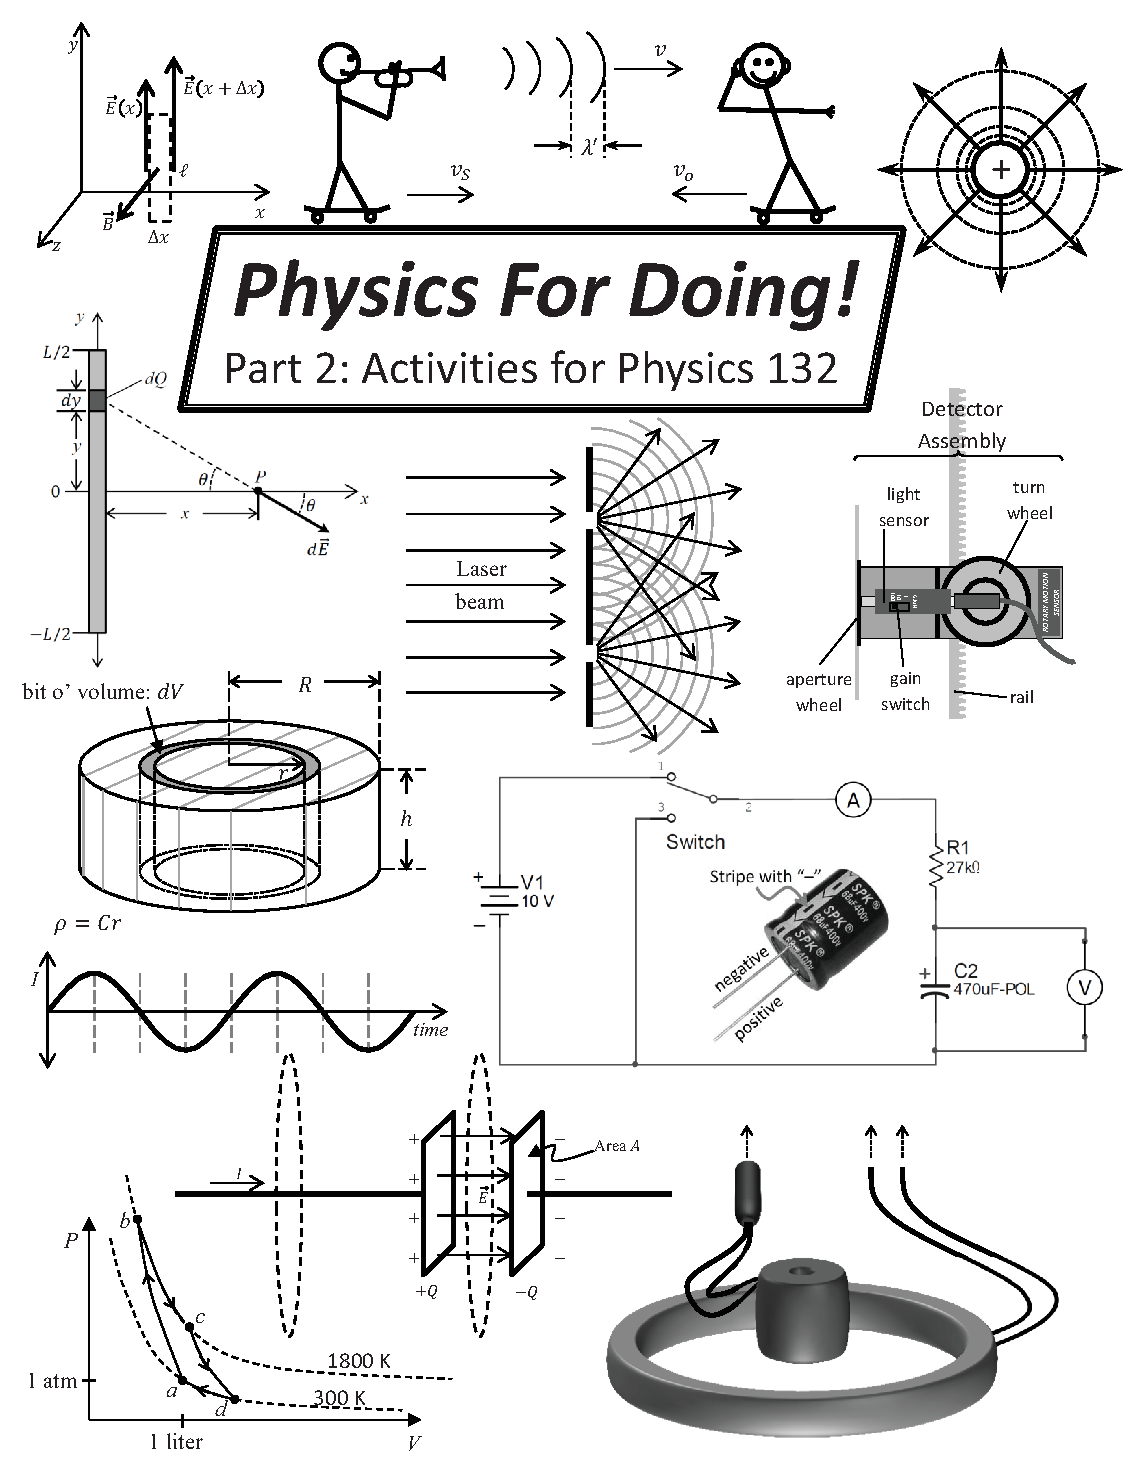
\includegraphics[width=7.3in,trim={0 0 .1cm 0},clip]{132_front_pages/132_front_cover.eps}
\index{color page}
\end{center}
\newpage

\restoregeometry
\restorepagecolor

\title{Physics For Doing!\\
Part 2: Activities for Physics 132}

\author{Emory F. Bunn, Mirela Fetea, Gerard P. Gilfoyle, Henry Nebel, \\
Philip D. Rubin, Jack Singal, Matthew L. Trawick, and Michael F. Vineyard\\[4pt]
Department of Physics, University of Richmond, VA \\[4pt]
%$^2$Department of Physics, George Mason University, Fairfax, VA \\[4pt]
%$^3$Department of Physics, Union College, Schenectady, NY \\[4pt]
%$^4$Germanna Community College, Fredericksburg, VA 22408
}

\maketitle

\vspace{0.5in}

%\begin{abstract}

\begin{center}
\large{\textbf{Welcome to Physics 132!}}
\end{center}

The exercises in this manual have been developed to support an investigative
physics course that emphasizes active learning. 
%The units are made up of activities designed to guide your investigations in the laboratory. 
Your written work will consist primarily of documenting
your class activities by filling in the entries in the spaces provided
in the units. The entries consist of observations, derivations, calculations,
and answers to questions. Although you may use the same data and graphs
as your partner(s) and discuss concepts with your classmates, all
entries should reflect your own understanding of the concepts and
the meaning of the data and graphs you are presenting. Thus, each
entry should be written in your own words. It is very important
to your success in this course that your entries reflect a sound understanding
of the phenomena you are observing and analyzing. 

Some of these units
have been taken from the Workshop Physics project at Dickinson College
and the Tools for Scientific Thinking project at Tufts University
and modified for use at the University of Richmond. Others have been
developed locally. 
We wish to acknowledge the support we have received for this project
from the University of Richmond and the Instrumentation and Laboratory
Improvement program of the National Science Foundation. Also, we would
like to thank our laboratory directors for their invaluable technical
assistance.
%\end{abstract}

%\begin{center}
%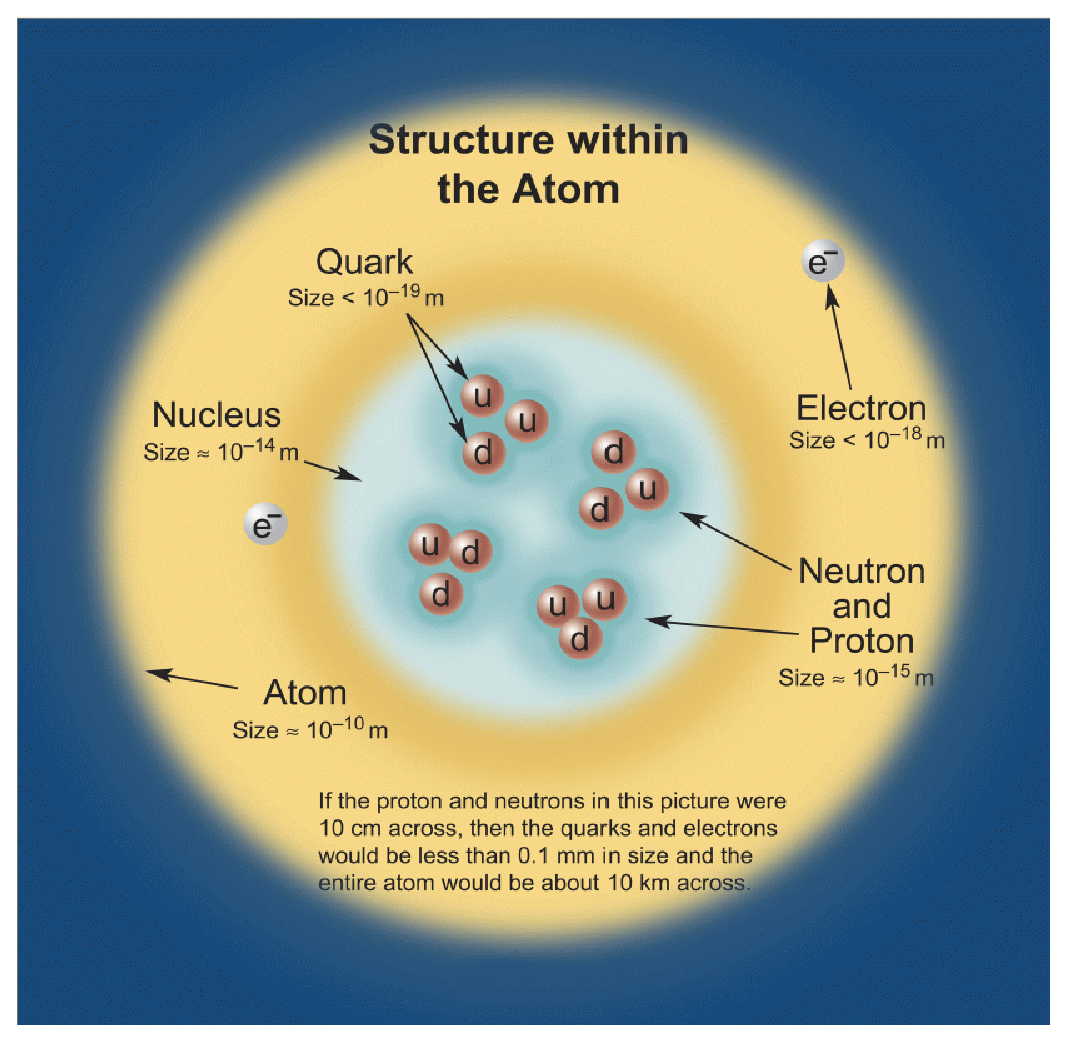
\includegraphics[width=3.2in]{132_front_pages/AtomicStructure.eps}
%\index{color page}
%\end{center}

\thispagestyle{plain}
%\thispagestyle{empty}

%\newpage

\
\setcounter{page}{2} %changed from 1 to 2 on 6/9/15 by MT.  The reason is that in the circuit labs, the odd pages need to be on the right (the fronts of each sheet of paper) and the even pages need to be on the left.  This is critical, because these labs have some pages that are meant to be cut out with scissors, so the backs have to be left blank.  This is done by using the \cleardoublepage command, which requires that the odd/even pages not be reversed from the usual.

\vfill

%Cover art: The atom consists of smaller electrons and a nucleus consisting of protons and neutrons. The protons and neutrons, in turn, are formed from objects called quarks and gluons. Courtesy, the American Institute of Physics.

\textit{Cover art: Various graphics and diagrams from the activities in this manual.  Yep, you'll be doing stuff.}

\pagebreak


\tableofcontents{}

%--------------------------------------------
\part{Mechanical Waves}
\
%This little backslash after the \part{} command is vital!  Without it, 
%the \include command doesn't play well with the \part command, and the first section (lab) of each part
%is wrongly listed as the last section of the previous part.
\section{Music to Our Ears: Standing Waves on Strings}

\makelabheader %(Space for student name, etc., defined in master.tex)

\begin{comment}
This lab was changed A LOT by Matt Trawick, 1/23/2016. Old version is saved as standing_waves_on_strings_old2015.tex.

1. Reduced the length of the background material.  Tightened up some of the exposition.  Also removed the parts that gave students the equation \lambda = 2L/n (twice!), on the grounds that students can figure it out themselves.  IMHO, the entire ``introduction'' part could still be removed and I wouldn't miss it.

2. Format changed to match the usual ``Activity 1'' etc.

3. Uncertainty is now done more consistently; students calculate uncertainty for v_A and v_B, not just v_A.

4. I removed the previous second section (`Part B') which had students change the masses to get different modes.  It's much more natural to change the frequency, and we have the equipment to do it easily.  Also, plotting T vs 1/n^2 seemed really old-timey.  And all for.... calculating the mass density, which you already knew from the scale anyway.

5.  The new section I put in instead (Activity 2) has students get different modes by changing frequency.  (This prepares them better for doing the same thing for the resonance tubes lab.)  I also have them derive, from pictures, the relationship 
f = (v/2L)n, which students always want to just memorize without thinking about it.
\end{comment}

\bigskip

\textbf{Apparatus}
\begin{itemize} [nosep] 
\item  String vibrator 
\item  Sine wave generator
\item  Inelastic braided string
\item  2 clamps
\item  Superpulley
\item  Mounting rod for the superpulley
\item  Mass and hanger set
\item  Precision balance
\item  Tape measure or meter stick
\end{itemize}

\bigskip
\textbf{Introduction}

How do we make musical sounds? To make a sound, we need something that vibrates. If we want to make musical notes you usually need the vibration to
have an almost constant frequency: that means stable pitch. We also want a frequency that can be easily controlled by the player. In electronic
instruments this is done with electric circuits or with clocks and memories. In non-electronic instruments, the stable, controlled vibration is
produced by a standing wave. Here we discuss the way strings work. This is also a good introduction for studying wind instruments, because vibrating
strings are easier to visualise than the vibration of the air in wind instruments, though the math is very similar.

Waves are oscillations in an elastic medium:
\begin{itemize}
\item  your own vocal cords (the medium) vibrating as air is forced over them by your lungs; 
\item  a stretched string (the medium) on a musical instrument vibrating as it is bowed, hammered or plucked; 
\item  pressure oscillations in a column of air (the medium) in a wind instrument, organ pipe or your own oral and nasal cavities.
\end{itemize}

In each case the medium has an equilibrium state, and when displaced or otherwise perturbed from that state, experiences a force which tends to
restore it to equilibrium. For small perturbations, the restoring force is proportional to the displacement and the medium becomes a simple harmonic
oscillator.


\textbf{Background}

\textbf{Standing waves} are produced by the interference of two traveling waves, both of which have the
same wavelength $\lambda$, speed $v$, and amplitude, but travel in opposite directions through the same medium. 
One way to get standing waves is with reflections, such as when a wave traveling along a stretched string reflects off the end.  The reflected wave travels backwards, interfering with the wave traveling forwards to produce a standing wave pattern on the string.  

One characteristic of every standing wave pattern is that there are points along the medium which appear to be standing still. These points,
sometimes described as points of no displacement, are referred to as \textbf{nodes}. Points in between the nodes that undergo the \textit{maximum} displacement between
large positive and large negative values are called \textbf{antinodes}. When a standing wave pattern is established in a medium, the locations of nodes and antinodes remain fixed and don't move; hence the name ``standing'' waves.  A particular arrangement of nodes and antinodes is called a \textbf{mode} of vibration.

The number of nodes and antinodes in a standing wave depends on the frequency of the wave as well as properties of the medium.  
If you drive a stretched string at an arbitrary frequency, you will probably not see any particular mode; many modes will be mixed together, and the overall amplitude will be small.
But, if the tension and the string's length are correctly adjusted to the frequency of the driving vibrator, one vibrational mode will occur at a much
greater amplitude than the other modes.

\begin{wrapfigure}[9]{r}{0.5\textwidth}
\vspace{-0.15in}
    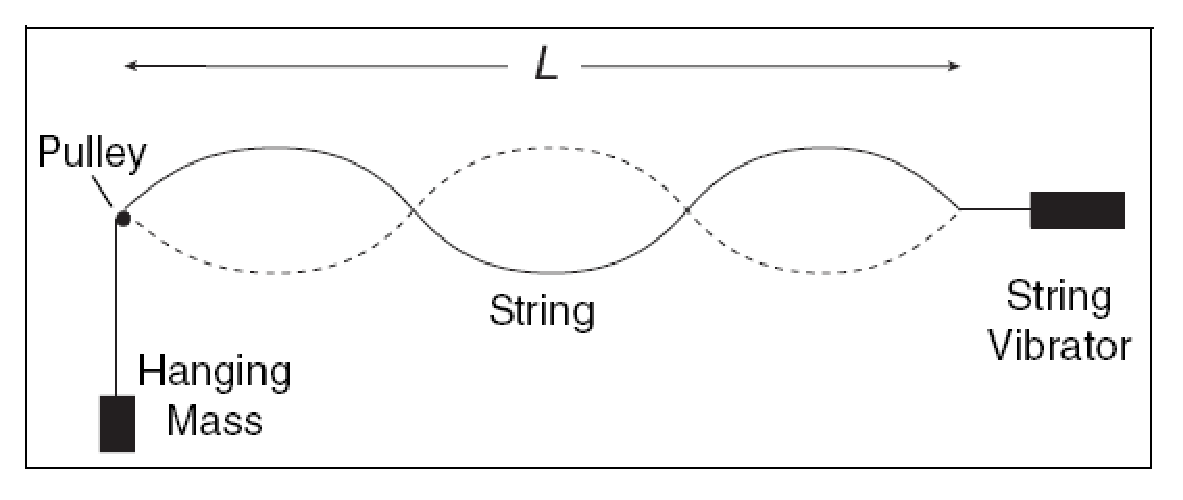
\includegraphics[width=0.5\textwidth]{standing_waves_strings/standing_waves_strings_fig2_tb.eps}
\end{wrapfigure}

\vspace{0.1in}
In this experiment, standing waves are set up in a stretched string by the vibrations of an electrically-driven string vibrator. The tension in the
string equals the weight of the masses suspended over the pulley. You can alter the tension by
changing the masses. 

%\vspace{0.3cm}
%\begin{center}
%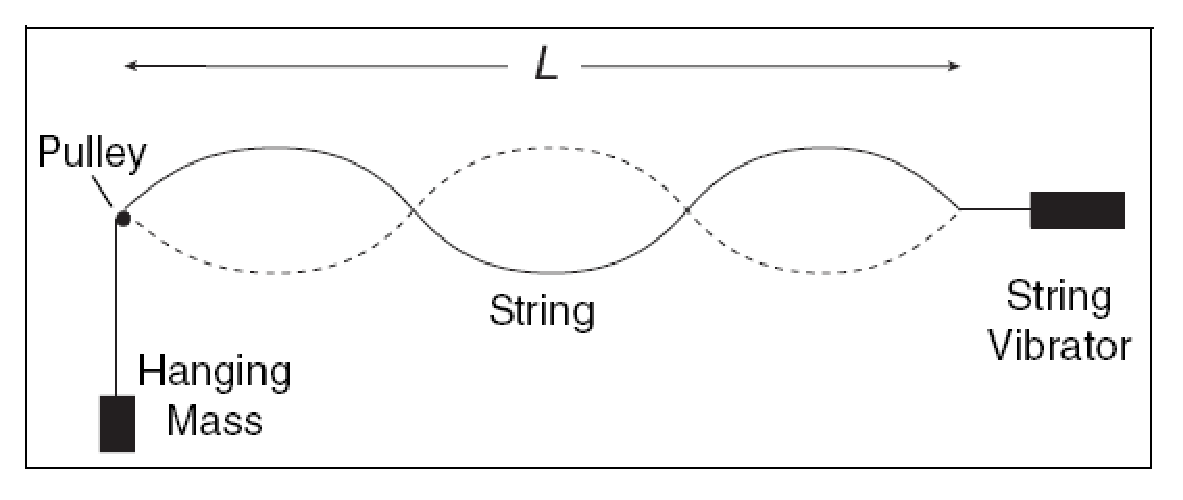
\includegraphics[width=250pt]{standing_waves_strings/standing_waves_strings_fig2_tb.eps}
%%\includegraphics[width=3in]{standing_waves_strings/standing_waves_strings_figure2.eps}
%\end{center}
%\vspace{0.3cm}

The speed of a wave on the string is given by:
\begin{equation*}
v=\sqrt{\frac {T}{\mu }}
\end{equation*}
where $T$ is the tension in the string and $\mu $ is the linear density (mass/length) of the string.  The speed of any wave is also related to its wavelength and frequency by
\begin{equation*}
v=\lambda f.
\end{equation*}


\textbf{Activity 1: Varying the tension and calculating the wave speed}

(a) Clamp the string vibrator and pulley about a meter apart. Attach the string to the vibrating blade, run it over the pulley, and hang about 200 g of mass from it. Cut off the excess string. Measure the distance $L$ from the knot where the string attaches to the string vibrator to the top of the pulley.
%This length $L$ is NOT the total length of the string that you measured in part (a). 

Record the value here, along with the uncertainty: $L$ =

\vspace{0.5cm}
\begin{center}
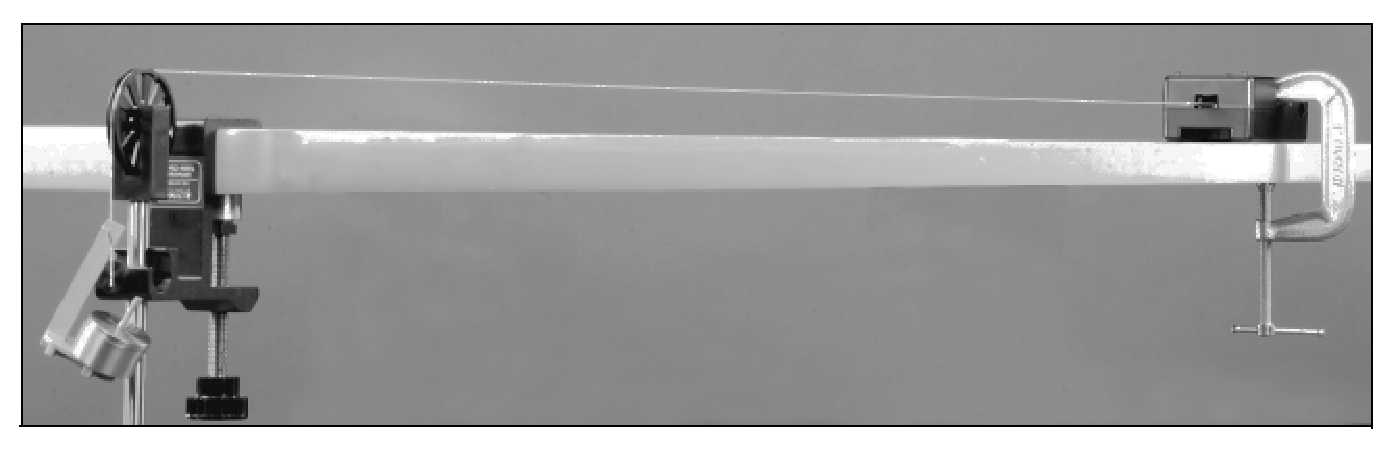
\includegraphics[width=320pt]{standing_waves_strings/standing_waves_strings_fig3_tb.eps}
\end{center}
%\vspace{0.1cm}

Connect the sine wave generator to the string vibrator. (There's a tiny switch in the back of the generator to turn it on.)  Adjust the frequency to 60.0 Hz, and adjust the amplitude to a moderately high value.

Change the tension by adding to or subtracting from the hanging mass so that the string vibrates in 2 segments. Adjust the tension to achieve a ``clean'' node at the center. Also check the end of the vibrating blade; the point where the string attaches should be a node. It is more important to have a good node at the blade than it is to have the largest amplitude possible. However, it is desirable to have the largest amplitude possible while keeping a good node.

(b) Record the best value of the hanging mass, $m$. How much uncertainty is there in that best value? (That is, by how much can you change the hanging mass before you see an effect?) Record the uncertainty too.
\answerspace{2cm}

\pagebreak[2]

(c) Use your mass to calculate the tension $T$ (including the uncertainty) in the string.
\answerspace{2cm}

(d) Measure the exact length of another piece of string several meters long (not the one connected to the string vibrator). Measure the mass of the
string and calculate the linear density $\mu$ (mass/length).  
%(If your balance is not precise enough to measure that length of string, use a longer piece of string.)  
Be sure to estimate the uncertainties in both the mass and the length, bearing in mind that the string can stretch. What is the resulting uncertainty in $\mu$?  (For help with uncertainties, refer to Appendix \ref{uncertainty}.)
\answerspace{4.5cm}

\pagebreak[3]

(e) Calculate the speed $v_A$ of the wave from your observed values of tension
$T$ and linear density $\mu$. Record your calculated value with the uncertainty and the correct number of significant
figures.
\answerspace{4cm}

(f) Calculate the speed $v_B$ from the wavelength ($\lambda $) and frequency ($f$).  What are your uncertainties in $\lambda$ and $f$?  What is your uncertainty in $v_B?$
\answerspace{4cm}

(g) Compare the two values of speed, $v_A$ and $v_B$.  Are the two consistent, to within the uncertainties you calculated?  That is, do their ranges overlap?  (If not, you have some explaining to do....) 
\answerspace{3cm}

\pagebreak[2]
\textbf{Activity 2: Vibrational modes at different frequencies}

\textit{For this part, keep the same string length as in Activity 1, and keep about 200 grams on the end of the string.}

(a) In Activity 1, the standing wave on the string had one node in the middle, dividing the string into $n=2$ vibrating segments.  This means that the standing wave had $n=2$ antinodes.  Change the frequency to find both higher and lower values of $f$ that produce standing waves with different numbers of antinodes.  Record your results in the table below.
\begin{center} 
\begin{tabular}{|c|c|} 
\hline $\mathbf{n}$ & \boldmath$f$ \textbf{(Hz)} \\ 
\hline 1 &  \\ 
\hline 2 &  \\ 
\hline 3 &  \\ 
\hline 4 &  \\ 
\hline 5 &  \\ 
\hline 6 &  \\ 
\hline 7 &  \\ 
\hline 
\end{tabular} 
\end{center}

(\textit{You may need to adjust the amplitude knob to keep the standing wave a reasonable size.  Also, don't worry if the last few modes are too hard to see.  Finally, there's a weird resonance within the string vibrator itself that makes it wonky around 150 Hz; just ignore that and skip past it if necessary.})

\pagebreak[3]

(b) On the lines below, draw pictures of the first three standing wave modes you found.  For each drawing, write the relationship between the half wavelength $\frac{1}{2}\lambda$ and the string length $L$.

\begin{center}
$n=1$: 
\raisebox{-0.15in}{\rule{3pt}{0.4in}}\raisebox{.05in}{\rule{2.5in}{0.1pt}}\raisebox{-0.15in}{\rule{3pt}{0.4in}}
\hspace{0.3in}$\frac{1}{2}\lambda=$

$n=2$:
\raisebox{-0.15in}{\rule{3pt}{0.4in}}\raisebox{.05in}{\rule{2.5in}{0.1pt}}\raisebox{-0.15in}{\rule{3pt}{0.4in}}
\hspace{0.3in}$\frac{1}{2}\lambda=$

$n=3$:
\raisebox{-0.15in}{\rule{3pt}{0.4in}}\raisebox{.05in}{\rule{2.5in}{0.1pt}}\raisebox{-0.15in}{\rule{3pt}{0.4in}}
\hspace{0.3in}$\frac{1}{2}\lambda=$
\end{center}
%axes

(c) From your three pictures above, write a general equation relating $\lambda$ and $L$ for each possible value of $n$.
\answerspace{2cm}

(d) Using the relationship between $\lambda$, $f$, and $v$, rewrite your equation in (c) to express the frequency $f$ for each value of $n$, in terms of $n$, $v$, and $L$.
\answerspace{2cm}

(e) If you were to make a graph of $f$ \textit{vs.} $n$, what would be the slope of that graph, in terms of $v$ and $L$?
\answerspace{2cm}

\pagebreak[3]
(f) Plot a graph of your data for $f$ \textit{vs.} $n$ from part (a) using Excel.\footnote{In general, ``plot $A$ \textit{vs.} $B$'' means ``plot $A$ as a function of $B$,'' which implies that thing $B$ should go on the horizontal axis.} Use the LINEST function to determine the slope of the graph and its uncertainty. (See Appendix \ref{excel} for help using Excel's LINEST function.)  Do you want LINEST to estimate the $y$-intercept, or force it to zero?  Record the slope and its uncertainty here.
\answerspace{3cm}



(g) Does the uncertainty in the slope given by LINEST capture \textit{all} sources of uncertainty in your measurement?
\answerspace{2cm}

(h) Using your values from (f), calculate the velocity of the wave and its uncertainty. 
\answerspace{4cm}

(i) Is the velocity you just calculated consistent with the values $v_A$ and $v_B$ you calculated in Activity 1?  
\answerspace{3cm}


%\textbf{Further Investigation}
%
%If a strobe is available, observe the standing wave on a string with the 
%strobe light. Draw a diagram explaining the motion of the string.





\section{Resonance in Tubes}

\makelabheader %(Space for student name, etc., defined in master.tex)

\bigskip

\textbf{Objectives}
\begin{itemize}[nosep]
\item Determine the resonant frequency for a tube open at one end.

\item Determine tube lengths at resonance for a tube of variable length.

\item Determine the velocity of sound in air in the laboratory (two ways).

\end{itemize}

\bigskip
\textbf{Apparatus} 
\begin{itemize}[nosep]

\item Economy Resonance Tube 
\item Open speaker
\item Sine wave generator
\item 2 banana plug leads
\item Sound sensor
\item Meter stick
\item Pasco 550 Interface
\item Thermometer

\end{itemize}
\bigskip
\textbf{Introduction} 

The Economy Resonance Tube is designed for the study of resonance in columns of air.  The tube set includes a movable inner tube with a closed end and an outer tube which is open at both ends.  The inner tube also includes a measuring tape to easily find the length of the air column in the outer tube.  To adjust the length of the outer tube, simply slide the inner tube until the desired length appears on the measuring tape.  Open tube experiments can also be performed with the outer tube by removing the inner tube.

In order that the tube resonate, the frequency of the vibrating air must coincide with the natural frequency of the tube (which may be its fundamental or one of its overtones). For the Economy Resonance Tube, which is closed at one end, this requirement is met if the tube length is an odd number of quarter wavelengths of the sound waves produced by the source ($L = \lambda/4, 3 \lambda/4, 5 \lambda/4$, etc., where $L$ is the length of the tube and $\lambda$ is the wave length of the sound). Note that if the length of the tube is gradually increased while the source is vibrating, the distance between successive resonance positions is $\lambda/2$. 

\textbf{Note:} Due to edge effects at the open end of a tube, the effective length of the tube depends on the radius of the opening. Thus, $L_{eff} = L + 0.6r$, where $L_{eff}$ is the \textit{effective} length, $L$ is the length measured, and $r$ is the tube radius.

\medskip
Room Temperature ($^\circ$C) \hrulefill \ \  Tube radius (m) \hrulefill

\bigskip

\textbf{Activity 1: Fixed Tube Length} 
\begin{enumerate}[labparts]

\item Connect the open speaker to the sine wave generator using standard banana plug leads.

\item Adjust the length of the OUTER (blue) tube to 80 cm (check with meter stick).

\item Place the tube in front of the speaker in such a way that the tube is open at one end (the speaker can be set at an angle relative to the tube length).

\item Set the sound sensor inside the tube at the open end and connect it to the Data Studio interface.

\item To activate the sound sensor, perform the following sequence:  Start up \textit{DataStudio} by going to \textit{Start} $\rightarrow$ \textit{Programs} $\rightarrow$ \textit{Physics Applications} $\rightarrow$ \textit{DataStudio}.
Click on \textit{Create Experiment}, then \textit{Setup}, then \textit{Add Sensor or Instrument}. Scroll down to \textit{Sound level sensor} and select, then click \textit{OK}. Double click \textit{Graph} at left. Click \textit{Start} to begin taking data.

\item The resonant frequencies for a tube open at one end are given by $f=nv/4L$ where $n$ is an odd integer, $v$ is the velocity of sound and $L$ is the effective tube length. Start at a frequency of 50 Hz and increase to 800 Hz, noting any resonances you find.   These will be indicated by peaks on the sound level graph. You need to carefully determine the frequency associated with each peak.  Record the results below. (Note: the speakers themselves have small mechanical resonances at about 140 Hz and 200 Hz; these aren't the ones you're looking for.)
\vspace{10mm}

\item From your data, plot a graph of $f$ \textit{vs.} $n$ using Excel.\footnote{In general, ``plot $A$ \textit{vs.} $B$'' means ``plot $A$ as a function of $B$,'' which implies that thing $B$ should go on the horizontal axis.} Fit with a linear trendline. Print the graph (with title and axis labels) and include with this unit. Use the LINEST function in Excel to determine the slope of the graph and its uncertainty. From these values, calculate the velocity of sound in air, and its uncertainty, and record them here. Don't forget to use $L_{eff}$ - see Introduction.
\vspace{12mm}

\end{enumerate}

%\noindent {\Large{\bf DATA}} \\

%\noindent Room Temperature ($^\circ$C) \hrulefill \ \  Tube radius (m) \hrulefill

%\begin{center} \begin{tabular}{||c|c|c|c|c|c|c|c|c|c|c|c|c|c|c||} \hline \hline Tuning Fork & \multicolumn{4}{|c|}{First Position of} & \multicolumn{4}{|c|}{Second Position} & \multicolumn{4}{|c|}{Third Position of} & Wave- & Velocity of \\ Frequency, & \multicolumn{4}{|c|}{Resonance, m} & \multicolumn{4}{|c|}{of Resonance, m} & \multicolumn{4}{|c|}{Resonance, m} & length, & Sound in \\ \cline{2-13} Hz & 1 & 2 & 3 & Ave. & 1 & 2 & 3 & Ave. & 1 & 2 & 3 & Ave. & m & air, m/s \\ \hline \hline &&&&&&&&&&&&&& \\ \hline &&&&&&&&&&&&&& \\ \hline \hline \end{tabular} \end{center}


\textbf{Activity 2: Fixed Frequency} 

Adjust the outer tube length to 20~cm, and set the sine wave generator frequency to 600 Hz (with low amplitude).
Place the speaker inside the open end of the tube so that the tube is effectively closed at both ends. (Do not include the sound sensor for this activity. You will just be listening for loudness.)

\begin{enumerate}[labparts]
\item Slowly move the inner tube to increase the effective length of the tube. Listen for maximum loudness and record the length of the tube when resonance is achieved:
\vspace{10mm}

\item Increase the length of the tube until two more resonance lengths are found for the constant frequency and record them here:
\vspace{10mm}

%\item Average your two values to determine your experimental velocity of sound in m/s: \ \ \  \rule{2cm}{1pt}

\item The resonant frequencies for a tube closed at both ends are given by 
$f=nv/2L$ where $n$ = 1, 2, 3, etc. Solve this equation for $L$ and plot $L$ 
vs. $n$ (using Excel) where $n$ = 1, 2 and 3 for the three resonance lengths $L$
you found in (d) and (e) above. Fit with a linear trendline. Use the LINEST function in Excel to determine the slope of the graph and its uncertainty. Use these values to determine the velocity of sound in air and its uncertainty and record them here:
\vspace{20mm}

\item The velocity of sound in air at $0^\circ$C is 331.4 m/s.  The temperature dependence of sound velocity in air is given by $v(T) = 331.4 + 0.6T$, where $T$ is in $^\circ$C and $v$ is in m/s. Calculate an ``accepted'' value of the velocity of sound in air from this formula.
\vspace{20mm}

\item Does the ``accepted'' value fall within the range of uncertainty of your experimental value?
\answerspace{5mm}
\end{enumerate}

\include*{doppler_shift/doppler_shift}
%Also Note that the \include*{} command is used before each new \part{} to avoid an extra blank page.
%This is an awkard fix, and somebody else welcome to find a better solution.

%--------------------------------------------
\part{Electrostatics}
\
	\include{electrostatics}
	
\section{The Interactions of Electric Charges\footnote{%
Adapted from A. Arons, \underbar{A Guide to Introductory Physics Teaching},
Wiley \& Sons, 1990; and R. Chabay and B. Sherwood, \underbar{Electric
\& Magnetic Interactions}, Wiley \& Sons, 1995.
}}

Name \rule{2.0in}{0.1pt}\hfill{}Section \rule{1.0in}{0.1pt}\hfill{}Date
\rule{1.0in}{0.1pt}

\textbf{Objectives}

\begin{itemize}
\item Note the number of different kinds of charge
\item Characterize the interactions between like and unlike charges
\item Discover the nature of electrical force
\end{itemize}
\textbf{Introduction}

You probably already know this, but electric force between charge
objects is proportional to the amount of charge on each of the objects,
acts along a line between the objects, and decreases rapidly as the
distance between the two objects increases. In the following activities,
you will find out if invisible tape exhibits these properties, and
thus whether such tape becomes electrically charged and therefore
useful in the study of electrical interactions. Use strips of tape
around 20 cm long. Shorter pieces are too inflexible; longer ones
too difficult to handle. Fold one end of each strip to make a non-stick
handle and stick a paper clip on this handle.

Note: The real world is messy. Straight-forward experimental manipulations
and accurate measurements are not always easy to come by. Try to keep
your frustration level down. Rough observations are good enough for
this lab.

\textbf{Apparatus}

\begin{itemize}
\item Invisible ({}``Scotch'') tape
\item Paper clips (2)
\end{itemize}
\textbf{Investigation 1: Your Hand and a U Tape}

\textbf{Preparing a U Tape:}

\begin{enumerate}
\item Stick a strip of tape, sticky-side down, onto the table top and smooth
it down with your thumb or fingers. This base tape provides a standard
work surface and thus ensures consistent results.
\item Stick a second strip of tape, sticky-side down, on top of the base
tape and smooth it down well with thumb or fingertips. Write the letter
U (for Upper) on the handle of this strip.
\item Holding the handle and with a very quick motion, pull the U tape up
and off the base tape, which should remain stuck to the table.
\end{enumerate}
\textbf{Activity:}

\begin{enumerate}
\item Hang the U tape vertically from the edge of the table, handle down.
\item Briefly describe what happens when you slowly bring your hand near
the hanging tape.\vspace{15mm}

\item Is the behavior different when you approach the other side of the
tape?\vspace{15mm}

\end{enumerate}
\textbf{Note:} Tape should react to the presence of your hand. If
not, repeat the U tape preparation.

\textbf{Prediction:} How would you expect two U tapes to interact:
repel each other, attract each other, or not affect each other? Briefly
explain your reasoning.
\vspace{1in}

\textbf{Investigation 2: Two U Tapes}

\textbf{Activity 1:}

\begin{enumerate}
\item Prepare a second U tape, remembering to mark U on its handle.
\item Doing your best to keep your hand out of the way (recall that your
hand attracts the tape--perhaps hold the second strip horizontally
in two hands), bring the second U tape near the hanging first one.
Describe what happens.\vspace{15mm}

\item Hand the second U tape beside the first.
\end{enumerate}
\textbf{Activity 2:}

\begin{enumerate}
\item Suspend a U tape from a piece of thread or hair.
\item Approach the suspended tape from various directions with the other
U tape. Do the tapes repel along or at an angle to the line between
the objects?
\end{enumerate}
\vspace{0.3cm}
{\centering 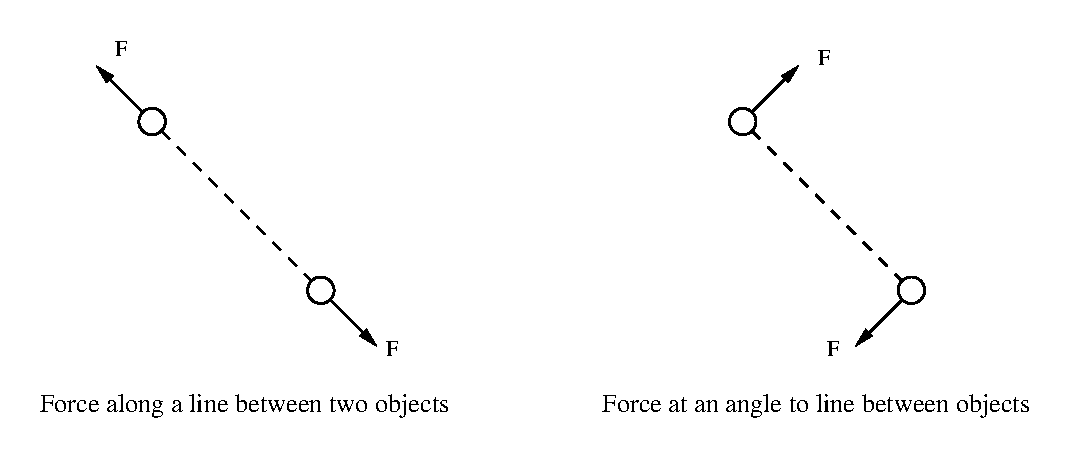
\includegraphics{int_elec_charges_fig_1.eps} \par}
\vspace{0.3cm}

\vspace{15mm}
\textbf{Note:} You may have noticed that if you handle a U tape too
much, it loses its interaction strength. Remember to reactivate the
strips regularly.

\textbf{Activity 3:}

\begin{enumerate}
\item Note that when you move one U tape slowly toward a hanging U tape,
there is a distance at which repulsion is first detectable.
\item Note what happens as you repeatedly halve the distance between the
strips.\vspace{15mm}

\item Graph--very roughly--the deflection of the hanging tape as a function
of the distance between tapes. Note that this deflection from an original
vertical position is a measure of the strength of the interaction.
\end{enumerate}
\vspace{0.3cm}
{\centering \includegraphics{int_elec_charges_fig_2.eps} \par}
\vspace{0.3cm}

\textbf{Activity 4:}

\begin{enumerate}
\item Hold the bottom of a hanging, active U tape and slowly rub your thumb
or fingers back and forth along its slick side.
\item Describe the changes in how this U tape interacts with your hand.
Also, with another U tape.\vspace{15mm}

\item Reactivate two U tapes. Hang one from the table and note how strongly
the other one repels it.\vspace{15mm}

\item Run a finger along the length of the hanging tape's slick side, but
touch only a portion of its width (not the full side). Be sure to
leave a continuous vertical section untouched. 
\item Do the two tapes now exhibit a weaker or stronger repulsion, or no
repulsion at all?\vspace{15mm}

\item Try to explain what has been going on in this activity.\vspace{15mm}

\end{enumerate}
\textbf{Questions:}

\begin{enumerate}
\item Are U tapes electrically charged?\vspace{10mm}

\item Do U tapes have like or unlike electric charge?\vspace{10mm}

\end{enumerate}
\textbf{Investigation 3: A U and an L Tape}

\textbf{Challenge:} How would you prepare a tape that might have an
electric charge unlike the charge on a U tape?

\textbf{Preparing an L Tape:}

\begin{enumerate}
\item Stick a strip of tape, sticky-side down, on top of the base tape and
smooth it down well with thumb or fingertips. Write the letter L (for
Lower) on the handle of this strip.
\item Stick a second strip of tape, sticky-side down, on top of the L tape
and smooth it down well with thumb or fingertips. Write the letter
U (for Upper) on the handle of this strip.
\item Lifting the handle of the L tape, slowly pull it along with the U
tape up and off the base tape, which should remain stuck to the table.
\item Hang the double layer of tape vertically from the edge of the table,
handles down. Check that there is no interaction between it and your
hand. If there is, do what you need to so the interaction no longer
occurs.
\item While holding down the handle of the L tape, quickly life off the
U tape, then hang it vertically from the edge of the table, not too
close to the L tape.
\end{enumerate}
\textbf{Prediction:} Will the L tape attract, repel, or not interact
with the U tape if the two are brought within proximity of one another?
\vspace{1in}

\textbf{Activity 1:}

\begin{enumerate}
\item With your hand, check that both the U tape and the L tape are active.
How can you tell?\vspace{15mm}

\item What interaction do you observe between an L tape and a U tape?\vspace{15mm}

\end{enumerate}
\textbf{Prediction:} Will an L tape attract, repel, or not interact
with another L tape if the two are brought within proximity of one
another?
\vspace{15mm}

\textbf{Activity 2:}

\begin{enumerate}
\item Make another pair of L and U tapes.
\item Be sure that all four tapes are active.
\item What interaction do you observe between two L tapes?\vspace{15mm}

\item Summarize the interactions you have observed between U and L tapes:
\end{enumerate}
\begin{quote}
L-U:

U-U:

L-L:
\end{quote}
~~~~5.~State a rule for the pattern of interactions between like
and unlike charges:
\vspace{20mm}

\textbf{Activity 3:}

\begin{enumerate}
\item Note that when you move an active L tape slowly toward a hanging U
tape, there is a distance at which attraction is first detectable.
\item Note what happens as you repeatedly halve the distance between the
strips.\vspace{15mm}

\item Graph--very roughly--the deflection of the hanging tape as a function
of the distance between tapes. Note that this deflection from an original
vertical position is a measure of the strength of the interaction.
\end{enumerate}
\vspace{0.3cm}
{\centering \includegraphics{int_elec_charges_fig_3.eps} \par}
\vspace{0.3cm}

\textbf{Questions:}

\begin{enumerate}
\item Why is this task more difficult now than it was with two U tapes?\vspace{15mm}

\item Do the forces between U and L tapes lie along or at an angle to the
line between the tapes?
\end{enumerate}
\begin{quotation}
Force by U tape on L tape:
\vspace{10mm}

Force by L tape on U tape:\vspace{10mm}

\end{quotation}
\textbf{Summary:} In the table below, state very briefly what you
observed.

\vspace{0.3cm}
{\centering \begin{tabular}{|l|l|}
\hline 
~~~~~~~~~~~~~~~~~~~~~~~~~~~~~~~~\textbf{Property}&
\textbf{Experimental Observation of U and L Tapes}\\
\hline
\hline 
There are two kinds of charges;&
U-U:\\
like charges repel;&
L-L:\\
unlike charges attract.&
U-L:\\
\hline 
Electric force is proportional to amount of charge.&
U tape and partially neutralized U tape:\\
&
\\
\hline 
Electric force acts along a line between charges.&
U-U:\\
&
U-L:\\
\hline 
The strength of interaction decreases&
U-U:\\
rapidly as distance between the charges increases.&
U-L:\\
\hline
\end{tabular}\par}
\vspace{0.3cm}

\textbf{Activity 4:}

\begin{enumerate}
\item Quickly lift off the base tape.
\item Is it U-like or L-like? How can you tell?\vspace{15mm}

\end{enumerate}
\textbf{Questions:}

\begin{enumerate}
\item How does all of this happen: How do the tapes become charged? Why
are both U and L tapes attracted to your hand? Why does rubbing the
slick side of a tape with your finger appear to neutralize the tape?\vspace{20mm}

\item What do you think charges are?\vspace{15mm}
\end{enumerate}

 %not used in 2015
\section{Charge, Charge Density, and Fun with Integrals}

\begin{comment}
This lab is more of a worksheet than it is a lab.  But I've used versions of if in my 132 classes for a while, so I thought it was time to include it here in the lab manual for others as well.  

I find this kind of exercise is important to do, because students typically suck at setting up this kind of integral, where instead of just dx, they have dstuff, where the ``stuff'' actually means something.  They'll need to do this later when they set up integrals over dQ to find field or potential, and it's good for them to get some practice earlier when they only need to worry about Q.   

--Matt Trawick, 7/2015

\end{comment}

\makelabheader %(Space for student name, etc., defined in master.tex)

\vspace{0.1in}
\textbf{Objective:} To practice setting up integrals over $dQ$, and get more comfortable with charge densities.

\vspace{0.1in}
The total amount of electric charge on a whole object is usually denoted by the letter $Q$. But sometimes we are interested in the distribution of the charge over an object, in which case we need the ``charge density.''  For a thin rod or wire, we usually use $\lambda$ for the linear charge density, or charge per unit length, where $Q = \lambda \ell$. For thicker objects, we use $\rho$ (pronounced ``rho'') for the charge per unit volume, where $Q = \rho V$.  (Those equations are true as long as the charge is spread out evenly, so that the charge density is ``uniform.'')

1. In the pictures below, the thin rod and the rectangular block each have two \textit{different} charge densities.  Write the total charge $Q$ for each of them, in terms of the variables given in the pictures.
\begin{center}
\includegraphics[width=0.75\textwidth]{charge_density/fig1.eps}
\end{center}

2. In general, if there are lots of bits o' charge $\Delta Q$, then the total charge is given by their sum, $Q = \sum_i \Delta Q_i$. For the thin rod, you just used $\Delta Q_i = \lambda_i \Delta x$.  For the rectangular bar in the figure below, express the bit o' charge $\Delta Q_i$ in terms of the quantities given in the picture: $h$, $w$, $\Delta x$ and $\rho_i$

\vspace{-0.2 in}
\begin{center}
\includegraphics[width=0.75\textwidth]{charge_density/fig2.eps}
\vspace{-0.2in}
\end{center}
What if, instead of a finite number of uniform charge densities, the charge distribution on your object varies continuously, forming a smooth gradient. Instead of a discrete set of $\lambda_i$, your charge density would be some continuous function of position like $\lambda(x)$.  (That is, lambda as a function of $x$, not lambda times $x$.) No problem! Just imagine your finite $\Delta Q$ shrinking to an infinitesimal $dQ$.  For the thin rod, instead of $Q= \sum_i \Delta Q_i = \sum \lambda_i \Delta x$, you would use $Q = \int dQ = \int \lambda \left(x\right) dx$. 

%\begin{center}
%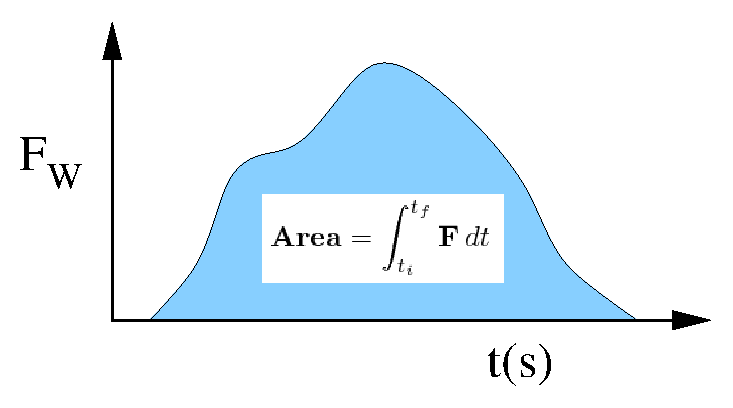
\includegraphics[width=0.35\textwidth]{charge_density/fig3.eps}
%\end{center}
\begin{wrapfigure}[4]{r}{0.4\textwidth}
\vspace{-0.4 in}
    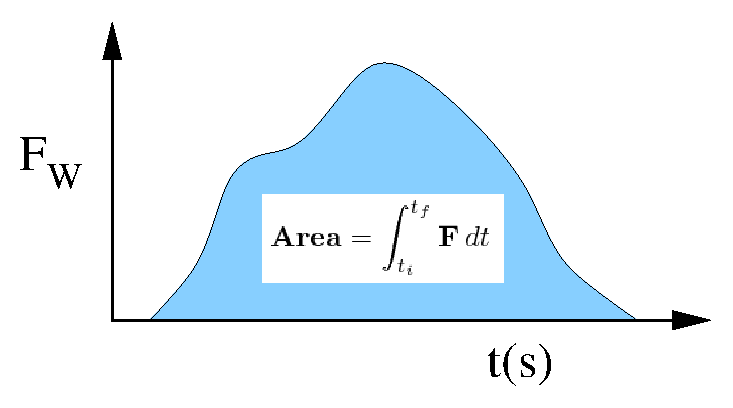
\includegraphics[width=0.4\textwidth]{charge_density/fig3.eps}
\end{wrapfigure}
\vspace{0.2 in}
3. In the picture to the right, suppose $\lambda = Cx$, where $C$ is some constant. Write the integral to find the total charge $Q$ of the rod, starting with $Q = \int dQ$, including the limits of integration.  Evaluate the integral to get $Q$.

\newpage

In the picture below, suppose $\rho = Cx^2$, where $C$ is some constant. To find the total charge $Q$, you will again use $Q = \int dQ$, but this time you'll write $dQ = \rho \,dV$.  
\vspace{-0.2 in}
\begin{center}
\includegraphics[width=0.40\textwidth]{charge_density/fig4.eps}
\end{center}

4.  What is $dV$, in terms of quantities given in the picture?
\vspace{0.3in}

5.  Write the integral, with limits, to find the total charge $Q$ of the block.  Evaluate the integral to get $Q$.
\vspace{1.0in}

Finally, we'll consider a solid cylinder of charge with height $h$ and radius $R$, where the charge density varies as $\rho = Cr$.  Again, we'll find the total charge by setting up an integral. 

For the rectangular block, we cut it into slices along the $x$ axis, so that each slice only had one value of $\rho$.  To cut the cylinder so that each slice has only one value of $\rho$, we'll have to cut it into concentric rings of radius $r$ like the picture below, then imagine unrolling each ring into a thin rectangular sheet.

\begin{center}
\includegraphics[width=0.85\textwidth]{charge_density/cylinders.eps}
\end{center}

6. What is the volume $dV$ of the thin rectangular sheet, expressed in terms of the quantities given in the picture above?
\vspace{0.3in}

7. Find the charge $Q$ of the cylinder by evaluating an integral over $dr$, starting with $Q = \int dQ$.  What are the limits of integration? 




	
\section{The Electrical and Gravitational Forces\footnote{
1990-93 Dept. of Physics and Astronomy, Dickinson College. Supported by FIPSE
(U.S. Dept. of Ed.) and NSF. Portions of this material have been modified locally
and may not have been classroom tested at Dickinson College.
} }

Name \rule{2.0in}{0.1pt}\hfill{}Section \rule{1.0in}{0.1pt}\hfill{}Date \rule{1.0in}{0.1pt}

\begin{quote}
I began to think of gravity extending to the orb of the moon, and . . . I deduced
that the forces which keep the planets in their orbs must be reciprocally as
the squares of their distances from the centers about which they revolve: and
thereby compared the force requisite to keep the moon in her orb with the force
of gravity at the surface of the earth, and found them to answer pretty nearly.
All this was in the two plague years of 1665 and 1666, for in those days I was
in the prime of my age for invention, and minded mathematics and philosophy
more than at any time since. - Isaac Newton 
\end{quote}
\textbf{Objective }

To understand the similarities of the gravitational and electrical forces. 

\textbf{Overview }

The enterprise of physics is concerned ultimately with mathematically describing
the fundamental forces of nature. Nature offers us several fundamental forces,
which include a strong force that holds the nuclei of atoms together, a weak
force that helps us describe certain kinds of radioactive decay in the nucleus,
the force of gravity, and the electromagnetic force. 

\textit{Two kinds of force dominate our everyday reality-the gravitational force
acting between masses and the Coulomb force acting between electrical charges.}
The gravitational force allows us to describe mathematically how objects near
the surface of the earth are attracted toward the earth and how the moon revolves
around the earth and planets revolve around the sun. The genius of Newton was
to realize that objects as diverse as falling apples and revolving planets are
both moving under the action of the same gravitational force. 

\vspace{0.3cm}
{\par\centering 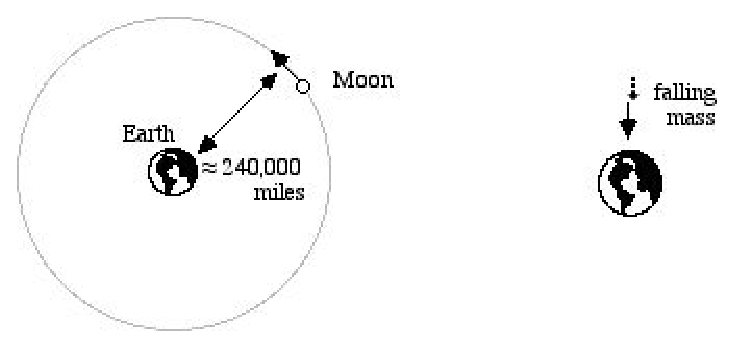
\includegraphics{elec_grav/elec_grav_fig1.eps} \par}
\vspace{0.3cm}

Similarly, the Coulomb force allows us to describe how one charge \char`\"{}falls\char`\"{}
toward another or how an electron orbits a proton in a hydrogen atom. 

\vspace{0.3cm}
{\par\centering 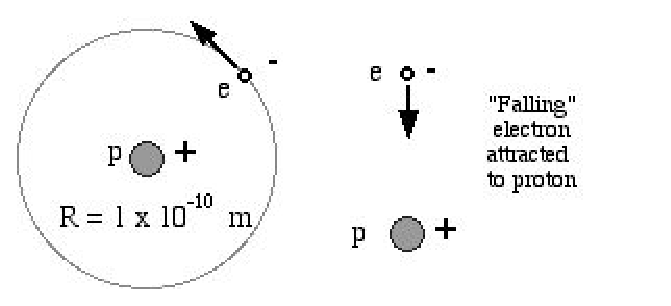
\includegraphics{elec_grav/elec_grav_fig2.eps} \par}
\vspace{0.3cm}

The fact that both the Coulomb and the gravitational forces lead to objects
falling and to objects orbiting around each other suggests that these forces
might have the same mathematical form. 

In this unit we will explore the mathematical symmetry between electrical and
gravitational forces for two reasons. First, it is beautiful to behold the unity
that nature offers us as we use the same type of mathematics to predict the
motion of planets and galaxies, the falling of objects, the flow of electrons
in circuits, and the nature of the hydrogen atom and of other chemical elements.
Second, what you have already learned about the influence of the gravitational
force on a mass can be applied to aid your understanding of the forces on charged
particles. 

\textbf{Activity 1: Comparison of Electrical and Gravitational Forces }

Let's start our discussion of this comparison with the familiar expression of
the Coulomb force exerted on charge 1 by charge 2. 

\vspace{0.3cm}
{\par\centering 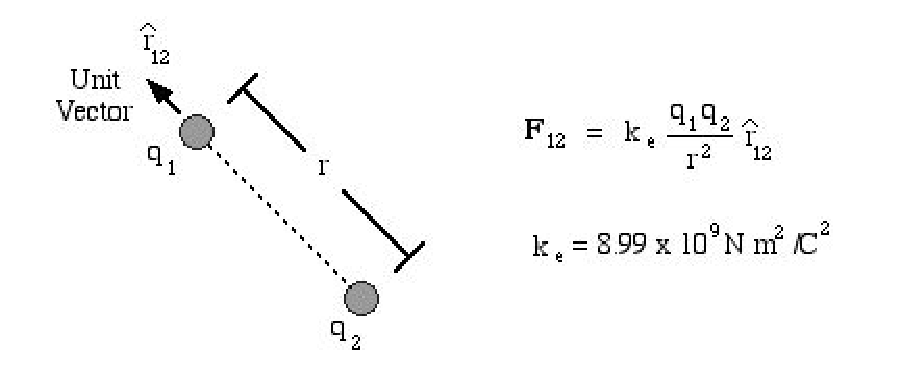
\includegraphics{elec_grav/elec_grav_fig3.eps} \par}
\vspace{0.3cm}

Charles Coulomb did his experimental investigations of this force in the 18th
century by exploring the forces between two small charged spheres. Much later,
in the 20th century, Coulomb's law enabled scientists to design cyclotrons and
other types of accelerators for moving charged particles in circular orbits
at high speeds. 

Newton's discovery of the universal law of gravitation came the other way around.
He thought about orbits first. This was back in the 17th century, long before
Coulomb began his studies. A statement of Newton's universal law of gravitation
describing the force experienced by mass 1 due to the presence of mass 2 is
shown below in modern mathematical notation: 

\vspace{0.3cm}
{\par\centering 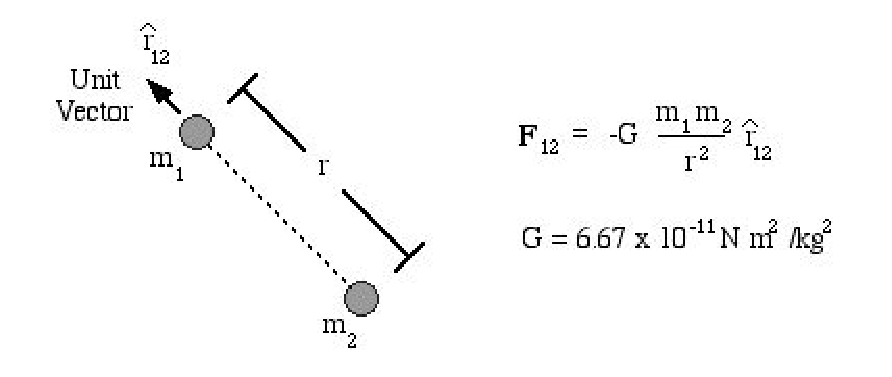
\includegraphics{elec_grav/elec_grav_fig4.eps} \par}
\vspace{0.3cm}

About the time that Coulomb did his experiments with electrical charges in the
18th century, one of his contemporaries, Henry Cavendish, did a direct experiment
to determine the nature of the gravitational force between two spherical masses
in a laboratory. This confirmed Newton's gravitational force law and allowed
him to determine the gravitational constant, G. A fact emerges that is quite
amazing. Both types of forces, electrical and gravitational, are very similar.
Essentially the same mathematics can be used to describe orbital and linear
motions due to either electrical or gravitational interactions of the tiniest
fundamental particles or the largest galaxies. This statement needs to be qualified
a bit when electrons, protons and other fundamental particles are considered.
A new field called quantum mechanics was developed in the early part of this
century to take into account the wave nature of matter, which we don't actually
study in introductory physics. However, even in wave mechanical calculations
electrical forces like those shown above are used. 

\textbf{Activity 2: The Electrical vs. the Gravitational Force} 

Examine the mathematical expression for the two force laws.

(a) What is the same about the two force laws?
\vspace{20mm}

(b) What is different? For example, is the force between two like masses attractive
or repulsive? How about two like charges? What part of each equation determines
whether the like charges or masses are attractive or repulsive?
\vspace{20mm}

(c) Do you think negative mass could exist? If there is negative mass, would
two negative masses attract or repel?
\vspace{20mm}

\textbf{Which Force is Stronger-- Electrical or Gravitational?} 

Gravitational forces hold the planets in our solar system in orbit and account
for the motions of matter in galaxies. Electrical forces serve to hold atoms
and molecules together. If we consider two of the most common fundamental particles,
the electron and the proton, how do their electrical and gravitational forces
compare with each other?

Let's peek into the hydrogen atom and compare the gravitational force on the
electron due to interaction of its mass with that of the proton to the electrical
force between the two particles as a result of their charge. In order to do
the calculation you'll need to use some well known constants.

Electron: m\( _{e} \) = 9.1 x 10\( ^{-31} \) kg, q\( _{e} \) = - 1.6 x 10\( ^{-19} \)
C 

Proton: m\( _{p} \) = 1.7 x 10\( ^{-27} \) kg, q\( _{p} \) = +1.6 x 10\( ^{-19} \)
C 

Distance between the electron and proton: r = 0.53 x 10\( ^{-10} \) m

\textbf{Activity 3: The Electrical vs. the Gravitational Force in the Hydrogen
Atom}

(a) Calculate the magnitude of the electrical force on the electron. Is it attractive
or repulsive?
\vspace{20mm}

(b) Calculate the magnitude of the gravitational force on the electron. Is it
attractive or repulsive?
\vspace{20mm}

(c) Which is larger? By what factor (i.e. what is the ratio)?
\vspace{20mm}

(d) Which force are you more aware of on a daily basis? If your answer does
not agree with the result of part (c), explain why, i.e. why do we usually not 
experience electrical forces in our everyday lives?
\vspace{20mm}

\textbf{Activity 4: The Gravitational Force of the Earth}

(a) Use Newton's law to show that the magnitude of the acceleration due to gravity
on an object of mass m at a height h above the surface of the earth is given by
the following expression:
\[
\frac{GM_{e}}{\left( R_{e}+h\right) ^{2}}\]


Hint: Because of the spherical symmetry of the Earth you can treat the mass
of the Earth as if it were all concentrated at a point at the Earth's center.
\vspace{40mm}

(b) Calculate the acceleration due to gravity of a mass m at the surface of
the earth (h=0). The radius of the earth is R\( _{e} \) \( \approx  \) 6.38
x 10\( ^{3} \) km and its mass M\( _{e} \) \( \approx  \) 5.98 x 10\( ^{24} \)
kg. Does the result look familiar? How is this acceleration related to the gravitational
acceleration g?
\vspace{40mm}

(c) Use the equation you derived in part (a) to calculate the acceleration due
to gravity at the ceiling of the room you are now in. How does it differ from
the value at the floor? Can you measure the difference in the lab using the
devices available?
\vspace{30mm}

(d) Suppose you travel halfway to the moon. What is the new value of the acceleration due to gravity (neglecting the effect of the moon's pull)? (Recall that the earth-moon distance is about 384,000 km.)
\vspace{30mm}

(e) Is the gravitational acceleration \char`\"{}constant\char`\"{}, g, really
a constant? Explain.
\vspace{30mm}

(f) In part (d) you showed that there is a significant gravitational attraction
halfway between the earth and the moon. Why, then, do astronauts experience
``weightlessness'' when they are orbiting a mere 120 km above the earth?


\section{Measuring Equipotential Lines and Electric Fields}

\instructornote{%
Time: 30+ minutes

Matt sez: 30 minutes was enough for all of my students to get through at least the first two activities.
}

\makelabheader %(Space for student name, etc., defined in master.tex)

\medskip
\textbf{Apparatus}
\begin{itemize}[nosep]
\item Power supply
\item Voltmeter
\item Conducting sheets
\item Carbon and white paper
\item Cork board and pins
\end{itemize}

\vspace{-0.5in}
{\raggedleft 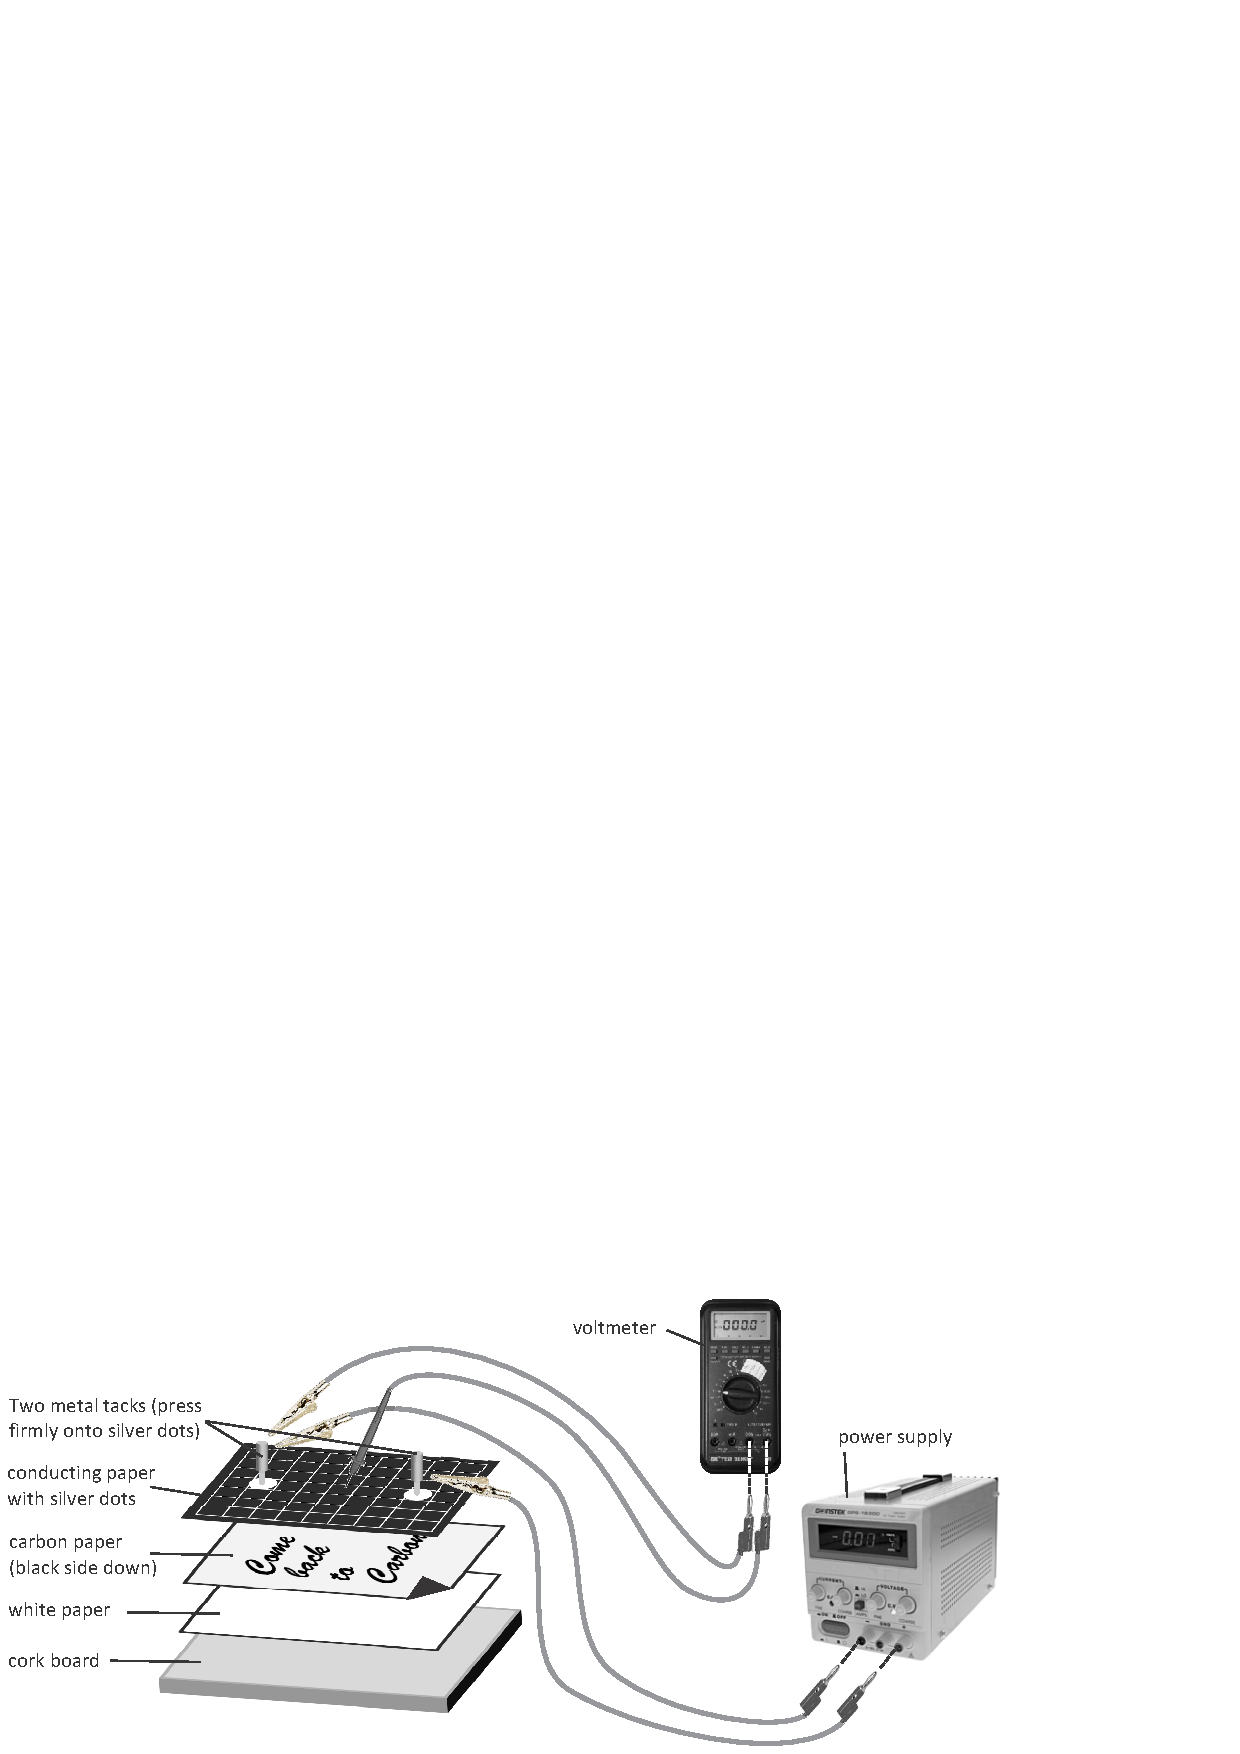
\includegraphics[scale=0.9]{electric_fields_and_equipotential_lines/apparatus_picture.pdf} \par}

%\medskip

\textbf{Introduction}

To help us understand electric forces, we can draw lines of electric field that start at positive charges (pointing directly away from them) and end at negative charges (pointing directly towards them).  


{\setlength{\columnsep}{0.4in}%
\begin{wrapfigure}[11]{r}{2.1in}
\vspace{-0.2in}
{\centering \includegraphics[width=1.7in]{electric_fields_and_equipotential_lines/field_and_potential.pdf} \par}

\textit{\small{A positive charge, with solid arrows showing electric field lines and dashed lines showing equipotentials.}}
\end{wrapfigure}

A charged particle moving along the direction of an electric field line gains or loses potential energy.  We also say that the \textit{electric potential} changes along a field line: the potential decreases going in the same direction as a field line, and the potential increases going in the opposite direction, against a field line.  But there is no change in electric potential in a direction \textit{perpendicular} to electric field lines; paths perpendicular to field lines are called \textit{equipotentials}.

\bigskip

\textbf{Experimental Setup}


Although it is difficult to measure electric field lines directly, you can measure differences in electric potential using a voltmeter.  In this lab, you will use a voltmeter to map out equipotential lines for different configurations of electric field lines.  

}%end of new columnsep

\begin{enumerate}[nosep]
\item Stack a piece of white paper, a piece of carbon paper, and a piece of special conducting paper with two round silver dots onto a cork board, as shown in the diagram above.
\item Push two metal thumbtacks HARD onto the silver dots, so the bottom of each tack is pressed firmly against the silver dot.
\item Use wire leads with alligator clips to connect the two tacks to the positive ($+$) and negative ($-$) terminals of the power supply.  Turn on the power supply and set it to an output of 20 volts.
\item Connect the negative input of the voltmeter (labeled ``COM'') to the same tack as the negative terminal of the power supply.  Connect the positive input of the voltmeter (labeled ``V-$\Omega$'') to the long plastic probe.  For details on how to use your voltmeter, see Appendix \ref{digital_multimeters}.
\end{enumerate}

\pagebreak[2]

\textbf{Activity 1: Field Lines for Two Point Charges}

\begin{enumerate}[labparts]
\item If you haven't already, set up the apparatus as just described.

\item \textit{Prediction:} Draw the electric field lines for two
oppositely charged point particles.  (Remember that field lines start at and point away from positive charges, and they terminate at and point towards negative charges.)  Also sketch the equipotential lines on your drawing, using dotted lines.
\answerspace{2in}

\item \textit{Now do the experiment!}  With your power supply set to 20 volts,
touch the conducting paper with the long probe on your voltmeter, and search around to find 
several points on 
paper registering 16 volts. (For more stable readings, hold the probe at an angle so that more area will be in contact with the conducting paper.)  When you find a place at 16 volts, push down or scratch a little bit 
so that the middle sheet of carbon paper will make marks on the bottom sheet of white paper---you 
can peak underneath to check.
\textit{You should be able to do this without puncturing the conducting paper.  Please don't poke holes, so the conducting paper can be reused!}

\item Repeat for 12 volts, 8 volts, and 4 volts.

\item You should end up with a series of dots on your sheet of paper. Connect
those associated with the same potential with smooth lines. Label each line 
with its associated voltage.  Attach a copy of the sheet with your measurements to this lab.
Draw a sketch of your results below.
\answerspace{2in}

\item Recalling the relationship between electric field lines and equipotential
lines, sketch in the electric field lines on the drawing you just made. 

\item Does your experimental result agree with your prediction? Explain.
\answerspace{1in}

\end{enumerate}

\pagebreak[2]
\textbf{Activity 2: Field Lines for Two Parallel Plates}

For static electric charges (when charges are not moving), the 
electric field within a conductor is zero, and electric field lines leave \textit{perpendicular} to a conductor's surface.  
In this activity, you will examine the field lines and equipotentials for two parallel conducting lines.  This situation is the two-dimensional analog of a pair of parallel conducting plates, also called a ``parallel plate capacitor.''

\begin{enumerate}[labparts]
\item \textit{Prediction:} Draw what you predict the field lines and equipotential
lines between two parallel plates will look like.
\answerspace{1.8in}

\item Set up your apparatus again, this time using the conducting paper with two silver parallel lines drawn on it.  Again, be sure to press the thumbtacks firmly down onto the silver conducting lines.  Carry out the instructions from Activity 1 to check your prediction above.  Attach a copy of the sheet with your measurements to this lab.
Draw a sketch of your results below, including equipotentials and field lines.
\answerspace{1.8in}

\item Does your result agree with your prediction? Explain.
\answerspace{.5in}

\end{enumerate}
\textbf{Activity 3: Field Lines Between a Point Charge and a Plate}

\begin{enumerate}[labparts]

\item Draw what you \textit{predict} the field lines and equipotential
lines between a point charge and a parallel plate will look like.
\answerspace{1.8in}

\item Map the field lines as before, attach a copy of the sheet with your measurements to this lab, and draw a sketch of your results below.
\answerspace{1.8in}

\item Does your result agree with your prediction? Explain.
\answerspace{.8in}

%\item If the potential is zero, must the electric field be zero as well?
%\answerspace{.3in}
%\item What can you say about the electric field along an equipotential line?\vspace{15mm}

\end{enumerate}
%\textbf{Activity 4: Field Lines for a Plate and a Charged Circle}

%\textbf{Prediction:} Sketch what you think the field and potential
%lines between a charged circle and a plate look like.
%\vspace{1in}

%\begin{enumerate}
%\item Determine the field lines.
%\item What is the field strength within a charged, continuous surface?\vspace{15mm}
%\end{enumerate}


\section{The Electric Field Near a Charged Rod}

\begin{comment}
This "lab" is by Matt Trawick.  I used this in my class for several years from an MS word file.  I converted it to latex and added it to the lab manual in 2015.  The figures could still be cleaned up a bit, but they work.
... and now I've cleaned up the figures too.
\end{comment}

\makelabheader %(Space for student name, etc., defined in master.tex)

\begin{wrapfigure}[10]{r}{0.385\textwidth}
\vspace{-.25in}
    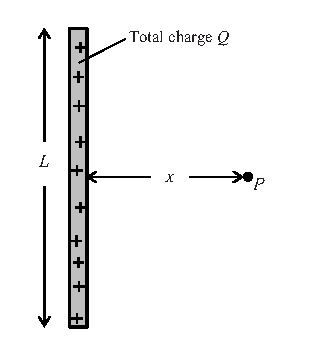
\includegraphics[width=0.3\textwidth]{electric_field_near_a_charged_rod/fig1.eps}
\end{wrapfigure}

\vspace{1cm}

\textbf{Objective and statement of the problem:}

Calculate the electric field $\vec{E}$ at a point $P$ a distance $x$ away from the midpoint of a thin rod
of length $L$ and total charge $Q$.

\vspace{1cm}

\textbf{Introduction and outline of solution:}

Think of the rod as a bunch of teeny-tiny little point charges $dQ$ arranged in a row. You will solve this problem by calculating the sum (actually an integral) of the electric fields due to each point charge.  In the second figure, below, we have added a set of coordinate axes, and defined a tiny bit of charge $dQ$ that is on a tiny bit of length $dy$.  
\par

\begin{wrapfigure}[6]{r}{0.4\textwidth}
%\vspace{-23pt}
\vspace{-.65in}
   \includegraphics[width=0.4\textwidth]{electric_field_near_a_charged_rod/fig2.eps}
\end{wrapfigure}

%\vspace{0.1cm}
%{\centering \resizebox*{0.5\textwidth}{!}{\includegraphics{electric_field_near_a_charged_rod/fig2.eps}} \par}

\par
\vspace{0.5cm}
\par
\textbf{Step 1:} \newline
In words, what is the direction of the electric field at point $P$ due to just one little bit of charge $dQ$ shown?

\vspace{.6in}

What is the direction of the electric field at point $P$ due to the whole rod?

\vspace{.6in}

\textbf{Step 2:} \newline
What is the magnitude of the electric field $|d\vec{E}|$  due to just the bit of charge $dQ$?  (Write the relevant distance in terms of $x$ and $y$.)
\[
|d\vec{E}|=\hspace{0.7in}
\]
\vspace{.3in}

\textbf{Step 3:} \newline
What is the magnitude of the $x$-component of   $d\vec{E}$?  (It's similar to your answer above but with an extra $\sin \theta$ or $\cos \theta$.) 
\[
d\vec{E}_x=\hspace{1in}
\]
\vspace{.3in}

\pagebreak
\textbf{Step 4:} \newline
Rewrite the last step, giving  $\sin \theta$ or $\cos \theta$ in terms of a ratio involving $x$, $y$, and/or $\sqrt{x^2 + y^2}$.
\[
d\vec{E}_x=\hspace{1in}
\]
\vspace{.3in}

\textbf{Step 5:} \newline
The linear charge density $\lambda$ of the rod is given by $\lambda = Q/L$.  Write $dQ$ in terms of $\lambda$  and $dy$, then in terms of $Q$, $L$ and $dy$.
\[
dQ=\hspace{0.7in}=\hspace{0.7in}
\]
\vspace{.3in}

\textbf{Step 6:} \newline
Combine your answers to steps 4 and 5 to write $\vec{E}$ as a single integral over $dy$ which you can solve.  What are the limits of the integral?
\[
\vec{E}=\int d\vec{E}_x=\hspace{1.5in}
\]
\vspace{.3in}

\textbf{Step 7:} \newline
Evaluate the integral.  
\[
\vec{E}=\hspace{2in}
\]

 \vspace{3in}

\textit{Note: one of the following might be helpful:}
\begin{flalign*}
& \int \! \frac{1}{\left (y^2 + a^2 \right )^\frac{3}{2}} \, dy=\frac{y}{a^2 \sqrt{y^2 + a^2}} &\\
& \int \! \frac{y}{\left (y^2 + a^2 \right )^\frac{3}{2}} \, dy=\frac{-1}{\sqrt{y^2 + a^2}} \\
& \int \! \frac{1}{y^2 + a^2} \, dy=\frac{1}{a} \tan^{-1} \frac{y}{a}
\end{flalign*}
%\]


\section{An Example Problem Using Electric Potential}

\begin{comment}
This lab is really just a worksheet I've used in my 132 class. --Matt Trawick, 6/2015
\end{comment}

\makelabheader %(Space for student name, etc., defined in master.tex)

\vspace{0.1in}
\textbf{Objective and Statement of Problem:}
 
An ionized helium atom (mass $m=6.7\times 10^{-27}$~kg, charge $q_0=+1.6\times 10^{-19}$~C) is released from rest 20~cm away from a +60~nC point charge.  What is the helium ion's speed $v$ when it is 60~cm away from the point charge?

\textbf{Solution:}

Your first instinct might be to find the force on the helium ion, and then get the acceleration and velocity from there.  But that would be hard, because the force is different everywhere, leading to an acceleration that is not constant.  It's much easier to use the idea of electric potential and conservation of energy!

\answerspace{0.1in}

\textbf{Step 1:} 

Find the electric potential $V_i$ at the place 20~cm from the point charge, and $V_f$ at 60~cm from the point charge.  (Your answers should be in volts.)
\answerspace{1.9in}


\textbf{Step 2:}

Use the idea of conservation of energy to write the final kinetic energy of the helium ion $K_f$ in terms of its charge $q_0$ and the potential difference $V_f-V_i$.  What is your numerical answer, in Joules?
\vspace{1.6in}

\textbf{Step 3:}

So what's the final speed of the helium ion, in meters per second?
\answerspace{1.4in}


\section{The Electric Potential\footnote{%
1990-93 Dept. of Physics and Astronomy, Dickinson College. Supported
by FIPSE (U.S. Dept. of Ed.) and NSF. Portions of this material may
have been modified locally and may not have been classroom tested
at Dickinson College.
}}

\makelabheader %(Space for student name, etc., defined in master.tex)

\bigskip
\textbf{Overview}

It takes work to lift an object in the Earth's gravitational field.
Lowering the object releases the energy that was stored as potential
energy when it was lifted. Last semester, we applied the term \emph{conservative}
to the gravitational force because it {}``releases'' \emph{all}
of the stored energy. We found experimentally that the work required
to move a mass in the gravitational field was path independent. This
is an important property of any conservative force. Given the mathematical
similarity between the Coulomb force and the gravitational force,
it should come as no surprise that experiments confirm that an electric
field is also conservative. This means that the work needed to move
a charge from point $A$ to point $B$ is independent of the path taken
between points. A charge could be moved directly between the two points
or looped around and the work expended to take either path would be
the same. Work done by an electric field on a test charge $q$ traveling
between points $A$ and $B$ is given by
\begin{equation*}
W=\int ^{B}_{A}  \vv{F}\cdot \vv{ds}=\int ^{B}_{A}q\vv{E}\cdot \vv{ds} 
\end{equation*}

\bigskip
\textbf{Activity 1: Work Done on a Charge Traveling in a Uniform Electric
Field}

(a) A charge $q$ travels a distance $d$ from point $A$ to point $B$; the path
is parallel to a uniform electric field of magnitude $E$. What is the
work done by the field on the charge? How does the form of this equation
compare to the work done on a mass $m$ traveling a distance $d$ in the
almost uniform gravitational field near the surface of the Earth?

\vspace{0.3cm}
{\centering \resizebox*{0.2\textwidth}{!}{\includegraphics{electric_potential/electric_potential_fig_1.eps}} \par}
\answerspace{0.3cm}

(b) The charge $q$ travels a distance $d$ from point $A$ to point $B$ in a
uniform electric field of magnitude $E$, but this time the path is perpendicular
to the field lines. What is the work done by the field on the charge?

\vspace{0.3cm}
{\centering \resizebox*{0.2\textwidth}{!}{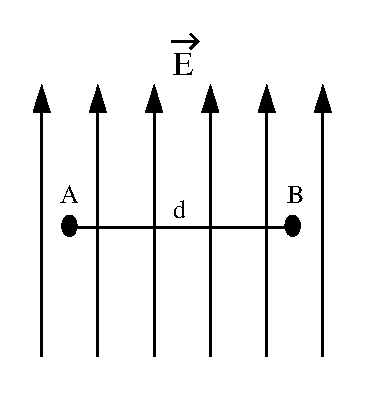
\includegraphics{electric_potential/electric_potential_fig_2.eps}} \par}
\answerspace{0.3cm}

\pagebreak[2]
(c) The charge $q$ travels a distance $d$ from point $A$ to point $B$ in a
uniform electric field of magnitude $E$. The path lies at a $45^{\circ}$~angle 
to the field lines. What is the work done by the field on the
charge?

\vspace{0.3cm}
{\centering \resizebox*{0.2\textwidth}{!}{\includegraphics{electric_potential/electric_potential_fig_3.eps}} \par}
\answerspace{0.5cm}

\textbf{Potential Energy and Potential Difference}

Recall that by definition the work done by a conservative force equals
the negative of the change in potential energy, so that the change
in potential energy of a charge moving from point $A$ to point $B$ under
the influence of an electrical force is given by:
\begin{equation*}
\Delta U=U_{B}-U_{A}=-\int ^{B}_{A}q\vv{E}\cdot \vv{ds}
\end{equation*}

By analogy to the definition of the electric field, we are interested
in defining the \emph{electric potential difference} $\Delta V=V_{B}-V_{A}$
as the change in electric potential energy $\Delta U$ per
unit charge. Formally, \emph{the potential difference is defined as
the work per unit charge that an external agent must perform to move
a test charge from $A$ to $B$ without changing its kinetic energy}. The
potential difference has units of joules per coulomb. Since 1~J/C
is defined as one \emph{volt}, the potential difference is often referred
to as \emph{voltage}.

\textbf{Activity 2: The Equation for Potential Difference}

Write the equation for potential difference as a function of $\vv{E}$,
$\vv{ds}$, $A$, and $B$.
\answerspace{15mm}

\textbf{The Potential Difference for a Point Charge}

The simplest charge configuration that can be used to consider how
voltage changes between two points in space is a single point charge.
We will start by considering a single point charge and then move on
to more complicated configurations of charge.

A point charge $q$ produces an electric field that points radially outward
in all directions for a positive charge, radially inward for a negative charge. The line integral equation for the potential difference
can be evaluated to find the potential difference between any two
points in space $A$ and $B$ (a line integral is one that follows a path
through space).

It is common to choose the reference point for the determination of
voltage to be set at infinity so that we are determining the work
per unit charge that is required to bring a test charge from infinity
to a certain point in space. Let's choose a coordinate system so that
the point charge is conveniently located at the origin. In this case
we will be interested in the potential difference between infinity
and some point which is a distance $r$ from the point charge. Thus,
we can write the equation for the potential difference, or voltage,
as
\begin{equation*}
\Delta V=V_{B}-V_{A}=V_{r}-V_{\infty }=-\int ^{r}_{\infty} \vv{E}\cdot \vv{ds}
\end{equation*}

Often, when the reference point for the potential difference is at
infinity, this difference is simply referred to as ``the potential'',
and the symbol $\Delta V$ is just replaced with the symbol $V$.

\pagebreak[2]
\textbf{Activity 3: Potential at a Distance r from a Charge}

Starting from the expression for the electric field of a point charge,
show that, if $A$ is at infinity and $B$ is a distance $r$ from a point
charge $q$, then the potential $V$ is given by the expression
\begin{equation*}
V=\frac{k_eq}{r}
\end{equation*}
where $k_e=\frac{1}{4\pi \varepsilon _{\circ }} = 8.99 \times 10^{9} \ \mathrm{N\cdot m}^2
/ \mathrm{C}^2 .$
\textbf{Hint:} What is the mathematical expression for an $E$-field
from a point charge?

%\vspace{0.3cm}
%{\centering \resizebox*{0.4\textwidth}{!}{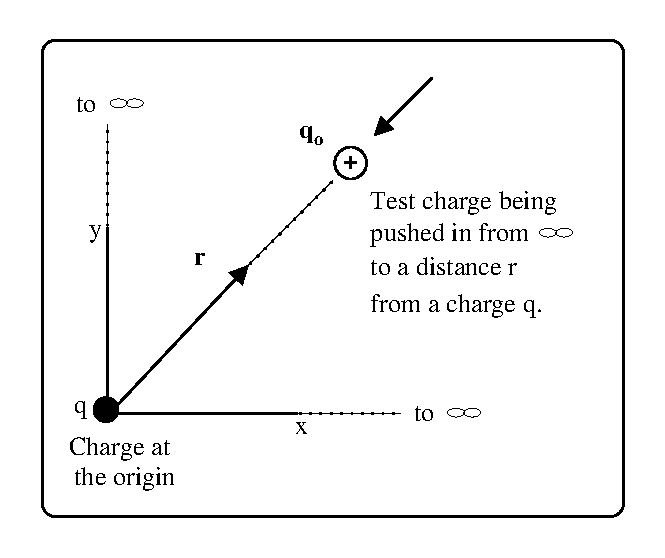
\includegraphics{electric_potential/electric_potential_fig_4.eps}} \par}
{\resizebox*{0.4\textwidth}{!}{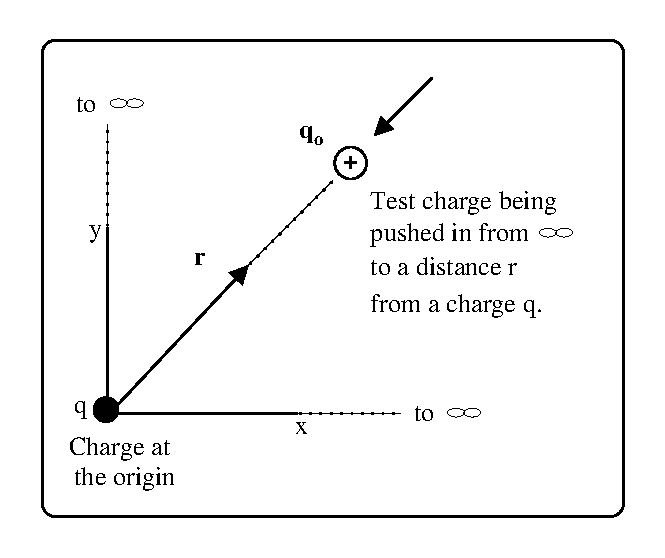
\includegraphics{electric_potential/electric_potential_fig_4.eps}} \par}
%\vspace{0.3cm}

\answerspace{15mm}

\textbf{Activities 4 and 5: Potential Due to Continuous Charge Distributions}

The potential from a continuous charge distribution can be calculated
several ways. Each method should yield approximately the same result.
First, we can use an integral method in which the potential $dV$ from
each element of charge $dq$ is integrated mathematically to give a total
potential at the location of interest. Second, we can approximate
the value of the potential $V$ by summing up several finite elements
of charge \( \Delta q \) by using a computer spreadsheet or hand
calculations.

Again, let's consider a relatively simple charge distribution. In
this case we will look at a ring with charge uniformly distributed
on it. We will calculate the potential on the axis passing through
the center of the ring as shown in the diagram below. (Later on you
could find the potential difference from a disk or a sheet of charge
by considering a collection of nested rings).

\vspace{0.3cm}
{\centering 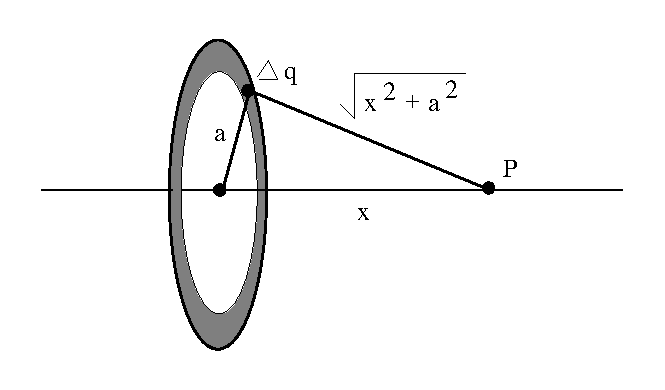
\includegraphics[scale=0.8]{electric_potential/electric_potential_fig_5.eps} \par}
\vspace{0.3cm}

\vspace{2in}
A ring of charge has a total charge of $Q = 20\ \mu$C (i.e. $20
\times 10^{-6}$~C). The radius of the ring, $a$, is 30~cm. We want
to find the electric field and the electric potential at a distance $x$ from the ring along an axis that is perpendicular to the ring
and passes through its center. Let's begin by calculating the potential
in the next activity.

\textbf{Hints:} Since the potential is a scalar and not a vector we
can calculate the potential at point $P$ (relative to $\infty$)
for each of the charge elements $\Delta q$ and add them to each
other. This looks like a big deal but it is actually a trivial problem
because all the charge elements are the same distance from point $P$.

\textbf{Activity 4: Numerical Estimate of the Potential due to a Charged
Ring}

(a) Divide the ring into 20 elements, each of charge $\Delta q = 1.0 \times 10^{-6}$~C and
calculate the total $V$ at a distance of $x = 20$~cm from the center of
the ring using a spreadsheet program or by hand calculation. Summarize
the result below. Be sure to attach a printout of your spreadsheet
results if your instructor wants it.
\answerspace{1.25in}

\textbf{Activity 5: Calculation of the Potential due to a Charged Ring}

By following the steps below, you can use an integral to find a more
exact value of the potential.

(a) Show that 
\begin{displaymath}
V=k_e\int \frac{dq}{r}=k_e\int \frac{dq}{\sqrt{x^{2}+a^{2}}}
\end{displaymath}
\answerspace{20mm}

(b) Explain why
\begin{displaymath}
 k_e\int \frac{dq}{\sqrt{x^{2}+a^{2}}}=\frac{k_e}{\sqrt{x^{2}+a^{2}}}\int dq
\end{displaymath}
(That is, explain why $\sqrt{x^{2}+a^{2}}$ can be pulled out of the integral).
\answerspace{20mm}

(c) Perform the integration in part (b) above. Then substitute values
for $a$, $x$, and $Q$ into the resulting expression in order to obtain a
more {}``exact'' value for the potential.
\answerspace{25mm}

(d) How does the {}``numerical'' value that you obtained in Activity
4 compare with the {}``exact'' value you obtained in (c)?
\answerspace{10mm}

\pagebreak[2]
\textbf{Activity 6: \( \Delta  \)V from a Ring Using the E-field Method}

Now let's take a completely different approach to the same problem.
If we can find the vector equation for the electric field at point
$P$ due to the ring of charge, then we can use the expression
\begin{equation}
\Delta V=V_{r}-V_{\infty }=-\int ^{r}_{\infty }\vv{E}\cdot \vv{ds} 
\end{equation}
as an alternative way to find a general equation for the potential
at point $P$.

%\answerspace{0.3cm}
{\centering \includegraphics[scale=0.8]{electric_potential/electric_potential_fig_6.eps} \par}
%\answerspace{0.3cm}


(a) Starting from the electric field of a point charge, show that
the electric field at point $P$ from the charged ring is given by
\begin{equation*}
\vv{E}=\frac{k_eqx}{(x^{2}+a^{2})^{3/2}}\hat{x} .
\end{equation*}
\textbf{Hints:} (1) Why is there no $y$ component of the $E$-field? (2)
$\cos \theta =\frac{x}{\sqrt{x^{2}+a^{2}}}$
\answerspace{30mm}

(b) Use equation (1) above, and your result from (a) to find $\Delta V$.  \textbf{Hint:} You will probably need to consult the integral tables in the appendix of your text.
\textbf{Note:} The above expression for $\vv{E}$ is only valid along the $x$-axis.
\answerspace{30mm}

(c) How does the result compare to that obtained in Activity 5(c)?
\answerspace{10mm}

\pagebreak[2]
\textbf{Activity 7: Sketches of Electric Field Lines and Equipotentials}

Sometimes it is possible to move along a surface without doing any
work. Thus, it is possible to remain at the same potential energy
anywhere along such a surface. If an electric charge can travel along
a surface without doing any work, the surface is called an \emph{equipotential
surface}.
Consider the three different charge configurations shown below. Where
are the equipotential surfaces? What shapes do they have?

\textbf{Hint:} If you have any computer simulations available to you
for drawing equipotential lines associated with electrical charges,
you may want to check your guesses against the patterns drawn in one
or more of the simulations.

(a) Suppose that you are a test charge and you start moving at some
distance from the charge below (such as 4~cm). What path could you
move along without doing any work, i.e. $\vv{E}\cdot \vv{ds}$
is always zero? What is the shape of the equipotential surface? Remember
that in general you can move in \emph{three} dimensions.

%\vspace{0.3cm}
{\centering \resizebox*{0.27\columnwidth}{!}{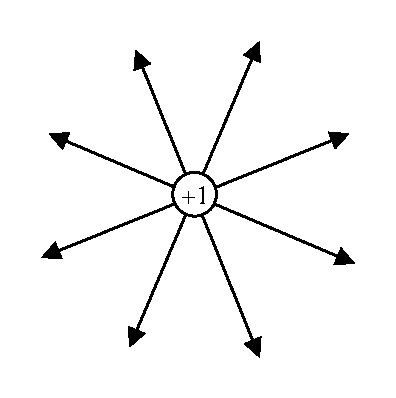
\includegraphics{electric_potential/electric_potential_fig_7.eps}} \par}
%\vspace{0.3cm}

(b) Find some equipotential surfaces for the charge configuration
shown below, which consists of two charged metal plates placed parallel
to each other. What is the shape of the equipotential surfaces?

%\vspace{0.3cm}
{\centering \resizebox*{0.26\textwidth}{!}{\includegraphics{electric_potential/electric_potential_fig_8.eps}} \par}
%\vspace{0.3cm}

(c) Find some equipotential surfaces for the electric dipole charge
configuration shown below.

\vspace{0.3cm}
{\centering \resizebox*{0.24\textwidth}{!}{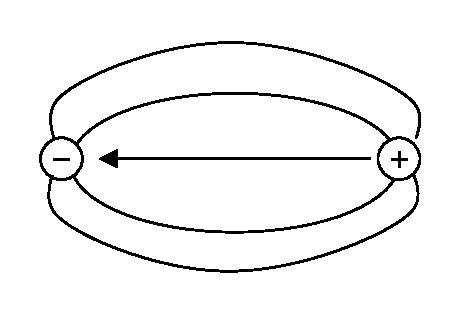
\includegraphics{electric_potential/electric_potential_fig_9.eps}} \par}
\vspace{0.3cm}

(d) In general, what is the relationship between the direction of
the equipotential lines you have drawn (representing that part of
the equipotential surface that lies in the plane of the paper) and
the direction of the electric field lines?
\answerspace{10mm}



\section{Finding Potential from the Electric Field}

\begin{comment}
This lab was originally written by Matt Trawick in spring 2015.  I found that students are really terrible at figuring out potential from electric field, and especially the idea of a reference potential.  The goal of this lab is to help them get better at this.  
\end{comment}

\makelabheader %(Space for student name, etc., defined in master.tex)

\vspace{0.4in}
\textbf{Introduction:}

In this lab, you will calculate and graph the electric potential $V$ from a known electric field $E$.  Keep in mind that the relationship between these two can be written as either a definite or indefinite integral:
\begin{displaymath}
\Delta V_{AB} = -\int_A^B{\vec{E} \cdot \vec{ds}} \qquad \textrm{ or } \qquad
V =-\int{\vec{E} \cdot \vec{ds}} 
\end{displaymath}
When evaluating the indefinite integral, remember that you always need a constant of integration, $+C$.  
\vspace{0.4in}

\begin{wrapfigure}[5]{r}{0.35\textwidth}
%\vspace{-0.2 in}
%    \includegraphics[width=0.4\textwidth]{finding_v_from_e/fig1.eps}
\hspace*{\fill}
\begin{lab_axis}[lab_grid,
	scale only axis = true,
	width={1.5in}, height={1.2in},
	xmin=0, xmax=3,
	ymin=-1, ymax=6,
	ylabel = {Field $E$ (N/C)},
	ytick = {-5,0,5,10},
	minor y tick num=4,
	minor x tick num=1,
	xlabel = {$x$ (m)},
	y0_line,
]
\addplot coordinates {(0,5) (2,5) (2,0) (3,0) };
\end{lab_axis}
\end{wrapfigure}

\textbf{Activity 1} 

The graph to the right shows a region of a uniform electric field $E(x)$.  

(a) If a positively charged particle starts at $x=0$ and is accelerated by the electric field to $x=2$, would the particle's kinetic energy $K$ \textit{increase} or \textit{decrease}?
\answerspace{0.7in}

(b) In part (a), would the particle's potential energy $U$ \textit{increase} or \textit{decrease}?
\answerspace{0.7in}

(c) Calculate the change in electric potential $\Delta V$ from $x=0$ to $x=2$. (Careful with your signs!)
\answerspace{0.9in}

(d) If the potential at the origin is defined as $V(0)=0$ volts (our ``reference''), what is the value of the potential $V$ at $x=2$?
\answerspace{0.7in}

\pagebreak
(e) Draw a graph of the electric potential on the axes below.  Include a scale on the vertical axis.
%\begin{center}
%\includegraphics[width=0.4\textwidth]{finding_v_from_e/fig2.eps}
%\end{center}

\begin{lab_axis}*[lab_grid,
	scale only axis = true,
	width={3.0in}, height={1.5in},
	xmin=0, xmax=3,
	ymin=-4, ymax=4,
	ylabel = {Electric potential $V$},
	xlabel = {$x$ (m)},
	yticklabels = { , , },
	y0_line,
]
\end{lab_axis}

(f) Calculate the change in electric potential $\Delta V$ between $x=2$ and $x=3$.
\answerspace{0.5in}

(g) Recalling your answers to parts (d) and (f), what is the value of the electric potential $V$ at $x=3$?  (After you've answered this, you may want to go back and fix up your graph in part (e) to clarify $V(x)$ for $x>2$.
\answerspace{0.5in}

(h) Draw a graph showing the potential if we chose our reference so that $V(\infty)=0$ instead.  
%\begin{center}
%\includegraphics[width=0.4\textwidth]{finding_v_from_e/fig2.eps}
%\end{center}

\begin{lab_axis}*[lab_grid,
	scale only axis = true,
	width={3.0in}, height={1.5in},
	xmin=0, xmax=3,
	ymin=-4, ymax=4,
	ylabel = {Electric potential $V$},
	xlabel = {$x$ (m)},
	yticklabels = { , , },
	y0_line,
]
\end{lab_axis}

(i) Write an equation describing $V(x)$ based on your graph above.
\begin{displaymath}
V(x) = \begin{cases}
        \rule{1.3in}{0in}  & \textrm{when } 0<x<2\\
        \\
        \hspace{1.3in} & \textrm{when }  2 < x
        \end{cases}
\end{displaymath}
\answerspace{0.1in}

\pagebreak
\begin{wrapfigure}[5]{r}{0.5\textwidth}
%\vspace{-0.2 in}
%    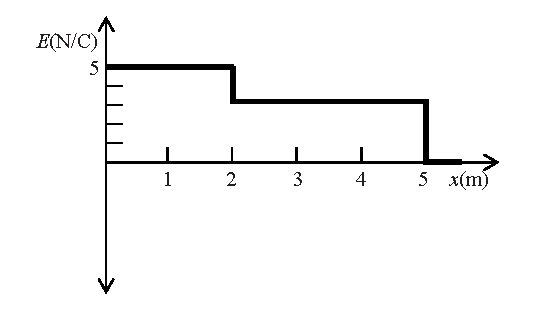
\includegraphics[width=0.5\textwidth]{finding_v_from_e/fig3.eps}
\hspace*{\fill}
\begin{lab_axis}[lab_grid,
	scale only axis = true,
	width={2.5in}, height={1.2in},
	xmin=0, xmax=6,
	ymin=-1, ymax=6,
	ylabel = {Field $E$ (N/C)},
	ytick = {-5,0,5,10},
%	ytick distance = 5,
	minor y tick num=4,
	xlabel = {$x$ (m)},
	y0_line,
]
\addplot coordinates {(0,5) (2,5) (2,3) (5,3) (5,0) (6,0)};
\end{lab_axis}
\end{wrapfigure}

\textbf{Activity 2} 

The graph to the right shows the electric field $E(x)$ in some other region.
(a) Calculate the change in electric potential $\Delta V$ between $x=0$ and $x=2$.
\answerspace{0.8in}

(b) Calculate the change in electric potential $\Delta V$ between $x=2$ and $x=5$.
\answerspace{0.7in}

(c) Draw a graph showing the potential, where the reference is $V(\infty)=0$.
%\begin{center}
%\includegraphics[width=0.45\textwidth]{finding_v_from_e/fig4.eps}
%\end{center}

\begin{lab_axis}*[lab_grid,
	scale only axis = true,
	width={3.0in}, height={1.8in},
	xmin=0, xmax=6,
	ymin=0, ymax=10,
	ylabel = {Electric potential $V$},
	xlabel = {$x$ (m)},
	ytick distance = 2,
	yticklabels = { , , },
	y0_line,
	minor tick num=1,
]
\end{lab_axis}


(d) Use the indefinite integral $V =-\int{\vec{E} \cdot \vec{ds}}$  to write an equation for $V(x)$ in the region $2<x<5$.  (Remember to include an integration constant, $+C$.  What equation should you use to find the value of $C$?)
\answerspace{1.0in}


(e) Write an equation describing $V(x)$ for all $x>0$.  It will be of the form
\begin{displaymath}
V(x) = \begin{cases}
        blah \, blah \, blah  & \textrm{when } 0<x<2\\
        yada \, yada \, yada & \textrm{when }  2<x<5\\
        something \, else & \textrm{when }  5 < x
        \end{cases}
\end{displaymath}

\answerspace{1.1in}

\pagebreak[2]
\textbf{Activity 3} 

The graph below shows the electric field $E(x)$ in yet another region.
%\begin{center}
%\includegraphics[width=0.6\textwidth]{finding_v_from_e/fig5.eps}
%\end{center}

\begin{lab_axis}*[lab_grid,
	scale only axis = true,
	width={3.5in}, height={1.7in},
	xmin=0, xmax=8,
	ymin=-6, ymax=6,
	ylabel = {Electric field $E$ (N/C)},
%	ytick = {-10,-5,0,5,10},
	ytick distance = 2,
	minor y tick num=1,
	xlabel = {$x$ (m)},
	y0_line,
]
\addplot coordinates {(0,-5) (2,-5) (2,0) (4,0) (4,3) (7,3) (7,0) (8,0)};
\end{lab_axis}

(a) Calculate the change in electric potential $\Delta V$ over each of the three regions shown.
\vspace{1.2in}

(b) Draw a graph of the potential $V(x)$, where the reference is $V(\infty)=0$.

\begin{lab_axis}*[lab_grid,
	scale only axis = true,
	width={3.5in}, height={1.5in},
	xmin=0, xmax=8,
	ymin=-4, ymax=4,
	ylabel = {Electric potential $V$},
	xlabel = {$x$ (m)},
	yticklabels = { , , },
	y0_line,
]
\end{lab_axis}

%\begin{center}
%\includegraphics[width=0.6\textwidth]{finding_v_from_e/fig6.eps}
%\end{center}

(c) Is $V=0$ at $x=3$ (bearing in mind that the correct answer is ``No'')?
\answerspace{0.5in}

(d) In general, if $E=0$, does it follow that $V=0$?
\answerspace{0.5in}

(e) Where on your graph does $V=0$?  In general, if $V=0$, does it follow that $E=0$?
\answerspace{0.5in}

\pagebreak[2]
\begin{wrapfigure}[6]{r}{0.4\textwidth}
%\vspace{0.2 in}
%    \includegraphics[width=0.4\textwidth]{finding_v_from_e/fig7.eps}
\hspace*{\fill}
\begin{lab_axis}[lab_noticks_2quads,
	scale only axis = true,
	algebraic_labels,
	width={2.2in}, height={1.3in},
	ymin=-0.3, ymax=1.5,
	xmin= 0, xmax = 4,
	ylabel = {$E$},
	xlabel = {$r$},
	xtick = {1},
	xticklabel = {$R$},
]
\addplot +[domain= 0 : 1] {x};
\addplot +[domain= 1 : 3.8] {1/x^2};
\end{lab_axis}
\end{wrapfigure}

\textbf{Activity 4} 

The graph to the right shows the electric field $E(r)$ near a uniformly charged sphere of radius $R$.  The electric field is given by
\begin{displaymath}
E(r) = \begin{dcases}
        \frac{k_eQr}{R^3}  &  0<r<R\\
        \frac{k_eQ}{r^2}  &  R<r
        \end{dcases}
\end{displaymath}

%(a) Use a definite integral to calculate $\Delta V$  between $r=R$ and $r=\infty$.
%\vspace{1.1in}

%(b) Use a definite integral to calculate $\Delta V$ between $r=0$ and $r=R$.
%\vspace{1.1in}

%Removed these last two parts, 2/14/2015. --MT.  These questions hurt more than they helped; students were trying to use the results of the definite integrals to figure out the constants of integration.  No big loss; it's not like this lab was too short before

%\vspace{0.5in}

(a) Draw a graph of the potential $V(r)$, using $V(\infty)=0$ as a reference.  (Hints: try telling yourself a story about how much potential energy you'd be adding to the system if you used your hand to push a small positive particle in from $r=\infty$.  Also remember that $E = - \frac{dV}{dr}$.  If you're not sure, sketch your best guess with a dotted line and go on to the next question.)
%\begin{center}
%\includegraphics[width=0.5\textwidth]{finding_v_from_e/fig8.eps}
%\end{center}

\begin{lab_axis}*[lab_noticks_2quads,
	scale only axis = true,
	algebraic_labels,
	width={2.8in}, height={1.8in},
	xmin= 0, xmax = 4,
	ylabel = {$V$},
	xlabel = {$r$},
	xtick = {1},
	xticklabel = {$R$},
]
\end{lab_axis}

(b) Use indefinite integrals to write equations for $V(r)$ for each of the two regions, using $V(\infty)=0$ as your reference.  Be careful with signs, and remember the integration constants!
\answerspace{1.3in}

\vfill
(c) Now that you've calculated $V(r)$ exactly, go back and look at your graph in part (a).  Are your answers consistent?

	\include{electric_field_and_electric_potential/EF_EP_1}
	
\section{The Electric Field and the Electric Potential II}

\makelabheader %(Space for student name, etc., defined in master.tex)

\textbf{Objective}

\begin{itemize}
\item To investigate the electric field and potential of a charge distribution.
\end{itemize}

\textbf{Apparatus}

\begin{itemize}
\item Electric field and potential simulation entitled {\it EMField}.
\end{itemize}

\textbf{Introduction}

In the previous unit (which we will refer to as Investigation 1) we studied the dependence
of the electric field and the electric potential on $r$, the distance from a
single charge.
Now we will study the same ideas for a different charge distribution.

\textbf{Investigation 2: Four Symmetrically Arranged Charges}

\textbf{Activity 1: The Electric Field}

(a) Go to \filename{Start $\rightarrow$ Programs $\rightarrow$ Physics Applications} and open the program \filename{EMField}.
(Or, if it's already running, use the options under the 
\textbf{Display} menu to clear the table top and delete any charges.)
Go to the \textbf{Sources} menu and select \textbf{3D Point Charges}.
A blank `table top' with a set of menu 
buttons at the top and bottom will appear (see Figure 1 in Investigation 1, the previous unit).

(b) Go to the \textbf{Display} menu and set {\it EMField} to
{\bf Show Grid} and {\bf Constrain to Grid} if they are not already set.
These choices will make the following investigation a bit easier to perform.

(c) Under \textbf{Sources}, click on \textbf{3D Point Charges}. Select the
charge labeled {}``+4'' from the available set by clicking on it.
Add four individual charges, arranging them symmetrically within about
1 cm of the central point where the {}``+4'' charge was located
in Investigation 1 (the previous unit). 

(d) {\bf Prediction:} How will the electric field be oriented within the region of the four charges?
How will the field be oriented outside the region of the four charges?
How will the field depend on $r$, the distance from the center of the four charges, at large $r$?
\answerspace{25mm}

(e) Click anywhere in the table top and you will see an arrow drawn.
The size and direction of the arrow represent the magnitude and direction of
the electric field at that point due to the four charges.
In what direction does the arrow point?
Click on the opposite side of the table top.
In what direction does this arrow point? How is it related to the first arrow?
\answerspace{15mm}

(f) Click on many points so that you get a wide range of magnitudes from large
(barely fits on the table top) to small (barely bigger than a dot).

\pagebreak[2]
(g) Print the table top and use a ruler to measure the lengths of each of the arrows on your plot, for points \textbf{outside} the region of the four charges. Enter this data in the following table. Use the scale at the bottom of the table top to convert the length of each arrow into an electric field magnitude.
The units of the scale electric field vector are $1.0 ~ N/C$.

\vspace{0.3cm}
{\centering \begin{tabular}{|c|c|c|}
\hline 
~~~Distance from Charge Center (cm)~~~&
~~~Arrow Length (cm)~~~&
~~~Measured E (N/C)~~~\\
\hline
\hline 
&
&
\\
\hline 
&
&
\\
\hline 
&
&
\\
\hline 
&
&
\\
\hline 
&
&
\\
\hline 
&
&
\\
\hline 
&
&
\\
\hline 
&
&
\\
\hline 
&
&
\\
\hline
\end{tabular}\par}
\vspace{0.3cm}


(h) \textbf{Prediction}: From Coulomb's Law, we expect the spatial variation
of the field strength to obey a power law: \( \left| E\right| =Ar^{n} \),
where \( A \) and \( n \) are constants. What do you predict the
value of \( n \) to be?
\answerspace{15mm}

(i) Graph your results. Using the power fitting
function, determine the power of the function, $n$, and record it here.
Attach the plot to this unit.
\answerspace{15mm}

(j) Does your result agree with your prediction? Explain any discrepancy.\vspace{15mm}

\textbf{Activity 2: The Electric Potential}

(a) Under the {\bf Display} menu click on {\bf Clean up Screen} to erase the
electric field vectors.

(b) \textbf{Prediction}: You will now take measurements of the potential.
How do you expect the electric potential to change with distance from the center of the four charges?
\answerspace{15mm}
 
(c) Click on the \textbf{Potential} option under the \textbf{Field and Potential} menu. Click on the table top and a marker will be
placed at that point and labeled with the value of the potential there.
Click on many spots on the table top from very close to the charges to
far away.
When you are finished print the table top.
\answerspace{15mm}

\pagebreak
(d) Measure and record in the following table the values of the distance from the center of the point charge region (for points outside the region of the four charges) and the potential.

\vspace{0.3cm}
{\centering \begin{tabular}{|c|c|c|}
\hline 
~~~Distance from Charge Center (cm)~~~&
~~~Measured V (volts)~~~\\
\hline
\hline 
&
\\
\hline 
&
\\
\hline 
&
\\
\hline 
&
\\
\hline 
&
\\
\hline 
&
\\
\hline 
&
\\
\hline 
&
\\
\hline 
&
\\
\hline
\end{tabular}\par}
\vspace{0.3cm}


(e) \textbf{Prediction}: From Coulomb's Law and the definition of the
electric potential, we expect the spatial variation of the potential
to obey a power law: \( \Delta V=Br^{m} \), where \( B \)
and \( m \) are constants. What do you predict the value of \textbf{\( m \)}
to be?\vspace{20mm}


(f) Graph your results. Using the power fitting
function, determine the power of the function, $m$, and record it here.
\vspace{20mm}

(g) Does your result agree with your prediction? Explain any discrepancy.\vspace{20mm}

(h) How do your results for the power constants, $n$ and $m$, of the four
symmetrically-arranged charges compare with the power constants you
determined in Investigation 1 (the previous unit) for the single point charge?\vspace{20mm}

(i) What can you conclude about the field and potential effects due to
a distribution of charge outside the region of the distribution (in
relation to a single point charge)?


	
\section{The Electric Field and the Electric Potential III}

Name \rule{2.0in}{0.1pt}\hfill{}Section \rule{1.0in}{0.1pt}\hfill{}Date
\rule{1.0in}{0.1pt}

\textbf{Objective}

\begin{itemize}
\item To investigate the relationship between the electric potential and
the electric field.
\end{itemize}

\textbf{Apparatus}

\begin{itemize}
\item Electric field and potential simulation entitled {\it EM Field 6}.
\end{itemize}

\textbf{Introduction}

In the previous units (which we will refer to as Investigation 1 and 2) we studied the dependence
of the electric field and the electric potential on $r$, the distance from
a charge distribution.
Now we will study the same ideas for a charge distribution commonly found in physics and chemistry
using the same methods we used before.

\textbf{Investigation 3: An Electric Dipole}

\textbf{Activity 1: The Electric Field}

(a) Start the program {\it EM Field 6} from the 132 menu or use the options under the 
\textbf{Display} menu to clear the table top and delete any charges.
Go to the \textbf{Sources} menu and select \textbf{3D Point Charges}.
A blank `table top' with a set of menu 
buttons at the top and bottom will appear.

(b) Go to the Display menu and set {\it EM Field 6} to
{\bf Show Grid} and {\bf Constrain to Grid} if they are not already set.
These choices will make the following investigation a bit easier to perform.

(c) Clear the table top and build an electric dipole by placing two magnitude
{}``4'' charges of opposite sign a distance 2 cm apart near the
left side of the table top.


(d) {\bf Prediction} How will the electric field be oriented inside the four charges?
How the field be oriented outside the four charges?
How will the field depend on $r$, the distance from the center of the four charges
at large $r$?
\vspace{25mm}

(e) Click on the \textbf{Field} option under the \textbf{Fields and Potentials} menu.
Click along a line perpendicular to the midpoint of a line joining the two charges.
The size and direction of the arrow represent the magnitude and direction of
the electric field at that point due to the dipole.
In what direction does the arrow point?
\vspace{15mm}

(f) Click on many points along the same line so that you get a wide range of magnitudes from large
(barely fits on the table top) to small (barely bigger than a dot).

(g) Print the table top and use a ruler to measure the lengths of each of the arrows
on your plot and the distance from the midpoint of a line joining the two charges. 
Enter this data in the table below.
Use the scale at the bottom of the table top to convert the length of each arrow into 
an electric field magnitude.
The units of the scale electric field vector are $1.0 ~ N/C$.

\vspace{0.3cm}
{\centering \begin{tabular}{|c|c|c|}
\hline 
~~~Distance from Charge Center (m)~~~&
~~~Arrow Length (m)~~~&
~~~Measured E (N/C)~~~\\
\hline
\hline 
&
&
\\
\hline 
&
&
\\
\hline 
&
&
\\
\hline 
&
&
\\
\hline 
&
&
\\
\hline 
&
&
\\
\hline 
&
&
\\
\hline 
&
&
\\
\hline 
&
&
\\
\hline
\end{tabular}\par}
\vspace{0.3cm}


(h) \textbf{Prediction}: From Coulomb's Law, we expect the spatial variation
of the field strength to obey a power law: \( \left| E\right| =Ar^{r} \),
where \( A \) and \( n \) are constants. What do you predict the
value of \( n \) to be?\vspace{15mm}

(i) Graph your results. Using the power fitting
function, determine the power of the function, $n$ and record it here.
Attach the plot to this unit.
\vspace{15mm}

(j) Does your result agree with your prediction? Explain any discrepancy.\vspace{15mm}

(k) How do your results compare with the power law constants you found
in Investigations 1 and 2? Explain.\vspace{15mm}


\textbf{Activity 2: The Electric Potential}

(a) Under the {\bf Display} menu click on {\bf Clean up Screen} to erase the
electric field vectors.

(b) \textbf{Prediction}: You will now take measurements of the potential.
How do you expect the electric potential to change with distance from the electric dipole
along the line perpendicular to the midpoint of a line joining the two charges?
\vspace{15mm}
 
(c) Click on the \textbf{Potential} option under the \textbf{Field and Potential}
menu. Click on the table top and a marker will be
placed at that point and labeled with the value of the potential there.
Click on many spots on the table top along the line perpendicular to the midpoint of the
line joining the two charges.
When you are finished print the table top.
\vspace{15mm}

(d) Measure and record in the table the values of the distance from the
point charge and the potential.

\vspace{0.3cm}
{\centering \begin{tabular}{|c|c|c|}
\hline 
~~~Distance (m)~~~&
~~~Measured \( \Delta  \)V (volts)~~~\\
\hline
\hline 
&
\\
\hline 
&
\\
\hline 
&
\\
\hline 
&
\\
\hline 
&
\\
\hline 
&
\\
\hline 
&
\\
\hline 
&
\\
\hline 
&
\\
\hline
\end{tabular}\par}
\vspace{0.3cm}


(e) \textbf{Prediction}: From Coulomb's Law and the definition of the
electric potential, we expect the spatial variation of the potential
to obey a power law: \( \Delta V=Br^{m} \), where \( \mathbf{B} \)
and \( m \) are constants. What do you predict the value of \textbf{\( m \)}
to be?\vspace{15mm}


(f) Graph your results. Using the power fitting
function, determine the power of the function, $m$ and record it here.
\vspace{15mm}

(g) Does your result agree with your prediction? Explain any discrepancy.\vspace{15mm}

(h) How do your results compare with the power law constants you found
in Investigations 1 and 2? Explain.\vspace{15mm}


\textbf{Activity 3: Equipotential Lines and Field Lines}


(a) Under the \textbf{Field and Potential} menu, drag down to \textbf{Equipotentials}.
Click the mouse on the table top and a
dotted line will be drawn representing the equipotential line with a label
representing the value of the electric potential. {[}If
the curve does not close (i.e., the last point drawn doesn't match
up with the starting point), consult the instructor.{]} Map out the
equipotential lines by moving the cursor across the table top away
from each charge and clicking the mouse at regular intervals.

(b) What do these curves represent?\vspace{15mm}

(c) Where is the potential attractive and where is it repulsive for a
positive charge?\vspace{15mm}

(d) Under the \textbf{Field and Potential} menu, click on \textbf{Field Lines--Auto}.
The field lines of the charge distribution will be drawn. {[}If \textit{EM Field 6}
takes a long time to draw one of the field lines, consult your instructor.{]}
Print the result and attach it to this unit.
\vspace{30mm}
 
(e) How are the field lines and the equipotential lines related to one
another at the point where they cross?\vspace{15mm}



	
\section{The Electric Field and the Electric Potential IV}

Name \rule{2.0in}{0.1pt}\hfill{}Section \rule{1.0in}{0.1pt}\hfill{}Date
\rule{1.0in}{0.1pt}

\textbf{Objective}

\begin{itemize}
\item To investigate the electric fields of atoms.
\end{itemize}

\textbf{Apparatus}

\begin{itemize}
\item Electric field and potential simulation entitled {\it EM Field 6}.
\end{itemize}

\textbf{Investigation 4: An {}``Atom''}

\textbf{Activity 1: The Electric Field}

(a) Start the program {\it EM Field 6} from the 132 menu or use the options under the 
\textbf{Display} menu to clear the table top and delete any charges.
Go to the \textbf{Sources} menu and select \textbf{3D Point Charges}.
A blank `table top' with a set of menu 
buttons at the top and bottom will appear.

(b) Go to the Display menu and set {\it EM Field 6} to
{\bf Show Grid} and {\bf Constrain to Grid} if they are not already set.
These choices will make the following investigation a bit easier to perform.

(c) Build an {}``atom'' by symmetrically surrounding
a {}``+36'' charge with four (4) {}``-9'' charges.
Make the positive ``nucleus'' by clicking and dragging a ``+9'' charge
to the same spot four times.


(d) {\bf Prediction} How will the electric field be oriented inside the atom?
How the field be oriented outside the atom?
How will the field depend on $r$, the distance from the nucleus of the atom
at large $r$?
\vspace{25mm}

(e) Click on the \textbf{Field} option under the \textbf{Field and Potential} menu.
Next, click along a line to the right of the positive charge.
What direction does the arrow point?
\vspace{15mm}

(f) Click on many points on the table top so that you get a wide range of magnitudes from large
(barely fits on the table top) to small (barely bigger than a dot).

(g) Print the table top and use a ruler to measure the lengths of each of the arrows
on your plot and the distance from the positive nucleus. 
Enter this data in the table below.
Use the scale at the bottom of the table top to convert the length of each arrow into 
an electric field magnitude.
The units of the scale electric field vector are $1.0 ~ N/C$.

\vspace{0.3cm}
{\centering \begin{tabular}{|c|c|c|}
\hline 
~~~Distance from Charge Center (m)~~~&
~~~Arrow Length (m)~~~&
~~~Measured E (N/C)~~~\\
\hline
\hline 
&
&
\\
\hline 
&
&
\\
\hline 
&
&
\\
\hline 
&
&
\\
\hline 
&
&
\\
\hline 
&
&
\\
\hline 
&
&
\\
\hline 
&
&
\\
\hline 
&
&
\\
\hline
\end{tabular}\par}
\vspace{0.3cm}


(h) \textbf{Prediction}: From Coulomb's Law, we expect the spatial variation
of the filed strength to obey a power law: \( \left| E\right| =Ar^{n} \),
where \( A \) and \( n \) are constants. What do you predict the
value of \( n \) to be?\vspace{15mm}

(i) Graph your results. Using the power fitting
function, determine the power of the function, $n$ and record it here.
Attach the plot to this unit.
\vspace{15mm}

(j) Does your result agree with your prediction? Explain any discrepancy.\vspace{15mm}

(k) How do your results compare with the power law constants you found
in Investigation 3 for the electric dipole? Explain.\vspace{15mm}

(l) How do your results compare with the power law constants you found
in Investigations 1-2 for the positive charge distributions? Explain.\vspace{15mm}


\textbf{Activity 2: The Electric Potential}

(a) Under the {\bf Display} menu click on {\bf Clean up Screen} to erase the
electric field vectors.

(b) \textbf{Prediction}: You will now take measurements of the potential.
How do you expect the electric potential to change with distance from the positive nucleus?
\vspace{15mm}
 
(c) Click on the \textbf{Potential} option under the \textbf{Field and Potential}
menu. Click on the table top and a marker will be
placed at that point and labeled with the value of the potential there.
Click on many spots on the table top along the line to the right of the
positive charge.
When you are finished print the table top.
\vspace{15mm}

(d) Measure and record in the table the values of the distance from the
point charge and the potential.

\vspace{0.3cm}
{\centering \begin{tabular}{|c|c|c|}
\hline 
~~~Distance (m)~~~&
~~~Measured \( \Delta  \)V (volts)~~~\\
\hline
\hline 
&
\\
\hline 
&
\\
\hline 
&
\\
\hline 
&
\\
\hline 
&
\\
\hline 
&
\\
\hline 
&
\\
\hline 
&
\\
\hline 
&
\\
\hline
\end{tabular}\par}
\vspace{0.3cm}


(e) \textbf{Prediction}: From Coulomb's Law and the definition of the
electric potential, we expect the spatial variation of the potential
to obey a power law: \( \Delta V=Br^{m} \), where \( \mathbf{B} \)
and \( m \) are constants. What do you predict the value of \textbf{\( m \)}
to be?\vspace{15mm}


(f) Graph your results. Using the power fitting
function, determine the power of the function, $m$ and record it here.
\vspace{15mm}

(g) Does your result agree with your prediction? Explain any discrepancy.\vspace{15mm}


(h) How do your results compare with the power law constants you found
in Investigation 3 for the electric dipole? Explain.\vspace{15mm}

(i) How do your results compare with the power law constants you found
in Investigations 1-2 for the positive charge distributions? Explain.\vspace{15mm}

(j) Atoms, and therefore molecules, are composed of equal numbers of positive
and negative charges (protons and electrons), each with its own electric
field. In many circumstances, we can treat the whole atom as a neutral
particle with no electric field (recall, for example, our treatment
of ideal gas particles). How do the electric fields of different charges
{}``cancel'' out to reduce the magnitude of the electric field?\vspace{15mm}


	
\section{The Electric Field of the Atomic Nucleus}

\makelabheader %(Space for student name, etc., defined in master.tex)

\textbf{Introduction}

In this exercise you will make a theoretical investigation of the
electric field associated with the atomic nucleus. Our current understanding
of the nucleus is the product of scattering experiments where a projectile
(e.g. an electron, photon, or even another nucleus) is given an initial
kinetic energy and collides with a target nucleus (see figure below). 

\vspace{0.3cm}
{\centering \resizebox*{0.45\textwidth}{!}{\includegraphics{electric_field_atomic_nucleus/electric_field_atomic_nuleus_fig_1.eps}} \par}
\vspace{0.3cm}

The final energies and velocities of the products of the reaction
are then measured and the nature of the interaction is inferred. There
are several important features of the nucleus that can be learned
from these experiments:

\begin{enumerate}
\item The nucleus is small, about 100,000 times smaller than the atom itself.
\item Most of the matter and all of the positive charge is located in this
tiny object.
\item There exists a force, called the strong force, that is attractive,
acts only within the volume of the nucleus, and is powerful enough
to overcome the repulsion between the positive charges concentrated
in the nucleus. 
\end{enumerate}
Below you will calculate the electric field of the \( ^{208} \)Pb
nucleus and the force between an incident proton and \( ^{208} \)Pb.
You will also calculate the work necessary to penetrate the nucleus.

\textbf{Activity 1: The Electric Field of \( ^{208} \)Pb}

(a) From scattering experiments like those described above one finds
that the positive charge of \( ^{208} \)Pb is uniformly distributed
throughout the volume of the nucleus, which can be treated as a sphere
of radius 7.11 x 10\( ^{-15} \) m or in units common to nuclear physics,
7.11 fm, where {}``fm'' is known as a fermi. Calculate the total
charge, Q, of the \( ^{208} \)Pb nucleus.
\vspace{30mm}

(b) Calculate the volume charge density, \( \rho  \), of the \( ^{208} \)Pb
nucleus.
\vspace{30mm}

(c) Starting with Gauss' Law, generate an expression for the electric
field, \textbf{E}, outside of the \( ^{208} \)Pb nucleus as a function
of $r$, the distance from the center of the sphere. Show and explain
each step of the calculation.
\vspace{2in}

(d) Use Gauss' Law to find an expression for \textbf{E} inside the
nucleus as a function of $r$. Show and explain each step of the calculation.
\vspace{2in}

(e) Construct a data table with the column headings $r$ (fm), $E$ (N/C),
and $F$ (N) in the space below. Then use the expressions you derived
above to calculate the electric field for at least ten radial positions
between 0 and 20 fm and enter the results in the table. Include 7.11
fm as one of your radial positions.
\vspace{3in}

\textbf{Activity 2: The force on a Proton}

(a) Consider a head-on collision between a proton and the \( ^{208} \)Pb
nucleus. Generate an expression for the force on the proton as a function
of $r$ outside the lead nucleus.
\vspace{20mm}

\vspace{1in}
(b) Calculate an expression for the force on the proton as a function
of $r$ inside the lead nucleus.
\vspace{30mm}

(c) Use these expressions to calculate the force at the same radial
positions where you calculated $E$ and enter the results in the table.

(d) Graph $F$ ($y$ axis) vs. $r$ and attach a copy to this unit.
\vspace{10mm}

\textbf{Activity 3: The Work Done by the Field}

(a) Recall that the work done by a force is \( W=\int ^{r_{f}}_{r_{i}}\overrightarrow{F}\cdot d\overrightarrow{s} \)
where r\( _{i} \) and r\( _{f} \) are the initial and final positions
of the object in motion. Treat the \( ^{208} \)Pb nucleus as a fixed
target and calculate the work done by the Coulomb force on the proton
if the proton approaches from infinity and reaches the surface of
the lead nucleus. Show all work.
\vspace{40mm}

(b) We know that the nuclear force binds particles like neutrons and
protons together once they enter the nucleus. From the graph of the
force as a function of position, what is the minimum strength of the
nuclear force in \( ^{208} \)Pb that will bind the proton in the
nucleus? Clearly state your reasoning.
\vspace{15mm}

(c) Consider a proton that has just enough initial kinetic energy
to move from infinitely far away and just reach the surface of the
lead nucleus. How is the initial kinetic energy related to the work
done by the field?
\vspace{15mm}

(d) How would the trajectory of the proton be affected if the kinetic
energy is less?
\vspace{15mm}

(e) How would the trajectory of the proton be affected if the kinetic
energy is greater?
\vspace{15mm}

(f) What minimum kinetic energy is needed for a proton to probe the
nucleus? Explain.\vspace{20mm}


	
\section{The Charge Distribution of the H\protect\( _{2}\protect \)O Molecule}

\makelabheader %(Space for student name, etc., defined in master.tex)

\textbf{Introduction}

In this exercise you will make a theoretical investigation of the
charge distribution within a water molecule (H$_2$O). The molecule
is electrically neutral and is made of 10 positive electric charges
and 10 negative electric charges (8 protons and electrons from the
oxygen atom and 1 proton and electron from each of the two hydrogen
atoms). Despite the net electrical neutrality of the molecule it can
produce an electric field if the positive and negative charges within
it have different configurations. If the most probable position of
the positive charges in the molecule does not coincide with the most
probable position of the negative charges as shown in Figure 1a, then
we call that configuration an electric dipole. Another candidate for
the charge distribution of H$_2$O is shown in Figure 1b and
is called an electric quadrupole. The most probable position of the
positive charge is either above or below the x-axis while the negative
charge is most likely to be found at the origin. This 'probabilistic'
view of the location of the charges is the basis of quantum mechanics,
the theory describing the subatomic world. Below you will calculate
the electric potential for these two charge distributions and you
will use your results to find the electric field for the dipole and
quadrupole. You will then consider the design of an experiment to
distinguish between the two different charge distributions.

\vspace{0.3cm}
{\centering 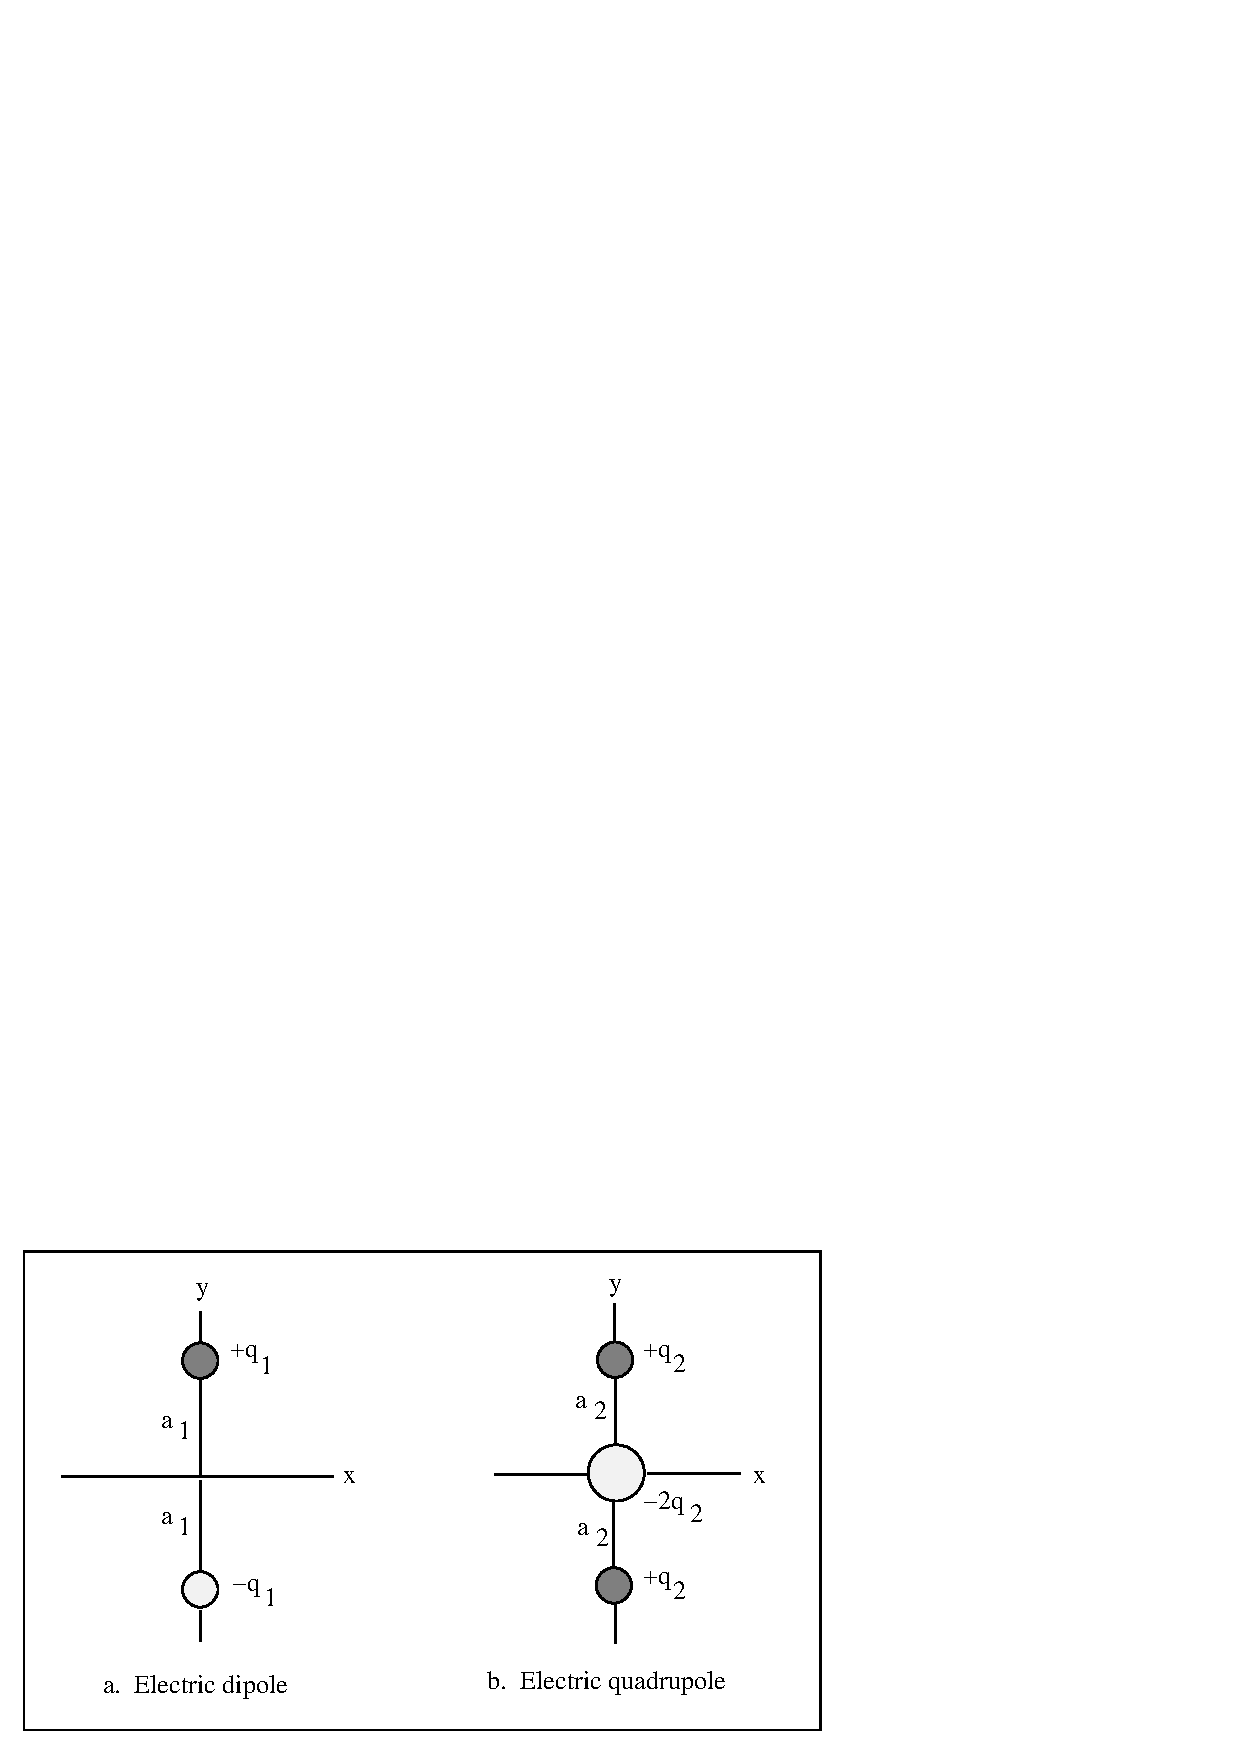
\includegraphics{charge_dist_water_mol/charge_dist_water_mol_fig_1.pdf} \par}
\vspace{0.3cm}

\textbf{Activity 1: The Electric Dipole }

(a) Calculate the electric potential $V$ for the electric dipole for
a point along the $y$-axis, but at a position $\left| y\right| >
a_1$. Your final expression should depend on the position
$y$, the charge $q_1$, and the most probable location $a_1$ of the
charges.
\answerspace{20mm}

\pagebreak[2]
(b) Generate an expression for the potential energy $U$ of the charge
distribution when another charge $q_{test}$ is placed somewhere
on the $y$-axis with $\left| y\right|  > a_1$.
\answerspace{20mm}

(c) Recall the component of the force on a particle is related to
the potential energy of the particle by $F_y  = - \frac{dU}{dy}$.
Calculate the force on the test charge in terms of the position on
the $y$-axis, the charges, and $a_1$.
\answerspace{20mm}

(d) Make the approximation that the test charge is far from the molecule,
i.e., $\left| y\right|  \gg  a_1$, to generate
a new expression for the force.
\answerspace{20mm}

\textbf{Activity 2: The Electric Quadrupole} 

(a) Calculate the electric potential $V$ for the electric quadrupole
for a point along the $y$-axis, but at a position $\left| y\right|  > a_2$. Your final expression should depend on the position $y$, the charge $q_2$, and the most probable location $a_2$ of the
charges.
\answerspace{20mm}

(b) Generate an expression for the potential energy $U$ of the charge
distribution when another charge, $q_{test}$, is placed somewhere
on the $y$-axis with $\left| y\right|   > a_2$.
\answerspace{20mm}

(c) Calculate the force on the test charge in terms of the position
on the $y$-axis, the charges, and $a_2$.
\answerspace{25mm}

\pagebreak[2]
(d) Make the approximation that the test charge is far from the molecule,
i.e., $\left| y\right|  \gg a_2$, to generate
a new expression for the force.
\answerspace{25mm}

\textbf{Activity 3: Distinguishing Between the Two Different Charge
Distributions} 

(a) Construct a table in the space below with column headings $y$ (in Angstroms),
Dipole Force (arbitrary units), and Quadrupole Force (arbitrary units).
The units of distance known as Angstroms are commonly used in atomic
physics. One Angstrom is equal to $10^{-10}$ m.
\answerspace{25mm}

(b) To calculate the force on the test charge one must know the charges
and their positions for each charge distribution ($q_1$, $q_2$, $a_1$, $a_2$). 
These quantities are unknown to us at
this point. However, we want to compare the behavior of the force
due to each as a possible probe of the molecule's charge distribution.
In the expressions you generated in step (d) of Activities 1 and 2
for $\left| y\right| \gg a_1$ or $\left| y\right| \gg  a_2$ the forces depend on some power of $y$. For
\emph{convenience}, set the constant in front of this power of $y$ to
unity. Calculate the forces for the dipole and quadrupole at distances
between 1.5 Angstroms and 5.0 Angstroms in 0.5 Angstrom steps. Enter
your results in the table.

(c) Make a graph of the force due to the dipole and due to the quadrupole
as a function of $y$. Insert a copy of the graph into your notebook.

(d) In many experiments constants like those in your expressions for
the force on the test charge are unknown or poorly known. Suppose,
however, that you are able to accurately measure the radial dependence
of the force on $q_{test}$ at distances far from the  H$_2$O
molecule. If that is the case use the results from steps (b) and (c)
to propose a technique to distinguish between the two candidates for
the charge distribution of  H$_2$O. Support your proposal with
a mathematical argument. (Hint: Consider a ratio involving the measured
force.)
\answerspace{25mm}

(e) Experiment has found that water behaves as an electric dipole,
with the electric dipole moment $q_1 a_1$ measured
to be $6.2 \times 10^{-30}$ C-m. If the charge $q_1$ that creates the dipole
is the charge associated with the protons and electrons
of the molecule, calculate the separation $a_1$ of the charges.
How does it compare with the size of the  H$_2$O molecule, which is
about 1.0 Angstroms?
\answerspace{15mm}


	\include*{capacitance}

%--------------------------------------------circuits
\part{Electric Circuits}
\
%\setcounter{page}{1}
%\setcounter{equation}{0}
%\setcounter{figure}{0}

\section{An Introduction to Electric Circuits}

\begin{comment}
This lab was originally written by Matt Trawick in around 2008, and finally transcribed to Latex for inclusion in this lab manual in 2015.  The goal is to build students' intuition for how circuits work, which students typically really suck at.  More specifically, students have a lot of misconceptions about circuits:  for example, when they do differentiate between current and voltage,they think of a battery as a source of constant current rather than constant voltage.  Lillian McDermott's PER group at Washington did a lot of research into these misconceptions, and many of the exercises in here are specifically based on their findings.  (For all I know, I may even be asking students some of the exact questions they did; at any rate, their work deserves at least a tip of the hat.)

I've deliberately done the lab without mentioning Ohm's law.  (That comes later!)  Students tend to use Ohm's law to calculate stuff without having any clue what's actually going on.  The goal of this lab is to build physical intuition for concepts without turning to plug-and-chug.

The cutting-and-folding paper thing is something I came up with.  I know it feels a little funny to do paper cutting with college students, BUT THIS REALLY WORKS!  I have seen the light bulbs go off over so many of their heads when I show them this!  Students tend to try to memorize "bulbs in parallel have the same voltage, bulbs in series have the same current," but they do so formulaicly with no real understanding, so they forget.  Note to instructors: REALLY PUSH THIS!  Make them do it, and take it seriously!

Equipment notes: 

The circuits here require that the DC power supply have very low internal resistance, which means that any actual power supply works fine.  Actual batteries generally have too high an internal resistance to work well, so for instance students will see bulbs become slightly dimmer when more bulbs are added in parallel. Also, the bulbs in this lab MUST BE IDENTICAL TO EACH OTHER.  Seriously, they should be individually tested as they're put out on the tables to make sure each bulb in the set of three (plus a spare) draws the same amount of current. 

I believe the circuits here are most easily (and intuitively) constructed using banana cables, which means that the bulbs and sockets should also have banana jacks on them.  (I found I could use bulb sockets with screw terminals, then put spade-connector-to-banana-jack adapters on them.

For the multimeters, have plenty of extra fuses on hand, as some fuses will be blown!

I also recommend two pairs of scissors per group, so that each student does their own cutting and folding.  If they both cut, then they will also both fold, and the physical act of folding seems to build a kind of kinesthetic memory for the concept the lab is trying to get across.
\end{comment}

\makelabheader %(Space for student name, etc., defined in master.tex)

\textbf{Objective}

To understand current, voltage, and series and parallel circuits.  And learn how to use a digital multimeter!

\textbf{Apparatus}

\begin{itemize} \itemsep1pt
\item 2 digital multimeters 
\item DC power supply 
\item three matching light bulbs 
\item various wires and alligator clips
\item scissors
\end{itemize}

\textbf{Introduction:}

In this lab, you will measure both electric currents and potential differences using your digital multimeters (DMMs).  Your instructor will show you how to set up your DMM for each kind of measurement.

To measure the electric current in a circuit, you will need to break the circuit, reconnecting it so that current is forced to flow through the meter, as shown below.  (The ``A'' is the symbol for a current meter, or ammeter.)

\begin{center}
%\includegraphics[height=1.5in]{electric_circuits/how_to_measure_current.eps}
\includegraphics[width=0.8\textwidth]{electric_circuits/how_to_measure_current.eps}
\end{center}
\vspace{-0.1in}

Your DMM can also measure the potential difference, in volts between any two points in the circuit.  For this measurement, keep your circuit intact, and simply touch the two leads of the DMM to the two places in the circuit you want to measure between.

\begin{newboxed}
\textbf{For all parts of this lab, keep your power supplies set to a voltage of 3.0 volts, and use the 10A or 20A range of your DMM for measuring currents.  Otherwise we'll blow out lots of bulbs and fuses.}
\end{newboxed}

\vspace{0.1 in}
\textbf{Activity 1: Current and Voltage Measurements}

%\newpage
(a) The circuit below consists of a power supply, two ammeters, and a single light bulb.  For the following circuit, predict which of the two ammeters will measure the larger current.  (Or will they be the same?)

\begin{wrapfigure}[1]{l}{0.3\textwidth}
    \vspace{-0.4 in}
    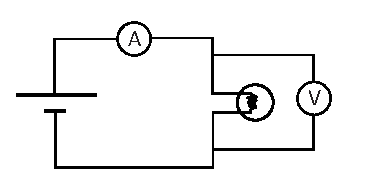
\includegraphics[width=0.3\textwidth]{electric_circuits/circ_diag1.eps}
\end{wrapfigure}

\vspace{0.2 in}
Prediction:
\vspace{1.2 in}

%\newpage
\pagebreak
(b) Build the circuit above, using your two DMMs to measure the current $I$ that flows at the two points in the circuit shown.  Record your measurements.  Was your prediction correct?
\vspace{1 in}

(c) Remove one of your two DMMs from the circuit, and use it to measure some voltage differences in the circuit as shown.  Hold the black lead at point a, and move the red lead to b, c, and d, recording the results.

\begin{wrapfigure}[2]{r}{0.35\textwidth}
    \vspace{-0.5 in}
    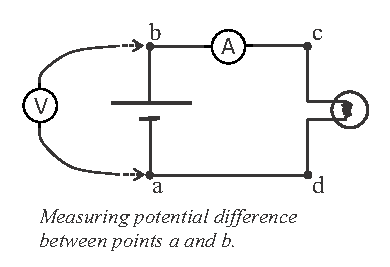
\includegraphics[width=0.35\textwidth]{electric_circuits/circ_diag2.eps}
\end{wrapfigure}

\vspace{0.3 in}
\hspace{0.5 in} $\Delta V_{ab} = $ \par
\hspace{0.5 in} $\Delta V_{ac} = $ \par
\hspace{0.5 in} $\Delta V_{ad} = $ \par
\vspace{0.6 in}

(d)  Predict the voltage difference between the two points c and d in the circuit above.  Test your prediction with a measurement.  Do they agree? \par
\hspace{0.5 in} Prediction:   $\Delta V_{cd} = $ \par
\vspace{0.2 in}
\hspace{0.5 in} Measurement:   $\Delta V_{cd} = $ \par
\vspace{0.3 in}
(e) How big is the voltage difference between the two ends of a typical wire in your circuit?
\vspace{0.6 in}



(f) How big is the voltage difference across your ammeter?  
\vspace{0.6 in}



(g) Is it reasonable to approximate either or both of the voltage differences in (e) and (f) as zero?
\vspace{0.6 in}



\textbf{Activity 2: Two Light Bulbs in Parallel}

(a) The figure below shows a circuit with a second bulb added.  These bulbs are connected ``in parallel.''  In the drawing shown, is the ammeter measuring current through just one of the lightbulbs, or through both of the lightbulbs?
\vspace{-0.1in}
\begin{flushright}
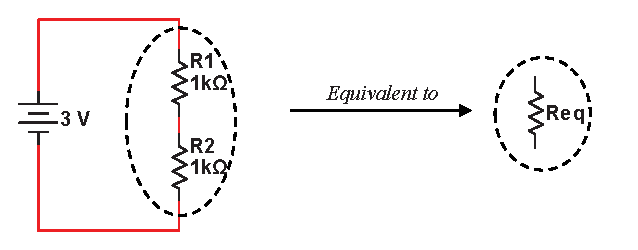
\includegraphics[width=0.4\textwidth]{electric_circuits/circ_diag3.eps}
\end{flushright}
\vspace{-0.1in}


(b) Make a prediction: If you add the second light bulb to your circuit as shown, will the current in the first light bulb increase, decrease, or stay about the same?  Build the circuit and test your prediction. \par
\hspace{0.5 in} Prediction:   \par
\vspace{0.2 in}
\hspace{0.5 in} Measurement:  \par
\vspace{0.3 in}

(c)  In the circuit you have just built, how much current is flowing from the power supply?  Make a prediction, and use a second ammeter to test your prediction. \par
\hspace{0.5 in} Prediction:   \par
\vspace{0.2 in}
\hspace{0.5 in} Measurement:  \par
\vspace{0.3 in}

\begin{center}
\framebox[1.1\width]{\textit{This is a good time to check with your instructor to be sure your measurements are on the right track.}} \par
\end{center}

%\textit{This is a good time to check with your instructor to be sure your measurements are on the right track.} \par

(d) What is the voltage difference across each of the two light bulbs in the circuit above?  Use one of your DMMs as a voltmeter to test your prediction. \par
\hspace{0.5 in} Prediction:   \par
\vspace{0.2 in}
\hspace{0.5 in} Measurement:  \par
\vspace{0.3 in}

(e) Here's a neat way to visualize electric potential, using an analogy with gravitational potential energy.  For the simple circuit that you made in activity one, imagine the circuit drawn on a piece of paper shaped like a loop, with the paper folded so that height above the table corresponds to electric potential as shown below.
\begin{center}
\includegraphics[width=0.5\textwidth]{electric_circuits/how_to_fold.eps}
\end{center}
\vspace{-0.1in}

On the last pages of this lab are some big circuit diagrams for you to cut out.  First, find the diagram of the circuit with two light bulbs, and use scissors to cut it into a shape with two loops.  Then fold your paper so that the height above the table corresponds to changes in potential energy.  Discuss your figure with your instructor.  Yes, you REALLY have to do this! 
\vspace{0.2 in}

(f) Is your power supply acting more like a source of fixed current, or a source of fixed voltage?  (What changes and what stays the same when you connect one or two bulbs to your power supply?) Explain.
\vspace{0.6 in}

\textbf{Activity 3: Two Light Bulbs in Series} \par
\nopagebreak
(a) The circuit below shows two light bulbs connected to the power supply in series.  Make predictions for the current in each of the bulbs, and the voltage difference across each bulb.  Then build the circuit and test your predictions with measurements.  \par

\begin{wrapfigure}[1]{r}{0.3\textwidth}
    \vspace{-1.1 in}
    \includegraphics[width=0.3\textwidth]{electric_circuits/circ_diag4.eps}
\end{wrapfigure}

\vspace{0.1 in}
\renewcommand{\arraystretch}{1.6}
\hspace*{0.5in}
\begin{tabular}{l l}
Predictions: \hspace{0.5in} & Measurements: \\
$I_1 =$ & $I_1 =$ \\
$\Delta V_1 =$ & $\Delta V_1 =$ \\
$I_2 =$ & $I_2 =$ \\
$\Delta V_2 =$ & $\Delta V_2 =$ \\
\end{tabular}
\renewcommand{\arraystretch}{1.0}
\vspace{0.3in}

(b)  Cut out the picture of this circuit from the final pages of your lab, and fold it so that height above the table represents electric potential.  Discuss your figure with your instructor. 

\textit{(A quick note for those who have studied circuits before:  You may have expected the current in each of the bulbs to be exactly half of the current through a bulb in the previous exercises.  That would be true if the bulbs were regular resistors.  But in fact, the ``resistance'' of these bulbs changes as they get hot, so they don't obey Ohm's law.)}

\textbf{Activity 4: Bulbs in series and in parallel} \par
\nopagebreak
(a) The circuit shown below includes light bulbs in series and in parallel with each other.  Predict the values of the currents and voltage differences for each bulb, and then test your predictions.  Which bulb or bulbs will be brightest? \par

\begin{wrapfigure}[1]{r}{0.4\textwidth}
    \vspace{-1.0 in}
    \includegraphics[width=0.4\textwidth]{electric_circuits/circ_diag5.eps}
\end{wrapfigure}

\vspace{0.1 in}
\renewcommand{\arraystretch}{1.6}
\hspace*{0.5in}
\begin{tabular}{l l}
Predictions: \hspace{0.7in} & Measurements: \\
$I_1 =$ & $I_1 =$ \\
$I_2 =$ & $I_2 =$ \\
$\Delta V_{ab} =$ & $\Delta V_{ab} =$ \\
$\Delta V_{bc} =$ & $\Delta V_{bc} =$ \\
$\Delta V_{de} =$ & $\Delta V_{de} =$ \\
Brightest bulb: & Brightest bulb: \\
\end{tabular}
\renewcommand{\arraystretch}{1.0}
\vspace{0.3in}

(b) What is the relationship between bulb brightness and current through the bulb?
\vspace{0.5 in}

(c) What is the relationship between bulb brightness and voltage difference across the bulb?
\vspace{0.5 in}

\newpage
\begin{samepage} %This samepage command had no effect whatsoever.  How do I make this behave, without hardcoding a page break?
(d) If we define the electric potential at the negative terminal of the power supply to be at $V=0$ Volts, what is the potential at each of the points a, b, c, d, and e in the circuit drawing above?  
\vspace*{0.6 in}
\end{samepage}

\textbf{Homework}

Problem 1: Consider the following circuit:

\begin{center}
\includegraphics[width=0.45\textwidth]{electric_circuits/circ_diag6.eps}
\end{center}
\vspace{-0.1in}

(a) If we define the electric potential at the negative terminal of the power supply to be at $V=0$ Volts, what is the potential at each of the points a, b, c, d, e, f, and g?  
\vspace{0.7 in}

(b) Rank from smallest to largest the current at each of the lettered points in the circuit.   (You can write ``$I_c<I_a=I_f<I_e…$'' or something like that.) 
\vspace{0.7 in}

(c) Which bulb or bulbs will be brightest?  Which bulb or bulbs will be least bright?
\vspace{1.7 in}

\textit{(Problem 2 is on the next page.  Keep going....)}
\newpage
Problem 2: Consider the following circuit:

\begin{center}
\includegraphics[width=0.5\textwidth]{electric_circuits/circ_diag7.eps}
\end{center}
\vspace{-0.1in}

(a) Which is greater, $\Delta V_{ab}$ or  $\Delta V_{ef}$?  Why?
\vspace{0.6 in}

(b) Which bulb is brighter, the one between a and b, or the one between e and f?  Why?
\vspace{0.6 in}

(c) Which is greater, $I_a$ or $I_e$?  Why?
\vspace{0.6 in}

(d) Which is greater, $I_c$ or $I_b$? Why?
\vspace{0.6 in}

(e) Which is greater, $\Delta V_{ab}$ or  $\Delta V_{cd}$? Why?
\vspace{0.6 in}

(f) Cut out the circuit on the last page of this lab, and fold it so that height above the table represents electric potential.  Now that you have folded it, are there any answers above you’d like to change?  Bring your folded paper to class, and be prepared to discuss your figure with your instructor.
\vspace{0.6 in}

\cleardoublepage %force this cutout page to be on the right hand side.
\begin{center}
\includegraphics[width=0.95\textwidth]{electric_circuits/cutout_page1.eps}
\end{center}

\newpage
[This page left intentionally blank, at least mostly.]
\newpage

\begin{center}
\includegraphics[width=0.95\textwidth]{electric_circuits/cutout_page2.eps}
\cleardoublepage

\end{center}



%\setcounter{page}{1}
%\setcounter{equation}{0}
%\setcounter{figure}{0}

\section{Ohm's Law and Equivalent Resistance}

\begin{comment}
This lab was originally written by Matt Trawick in around 2008, and finally transcribed to Latex for inclusion in this lab manual in 2015.  This lab builds on "Introduction to Electric Circuits" and uses a lot of the same pedagogical approaches.  

Equipment notes: 

I believe the circuits here are most easily (and intuitively) constructed using banana cables, which means that the bulbs and sockets should also have banana jacks on them.  I found I could use bulb sockets with screw terminals, then put spade-connector-to-banana-jack adapters on them. For the resistors, screw each one into a double banana plug (three total).  Avoid alligator clips; students tend to short them together.

For the multimeters, have plenty of extra fuses on hand, as some fuses will be blown!

I also recommend two pairs of scissors per group, so that each student does their own cutting and folding.  If they both cut, then they will also both fold, and the physical act of folding seems to build a kind of kinesthetic memory for the concept the lab is trying to get across.
\end{comment}

Name \rule{2.0in}{0.1pt}\hfill{}Section \rule{1.0in}{0.1pt}\hfill{}Date
\rule{1.0in}{0.1pt}

\textbf{Apparatus}
\begin{itemize}
\item digital multimeters (2)
\item DC power supply 
\item one light bulb
\item 1 k $\Omega$ resistors (2)
\item 2.2 k$\Omega$ resistors (1)
\item various wires
\item scissors (2)
\end{itemize}

\textbf{Introduction:}

In this lab, you will measure both electric currents and potential differences using your digital multimeters (DMMs).  Your instructor will show you how to set up your DMM for each kind of measurement.

\begin{newboxed}
\textit{For all parts of this lab, keep your power supplies set to a voltage of 3.0 volts.  Otherwise we'll blow out lots of bulbs and fuses.}
\end{newboxed}

\vspace{0.1 in}
\textbf{Activity 1: Relationship Between Current and Voltage}

(a) \textit{For the current measurements in this part, be sure your DMM is using the 10 Amp or 20 Amp range.} Connect a single light bulb to your power supply as shown below, measureing both the current $I$ through it and the voltage $\Delta V$ across it as you vary the voltage of the power supply from 0 to 3.0 volts.  Make a graph of $I$ \textit{vs.} $\Delta V$, for voltages of 0.0, 0.1, 0.3, 1.0, and 3.0 volts.  Use graphing software (like Excel) for your graph, and then make a pencil sketch of it in the space below.  Is the relationship between $I$ and $\Delta V$ linear?

\hspace{0.5in}\includegraphics[width=0.3\textwidth]{electric_circuits2/circ_diag1.eps}
\vspace{0.5 in}

(b) \textit{For the current measurements in this part, change your DMM to a range between 40 mA and 400 mA.} Repeat the measurements in part (a), replacing the light bulb with a resistor with bands colored brown, black, red, and gold.  Again, make a graph of $I$ \textit{vs.} $\Delta V$.  Is the relationship between the two linear?
\vspace{1.6 in}

\newpage
(c) Ohm's law says that for some circuit elements, the current through them is proportional to the voltage across them.  The ratio between the two is the resistance, $R=\Delta V / I$ .  (The unit of resistance is an Ohm ($\Omega$), where 1 Ohm = 1 Volt / 1 Amp.)  Which one of the two things you measured in (a) and (b) follows Ohm's law, and what is its resistance?
\vspace{0.7 in}

(d) Your DMM allows you to measure resistance directly, without using your power supply.  Disconnect the resistor from your circuit \textit{completely,} and use your DMM to measure its resistance.  (The leads go in the same holes you used to measure voltage, and the function selector should be turned to ``$\Omega$''.)  What is its resistance?
\vspace{0.5 in}

(e) The light bulb is designed to glow white hot when current flows in it, and the resistance of the tungsten filament depends strongly on temperature.  That's why the bulb doesn’t follow Ohm's law.  From your measurements in (a) does the filament's resistance increase or decrease with temperature?
\vspace{0.6 in}

\textbf{Activity 2: Two Equal Resistors in Series} \par
\nopagebreak
(a) Build the circuit shown below, which has two 1 k$\Omega$ resistors connected in series.  If your power supply is set to 3 volts, what will be the voltage drop $\Delta V$ across each resistor?  Make a prediction, and test your prediction with a measurement.

\begin{minipage}{0.4\textwidth} 
\hspace{0.5in}\includegraphics[width=0.5\textwidth]{electric_circuits2/circ_diag2.eps}
\end{minipage}
\begin{minipage}{0.6\textwidth} 
\vspace{0.2 in}
Prediction: \hspace{0.4 in} $\Delta V_{R1} =$ \hspace{0.8 in} $\Delta V_{R2}=$
\vspace{0.2 in}

Measurement: \hspace{0.2 in} $\Delta V_{R1} =$ \hspace{0.8 in} $\Delta V_{R2}=$ 
\vspace{0.2 in}
\end{minipage}

(b) You saw in Activity 1 that the voltage difference across a resistor is proportional to its current, $\Delta V=IR$.  Make a prediction for the current through the resistors in the circuit.  Test your prediction by inserting a current meter into your circuit and measuring it.  

\vspace{0.2 in}
\hspace{0.4 in} Prediction: \hspace{0.4 in} $I =$ 
\vspace{0.2 in}

\hspace{0.4 in} Measurement: \hspace{0.2 in} $I=$ 
\vspace{0.2 in}

\pagebreak
(c) We can think of the two resistors in series as being equivalent to a single resistor $R_{EQ}$.  What value single resistor $R_{EQ}$ would we have to replace the two 1k$\Omega$ resistors with in order to draw the same current (about 1.5 mA) from the power supply? \par
\nopagebreak
\begin{center}
\includegraphics[width=0.6\textwidth]{electric_circuits2/circ_diag3.eps}
\vspace{0.2 in}
\end{center}

\textbf{Activity 3: Two Different Resistors in Series} \par
\nopagebreak
(a) The circuit below shows a 1 k$\Omega$ and 2.2 k$\Omega$ resistor connected in series.  Which resistor carries the larger current? (Or are they the same?)  Check yourself with a measurement.   The 2.2 k$\Omega$ resistor has bands colored red, red, red, gold.

\begin{minipage}{0.4\textwidth} 
\hspace{0.5in}\includegraphics[width=0.6\textwidth]{electric_circuits2/circ_diag4.eps}
\end{minipage}
\begin{minipage}{0.6\textwidth} 
\vspace{0.2 in}
Prediction: 
\vspace{0.4 in}

Measurement: \ 
\vspace{0.2 in}
\end{minipage}


(b)Which resistor in the circuit above has a larger voltage drop $\Delta V$ across it?   Why?  Check yourself with a measurement.  

\vspace{0.2 in}
\hspace{0.4 in} Prediction:
\vspace{0.2 in}

\hspace{0.4 in} Measurement:  
\vspace{0.2 in}

(c) Imagine replacing the two resistors in series with a single equivalent resistor $R_{EQ}$.  We can write $R_{EQ}$ in terms of the voltage drops across the resistors as

\begin{displaymath}
R_{EQ} = \frac{\Delta V_{EQ}}{I}= \frac{\Delta V_1 +\Delta V_2 }{I}=\frac{\Delta V_1}{I} + \frac{\Delta V_2}{I}
\end{displaymath}

Use the equation above as a start to write an expression for $R_{EQ}$ in terms of $R_1$ and $R_2$ for two resistors in series.
\begin{displaymath}
\textrm{For resistors in series: } R_{EQ} = 
\end{displaymath}

\textbf{Activity 4: Two Resistors in Parallel} \par
\nopagebreak
(a)  The circuit drawn below shows two resistors in parallel.  Which is bigger, $\Delta V_1$ or $\Delta V_2$? (Or are they the same?)

\hspace{0.5 in}\includegraphics[width=0.4\textwidth]{electric_circuits2/circ_diag5.eps}
\vspace{0.2 in}

\pagebreak
(b) Which resistor in the circuit above has a larger current through it?   Why? 
 
\vspace{0.2 in}
\hspace{0.4 in} Prediction:
\vspace{0.2 in}

\hspace{0.4 in} Measurement:  
\vspace{0.2 in}

(c) What are the currents $I_1$ and $I_2$ through the resistors, in terms of $R_1$, $R_2$, and  $\Delta V$? 
\vspace{0.6in}

(d) Imagine replacing the two resistors in parallel with a single equivalent resistor $R_{EQ}$.   We can write the current through the equivalent resistor as $I_{EQ}=I_1+I_2$.  Using the definition $R_{EQ}=  \Delta V ⁄ I_{EQ}$, write an expression for $R_{EQ}$ in terms of $R_1$ and $R_2$, for two resistors in parallel.  (It's not the same as for resistors in series!)

\begin{center}
\includegraphics[width=0.7\textwidth]{electric_circuits2/parallel_equiv.eps}
\vspace{1 in}
\end{center}

\begin{displaymath}
\textrm{For resistors in parallel: } R_{EQ} = 
\end{displaymath}

\textbf{Activity 5: Using Equivalent Resistances to Solve Problems:}

\begin{wrapfigure}[8]{r}{0.3\textwidth}
    \vspace{-0.4 in}
    \includegraphics[width=0.3\textwidth]{electric_circuits2/circ_diag6.eps}
\end{wrapfigure}

%\vspace{0.3 in}
(a) The last page of this lab is a large picture of this circuit.  Cut it out and fold it so that height above the table at each point of the circuit corresponds to electric potential.  

(b) Which two resistors have the same $\Delta V$?  Which two resistors carry the same current $I$?
\vspace {0.6 in}

(c) Next, we're going to use the idea of equivalent resistances to find the current that flows in each of the resistors in the circuit.  The flow chart on the following page will guide you through it.

\begin{center}
\includegraphics[width=0.9\textwidth]{electric_circuits2/step_by_step_circuit.eps}
\end{center}
\textbf{Homework Questions} \par
\nopagebreak
(a) If two resistors are connected in series, do they always carry the same current through them? If not, which one will have the larger current?
\vspace {0.7 in}

(b) If two resistors are connected in series, do they always have the same voltage difference across them?  If not, which one will have the larger voltage difference across it?
\vspace {0.7 in}

(c) If two resistors are connected in parallel, do they always carry the same current through them? If not, which one will have the larger current?
\vspace {0.7 in}

(d) If two resistors are connected in parallel, do they always have the same voltage difference across them?  If not, which one will have the larger voltage difference across it?
\vspace {0.7 in}


	
\section{Ohm's Law}

Name \rule{2.0in}{0.1pt}\hfill{}Section \rule{1.0in}{0.1pt}\hfill{}Date
\rule{1.0in}{0.1pt}

\textbf{Objectives}

\begin{itemize}
\item To investigate the most important principle in electronics.
\item To determine how resistors in series and parallel add.
\end{itemize}
\textbf{Introduction}

The rate at which electric charge flows through a conductor is called
the electric current. In order to have a current, a potential difference,
or voltage is necessary. We first want to determine the relationship
between the potential difference at two ends of a conductor and the
current flowing through it.

\textbf{Note}: Do not turn on a power supply until you are sure your
circuit is correct. If you are at all unsure, please ask your instructor
to approve your setup. Ammeters can be instantly and permanently ruined
by an improper connection. Be sure to turn off the power supply before
making any changes to the circuit.

\textbf{Apparatus}

\begin{itemize}
\item power supply
\item 2 rheostats
\item ammeter
\item voltmeter
\end{itemize}
\textbf{Activity 1: Ohm's Law}

\begin{itemize}
\item Connect two rheostats (or variable resistors) in series as shown in
the figure below. Set R\( _{1} \) at about the halfway point and
R\( _{2} \) at the maximum. Connect an ammeter as shown. Also, connect
a voltmeter across (that is, connect a probe to each side of) R\( _{1} \).
\end{itemize}
\vspace{0.3cm}
{\centering \resizebox*{0.35\textwidth}{!}{\includegraphics{ohms_law_fig_1.eps}} \par}
\vspace{0.3cm}

\begin{itemize}
\item When sure of your circuit, turn on the power supply, and turn
the voltage up all the way..
\item Record the current through the circuit and the voltage across R\( _{1} \).\vspace{10mm}

\item Reduce the resistance of R\( _{2} \) and record the current and voltage
three more times by turning down the rheostat in approximately equal
steps so that for the last time R\( _{2} \) is turned completely down.\vspace{30mm}

\item Turn off the power supply.
\item Plot your four pairs of readings with the voltage on the vertical axis
and the current on the horizontal axis.
\item Fit a straight line to the points, using the origin as a fifth point.
\item Is a straight line a good fit to the data? What does that say about
the relationship between voltage and current?\vspace{15mm}

\item What are the value and meaning of the slope of this line? Write the
equation of the line.\vspace{15mm}

\item Remove R\( _{1} \) from the rest of the circuit and use the ohmmeter
option on the multimeter to measure the resistance of R\( _{1} \).
Does it agree with the slope you found? What is the percent difference?
Replace R\( _{1} \).\vspace{30mm}

\item What is the general relationship between voltage, current, and resistance?
This is Ohm's Law.\vspace{15mm}

\item Why is the origin a legitimate point on the curve?\vspace{15mm}

\end{itemize}
\textbf{Activity 2: Resistors in Series}

\begin{itemize}
\item Turn rheostat R\( _{2} \) to its maximum setting. Connect the multimeter
across this resistor, being sure to set it for reading voltages.
\item When you are sure the circuit is set, turn on the power supply and
record the current and voltage. Turn off the power supply.\vspace{10mm}

\item \textbf{Prediction}: Based on your measurements, predict the resistance
of R\( _{2} \).\vspace{15mm}

\item Remove and measure the resistance of R\( _{2} \). Record the percent
difference between your prediction and measurement. Replace R\( _{2} \).\vspace{30mm}

\item Was the current this time different from the first reading in Activity
1?\vspace{15mm}

\item What can you conclude about the current through two resistors in series?\vspace{15mm}

\item Connect the multimeter across both resistors, being sure to switch
to voltage readout.
\item When you are sure the circuit is correct, turn on the power supply
and record the current and voltage. Turn off the power supply.\vspace{10mm}

\item Has the current changed?\vspace{15mm}

\item Has your previous conclusion been substantiated or refuted?\vspace{15mm}

\item How is the voltage just measured related to the first voltage measurements
in Activities 1 and 2?\vspace{15mm}

\item What can you conclude about the voltage across resistors in series?\vspace{15mm}

\item Using your conclusions concerning voltages across and current through
resistors in series and your formulation of Ohm's law, what can you
conclude about the total resistance in a circuit having two resistors
in series?\vspace{15mm}

\end{itemize}
\textbf{Activity 3: Resistors in Parallel}

\begin{itemize}
\item Connect the two rheostats in parallel as shown in the figure below,
with the ammeter at the point marked A and the voltmeter across the
two rheostats. Set the rheostats at about their halfway settings.
\end{itemize}
\vspace{0.3cm}
{\centering \resizebox*{0.35\textwidth}{!}{\includegraphics{ohms_law_fig_2.eps}} \par}
\vspace{0.3cm}

\begin{itemize}
\item When you are sure the circuit is set up correctly, turn on the power
supply and record the total current through the circuit and the voltage
drop across the parallel resistance combination. Turn off the power
supply.\vspace{10mm}

\item Connect the ammeter to the point marked A\( _{1} \) without disturbing
the rest of the circuit; apply power and record the current through
R\( _{1} \) and the voltage reading. Turn off the power supply.\vspace{10mm}

\item Repeat the above measurements for R\( _{2} \), connecting the ammeter
at A\( _{2} \) instead of A\( _{1} \).\vspace{10mm}

\item Using Ohm's Law, calculate the two resistances of the parallel connection
and also the total resistance of the circuit. Check with the ohmmeter
and determine the percent differences.\vspace{30mm}

\item What is the relationship between the total current and the current
in each of the branches of the parallel circuit?\vspace{15mm}

\item What is the relationship between the total resistance of the parallel
circuit and the resistance of each of the branches (you may want to
look up in a reference what the correct relationship should be and
see if your result agrees with it)?\vspace{15mm}

\item Determine, using Ohm's law, what the voltage was in each branch of
the parallel circuit. Did it make any difference that you didn't reposition
the voltmeter during this activity? On the basis of Ohm's law, does
the result make sense?\vspace{30mm}

\item Can the total resistance of a series combination ever be less than
the resistance of the largest resistor? Explain.\vspace{30mm}

\item Can the total resistance of a parallel combination ever be greater
than the resistance of the smallest resistor? Explain.\vspace{30mm}
\end{itemize}


	\section{Kirchhoff's Rules}

\makelabheader %(Space for student name, etc., defined in master.tex)

\bigskip
\textbf{Introduction}

Two statements comprise Kirchhoff's rules. The first, the so-called
junction rule, restates the conservation of charge; the second, the
so-called loop rule, restates the conservation of energy:

\begin{enumerate}
\item The sum of the currents entering any junction (or node) must equal
the sum of the currents leaving that junction.
\item The algebraic sum of electrical potential changes across all the elements
around any closed loop must be zero.
\end{enumerate}
\textbf{Note}: Do not turn on a power supply until you are sure your
circuit is correct. Please ask your instructor to approve your setup.
Ammeters can have their fuses blown by an improper connection, which is a nuisance to replace.
Be sure to turn off the power supply before making any changes to
the circuit.

\bigskip
\textbf{Apparatus}

\begin{itemize}[nosep]
\item digital multimeters (2)
\item DC power supply
\item 1~k$\Omega$ resistors (2)
\item 2.2~k$\Omega$ resistor
\item various wires and aligator clips
\item masking tape
\end{itemize}

\bigskip
\textbf{Activity}

Build the circuit shown below, with $R_C = 1$~k$\Omega$, $R_A = 1$~k$\Omega$, and $R_B = 2.2$~k$\Omega$. Make sure the power supply is off. Use masking tape to label the resistors in your circuit. As a visual aid, you can also tape down the connecting wires to the table top to make your circuit layout resemble the circuit diagram.

\vspace{0.3cm}
{\centering \resizebox*{0.5\textwidth}{!}{\includegraphics{kirchhoffs_rules/kirchhoffs_rules_fig_1.eps}} \par}
\vspace{0.3cm}

\begin{enumerate}[labparts]

\item Set one of your multimeters to resistance measuring mode. Remove $R_A$ from the circuit and measure its resistance with the multimeter and record the value below. Reconnect $R_A$ back to the circuit. Repeat this for $R_B$ and then for $R_C$.

\hspace{0.5in}$R_A=$

\hspace{0.5in}$R_B=$

\hspace{0.5in}$R_C=$


\item Referring to the circuit diagram above, choose a junction and write an equation
which satisfies Kirchhoff's first rule.
\answerspace{20mm}

\item Identify two closed loops on the circuit which contain at least one
element not included in the other. Write an equation for each loop
that satisfies Kirchhoff's second rule.
\answerspace{30mm}

\item You now have three equations that can be solved for the three currents $I_A$, $I_B$, and $I_C$.
Before doing the algebra, substitute the values of the three resistors that you determined in part~(a) into the loop equations. Further, substitute a value of 3.00~V for the emf. Carry out the algebra to obtain the values of the three currents.
\answerspace{5in}

\item Now use Ohm's law and the rules for combining resistors in series and parallel (i.e. reducing the circuit to equivalent circuits) to calculate the values of the three currents. Again use a value of 3.00~V for the emf and also use the values of the three resistors from your measurements.
\answerspace{3.5in}

\item Are the results of parts (d) and (e) the same? They should be.
\answerspace{15mm}

\item Make sure your circuit is complete and the power supply is still off. Connect one of your multimeters in parallel with the power supply in order to measure the voltage across the terminals of the power supply. Then, connect your second multimeter as an ammeter in series with $R_C$ in order to measure the current $I_C$. Now, turn the power supply on and adjust its output to read 3.00~V on the first multimeter. Record the value of $I_C$ below. Next, repeat the same procedure to measure similarly the currents $I_A$ and $I_B$. (Make sure the first multimeter still reads 3.00~V.) Record the values of the currents below.

\hspace{0.5in}$I_C =$

\hspace{0.5in}$I_A =$

\hspace{0.5in}$I_B =$

\bigskip
\item Do your results agree with those obtained in parts (d) and (e)? How large, in terms of percentage, are the discrepancies? Speculate on what might cause any differences. 

\answerspace{15mm}
\end{enumerate}


\section{Power Dissipation in Resistors}

\instructornote{%
By Matt Trawick, 2015.  Time: $\sim$50 minutes

This is admitedly not the most sophisticated investigation we do, but several students have said this was their favorite lab all semester.

This lab assumes that students have already seen $P=IV$.  But for most students, just being introduced to it doesn't really teach them what power MEANS, in the very visceral sense of things becoming hot to the touch.

The write-up is deliberately somewhat minimalist.  You may need to tell students the ``Rated Power'' for the various resistors, as well as what that means (if you choose).  This lab also doesn't really explain what ``temperature coefficient'' means.   Students also may need some help using the resistor color code.

\textbf{Equipment notes: }

For the resistors, use 100 ohm resistors.  I've typically used:
\begin{itemize}[nosep]
\item 1/8 watt (Currently we have metal film resistors with a weakly positive temperature coefficient.)
\item 1/4 watt (I haven't used this lately.  Three resistors is really enough.)
\item 2 watt (Currently we have 2~W carbon-glass resistors with a strong negative temperature coefficient)
\item 25 watt (These are designed for high power, and should have a positive temperature coefficient, but one that's probably too small to measure.)  Incidentally, I think the 25~W rating is technically only for when its bolted to a heat sink, but they seem to do fine here.
\end{itemize}

The very smallest resistors can actually catch on fire, sometimes with a tiny burst of flame (smaller than a match) so be prepared.  The 2 W resistors will smoke and turn brown.  The biggest power resistors are totally unharmed.  
\textbf{By the way, it's always \textit{much} more memorable for the students if you don't tell them about the catching-on-fire part beforehand.  :-)}

For the multimeters, have some extra fuses on hand, as some fuses may be blown.  However, we can minimize this by presetting the current limiter knobs to just over 300 mA. (Setting the coarse adjustment knob fully counter-clockwise and the fine adjustment knob fully clockwise limits the supply to about what we need.)  Since we're using 100~$\Omega$ resistors, all currents should be safely below the 500~mA rating of the DMM fuses, so even without the current limit, we shouldn't blow any fuses unless students short their wires together.  Which some will.
}

\makelabheader %(Space for student name, etc., defined in master.tex)

\bigskip
\textbf{Apparatus}
\begin{itemize} [nosep]
\item digital multimeters (2)
\item DC power supply 
\item various resistors
\item banana cables and aligator clips
\end{itemize}

\textbf{Activity 1: Measuring Resistances}

(a) You have at your lab station several different resistors: some small ones with colored bands around them, and one much larger one encased in bronze-colored metal.  Write a brief description of each resistor along with their ``nominal'' resistances (that is, the values they're supposed to have) in the table below.  Some resistors have their nominal resistance $R$ printed directly on them.  For the smaller resistors with colored bands, you can find thier nominal resistance using the resistor color code as described in Appendix \ref{resistor_code}.  

\begin{center}
{\renewcommand{\arraystretch}{2.0}
\begin{tabular}{|C{3.8in}|c|c|c|} \hline 
Physical description, size, and colors of bands (if applicable) & Nominal $R$ & Measured $R$ & Rated Power \\ 
\hhline{|=|=|=|=|}
& & & \\ \hline 
& & & \\ \hline 
& & & \\ \hline 
& & & \\ \hline 
\end{tabular} }
\end{center}

(b) Measure the actual resistance of each resistor using your digital multimeter (DMM), and record your values in the table above.  To measure resistance, set the DMM to ``$\Omega$'' and put the two leads in the jacks labeled ``COM'' and ``V-$\Omega$''.  Are your measurements consistent with the nominal value of each resistor, to within their stated tolerances?
\answerspace{0.6in}

(c) What is the relationship between the physical size of the resistors and their resistance?
\answerspace{0.8in}

\begin{wrapfigure}[6]{r}{0.2\textwidth}
    \vspace{-0.5 in}
    \includegraphics{electric_power/resistor_sizes.eps}
\end{wrapfigure}

(d) Write the ``rated power'' of each resistor in your table.  This is the maximum power a resistor can dissipate while still maintaining its characteristics.  Large resistors often have their rated power printed directly on them.  For the smaller ones, you would need to look at the label on the box they came in to know for sure, but you can generally estimate the rated power from the size of the resistor, based on the life-sized drawing to the right. 


\pagebreak
\textbf{Activity 2: Measuring Voltage, Current, and Power}

\begin{wrapfigure}[8]{r}{0.3\textwidth}
    \vspace{-0.4 in}
    \includegraphics[width=0.3\textwidth]{electric_power/circ_diagram_bw.eps}
\end{wrapfigure}

(a) Connect the physically largest resistor to the power supply as shown in the circuit diagram to the right, using two multimeters to precisely measure both the current $I$ and the voltage drop $\Delta V$ across the resistor.  As you increase the voltage across the resistor, calculate both the power $P$ dissipated in it, and its resistance as calculated by $\Delta V/I$.  At each value, feel the resistor (\textit{carefully, so you don't burn your fingers!}) to see if it is getting hot.  To get accurate current readings, use the smallest current range you can.

\vspace{0.2in}

%\begin{center}
%\includegraphics[width=1.0\textwidth]{electric_power/iv_table.eps}
%\end{center}

\newcommand{\maketableforivmeasurements}{
\begin{center}
{\renewcommand{\arraystretch}{2.0}
\begin{tabular}{|l|c|C{0.6in}|C{0.6in}|c|C{2.0in}|} \hline 
\multicolumn{6}{|l|}{Resistor (physical size, appearance, and value):} \\
\hline
$\Delta V$ (nominal) & $\Delta V$ (measured) & $I$ & $P$ & $\Delta V / I$ ($\Omega$) & How hot?\\ 
\hhline{|=|=|=|=|=|=|}
0.3 volts & & & & & \\ \hline 
1 volt & & & & & \\ \hline 
3 volts & & & & & \\ \hline 
10 volts & & & & & \\ \hline 
30 volts & & & & & \\ \hline 
\end{tabular} }
\end{center}
}
\maketableforivmeasurements

(b)  Based on your measurements, did the resistance increase, decrease, or stay the same as you increased the current?  (Be careful: are your measurements of current and voltage precise enough to support your conclusion?)  Is the temperature coefficient positive or negative for this resistor? 
\answerspace{1.0in}

\begin{center}
\framebox[1.07\width]{\textit{This is a good time to check with your instructor to be sure your measurements are on the right track.}} \par
\end{center}

(c) Now repeat your measurements for each of the other resistors, recording results in the tables below.  \textit{Again, be careful not to burn your fingers!}

\maketableforivmeasurements

\maketableforivmeasurements

\maketableforivmeasurements


(d) Now that they are no longer hot, make a final resistance measurement for each resistor (or whatever is left of it).  Have any of their resistances changed permanently?
\answerspace{1.0in}

(e) Can you determine the sign of the temperature coefficient (positive or negative) for any of your resistors?
\answerspace{1.0in}


(f) What difference did the physical size of the resistor make in the results of any of your measurements?  (Like, for instance, how hot they got and which resistors survived the experiment.)  Why did size make a difference?
\answerspace{1.0in}







\section{Charging and Discharging Capacitors (RC circuits)}

\begin{comment}
This lab was originally written by Matt Trawick in around 2008, and finally transcribed to Latex for inclusion in this lab manual in 2015.  This lab builds on "Introduction to Electric Circuits" and uses a lot of the same pedagogical approaches, but can be used independently.

IMHO, this lab is flat out much better than the existing lab, titled ``RC circuits,'' for lots of reasons:
1. The old lab relies on the internal resistance of analog voltmeters, about 3000 ohms.  This makes it hard for students to see and understand what R actually is, since the meter is a meter first, and a resistor only secondarily.  Using the meter also makes it harder to change R, and the old lab never has students test different resistor values. This new lab uses actual resistors for the job.  (Besides, using analog voltmeters is insanity; nobody outside UR has used them since the Nixon administration.)

2. The old lab uses only one capacitor, so students never see how the time constant depends on C.

3. Pedagogically, the old lab starts with equations, whereas the new lab starts with pictures of circuits and qualitative questions, before working up to an equation for a discharging capacitor at the end of the lab.

4. The new lab explicitly has students make qualitative predictions, and then test them.  The old lab does not.

5.  The old lab talks about the ``half-life'' of an RC circuit.  ``half life'' is used for nuclear decay, but is basically never used for RC circuits in the real world.

In summary, the old ``RC circuits'' lab should be removed, and replaced with this one.

When I teach this lab, I usually wait until students are finished with activity 1 (so they've seen charging and discharging with their own eyes, so to speak) before I launch into a quick refresher lecture about what's happening, and how charge is going through the resistor and building up on one side of the capacitor, but charge is draining away from the other side, and so on.  This is also where I use a water analogy, where the battery is a pump, the resistor is a constriction in the pipe, and the capacitor is a place where the pipe gets wide, and a rubber membrane is stretched across it.

As with any lab, some students finish quickly, some not so much.  I generally cut off the lab when the slowest students have finished part 2(g).  Some students will have figured out on their own that V(t) is a decaying exponential, and some won't have.  I'm okay with that; I'll talk about it in a lecture for those who didn't get there on their own.

Equipment notes: 

I believe the circuits here are most easily (and intuitively) constructed using banana cables, which means that the resistors and capacitors should all be mounted ahead of time into dual banana socckets.  DPST knife switches should also have banana jacks attached to them.  

The values of resistors and capacitors used here are not an accident.  The RC time constants used are slow enough to be easily visible and measurable by the students.  Also, the resistance values are low enough that they are safely below the ~1 Mohm input impedance of the pasco 750 boxes.   That pushes the capacitors to fairly high values, and you can run into troubles there if the capacitors have a high leakage current.  For this reason, it's important to use capacitors with a reasonably low leakage.  
\end{comment}

\makelabheader %(Space for student name, etc., defined in master.tex)

\vspace{0.1in}
\textbf{Apparatus}
\vspace{-\parskip} 
\begin{itemize}[nosep]%[nolistsep]
%\setlength\itemsep{-4pt}
%\setlength\topsep{-6pt}
%\setlength\partopsep{-6pt}
%\vspace{-0.15in}  %There's gotta be a better way to tame this list spacing than this!  --MT
\item Digital multimeters (2) 
\item DC power supply 
\item Pasco 550 interface, with voltage leads
\item Resistors: 10 k$\Omega$ and 27 k$\Omega$
\item Capacitors: 470 $\mu$F and 1000 $\mu$F (``low leakage'')
\item 4 dual banana connectors for resistors and capacitors
\item DPST knife switch with banana jack connectors
\item About six connecting wires
\end{itemize}

\textbf{Activity 1: What's happening?}

Build the circuit shown in the diagram below.  The switch terminal labeled ``2'' in the diagram is the center terminal on your switch.

\begin{minipage}{0.82\textwidth}
\begin{newboxed}
\vspace{-0.2 in}
\textit{Be sure to connect the “negative” end of the capacitor to the negative terminal of the power supply, or it may explode and hurt you.  The negative end of the capacitor is marked with a long stripe down the side of the capacitor with negative signs (``$-$'') on it.  Ask your instructor for help if you are not sure.}
\vspace{-0.1 in}
\end{newboxed}
\end{minipage}
\begin{minipage}{0.17\textwidth}
\includegraphics[width=1.0\textwidth]{rc_circuits/capacitor2_bw.eps}
\end{minipage}

\begin{center}
\vspace{-0.3 in}
%\includegraphics[width=0.6\textwidth]{rc_circuits/circuit_diagram_bw.eps}
\includegraphics[width=0.6\textwidth]{rc_circuits/single_dc_capacitor3.eps}
\vspace{-0.1 in}
\end{center}

(a) When you move the switch to position ``1,'' so that terminals 1 and 2 are connected, what happens to the voltage difference $\Delta V_C$ across the capacitor?
\answerspace{0.6in}

(b)  With the switch in position ``1,'' what is happening to the charge $Q$ stored on the capacitor?
\answerspace{0.6in}

(c)  Now move the switch to position ``3,'' so that terminals 2 and 3 are connected.  What happens to the voltage difference $\Delta V_C$ and the charge $Q$ on the capacitor?
\answerspace{0.7in}

\pagebreak[2]
(d) Starting with $\Delta V_C$ near zero, (say $\Delta V_C \lesssim 1$~V) move the switch to position ``1'' (charging) and observe the current $I$ measured by your DMM.  (You'll need to set your DMM to a low current scale.)  As the capacitor's charge increases, does the current you measure increase, decrease, or remain constant?
\answerspace{0.5in}

(e) Once the capacitor has been charged (say $\Delta V_C \gtrsim 9$~V) move the switch to position ``3'' (discharging).  Is the sign of the current on your meter the same as in part (d), or is it different?  What is the physical meaning of the sign?
\answerspace{0.7in}

\textbf{Activity 2: Drawing graphs}

Because the voltage $\Delta V_C$ is changing, it will be useful to use your computer to graph $\Delta V_C$ \textit{vs.} time.  Put the two red and black leads from the 550 interface box where your digital voltmeter is connected to your circuit.  (You can keep the DMM plugged in too.)

To record voltage versus time data, go to \textit{Start $\longrightarrow$ Programs $\longrightarrow$ PhysicsApplications $\longrightarrow$ Datastudio}. Select the option Create Experiment.  You will see an image of the 550 interface box.  On this image, click on the channel A input.  You will see a list of sensors.  Scroll down to the Voltage Sensor and select by clicking OK.  Finally open a graph display by double clicking on the Graph option (on the left).

(a)  Now take some data.  On the axes below, draw sketches below showing $\Delta V_C$ \textit{vs.} time starting when the switch is moved into position ``1'' (charging) and position ``3'' (discharging).  Include a scale on the vertical axis.

%\vspace{1.5in}
\begin{center}
\vspace{-0.4 in}
\includegraphics[width=0.95\textwidth]{rc_circuits/vc_axes.eps}
\vspace{-0.1 in}
\end{center}

(b) Repeat the experiment above, this time focusing on the current measured by your DMM.  On the axes below, draw sketches below showing $I$ \textit{vs.} time when the capacitor is charging and discharging.  Include a scale on the vertical axis.
\begin{center}
\vspace{-0.3 in}
\includegraphics[width=0.95\textwidth]{rc_circuits/current_axes.eps}
%\includegraphics[width=0.6\textwidth]{rc_circuits/current_axes.eps}
\vspace{-0.1 in}
\end{center}

\begin{wrapfigure}[5]{r}{0.07\textwidth}
    \vspace{-0.2 in}
\includegraphics[width=0.07\textwidth]{rc_circuits/shorted_resistor_bw.eps}
\end{wrapfigure}


(c)  Helpful hint: if you get tired of waiting forever for $\Delta V_C$ to rise and fall, you can briefly ``short out'' the resistor by connecting an additional wire across it, as shown to the right.  
How does ``shorting out'' the resistor affect $\Delta V_C$ when the capacitor is charging?  When the capacitor is discharging?
\answerspace{0.7in}

\pagebreak[2]
\textbf{Activity 3: Measuring the time constant}

(a) Start with the capacitor fully charged at about 10 volts.  Then (with the resistor not shorted out) move the switch to position “3” to discharge the capacitor.  How long does it take for $\Delta V_C$ to drop to 1/3 of its original level (that is, from 10 volts to about 3.3 volts)?
\vspace{0.8in}

(b) If you repeat part (a) with a resistance $R = 10$ k$\Omega$ how do you expect your result to change?  Make a prediction and then test it.

\vspace{0.2 in}
\hspace{0.4 in} Prediction:
\vspace{0.2 in}

\hspace{0.4 in} Measurement:  
\vspace{0.2 in}

%\pagebreak
(c) Go back to using the 27 k$\Omega$ resistor.  Now, if you repeat part (a) with a capacitance of $C=1000$ $\mu$F, how do you expect your result to change?  Make a prediction and then test it.

\vspace{0.2 in}
\hspace{0.4 in} Prediction:
\vspace{0.2 in}

\hspace{0.4 in} Measurement:  
\vspace{0.2 in}

(d) The time it takes for $\Delta V_C$ to fall to about a third of its original value (actually to $1/e$ of its value, where $e=2.71828…$) is called the time constant, $\tau$.   Fill in the following table:

%For fixed width columns:
%These are now defined in master.text, to avoid  warnings when the definition is repeated in each file.
%columntype{L}[1]{>{\raggedright\arraybackslash}p{#1}}
%\newcolumntype{C}[1]{>{\centering\arraybackslash}p{#1}}
%\newcolumntype{R}[1]{>{\raggedleft\arraybackslash}p{#1}}

\vspace{0.1 in}
\renewcommand{\arraystretch}{1.8}
\hspace*{0.5in}
%\begin{tabular}{|c | c| >{\centering}m{1in} |}
\begin{tabular}{|c | c| C{1in} |}
\hline
$R$ & $C$ & $\tau$ \\ \hline
10 k$\Omega$ & 470 $\mu$F &\\ \hline
27 k$\Omega$ & 470 $\mu$F &\\ \hline
10 k$\Omega$ & 1000 $\mu$F &\\ \hline
27 k$\Omega$ & 1000 $\mu$F &\\ \hline
\end{tabular}
\renewcommand{\arraystretch}{1.0}
\vspace{0.2in}

(e) What is the mathematical relationship between $R$, $C$, and $\tau$? Write a single equation that relates the three.
\vspace{0.7in}

(f) Looking at your graphs, what is the functional form of $\Delta V_C$ \textit{vs.} time  for a discharging capacitor?  Try moving your data to Excel and fitting it to test your hypothesis.
\vspace{0.7in}

	\include{rc_circuit}
	\include{lr_circuit/lr_circuit}
	\include*{lrc_circuit/lrc_circuit} %not used in 2015

%--------------------------------------------
\part{Magnetism}
\
	
\section{Magnetism: Qualitative Interactions and Compasses}

\makelabheader %(Space for student name, etc., defined in master.tex)

\textbf{Objectives}

\begin{itemize}
\item To investigate the characteristics of magnets.
\item To understand how a compass works.
\end{itemize}
\textbf{Introduction} 

The electric interaction, you probably know, is not the only one in
which opposites attract and likes repel. Magnetic interactions have
similar characteristics. All simple magnets, regardless of size, are
bipolar: there are two magnetic poles. Consider this question, then:
Can we talk about like and unlike as we do for electricity?

\textbf{Apparatus}

\begin{itemize}
\item 2 bar magnets 
\item 2 cylindrical magnets 
\item rods and clamps
\item wool cloth
\item rubber rod
\item string
\end{itemize}
\textbf{Activity 1: The Characteristics of Magnets}

\begin{enumerate}
\item Feel the attraction between two magnets when pulled apart after having
come together without effort on your part. Describe qualitatively
in terms of strength and separation.\vspace{15mm}

\item Feel the repulsion when one of them is turned around and pushed toward
the other. Describe as in step 1.\vspace{15mm}

\item Note and describe the difference in (strength and direction of) interactions
between the ends and the middle.\vspace{15mm}

\end{enumerate}
\textbf{Activity 2: How a Compass Works}

\begin{enumerate}
\item Identify geographic north and south.
\item Hang one of the cylindrical magnets horizontally from a horizontal rod.
\item When it comes to rest, along which geographical line does the magnet
lie? \vspace{15mm}

\item Which end (colored or uncolored) is the \char`\"{}north-seeking\char`\"{}
end?\vspace{15mm}

\item Remove the cylindrical magnet and repeat step 2 with the second cylindrical magnet. Answer, again, the questions above.\vspace{15mm}

\item What happens when you bring the \char`\"{}north-seeking\char`\"{}
end of the first magnet near the hanging one's north-seeking end?\vspace{15mm}

\item What happens when you bring the first magnet's opposite end near the
second's north-seeking end?\vspace{15mm}

\item What about the first magnet's north-seeking end near the opposite
end of the hanging one?\vspace{15mm}

\item What happens when you bring the opposite ends near one another?\vspace{15mm}

\item Define in your own words like and unlike poles?\vspace{15mm}

\item What always happens between like poles?\vspace{15mm}

\item What always happens between unlike poles?\vspace{15mm}

\item Determine with a labelled bar magnet which end of your hanging magnet
should be identified as the north pole and which the south.
\vspace{10mm}
\item Why do we identify one end of a magnet as the north pole and the other
as the south?\vspace{15mm}

\item In your own words, explain a compass.\vspace{15mm}

\item In terms of magnetism, what is the earth?\vspace{15mm}

\item Charge a rubber rod with the wool cloth and bring it near the ends
of the suspended magnet; describe its effect on the magnet.\vspace{15mm}

\item Does a south magnetic pole repel a negative electric charge?\vspace{15mm}

\item Does a north magnetic pole attract a negative electric charge?\vspace{15mm}
\end{enumerate}


\include{magnetism_2/magnetism_2}
\include{magnetism_3/magnetism_3}
	\setcounter{equation}{0}

\section{Magnetic Field of the Earth}

\makelabheader %(Space for student name, etc., defined in master.tex)

\textbf{Objective}

\begin{itemize}
\item A measurement of the earth's magnetic field.
\end{itemize}
\textbf{Introduction} 

The magnetic field lines of a bar magnet, though emanating from its
full length, are densest near the poles. These lines are typically
not perpendicular to the faces of the magnet. The Earth, as you know,
is like a giant bar magnet, with its magnetic south pole near its
geographic north pole.

The field lines of the Earth's magnetic field, therefore, tend to
point obliquely at any given spot on its surface. The angle (let's
call it \( \phi  \)) that a line makes with a surface is known as
its \emph{dip angle} (see figure). Thus, each locality on earth has
its characteristic value for \( \phi  \) with regard to the terrestrial
magnetic field.

\begin{center} \begin{picture}(200,70) \put(0,0){\line(1,0){200}} \put(150,50){\vector(-2,-1){100}} \put(150,50){\vector(0,-1){50}} \put(150,50){\vector(-1,0){100}} \put(100,60){\makebox(0,0){$B_h$}} \put(160,25){\makebox(0,0){$B_v$}} \put(90,30){\makebox(0,0){$\bf B$}} \put(75,6){\makebox(0,0){$\phi$}} \put(60,0){\oval(10,10)[tr]} \end{picture} \end{center}

The horizontal component of the Earth's magnetic field,

\begin{equation}
B_h = B\cos\phi,
\end{equation}

causes the magnetized needle of a compass to align in the geographic
north-south direction.

%%This is about 1000 times more complicated than it has to be!
% by producing a torque on it. Recall that the
%magnitude of a torque is \( \tau  \) = r F\( \sin \theta  \), where
%F is the force, r is the distance from the axis of rotation to the
%point at which the force acts, and \( \theta  \) is the angle between
%the line from the axis of rotation to the point of interaction and
%the direction of the force.
%
%\begin{center} \begin{picture}(200,75) \put(0,0){\line(0,1){10}} \put(150,0){\line(0,1){10}} \put(65,5){\vector(-1,0){65}} \put(85,5){\vector(1,0){65}} \put(75,5){\makebox(0,0){$\bf r$}} \put(0,15){\circle*{3}} \put(80,55){\makebox(0,0){$\tau = r F \sin\theta$}} \put(150,15){\vector(0,1){50}} \put(150,15){\vector(3,4){37.5}} \put(160,20){\makebox(0,0){$\theta$}} \put(130,35){\makebox(0,0){$F \sin\theta$}} \put(170,50){\makebox(0,0){$\bf F$}} \thicklines \put(0,15){\line(1,0){200}} \end{picture} \end{center}
%
%The force on the compass is due to the Earth's magnetic field,
%F = pB, where p is the so-called \emph{pole strength} (recall that
%F = qE, for static electric fields, where q is the charge). In this
%case, the force acts on both ends of the magnet, so that r (the distance
%from the axis of rotation to the point at which the force acts) is
%half the length of the compass needle, $l$; \( \theta  \) is the
%angle between the alignment of the compass needle and the direction
%of B\( _{h} \). Hence, the torque on a compass needle due to the
%Earth's magnetic field is
%
%\begin{displaymath} \tau_e = plB_h\sin\theta. \end{displaymath}
%

You will use a tangent galvanometer to produce an additional horizontal
magnetic
field perpendicular to the Earth's field (in other words, one that
points east or west).
A tangent galvanometer consists of a vertical, circular coil of wire
with N turns, a pedestal compass at the center of the coil, and electrical
contacts so that a direct current can be established in the coil.
The magnetic field at the center of the galvanometer coil caused by a current
I in the coil is

\begin{equation}
B_c = N\frac{\mu_0I}{2R}
\end{equation}

where R is the radius of the coil and \( \mu _{0} \) is the permeability
of free space (1.25664 x 10\( ^{-6} \) T\( \cdot  \)m/A). B\( _{c} \)
is perpendicular to the vertical plane of the coil. If the plane of
the coil is placed in the north-south direction (that is, parallel
to the compass needle when there is no current in the coil), then,
when there is current in the coil, the compass will be influenced
by two perpendicular fields, B\( _{h} \) and B\( _{c} \). 
The compass needle will now point in the direction of the vector
sum ${\bf B}_h+{\bf B}_c$.  

Let $\theta$ be the angle through which the compass needle turns
when the current in the tangent galvanometer is turned on.
In other words, $\theta$ is the angle between ${\bf B}_h$ and
${\bf B}_h+{\bf B}_c$.  Sketch a picture of these vectors, and
use it to convince yourself that

%The
%latter provides a second torque (see figure, checking carefully the
%angles, \( \cos \theta =\sin (\frac{\pi }{2}-\theta ) \) ):
%
%\begin{displaymath} \tau_c = plB_c\cos\theta \end{displaymath}
%
%\begin{center} \begin{picture}(150,150) \put(10,75){\line(1,0){100}} \put(60,25){\line(0,1){100}} \put(5,75){\makebox(0,0){W}} \put(60,130){\makebox(0,0){N}} \put(115,75){\makebox(0,0){E}} \put(60,20){\makebox(0,0){S}} \put(34,40){\vector(3,4){54}} \put(34,40){\vector(-1,0){10}} \put(34,40){\vector(0,-1){10}} \put(88,112){\vector(1,0){10}} \put(88,112){\vector(0,1){10}} \put(65,90){\makebox(0,0){$\theta$}} \multiput(34,40)(12,-9){4}{\line(4,-3){10}} \multiput(88,112)(12,-9){4}{\line(4,-3){10}} \multiput(60,75)(12,-9){2}{\line(4,-3){10}} \put(15,40){\makebox(0,0){$\scriptstyle pB_c$}} \put(108,112){\makebox(0,0){$\scriptstyle pB_c$}} \put(34,25){\makebox(0,0){$\scriptstyle pB_h$}} \put(88,127){\makebox(0,0){$\scriptstyle pB_h$}} \put(92,81){\makebox(0,0){$\scriptstyle r$}} \put(104.5,43){\makebox(0,0){$\scriptstyle l$}} \put(89,77){\vector(-3,-4){10}} \put(95,85){\vector(3,4){10}} \put(100,37){\vector(-3,-4){20}} \put(109,49){\vector(3,4){20}} \end{picture} \end{center}
%
%When current is established in the coil, the needle will rotate through
%an angle \( \theta  \) with respect to the plane of the coil until
%the opposing torques are equal in magnitude. Thus, when equilibrium
%is established, we have
%
%\begin{displaymath} \tau_e = \tau_c \Rightarrow plB_h\sin\theta = plB_c\cos\theta \end{displaymath}

\begin{equation}
%\begin{displaymath} 
B_h = \frac{B_c}{\tan\theta} 
%\end{displaymath}
\end{equation}

\vskip 1in

By measuring the angle $\theta$, we can determine $B_h$.  
If we then measure the dip angle $\phi$, we can determine
the Earth's magnetic field from equation (1) above.

\textbf{Apparatus}

\begin{itemize}
\item tangent galvanometer 
\item power supply 
\item DC ammeter (0-1 amp)
\item banana plug leads (1 red, 2 black) with alligator clips
%\item switch
\item compass
\item ruler 
\item dip angle compass 
%\item wooden stand
\end{itemize}
\vspace{15mm}
\textbf{Activity}

\begin{enumerate}
\item Measure and record on the accompanying data sheet the diameter D of
the galvanometer coil. Calculate and record the radius R of the coil.
\item Count and record the number of turns, N, of the coil.
\item With the power supply off, connect its positive and negative terminals 
to the tangent galvanometer and  a DC ammeter (in series). 
Be sure the ammeter is connected in \underline{series} with 
the coil. Use long wires to connect the outside terminals of the coil
to the circuit so that the coil may be removed from the magnetic effects
of the ammeter and power supply. Be sure no magnetic material other
than the compass is in the vicinity of the coil. Turn the coarse current 
control on the power supply all the way up and the voltage controls all the 
way down.
\item Place the compass on the platform of the tangent galvanometer and rotate  
the galvanometer until the compass needle is aligned with the plane of the wire 
coil of the galvanometer. Rotate the compass body so that the needle points 
north and south on the compass.
\item Turn on the power supply and slowly turn up the fine voltage control 
until the current is about 0.2 A as measured with the orange ammeter.
Note that the compass needle rotates. It might be a good idea to tap
lightly the face of the compass to be sure the needle hasn't become
stuck. Record the current and the displacement angles at both the
north and south poles of the needle. Calculate B\( _{c} \) from equation (2).
\item Average the north and south angles; use this average to calculate 
B\( _{h} \) from equation (3).
\item Repeat steps 5 and 6 for currents of 0.4 A, 0.6 A, and 0.8 A.
\item Reverse the current (by switching the two leads at the galvanometer coil)
 and repeat steps 5, 6 and 7.
\item Determine and record the dip angle at two separate locations in the 
classroom (using the dip angle compasses). Average these measurements and use 
the result for the dip angle, \( \phi  \).
\item Using equation (1) above, calculate the Earth's magnetic field 
\textbf{B} for each set of data. Remember that in equation (1), \( \phi  \) 
is the \underline{dip angle}, not the displacement angle of the compass.
Calculate an average value for \textbf{B} and a standard deviation.
How far off, in terms of numbers of standard deviations, is your result
from the accepted value for Richmond, $5.1 \times 10^{-5}$ T?
\end{enumerate}
\hrulefill

\newpage

{\centering \textbf{Data Sheet}\par}

%Diameter of Coil, D (m) \> \rule{2cm}{.1pt}  

Diameter of Coil, D (m)  \rule{2cm}{.1pt}  

Radius of Coil, R (m) \rule{2cm}{.1pt} 

Number of Turns of Coil, N  \rule{2cm}{.1pt}

Dip Angle, \( \phi  \) (\( ^{\circ } \)): reading 1 \rule{1cm}{.1pt}
~~reading 2 \rule{1cm}{.1pt}

Average Dip Angle, \( \phi  \) (\( ^{\circ } \)): \rule{2cm}{.1pt}

\vspace{0.3cm}
{\centering \begin{tabular}{|c|c|c|c|c|c|c|}
\hline 
Current  &
Coil Field &
North Angle &
South Angle &
Average Angle &
Horizontal &
Earth's Field \textbf{B} \\
(A)&
B\( _{c} \) (T)&
\( \theta  \)\( _{N} \) (\( ^{\circ } \))&
\( \theta  \)\( _{S} \) (\( ^{\circ } \))&
(\( ^{\circ } \))&
Component B\( _{h} \) (T)&
(T)\\
\hline 
&
&
&
&
&
&
\\
\hline 
&
&
&
&
&
&
\\
\hline 
&
&
&
&
&
&
\\
\hline 
&
&
&
&
&
&
\\
\hline 
&
&
&
&
&
&
\\
\hline 
&
&
&
&
&
&
\\
\hline 
&
&
&
&
&
&
\\
\hline 
&
&
&
&
&
&
\\
\hline
\end{tabular}\par}
\vspace{0.3cm}

\vspace{15mm}
Earth's Magnetic Field (measured), <\textbf{B}> (T) \rule{2cm}{.1pt}

Standard Deviation on Measurement, \( \sigma _{B} \) (T) \rule{2cm}{.1pt}

Number of Standard Deviations from Accepted Value, \( \frac{\left| <B>-B_{accepted}\right| }{\sigma _{B}} \):
\rule{2cm}{.1pt} 

\textbf{Show calculations for one trial here:}

	\section{The Biot-Savart Law and a Straight Wire}

\begin{comment}
This "lab" is by Matt Trawick, 10/2015.  
\end{comment}

\makelabheader %(Space for student name, etc., defined in master.tex)

\vspace{0.5cm}

\textbf{Objective and statement of the problem:}

Find the magnetic field $\vv{B}$ at a point $P$ which is a distance $y$ away from the midpoint of a thin wire of length $L$ carrying current $I$.
\begin{center}
    \includegraphics[width=0.7\textwidth]{biot_savart_law/straight_wire.eps}
\end{center}

\textbf{Introduction and outline of solution:}
We’ll divide the wire into a bunch of short lengths $\vv{ds}$, and calculate the field at $P$ using the Biot-Savart law:
\begin{displaymath}
\vv{B} = \int{\frac{\mu_0I}{4 \pi}\frac{\vv{ds}\times \hat{r}}{r^2}}
\end{displaymath}

\textbf{Step 1:} \newline
Let’s make the $x$-axis along the wire, with $x=0$ just below $P$.  What is the distance $r$ in the Biot-Savart law, in terms of $x$ and $y$ on the drawing?

\vspace{.6in}


\textbf{Step 2:} \newline
What is the direction of the vectors $\vv{r}$ and $\hat{r}$?



\vspace{.6in}

\textbf{Step 3:} \newline
What is the direction of  $\vv{ds}\times \hat{r}$?  Is the direction the same for all $\vv{ds}$ along the wire? 

\vspace{.6in}


\textbf{Step 4:} \newline
You know that $\left|\vv{ds}\times \hat{r}\right|=\left|\vv{ds}\right|  \left|\hat{r}\right|\sin\theta$.  Which $\theta$ is the one you want, $\theta_{in}$ or $\theta_{out}$?

\vspace{.6in}

\textbf{Step 5:} \newline
In fact, which is bigger: $\sin \theta_{in}$ or $\sin \theta_{out}$, or are they the same?

\newpage

\textbf{Step 6:} \newline
Combine your answers from steps 1 through 5 to rewrite the Biot-Savart law so that the cross product is gone and all geometric variables are in terms of $x$ and $y$. (What variable are you integrating over, anyway?) 

\vspace{1.0in}

\textbf{Step 7:} \newline
Evaluate the integral, remembering your limits of integration.  


 \vfill

\textbf{Step 8:} \newline
Just out of curiosity, what does your answer reduce to in the limit $L\longrightarrow\infty$?

\vspace{1.0in}


\textit{Note: one of the following might be helpful:}
\begin{flalign*}
& \int \! \frac{1}{\left (u^2 + a^2 \right )^\frac{3}{2}} \, du=\frac{u}{a^2 \sqrt{u^2 + a^2}} &\\
& \int \! \frac{u}{\left (u^2 + a^2 \right )^\frac{3}{2}} \, du=\frac{-1}{\sqrt{u^2 + a^2}} \\
& \int \! \frac{1}{u^2 + a^2} \, du=\frac{1}{a} \tan^{-1} \frac{u}{a}
\end{flalign*}



\include*{eoverm/eoverm}

%--------------------------------------------
\part{Induction and Electromagnetic Waves}
\
\setcounter{equation}{0}
\setcounter{figure}{0}

\section{Intro to Electromagnetic Induction}
\label{electromagnetic_induction}

\makelabheader %(Space for student name, etc., defined in master.tex)

%\textbf{Objective:}

%\begin{itemize}
%\item 
%To investigate the effect of changing magnetic fields on induced emf and current.
%\end{itemize}

\bigskip

\textbf{Introduction} 

%A charged object moving through a magnetic field experiences a force
%which is proportional to the magnitude of its charge and to its speed
%perpendicular to the field: $F = qvB_\perp$. 
If the magnetic flux through a coil of wire changes, an emf (or voltage) 
will be induced in the coil. This is Faraday's Law. If the coil of wire 
forms a closed loop, then a current will be induced in the wire. The direction 
of this current is such that the magnetic field it produces opposes the change 
in the external field. This is known as Lenz's Law. Similarly, varying the 
current in one coil (the primary) produces a current in another nearby coil 
(the secondary) due to the varying magnetic field produced by the first coil. 
The current in the second coil will flow in a direction that creates a magnetic
field which opposes the change in the field of the first coil (again, due to 
Lenz's Law). These relationships between changing fields and currents are known 
collectively as electromagnetic induction.

\bigskip

\begin{wrapfigure}[9]{r}{0.3\textwidth}
\vspace{-0.2in}
    \includegraphics[width=0.3\textwidth]{induction1/induction1_setup.eps}
\end{wrapfigure}

\textbf{Apparatus}

\begin{itemize}%[nolistsep]
\setlength\itemsep{-4pt}
\setlength\topsep{-6pt}
\setlength\partopsep{-6pt}
\vspace{-0.2in}  

\item one small wire coil
\item Pasco 750 Interface with voltage sensor
\item two alligator clips
\item bar magnet
%\item Pasco 750 Interface
\end{itemize}

\textbf{Activity 1: A Moving Magnet and a Coil}

\begin{enumerate}
\setlength\rightmargin{3in}

\item Connect the coil to the voltage sensor using the alligator clips.  Connect the voltage sensor to port A on the Pasco 750 interface.
Turn on the computer and launch \textit{EM Induction} in the \textit{132 Workshop} folder under \textit{Physics Applications} in the \textbf{Start} menu.

\end{enumerate}

\vspace{-0.3in}  

\begin{enumerate}[resume]

%Ending and Resuming the enumerate environment is a kluge, which is necessary to make the enumerate environment play nicely with the wrapfig environment.  Without the ending and resuming, the changed right margin from the wrapfig persists until the end of the list.  Note that this resuming requires the ``enumitem'' package.

\item Place a bar magnet vertically along the axis of the small coil with
the north pole touching the coil.

\item Start recording data and lift the bar magnet quickly straight up.

\item At the end of the data taking interval, the computer should display
a value for the emf (the voltage) induced in the small coil.
Several trials may be required to get the correct timing between starting
the data acquisition and removing the magnet. Note and record the sign of the 
induced emf.
\answerspace{8mm}

\item \textbf{Prediction}: If you lower the magnet, north pole down, quickly
toward the coil, what will be the sign of the emf? 
\answerspace{8mm}

\item Carry out the experiment, starting the data acquisition, then lowering the magnet.
Record the sign of the induced emf.
\answerspace{8mm}

\item Did your result confirm or refute your prediction?
\answerspace{15mm}

\pagebreak[3]
\item \textbf{Prediction}: What will happen to the emf if you perform the
same pair of experiments with the south pole toward the coil? \vspace{10mm}

\item Perform the two experiments, lifting and lowering the magnet, with
the south pole down. Record the sign of the induced emf in each case.\vspace{10mm}

\item How did the results compare with your predictions?\vspace{10mm}

\end{enumerate}

\textbf{Activity 2: Predictions About Making Waves Electromagnetically}

Consider what we have observed about electricity and magnetism.
A static, unchanging magnetic field does not do much to our coil of wire.
A varying magnetic field creates, across space, a current in our coil.
The changing magnetic field must be creating an electric field or else the electrons
in the coil would not feel a force.
We have also observed phenomena where a changing electric field induced a magnetic
field.
In other words, a changing electric field induces a magnetic field and vice versa;
a changing magnetic field induces an electric field.
Notice these statements don't require the presence of electrons or other material.
The fields can be induced in a vacuum.
We are now going to explore via a simulation, what happens when  charges are wiggled
(\textit{i.e.} oscillate) up and down.

\begin{enumerate}

\item To begin to explore our wiggling charges, consider some questions.
Suppose the motion of the charges can be described as an oscillating dipole so the \
dipole moment as a function of time looks like Figure 1.
Assume the dipole is aligned with the $z$-axis.
What do you expect the electric field to look like as a function of time 
at some arbitrary distance $r$
away from the source in the $x-y$ plane?
What is the direction of the $\vec E$ field?
Make a sketch of your answer on the plot and label your curve.
\begin{figure}[hbt]
\hspace{0.375in}\includegraphics[height=2.5in]{induction1/fig1_bw.eps}
\caption{Time dependence of a dipole source oriented along the $z$-axis.}
\end{figure}

%\newpage

\item What would the magnetic field strength look like as a function of time at the same 
distance $r$ from the source?
In what direction does the $\vec B$ field point?
How are the directions of the $\vec E$ and $\vec B$ field related?
Draw a dashed line on Figure 1 to represent the magnetic field strength.
\vspace{2.0cm}

\end{enumerate}
\begin{comment}
\textbf{Activity 3: Simulating Electromagnetic Waves}

We are now going to use a computer simulation to investigate the behavior of our oscillating dipole.
The situation we are exploring is very similar to the generation of radio waves with an antenna.
Charges (usually electrons) are driven up and down in the antenna and emit electromagnetic 
waves.

\begin{enumerate}

\item Open {\it Internet Explorer} ({\it IE$~$}) and go to the website
{\tt \verb!http://www.falstad.com/emwave2!}. A Java applet will pop up showing
brightly colored waves like the ones in Figure 2 propagating outward from our oscillating
electric dipole. 
If you don't see this window, consult your instructor.
\begin{figure}[hbt]
\begin{center}
\includegraphics[width=6.0in]{induction3/emwaves1.eps}
\caption{Applet showing electromagnetic waves.}
\end{center}
\end{figure}

\item It is useful to slow down the simulation speed to observe the waves more clearly.
Do this using the slide labeled
{\tt Simulation Speed} on the right-hand side of the applet window.
The alternating yellow and blue circle at the top of the applet is the source (the dipole)
as viewed from above.
The color indicates the electric field; green areas are positive 
($\vec E$ toward you) and the red areas are negative ($\vec E$ away from you). 
The electric field is always perpendicular to the plane of the screen.
In addition to the red and green color, you will see arrows which indicate the 
direction of the magnetic field (which is always in the plane of the screen).
Also, sources and conductors may show a blue or yellow color, indicating current. 
Yellow means that current is flowing toward you and blue means it is flowing away from you. 
Describe what you see in your own words.
\vspace{3.0cm}

\item Are these waves spherical or plane waves? Why?
\vspace{1.5cm}

\item What is the orientation of the $\vec E$ field?
What is the orientation of the $\vec B$ field?
How are the two related?
\vspace{2.0cm}

\item Go back to your predictions in Activity 2 about the directions of the $\vec E$ 
and $\vec B$ fields.
Compare your predictions with these observations. Correct any disagreements.
\vspace{2.0cm}

\item Reduce the frequency of the oscillation of the dipole using the slide labeled
{\tt Source Frequency} on the right-hand side of the applet.
You may have to increase the brightness of the applet using the slide labeled
{\tt Brightness}.
What happens to the distance between equal positions on successive waves
({\it i.e.}, successive peaks or crests of the waves defined by the red regions in the
applet)?
This distance is called the wavelength and it is characteristic of a particular
wave.
Light, for example,  is an electromagnetic wave and different wavelengths correspond 
to different colors.
\vspace{2.0cm}

\item One can calculate a quantity known as the Poynting vector which points in the direction of the flow of energy in an individual wave. Make the applet draw the Poynting vector by clicking on the arrow in the box with 
{\tt Show E/B/j} entered in it. Scroll up or down until you find
{\tt Show Poynting vector} and highlight it.
In what direction does the energy flow?
\vspace{1.0cm}

\item Go back to {\tt Show E/B/j} mode you were in before. 
Just for fun, we want to introduce one of the central phenomena associated
with waves known as interference.
Go to the second menu from the top of the right-hand side of the applet.
Click and highlight {\tt 2 Src, 1 Freq}.
This will place an additional oscillating dipole at the bottom of the applet.
Describe what happens.
When waves add together they can cancel one another (this is called destructive 
interference).
Do you observe destructive interference?
What do you think happens for constructive interference?
\vspace{1.5cm}

\item Now use your mouse to grab one of the sources and drag it to a position
near the other one.
How does the interference pattern change?
Try different positions for the source (move it closer or further away).
Describe what you see.
If these were light waves, where would you see bright light?
Where would you see dark regions?
\vspace{2.0cm}

\end{enumerate}

\textbf{Activity 4: Plane Waves}

You just completed a study of spherical waves emitted by a dipole source.
We now want to consider another type of wave that we will study when we explore light.

\begin{enumerate}

\item  Use {\it IE} to go to the site
{\tt \verb!http://www.amanogawa.com/archive/PlaneWave/PlaneWave-2.html!} and a Java applet will appear 
like the one in Figure 3. 
If you don't see this window, consult your instructor.
The top panel of the applet shows a plane, electromagnetic wave.
The red lines represent the direction and magnitude of the $\vec E$ field and the
blue ones do the same for the $\vec B$ field.
NOTE: The magnetic field in this applet is labeled $\vec H$.
In this case, this is exactly the same as our previous $\vec B$.
To eliminate some unnecessary lines, click the box beside {\tt Phasors} so the check in the box 
disappears.
\begin{figure}[hbt]
\begin{center}
\includegraphics[width=4.0in]{induction3/emwaves3.eps}
\caption{Applet showing plane electromagnetic waves.}
\end{center}
\end{figure}

\item Why do you think it's called a plane wave?
\vspace{2.0cm}

\item What is the orientation of the $\vec E$ field?
What is the orientation of the $\vec B$ field?
Compare your answer here with your predictions in Activity 2 and your observations in part 3.4.
Correct any disagreements.
\vspace{2.0cm}

\item Click the start button to watch the wave move or propagate. The button is the one to the left of the STOP button on the top of the applet.
Describe what happens to the electric and magnetic fields and how they are related
({\it i.e.} When the $\vec E$ is large, what is the $\vec B$ field doing?).
\vspace{3.0cm}

\item Click on the {\tt Cross Sections} button at the top of the applet.
You will see new panels that show the $\vec E$ (red) and $\vec B$ (blue) vectors in cross section at the
planes $A$ and $B$ labeled in the top panel.
Use these vectors to confirm your observations in parts 4.3-4.4.
\vspace{3.0cm}

\item Use the $B$ slide at the bottom of the applet to move the $B$ cross 
section position.
Set it one-half wavelength from the $A$ cross section.
How are the $\vec E$ and $\vec B$ vectors in the $A$ cross section related to their partners 
in the $B$ cross section.
What will be the total electric and magnetic fields if two waves are added that are out of line
by one-half wavelength?
\vspace{3.0cm}

\end{enumerate}
\end{comment}

\include{induction2/induction2}
	
\section{The Generator}

Name \rule{2.0in}{0.1pt}\hfill{}Section \rule{1.0in}{0.1pt}\hfill{}Date
\rule{1.0in}{0.1pt}

\textbf{Objectives}

\begin{itemize}
\item To understand Faraday's Law of Induction.
\item To discover how an electric generator works.
\end{itemize}
\textbf{Introduction} 

The amount of magnetic field that passes (or the number of magnetic
field lines that pass) perpendicularly through a bounded region is
known as the magnetic flux through that area. Mathematically, the
flux is given by

{\raggedright \begin{displaymath} \Phi = B_\perp A = BA\cos\theta \end{displaymath}\par}

where the symbol $\perp$ indicates the perpendicular component and
$\theta$ is the angle between the direction of the magnetic field
and the normal to the surface of the area (see figure below). 

\begin{center} \begin{picture}(150,150) \put(25,50){\line(5,1){100}} \put(25,50){\line(-2,5){15}} \put(125,70){\line(-3,4){26.5}} \put(10,87.5){\line(5,1){88.5}} \multiput(0,65)(15,3){9}{\line(5,1){10}} \multiput(85,45)(-7.5,15){5}{\line(-1,2){5}} \put(68,79){\vector(1,4){15}} \multiput(22.5,69.5)(15,3){6}{\vector(0,1){40}} \multiput(23,10)(15,3){6}{\line(0,1){40}} \put(40,120){\makebox(0,0){$\bf B$}} \put(82,145){\makebox(0,0){normal}} \put(72,110){\makebox(0,0){$\theta$}} \put(68,98){\oval(10,10)[tr]} \put(110,75){\makebox(0,0){$A$}} \end{picture} \end{center}

When the boundary of the region is a loop of wire, and the amount
of flux through it changes, an emf (or voltage) is induced
in the loop. Faraday's law states that the magnitude of the emf in
a single loop is proportional to the amount of flux change in one
unit of time: $\varepsilon = -\Delta\Phi/\Delta t$, where the minus
sign indicates that the polarity of the coil voltage opposes the flux
change (Lenz's Law). That is, if the flux decreases, the emf will
cause current to flow in the coil in such a way (using the right-hand
rule) as to create a magnetic field that compensates for the loss.
If the flux increases, the emf will cause the current to flow in the
opposite direction.

\begin{itemize}
\item Faraday's law was given for a single loop coil; what is Faraday's
law for a coil of N turns? \vspace{15mm}

\item Assume the coil is rotating clockwise around the axis OO$'$ (see figure
below). In what direction (towards O or towards O$'$) does the induced
current flow when the coil has rotated through an angle of 90$^\circ$
from the position shown? \vspace{15mm}

\end{itemize}
\begin{center} \begin{picture}(100,100) \put(30,60){\line(0,1){10}} \put(50,70){\line(0,1){10}} \put(45,35){\line(0,1){10}} \put(30,60){\line(2,1){20}} \put(30,70){\line(2,1){20}} \put(45,45){\line(2,1){20}} \put(30,60){\line(-1,2){15}} \put(30,70){\line(-1,2){15}} \put(50,80){\line(-1,2){15}} \put(45,35){\line(1,-2){15}} \put(45,45){\line(1,-2){15}} \put(65,55){\line(1,-2){15}} \put(15,42.5){\line(2,1){20}} \put(35,52.5){\line(0,1){8}} \put(35,60.5){\line(2,1){20}} \put(55,70.5){\line(0,-1){16}} \put(55,54.5){\line(-2,-1){18}} \put(37,45.5){\line(0,1){14}} \put(37,59.5){\line(2,1){20}} \put(57,69.5){\line(0,-1){11.5}} \put(57,58){\line(2,1){25}} \put(38,81){\makebox(0,0){\bf N}} \put(59,45){\makebox(0,0){\bf S}} \multiput(-5,30)(20,10){6}{\line(2,1){10}} \put(-10,25){\makebox(0,0){O}} \put(115,90){\makebox(0,0){O$'$}} \multiput(15,40)(2,1){3}{\circle*{5}} \multiput(15,37.5)(1,.5){7}{\line(2,-5){5}} \multiput(80,72.5)(2,1){3}{\circle*{5}} \multiput(80,70)(1,.5){7}{\line(2,-5){5}} \put(20,20){\makebox(0,0){{\small brush}}} \put(80,85){\makebox(0,0){{\small slip ring}}} \end{picture} \end{center}

A generator converts mechanical power into electrical power. It generally
consists of magnets, a coil (usually wound around a rotating unit called an 
armature), and a device (like a pair of slip rings and brushes) to connect 
the coil to terminals.

\begin{itemize}
\item What happens to the potential difference across the terminals as the
armature rotates? Explain. \vspace{15mm}

\item Recalling that magnetic field lines run from north pole to south pole,
what will be the magnitude of the emf as it passes through the position
shown in the drawing above. \vspace{15mm}

\item At what angle, $\theta$, will the current be a maximum?\vspace{15mm}

\end{itemize}
The change in flux through a single loop is determined by taking the
derivative of the first equation:

\begin{displaymath} \Delta\Phi = \Delta (BA\cos\theta) = -BA\Delta\theta\sin\theta. \end{displaymath}

Then the emf is $\varepsilon = BA\omega\sin\theta$, since $\varepsilon = -\Delta\Phi/\Delta t$
and $\Delta\theta/\Delta t = \omega$. So, the induced emf is proportional
to $\sin\theta$.

\begin{itemize}
\item What is the induced emf in terms of $\sin\theta$ for a coil with $N$
turns? \vspace{15mm}

\item \textbf{Prediction}: Sketch a graph of the induced emf you expect
in the multiple-loop armature of a generator as a function of angle,
$\theta$. Make your prediction for angles: $0^\circ < \theta < 360^\circ$.
Under the reasonable assumption that the resistance is constant as
the coil rotates, what do you expect a graph of the current in the
coil as a function of $\theta$ to look like?\vspace{15mm}

\end{itemize}
\textbf{Note}: The model generator you will use in this experiment
consists of a coil which rotates in a nearly uniform field produced
by two sets of permanent horseshoe magnets. A spring-and-ratchet mechanism
rotates the coil in equal steps: the spring providing a torque and
a ratchet wheel turning 10$^\circ$ each time the ratchet is released.
The spring is loaded by pushing down on a catch arm, and the ratchet
is released by tipping it to one side or the other.

\textbf{Apparatus}

\begin{itemize}
\item model generator
\item galvanometer 
\end{itemize}
\textbf{Activity}

\begin{enumerate}
\item Connect the armature terminals of the model generator to the galvanometer,
which in this configuration measures current.
\item Rotate the coil through a 10$^\circ$ interval. Observe and record
(under the Deflection (I) column of the table below) the maximum deflection
of the galvanometer. The maximum value will be reached instantaneously,
so observe carefully along with at least one lab partner. It gets
easier with practice.
\item Repeat the procedure for each 10$^\circ$ rotation of the coil over
one complete revolution. The numbers on the wheel are 1/10 the angles
of the coil with respect to the vertical. Reload the spring after
every second rotation to ensure the spring tension, and therefore,
the speed of rotation remains the same. Hold the wheel while reloading
to prevent it from moving. Note that the deflection of the galvanometer
corresponds to the position of the coil at the middle of its movement.
\item Take another set of data and record it under Deflection (II).
\item Average the two readings for each angle and record in the appropriate
column.
\item Plot Average Deflection (y-axis) vs. angle (x-axis) and draw a smooth
curve as best you can through the points.
%\item Also plot Average Deflection $\times \sin\theta$ vs. angle.
\item How do the curves compare to your prediction? Explain.\vspace{15mm}

\item If the resistance of the model generator coil were doubled, while
the size, shape and number of turns remained the same, what would
be the effect on the e.m.f. produced in the coil?\vspace{15mm}

\item If the coil resistance were doubled, what would be the effect on the
galvanometer deflection?\vspace{15mm}

\item What effect would changing the speed of rotation have on the galvanometer
deflection?\vspace{15mm}

\end{enumerate}
\vspace{0.3cm}
\begin{center} 
\begin{tabular}{|c|c|c|c|c|c|}
\hline 
Coil Setting&
Deflection&
Deflection&
Average &
\( \sin \theta  \)&
Avg. Deflection\\
(\( \theta  \)) {[}degrees{]}&
(I)&
(II)&
Deflection&
&
\( \times  \) \( \sin \theta  \)\\
\hline 
&
&
&
&
&
\\
\hline 
&
&
&
&
&
\\
\hline 
&
&
&
&
&
\\
\hline 
&
&
&
&
&
\\
\hline 
&
&
&
&
&
\\
\hline 
&
&
&
&
&
\\
\hline 
&
&
&
&
&
\\
\hline 
&
&
&
&
&
\\
\hline 
&
&
&
&
&
\\
\hline 
&
&
&
&
&
\\
\hline 
&
&
&
&
&
\\
\hline 
&
&
&
&
&
\\
\hline 
&
&
&
&
&
\\
\hline 
&
&
&
&
&
\\
\hline 
&
&
&
&
&
\\
\hline 
&
&
&
&
&
\\
\hline 
&
&
&
&
&
\\
\hline 
&
&
&
&
&
\\
\hline 
&
&
&
&
&
\\
\hline 
&
&
&
&
&
\\
\hline 
&
&
&
&
&
\\
\hline 
&
&
&
&
&
\\
\hline 
&
&
&
&
&
\\
\hline 
&
&
&
&
&
\\
\hline 
&
&
&
&
&
\\
\hline 
&
&
&
&
&
\\
\hline 
&
&
&
&
&
\\
\hline 
&
&
&
&
&
\\
\hline 
&
&
&
&
&
\\
\hline 
&
&
&
&
&
\\
\hline 
&
&
&
&
&
\\
\hline 
&
&
&
&
&
\\
\hline 
&
&
&
&
&
\\
\hline 
&
&
&
&
&
\\
\hline 
&
&
&
&
&
\\
\hline 
&
&
&
&
&
\\
\hline
\end{tabular}\vspace{0.3cm}

\end{center}

 %not used in 2015
\section{Deriving Electromagnetic Waves}
\label{deriving_em_waves}

\instructornote{%
By Matt Trawick, 2015.  Time: ?

This lab steps studets through a derivation of electromagnetic waves, starting from how Maxwell fixed up Ampere's law, and culminating in his discovery that the speed of electromagnetic waves is the same as light.

\begin{itemize}[nosep]
\item Activity 1 points out that Ampere's law is missing something, which is qualitatively the displacement current.
\item Activity 2 steps them through the math leading to the constant $\mu_0 \epsilon_0$.
\item Activity 3 derives coupled differential equations, and then separates them into the wave equations for E and B.
\item Activity 4 has them calculate the speed of an electromagnetic wave from $\mu_0$ and $\epsilon_0$, and has them discover that it's the speed of light.  Wahoo!!!
\end{itemize}

Activities 3 has lots of math.  The first part is generally applicable to other physics 132 stuff (integrating $\vv{B} \cdot \vv{ds}$ around a path).  But the second part is advanced enough that it's basically copying a pattern, probably with not much understanding for many students.

Activity 4 works much better if students have seen the 1D wave equation before.  (Serway included it; Knight does not.)  It will still work if they haven't ever seen it before; they'll just have to take your word for what it means.  Students have difficulty recognizing that the form of the equations means that $v^2$ has to be the same as $1/(\mu_0 \epsilon_0)$.  I (Matt) have made a point to assign a homework problem previously where they have to do exactly this, for some other kind of wave.

BTW, it is worth emphasizing to students what a badass Maxwell must have been to figure all of this out.
}

\makelabheader %(Space for student name, etc., defined in master.tex)

\vspace{0.1in}
\textbf{Objective} 

In this lab, you will work through the logic that James Clerk Maxwell used to derive the properties of electromagnetic waves.  You'll start with a brief review of the laws of electricity and magnetism that you already know, and then you'll extend them slightly to discover something totally new and amazing!

\medskip
\textbf{Activity 1: What's Wrong with Amp\`ere's Law?}

(a) You have already learned that Amp\'ere's law, $\displaystyle \oint \vv B \cdot \vv{ds} = \mu_0I_{enc}$, can be used to help you calculate the magnetic field near wires carrying electric current.  In the figure below, what is the direction of the magnetic field at the point shown, just above the current carrying wire?

\begin{center}
    \includegraphics[width=0.4\textwidth]{deriving_em_waves/wire_and_loop.pdf}
\end{center}

In the 1850s, Amp\'ere's law was well understood.  But a very clever Scotsman named James Clerk Maxwell realized there might be something wrong with it.  He thought of the example shown below, in which current through a wire is charging up a capacitor.
\begin{center}
    \includegraphics[width=0.4\textwidth]{deriving_em_waves/capacitor_and_loop.pdf}
\end{center}

(b) Suppose you draw the circular path for Amp\`ere's law (the ``Amp\`erian loop'') around the gap between the two capacitor plates as shown above.  Is there any actual current flowing between the two plates that is ``enclosed'' by that loop?   
\vspace{0.5in}

(c) According to a straightforward interpretation of $\displaystyle \oint \vv B \cdot \vv{ds} = \mu_0I_{enc}$, what is the magnetic field at the point shown in the figure above?  
\vspace{0.4in}

%\pagebreak
(d) Ampere's law, as we've written it so far, seems to imply that the magnetic field above the wire can change discontinuously to zero if you move by even one \textit{nanometer} to the right, depending on whether your loop is just to the left or just to the right of the capacitor plate.  Does it seem plausible to you that the magnetic field would change discontinuously like that?
\vspace{0.5in}

(e)  There's another, more sophisticated argument against the magnetic field going to zero that's based on a mathematical idea known as Stoke's Theorem.  When we say ``current enclosed by a loop,'' what we really mean is ``current piercing through a surface bound by a loop.'' But there's nothing that says that the surface has to be flat.  In the drawing on the left, the gray surface is a flat disk.  On the right, the surface is stretched into a hollow hemisphere around the capacitor plate.  Do the two surfaces both have the same current piercing through them?
\begin{center}
\vspace{-0.1in}
    \includegraphics[width=0.6\textwidth]{deriving_em_waves/two_surfaces.pdf}
\vspace{-0.1in}
\end{center}

So according to $\displaystyle \oint \vv B \cdot \vv{ds} = \mu_0I_{enc}$, the magnetic field $\vv B$ at a point near a wire can change from zero to nonzero by either moving the point to the left or right by an infinitesimally small amount, or worse, by just imagining a different shape surface in your head!  Maxwell knew that couldn't be right: \textit{Ampere's law was broken!}

(f) Maxwell knew about Faraday's law of induction, ${\cal E}=-d \Phi_B/dt$, where the emf ${\cal E}$ is a voltage, given by $\displaystyle \oint \vv{E} \cdot \vv{ds}$.  In words, what does Faraday's law mean?
\begin{center}
Faraday sez: ``A changing \underline{\hspace{1in}} field induces a(n) \underline{\hspace{1in}} field.''
\end{center}
(g) When the switch is closed in the picture below on the left, in the brief time that current starts to flow, the magnetic field between the solenoids increases, which according to Faraday's law induces an electric field nearby, including along the dotted line.  Maxwell wondered if the reverse of Faraday's law was also true: could a changing electric field also induce a magnetic field?  In the picture below on the right, draw lines showing the electric field $\vv{E}$ as the capacitor charges up. 
\begin{center}
\vspace{-0.1in}
    \includegraphics[width=0.4\textwidth]{deriving_em_waves/faradays_law.pdf}
    \hspace{0.5in}
    \includegraphics[width=0.4\textwidth]{deriving_em_waves/capacitor_and_loop.pdf}
\vspace{-0.1in}
\end{center}

(h) As current flows in the picture on the right, is the electric field between the plates increasing, decreasing, or staying the same?
\answerspace{0.3in}
%\begin{center}
%\vspace{-0.1in}
%    \includegraphics[width=0.6\textwidth]{deriving_em_waves/capacitor2.eps}
%\end{center}

\pagebreak
\textbf{Activity 2: Help Maxwell Fix Up Amp\`ere's Law!}

Maxwell decided to add a term involving $d\Phi_E/dt$ to Amp\`ere's law, to account for magnetic field due to the change in electric field.
\begin{center}
\vspace{-0.2in}
    \includegraphics[width=0.55\textwidth]{deriving_em_waves/two_loops_with_equation.pdf}
\vspace{-0.1in}
\end{center}

In this activity, you'll help Maxwell find the right value for the constant, so that $\displaystyle \oint \vv B \cdot \vv{ds}$ is the same around either of the dashed loops in the picture above.  This means finding the right value of the constant so that
\begin{displaymath}
\mu_0I = [CONSTANT] \frac{d\Phi_E}{dt}.
\end{displaymath}

\vspace{-0.1in}
(a) Rewrite the equation just above, writing the electric flux $\Phi_E$ in terms of the electric field $E$ and the area $A$.
\vspace{0.4in}

(b) What is the area $A$ you just used: the circular area of the loop, or the area of the capacitor plate?
\vspace{0.3in}

(c) If the plates have charge $+Q$ and $-Q$ on them, what is the electric field $E$ between the plates, in terms of $Q$ and $A$?\label{part_ampere_field_between_plates}
\vspace{0.6in}

(d) Rewrite your equation from part (a), in terms of $Q$ and $A$ instead of $E$.
\vspace{0.5in}

(e) What is the general relationship between current $I$ and charge $Q$? (Hint: Perhaps something with a time derivative?)
\vspace{0.3in}

(f) Rewrite your equation from (d) in terms of $I$.
\vspace{0.5in}

(g) At this point it should be clear what that constant should be.  Rewrite the new, fixed-up version of Amp\`ere's law using the constant you've found.  Maxwell thanks you!  
%\vspace{0.5in}
\vfill
\newpage

%\pagebreak
\textbf{Activity 3: How do changing fields affect each other?} 

Maxwell must have been pretty excited to figure this out!  He already knew that a changing $\vv B$ could cause a $\vv E$, and now he knew that a changing $\vv E$ could cause a $\vv B$.  What if the two could keep causing each other?  Maybe a changing $\vv E$ could cause a $\vv B$, and then that could cause another $\vv E$, and so on, forever?  What would that look like? To find out, we'll look at the case of $\vv E$ and $\vv B$ shown in the figure below.

%Our goal now is to take the two equations we already have, Faraday's law and the newly fixed-up Amp\`ere's law, and see what kind of behavior they lead to in $\vec E$ and $\vec B$.  We'll do this by looking at a case where $\vec B$ is in the $z$ direction,and the electric field is along the $y$ axis, as shown in the figure below.  

\vspace{-0.1in}
\includegraphics[width=0.89\textwidth]{deriving_em_waves/change_in_B.pdf} \newline
\underline{\hspace{\textwidth}}
\includegraphics[width=0.89\textwidth]{deriving_em_waves/change_in_E.pdf}
\newpage

In equations (1) and (2) we now have equations that link time and spatial derivatives of $\vv E$ and $\vv B$ together.  Now, we'll do just a little more math to separate \textit{just} $\vv E$ in one equation, and \textit{just} $\vv B$ in another.  Again, we'll show you how to do it for one of them, then you'll do the other one.
\vspace{-0.2in}

\begin{center}
    \includegraphics[width=0.9\textwidth]{deriving_em_waves/separate_E_and_B.pdf} 
 \end{center}
\vspace{-0.2in}

\textbf{Activity 4: What it all means}

You've seen equations like these before when you studied waves.  You know that in general, the equation for a one dimensional wave (like a wave on a string, for instance) is
\begin{displaymath}
\frac{\partial^2y(x,t)}{\partial x^2}= \frac{1}{v^2} \frac{\partial^2y(x,t)}{\partial t^2},
\end{displaymath}
where $v$ is the speed of the wave.  Maxwell knew this too, of course, and he was eager to find out how fast this new kind of wave traveled.

(a) Comparing the equations for $E$ and $B$ that you just derived with the wave equation above, what is the speed of the waves $\vv E(x,t)$ and $\vv B(x,t)$, in terms of $\mu_0$ and $\epsilon_0$?
\vspace{0.5in}

(b)  The accepted values for $\mu_0$ and $\epsilon_0$ are $\mu_0=4\pi \times 10^{-7}$ N$\cdot$s$^2$/C$^2$ and 
$\epsilon_0=8.85 \times 10^{-12}$ C$^2$/N$\cdot $m$^2$.  Calculate a numerical value for the speed of the waves 
$\vv E(x,t)$ and $\vv B(x,t)$.
\vspace{0.5in}

(c) What else do you know that goes that fast?
\vspace{0.5in}

Maxwell knew that too!  And at the time, light was generally understood to be some kind of wave (due to interference and diffraction effects, for instance), but nobody could imagine what kind of wave it was, or what kind of thing was actually \textit{doing} the waving.  As Maxwell proclaimed, ``We can scarcely avoid the conclusion that light consists in the transverse undulations of the same medium which is the cause of electric and magnetic phenomena.''  Very quickly after that, Maxwell and other physicists were able to explain virtually every known property of optics in terms of electromagnetic phenomena.  In just over forty years, starting with  Hans Christian \O rsted's discovery in 1819 that electric current could deflect a compass needle, physics had now completely unified the fields of magnetism, electricity, and optics into a single theory.  






\include*{plane_waves/plane_waves}

%--------------------------------------------
\part{Wave Optics}
\

\section{The Interference of Light}

Name \rule{2.0in}{0.1pt}\hfill{}Section \rule{1.0in}{0.1pt}\hfill{}Date
\rule{1.0in}{0.1pt}

\textbf{Objective}

\begin{itemize}
\item To investigate the interference of light waves as they pass through
a set of slits. 
\end{itemize}
\textbf{Apparatus}

\begin{itemize}
\item Laser.
\item Phototransistor for measuring light intensity.
\item Set of narrow slits.
\item {\it DataStudio} 750 Interface.
\item Plumb line.
\end{itemize}
\textbf{Introduction}

In this laboratory you will investigate the interference of light
produced by a laser beam passing through a set of narrow, adjacent
slits. When light passes the slits each opening acts as an independent
source of waves that can overlap one another to produce a distinctive
pattern of bright and dark spots on a screen. The position of the
bright spots depends on the separation of the adjacent slits and the
wavelength of the incident light. 

You can measure this interference pattern with the setup shown below.
A phototransistor is seated behind the narrow opening on top of the large,
metal mount sitting on a rail. The phototransistor can translate the intensity of the
light falling on it into a voltage signal that can be read by the
computer. In addition, the phototransistor can be moved back and
forth on a rotary motion sensor that measures the position of the 
mount.
These two signals can be combined to
make a graph of the intensity as a function of position.

\vspace{0.3cm}
%{\centering \resizebox*{0.75\textwidth}{!}{\includegraphics{interference_of_light_fig_1.eps}} \par}
{\centering \resizebox*{0.75\textwidth}{!}{\includegraphics{interference_of_light_fig1b.eps}} \par}
\vspace{0.3cm}

In this unit you will pass light from the laser through slits of known
separation and use the interference pattern to determine the wavelength
of the light.

\textbf{Activity 1: An Alternative View}

Isaac Newton believed that light was made up of small, unseen particles
that obeyed (surprisingly enough!) Newton s Laws. This view is known
as the corpuscular theory. We want to consider how this model of light
predicts different behavior from the wave theory.

\vspace{35mm}
(a) Consider a laser beam shining on a circular hole. If a beam of
light consisted of small, unseen particles that behaved as tiny billiard
balls what would see on a screen that is downstream from the circular
hole? A sketch might be useful here.
\vspace{1.5in}

(b) Now consider the same laser beam shining on a pair of narrow slits.
What would you see on a screen downstream from the slits if light
wire made of corpuscles?
\vspace{30mm}

For the questions above you should have predicted that the laser would
form a single bright spot (for part a) or a double spot (for part
b). The experiment you are about to perform provided compelling evidence
that Newton s corpuscular theory was wrong. 

\textbf{Activity 2: The Interference of Light }

(a) You are now ready to turn on the laser. DO NOT LOOK DIRECTLY INTO
THE BEAM OR POINT THE LASER CARELESSLY ABOUT THE ROOM. Turn on the
laser and you should see the bright red spot of the beam striking
the wall. You should have a glass plate with a green border and several
different slit arrangements on it. Place the opening in the center
of the plate in the path of the laser beam. The adjacent slits in
the center hole are 0.03295 mm apart. What do you see? 
\vspace{15mm}

(b) Position the glass plate about 30-40 cm from the phototransistor
mount with the central maximum (the brightest spot) 
striking the center hole. Measure and record this
distance. You may find it useful to use the plumb line to measure
this distance.
The phototransistor sits about 25.4 mm behind the opening.
\vspace{15mm}

(c) Position the phototransistor mount so the interference pattern
is at the same height as the opening in the center of the
phototransistor mount. The phototransistor is mounted behind this hole.
To make accurate measurements it is important
to carefully determine the geometry of your setup. Check to see if
the slits and the phototransistor mount are perpendicular to the incident
laser beam. 
You want to make sure the phototransistor can {}``see'' as many
bright spots as possible. Carefully slide the phototransistor mount back and forth to
make sure the it stays centered on the interference pattern.
Start the ``Interference'' activity in the {\bf 132 Workshop} folder. 
When you are ready, click {\bf Start}
and slowly push the phototransistor from one side of the slide to
the other. Move carefully and take about 4-5 seconds to complete the
motion. Click {\bf Stop}.
When data acquisition is complete you will see a graph representing
the intensity reading versus the position reading. You should see
several distinct peaks. This graph is the interference pattern. If
you do not see this pattern consult your instructor. Make a hardcopy
of this graph and attach it to the unit.

(d) Is the spacing between the intensity peaks constant? Is the intensity
of each peak the same? Does it appear that any peaks are missing?
The more peaks you see the more (and hopefully better) data you can collect.
There is a button on top of the phototransistor labeled ``Gain'' which changes
the size of the intensity signal.
Trying changing this setting to see if you can get more peaks in your spectrum.
\vspace{15mm}

(e) When you are satisfied with the quality of your spectrum record the position of 
each peak in the table below.
Use the
{\bf Smart Tool} to accurately read off the peak positions by clicking on the
appropriate button along the top of the graph. A set of cross-hairs will appear on the
plot. Grab the cross-hairs by clicking on them and dragging them to the point you want
to measure.
The coordinates will be printed by the cross-hairs.
Turn off the laser when you are finished.

\vspace{0.3cm}
{\centering \begin{tabular}{|c|c|}
\hline 
Position Reading (m)&
Change in Reading (m)\\
\hline
\hline 
&
\\
\hline 
&
\\
\hline 
&
\\
\hline 
&
\\
\hline 
&
\\
\hline 
&
\\
\hline 
&
\\
\hline
\end{tabular}\par}
\vspace{0.3cm}

\textbf{Activity 3: Determining the Wavelength of the Laser }

(a) For the data you recorded in the previous activity calculate the
difference between each pair of adjacent readings and record
it in your data table.

(b) Calculate the average and standard deviation of the separation between 
adjacent peaks.
\vspace{15mm}

(c) The position of the interference maxima can be described by

\[
y_{m}=\frac{\lambda D}{d}m\]


where y\( _{m} \) is the distance of a bright spot from the central
maximum (the distance along the slide in this experiment) and D is
the distance from the slits to the phototransistor. The quantity d
is the slit separation, \( \lambda  \) is the wavelength of the light,
and m is the order of the bright spot. Generate an expression for
the distance between adjacent bright spots.
\vspace{15mm}

(d) Use the expression you calculated above and the average separation
between bright spots to calculate the wavelength of the laser light.
Compare your result with the expected value of 6328 angstroms. Are
the peaks of the interference pattern the same intensity? Describe
the pattern you observe.
\vspace{30mm}

\newpage

(e) Collect the results for the wavelength from the other teams in class
and calculate the average and standard deviation. Record the result here.
Are you results consistent with the class results? Why or why not?
\vspace{30mm}

(f) Recall the earlier discussion of Newton's corpuscular theory of
light. Does your data support Newton's theory or the wave theory?
Why?\vspace{15mm}



\section{Diffraction of Light}

Name \rule{2.0in}{0.1pt}\hfill{}Section \rule{1.0in}{0.1pt}\hfill{}Date
\rule{1.0in}{0.1pt}

\textbf{Objective}

To investigate how the interference and diffraction of light waves
combine to form a distinctive pattern and how that pattern can be
used to measure the size of an object.

\textbf{Introduction}

In this laboratory you will investigate the interference and diffraction
of light produced by a laser beam passing through a set of narrow,
adjacent slits. When light passes through a set of slits, each opening
acts as an independent source of waves that can overlap one another
to produce a distinctive pattern of bright and dark spots on a screen.
The position of the bright spots depends on the separation of the
adjacent slits and the wavelength of the incident light. In addition,
diffraction produced by the individual slits modifies the intensity
of each spot. To perform the following activities you will need:

\begin{itemize}
\item Laser.
\item Phototransistor for measuring light intensity (mounted on rotary motion sensor).
\item Set of narrow slits.
\item {\it DataStudio} 750 Interface.
\item Plumb line.
\end{itemize}
You can measure this interference/diffraction pattern with the setup
shown below. A phototransistor is seated behind the narrow opening on top
of the metal mount. The phototransistor can translate the intensity
of the light falling on it into a voltage signal that can be read
by the computer. In addition, the phototransistor can be moved back and
forth on a rotary motion sensor that measures the position of the 
mount.
These two signals can be combined to
make a graph of the intensity as a function of position.

\vspace{0.3cm}
%{\centering \resizebox*{0.75\textwidth}{!}{\includegraphics{interference_of_light_fig_1.eps}} \par}
\begin{center}
\includegraphics{interference_of_light/interference_of_light_fig1b_bw.eps}
\end{center}
\vspace{0.3cm}

{\centering \textbf{Fig. 1}. View of diffraction apparatus from above.\par}

In this unit you will  pass light of known wavelength through slits 
and use the diffraction pattern to determine the size of the individual
slit through which the light passed.

\textbf{Intensity of Interference }

For light that passes through two very narrow slits one can calculate
a theoretical expression for the interference pattern that would be
produced in such a situation. The expression is 

\begin{displaymath} I_{int} = 4I_0 cos^2 (\frac {\pi d} {\lambda} \sin \theta ) \end{displaymath}

where $I_{int}$ is the intensity of the light at the phototransistor,
$I_{0}$ is the maximum intensity of the incident light, d is
the slit separation, \( \theta  \) is the angular position of the
scattered light relative to the incident beam, and \( \lambda  \)
is the wavelength of the light. This expression has a characteristic
shape shown below. We will compare this prediction of {}``pure''
interference (without diffraction effects) with the measured pattern
in the next activity.

\vspace{0.3cm}
{\centering \includegraphics{diffraction_of_light/diffraction_of_light_fig_2.eps} \par}
\vspace{0.3cm}

{\centering \textbf{Fig. 2}. Intensity distribution of pure interference.\par}

\textbf{Activity 1: The Interference of Light }

(a) You are now ready to turn on the laser. DO NOT LOOK DIRECTLY INTO
THE BEAM OR POINT THE LASER CARELESSLY ABOUT THE ROOM. Turn on the
laser and you should see the bright red spot of the beam striking
the wall. You should have a glass plate with a green border and several
different slit arrangements on it. Place the opening in the center
of the plate in the path of the laser beam. The adjacent slits in
the center hole are 0.03295 mm apart.What do you see? 
\vspace{20mm}

(b) Position the glass plate about 30-40 cm from the phototransistor
apparatus with the beam striking the center opening. Place the apparatus
so the intensity pattern is at the same height as the opening in the
center of the device mounted on a movable slide. The phototransistor
is mounted behind this opening. To make accurate measurements it is important
to carefully determine the geometry of your setup. Check to see if
the slits and the phototransistor mount are perpendicular to the incident
laser beam. You also want the phototransistor to {}``see'' as many
bright spots as possible. Gently slide the mount back and forth to
make sure the phototransistor stays centered on the interference pattern.
You need to know the perpendicular distance from the center hole to
the position of the phototransistor. Place the phototransistor mount
at the position of the central maximum (the brightest spot) and measure
the distance from the center hole of the slits to the front face of
the phototransistor mount. You may find it useful to use the plumb
line to measure this distance. Record your result. The phototransistor
itself sits 25.4 mm behind the opening on the front face of the phototransistor
mount.
\vspace{20mm}

(c) Start the ``Interference'' activity in the {\bf 132 Workshop} folder. 
When you are ready, click {\bf Start} and slowly move the phototransistor from one side of the slide to the other by turning the wheel on the rotary motion sensor. Move carefully and take about 4-5 seconds to complete the motion. When data acquisition is complete, click {\bf Stop} and you will see a graph
representing the intensity reading versus the position reading. You
should see several distinct peaks. This graph is the interference
pattern. If you do not see this pattern, consult your instructor.
Make a hardcopy of this graph and attach it to this unit.

(d) Is the spacing between the intensity peaks constant? Is the intensity
of each peak the same? Does it appear that any peaks are missing?
How does the measured intensity spectrum compare with the one predicted
for {}``pure'' interference discussed above? What is different?
What is the same?
\vspace{30mm}

(e) Measure and record the Position Reading and Intensity Reading
of each peak in the table below.
Use the
{\bf Smart Tool} to accurately read off the peak positions by clicking on the
appropriate button along the top of the graph. A set of cross-hairs will appear on the
plot. Grab the cross-hairs by clicking on them and dragging them to the point you want
to measure.
The coordinates will be printed by the cross-hairs.
Turn off the laser when you are finished.

\vspace{0.3cm}
{\centering \begin{tabular}{|c|c|}
\hline 
Position Reading (m)&
Intensity Reading (\%)\\
\hline
\hline 
&
\\
\hline 
&
\\
\hline 
&
\\
\hline 
&
\\
\hline 
&
\\
\hline 
&
\\
\hline 
&
\\
\hline 
&
\\
\hline 
&
\\
\hline
\end{tabular}\par}
\vspace{0.3cm}

\textbf{Activity 2: Intensity of Diffraction} 

Applying the same theoretical techniques that were applied to interference
(see equation above) one can derive a prediction for the intensity
pattern due to diffraction of light passing through a single slit.
The result is 

\begin{displaymath} I_{diff} = I_m (\frac {\sin (\frac {\pi a} {\lambda} \sin \theta)} {\frac {\pi a} {\lambda} \sin \theta} )^2 \end{displaymath}

where $a$ is the size of the single slit, \( \theta  \) is the angular
position of the phototransistor relative to the incident beam, $I_{m}$
is the maximum intensity at the center of the diffraction pattern,
and \( \lambda  \) is the wavelength of the light. The shape of this
intensity distribution is shown in Figure 3.

\vspace{0.3cm}
{\centering \includegraphics{diffraction_of_light/diffraction_of_light_fig_3.eps} \par}
\vspace{0.3cm}

{\centering \textbf{Fig. 3}. Intensity distribution of diffraction
from a single slit.\par}

(a) The figure above shows the diffraction pattern has a central maximum
with a series of points where the intensity goes to zero at positive
and negative angles. When is the expression for the intensity in the
equation above equal to zero?
\vspace{20mm}

(b) Using the result of part (a), what is the angular position of
the minima on either side of the central maximum?
\vspace{20mm}

(c) Finally, generate an expression for the angular width of the central
maximum in terms of $a$, \( \lambda  \), and any other constants you
need.
\vspace{30mm}

\textbf{Combining Interference and Diffraction}

By now you should have realized that your measured intensity distribution
does not completely agree with the distribution predicted by {}``pure''
interference as represented by the first equation and Figure 2. When
light passes through a pair of slits diffraction occurs at each individual
slit and casts the characteristic pattern described by the second
equation. At the same time there is interference between the light
from different slits that creates an interference pattern described
by the first equation. The net effect is a multiplication of these
two equations to yield 

\begin{displaymath} I_{total} = I_m \cos^2 (\frac {\pi d} {\lambda} \sin \theta ) (\frac {\sin (\frac {\pi a} {\lambda} \sin \theta)} {\frac {\pi a} {\lambda} \sin \theta} )^2 \end{displaymath}

where $I_{m}$ is the intensity of the central maximum, \( \theta  \)
is the position of the phototransistor, $d$ is the separation of the
slits, $a$ is the size of an individual slit, and \( \lambda  \) is
the wavelength of the light. The shape of this distribution is shown
by the solid curve in Figure 4.

\vspace{0.3cm}
{\centering \includegraphics{diffraction_of_light/diffraction_of_light_fig_4.eps} \par}
\vspace{0.3cm}

{\centering \textbf{Fig. 4}. Intensity distribution of light passing
through a pair of slits.\par}

The intensity of the interference peaks is no longer constant, but
is modulated by the diffraction envelope represented by the dashed
curve. This dashed curve is a plot of the second equation normalized
to the maximum intensity at zero degrees. The intensity of each peak
in the distribution represents the intensity due to the diffraction
effects. If more slits are added, then the widths of the individual
peaks in Figure 4 become narrower, but their intensity remains the
same. In the next Activity you will use your data to determine the
diffraction pattern and the angular width of the central diffraction
envelope. This width can be used to measure the size of the individual
slits that produced the distribution.

\textbf{Activity 3: Measuring the Size of the Slit with the Diffraction
Pattern }

(a) Does the intensity distribution you measured with the phototransistor
resemble the pattern shown in Figure 4? If not, consult your instructor.
\vspace{10mm}

(b) In Activity 1 you recorded the position and intensity of the interference
peaks you measured with the phototransistor. How would you calculate
the angular position of each peak relative to the central maximum?
A sketch might be helpful here.
\vspace{30mm}

(c) Use your expression to calculate the angular position of each
interference peak that you recorded and enter your results in the
table below. Plot intensity versus angular position.
Does your plot resemble the shape of the diffraction pattern shown
in Figure 3? If not, consult your instructor. Print the plot and attach
it to this unit.

\vspace{0.3cm}
{\centering \begin{tabular}{|c|c|}
\hline 
Angular Position (radians)&
Intensity Reading (V)\\
\hline
\hline 
&
\\
\hline 
&
\\
\hline 
&
\\
\hline 
&
\\
\hline 
&
\\
\hline 
&
\\
\hline 
&
\\
\hline 
&
\\
\hline 
&
\\
\hline
\end{tabular}\par}
\vspace{0.3cm}

(d) What is the angular width of the central maximum in your data?
Use the expression from part 2(c) to calculate the size of the slit.
The expected result is 0.015 mm. What is your percent difference?
Use the wavelength for the laser light that you found in the unit
on interference of light.
\vspace{30mm}

(e) Collect the results for the slit width from the other teams in class
and calculate the average and standard deviation. Record the result here.
Are your results consistent with the class results? Why or why not?
\vspace{60mm}

(f) Can you think of any other methods for measuring small separations
like this accurately?

	\section{Diffraction 2}

Name \rule{2.0in}{0.1pt}\hfill{}Section \rule{1.0in}{0.1pt}\hfill{}Date
\rule{1.0in}{0.1pt}

\textbf{Objective}

\begin{itemize}
\item To investigate the diffraction of light from a single slit and to see how 
this diffraction combines with interference from multiple slits.
\end{itemize}

\textbf{Apparatus}

\begin{itemize}
\item Basic optics diode laser
\item Optical bench with rotary motion sensor
\item Phototransistor for measuring light intensity (mounted on rotary motion 
sensor
\item ``Single Slit Set'' slit accessory
\item ``Multople Slit Set'' slit accessory
\item {\it DataStudio} 750 Interface
\end{itemize}

\textbf{Introduction}

The set-up for this experiment is the same as for the Interference of Light 
experiment. Mount the laser on the optical bench on the opposite end from the 
rotary motion sensor. 

\textbf{Activity 1 - Single Slit Diffraction}

(a) On the ``Single Slit Set'' slit accessory, select a slit of width .08 mm. 
Rotate the wheel so that this single slit is at the center of the opening. 
Position the single slit about 70 cm from the phototransistor mount. Measure 
the distance from the slit to the phototransistor carefully, realizing that 
the phototransistor lies 25.4 mm behind the opening in the mount. This is the 
distance $L$ below. Record the distance here.
\vspace{10mm}

(b) Turn on the laser and adjust the beam direction so that it falls on the 
single slit you have selected. (There are two adjustment screws on the back 
of the laser.) You should see the diffraction pattern on the phototransistor 
mount.

(c) Position the phototransistor mount so the diffraction pattern is at the 
same height as the opening in the center of the phototransistor mount. The 
phototransistor is mounted behind this hole. Slide the phototransistor mount 
back and forth to make sure that it stays centered on the diffraction pattern. 
Then set it at one side of the pattern to begin the experiment. Start the 
``Interference'' activity in the \textbf{132 Workshop} folder. When you are 
ready, click \textbf{Start} and move the phototransistor from one side of the 
slide to the other as you did in the Interference of Light experiment, taking 
4-5 seconds to complete the motion. Click \textbf{Stop}. The diffraction 
pattern will appear on the computer screen. In theory, the pattern should look 
like Fig. 3 of the Diffraction of Light experiment (also see p. 921 of your 
textbook). Add the title ``Single Slit Diffraction Pattern'' and the axis 
labels ``Relative Intensity'' (vertical) and ``Position (m)'' (horizontal). 
Print the graph and attach it to this unit.

(d) Use the \textbf{Smart Tool} to measure the positions of the first minima 
on either side of the central maximum and record them here. Estimate an 
uncertainty in each measurement.
\vspace{15mm}

\newpage

(e) Determine the difference between these two measurements (with uncertainty).
\vspace{15mm}

(f) The width of the central maximum is given by (see text p. 922)

\[\Delta y = \frac{2 \lambda L}{a}\]

where \( \lambda \) in the wavelength of the laser beam, $L$ is the distance 
from the slit to the phototransistor, and $a$ is the slit width. Using your 
data from above, calculate the wavelength of the laser beam and its uncertainty.
\vspace{30mm}

\textbf{Activity 2 - Double Slit Interference/Diffraction Pattern}

(a) Replace the ``Single Slit Set'' accessory with the ``Multiple Slit Set'' 
accessory that you used in the Interference of Light experiment.  Select a 
double slit of width .04 mm and separation .125 mm. Position the double slit 
about 70 cm from the phototransistor, measure the distance carefully, and run 
the scan as you did in the Interference experiment. The result should look like 
Fig. 4 of the Diffraction of Light experiment. This is the same pattern you did 
in Activity 2 of the Interference experiment. Include an appropriate title and 
axis labels and print the graph. Use the \textbf{Smart Tool} to read the 
positions of the maxima in the left column of the table below, with the 
central peak half way down the column.

\vspace{0.3cm}
{\centering \begin{tabular}{|c|c|}
\hline
Position Reading (m)&
Change in Reading (m)\\
\hline
\hline
&
\\
\hline
&
\\
\hline
&
\\
\hline
&
\\
\hline
&
\\
\hline
&
\\
\hline
&
\\
\hline
\end{tabular}\par}
\vspace{0.3cm}

(b) Calculate the difference between each pair of adjacent readings (as you did 
in the Interference experiment) and record it in the right column of the above 
table. Calculate the average and standard deviation of the separation between 
adjacent peaks and record them here.
\vspace{20mm}

(c) Calculate the wavelength of the laser beam as you did in the Interference 
experiment. Determine an uncertainty and express both in nanometers.







	\include*{diffraction_grating}


%--------------------------------------------
\part{Geometric Optics}
\
	
\section{Measuring the Refraction of Light}

\makelabheader %(Space for student name, etc., defined in master.tex)

%\bigskip
%\textbf{Objective}

%To investigate the path traveled by light through a plate of plexiglass (a transparent solid material).

\bigskip
\textbf{Apparatus} 

\begin{itemize}[nosep]
\item light fence 
\item plexiglass block 
\item white paper, pins, and wood board 
\item protractor
\end{itemize}

\textbf{Introduction}

The speed of light depends on the medium in which it travels. In passing
from one medium, at least some light energy is reflected. If the second
medium is transparent, most of the light will pass into and through
it. If the beam is not perpendicular to the boundary between the two
media, it will bend as it enters, an effect known as refraction. The
direction a single ray of light travels when refracted is given by
Snell's law:
\begin{wrapfigure}[14]{r}{0.37\textwidth}
\begin{raggedleft}
\vspace{0.1in}
\includegraphics[width=0.34\textwidth]{refraction_of_light/plexiglass_figure.pdf}

\end{raggedleft}
\end{wrapfigure}
\begin{displaymath} \frac{\sin i}{\sin r} = \frac{v_1}{v_2} = \frac{n_2}{n_1} \end{displaymath}

where

\begin{description}[labelindent=0.2in, nosep]
%\begin{quote}
\item $i$ = incident angle

\item $r$ = refracted angle

\item $v_{1}$ = light speed in medium 1

\item \(v_{2} \) = light speed in medium 2

\item \(n_{1} \) = index of refraction of medium 1 

\item \(n_{2} \) = index of refraction of medium 2
\end{description}

\textbf{Note}: All angles are measured from the normal to the boundary
at the point the ray enters (or leaves) the medium. The index of refraction is
the ratio of light's speed in a vacuum, $c$, to its speed in the medium,
$v$: $n = c / v$. Remember that $n_{\rm air} \approx 1.00$.

%\vspace{0.3cm}

%{\centering \includegraphics[width=0.35\textwidth]{refraction_of_light/refraction_of_light_fig_1.eps}
%\includegraphics[width=0.35\textwidth]{refraction_of_light/plexiglass_figure.eps} \par}
%\vspace{0.3cm}

%\vspace{15mm}

\bigskip
\textbf{Activity} 

\begin{enumerate}[labparts]
\item Put a plexiglass plate at the center of a piece of paper, and trace an outline
its position. Identify a normal, $N_1$, perpendicular to an edge of
the plate.

\item Arrange the light source apparatus so that the parallel rays of light
cross the paper and are incident at a $30^\circ$ -- $35^\circ$ angle
to the normal.

\begin{itemize}[nosep]
\item Trace the incident ray.

\item Sight the corresponding exit ray as it emerges from the other side of the
plexiglass, and trace this ray.

\item Remove the plexiglass and connect the points where the light ray entered 
and left the plexiglass with a straight line. This represents the path of the 
light ray as it passes through the plexiglass.

\item Construct the normal, $N_2$, and measure and record the values of $i$, $r$, $i'$, and $r'$ in the table below. 
\end{itemize}

Repeat the above procedure for two more incident angles between $40^\circ$ and $60^\circ$. 
\begin{center}
{\renewcommand{\arraystretch}{1.5}
\begin{tabular}{*{4}{|C{0.7in}}|}
\hline
$i$ & $r$ & $i'$ & $r'$ \\
\hhline{|=|=|=|=|}
& & &\\
\hline 
& & &\\
\hline 
& & &\\
\hline 
\end{tabular}
}
\end{center}

\item Plot a graph of $\sin i$ (on the vertical axis) as a function of $\sin r$ 
(on the horizontal axis) including the point $(0,0)$ which corresponds to a 
light ray incident perpendicular to the plexiglass. Include a linear trendline 
and don't forget to include a title and axis labels.
\item Use the LINEST function in $Excel$ (see Appendix~\ref{excel}) to 
determine the slope of the graph ($n_{\rm plexiglass}$) and its uncertainty.
\answerspace{35mm}

\item Does $i = i'$? Explain.
\answerspace{20mm}

\item Does $r = r'$? Explain.
\answerspace{20mm}

\item Are the incident and exit rays parallel? Explain.
\answerspace{20mm}

\item What is the speed of light in the plexiglass?
\answerspace{20mm}

\item Under what conditions would a refraction angle be greater than an
incident angle?
\answerspace{20mm}

\item Collect the results from the other lab groups and determine an average 
and standard deviation for the index of refraction of the plexiglass.
\end{enumerate}


	\include*{refraction_at_spherical_surfaces}

%--------------------------------------------
\part{Thermodynamics}
\
	
\section{Heat, Temperature, and Internal Energy}

Name \rule{2.0in}{0.1pt}\hfill{}Section \rule{1.0in}{0.1pt}\hfill{}Date
\rule{1.0in}{0.1pt}

\textbf{Objective}

To investigate the relationship between heat and temperature.

\textbf{Apparatus}

\begin{itemize}
\item Hypsometer and stand 
\item Bunsen burner
\item Ice
\item Data Studio software and temperature probe
\end{itemize}
\textbf{Temperature of a Substance as a Function of Heat Transfer}

As part of our quest to understand heat energy transfer, temperature,
and internal energy of a substance, let's consider the temperature
change as ice is changed to water and then to steam.

\textbf{Activity 1: Predicting T vs. t for Water} 

Suppose you were to add heat at a constant rate to a container of
ice water at 0\( ^{\circ } \)C until the water begins to boil. Sketch
the predicted shape of the heating curve on the graph below using
a dashed line. Mark the points at which the ice has melted and the
water begins to boil.

\vspace{0.3cm}
{\centering \includegraphics{heat_temp_int_energy_fig_1.eps} \par}
\vspace{0.3cm}

\textbf{Activity 2: Measuring T vs. t for Water} 

(a) To test your prediction: 

\begin{enumerate}
\item Fill the hypsometer (boiler) at least half full of ice water and suspend
the temperature probe so that the end is submerged in the ice water
but not touching the side or bottom of the hypsometer. 
\item Open the \textit{Heat, Temp, \& Internal Energy} application in the
132 Workshop folder on the {\bf Start} menu.
\item Light the burner and center it under the hypsometer. Click on the
\textbf{Start} button to begin recording data. The temperature of
the water will be recorded on the graph shown on the monitor. While
there is still ice, stir gently. 
\item After the water begins to boil, turn off the burner and stop collecting
data using the \textbf{Stop} button on the front panel. 
\item Sketch the shape of the measured heating curve on the above graph
using a solid line. Ignore small variations due to noise and uneven
heating. Mark the points at which the ice has melted and the water
begins to boil.
\end{enumerate}
(b) Does your prediction agree with the measured heating curve? If
not, what are the differences?
\vspace{20mm}

(c) What is the relationship between the temperature and the added
heat while the ice is melting?
\vspace{20mm}

(d) What is the relationship between the temperature and the added
heat after the ice has melted, but before the water begins to boil?
\vspace{20mm}

(e) What is the relationship between the temperature and the added
heat while the water is boiling?
\vspace{20mm}

(f) If there are regions of the heating curve in which the temperature
is not changing, what do you think is happening to the added heat
in these regions?\vspace{20mm}


	\setcounter{equation}{0}
\setcounter{figure}{0}

\section{Calorimetry}

Name \rule{2.0in}{0.1pt}\hfill{}Section \rule{1.0in}{0.1pt}\hfill{}Date
\rule{1.0in}{0.1pt}

\textbf{Purpose}

\begin{itemize}

\item To learn to use a method for measuring heat called calorimetry.

\item To use calorimetry to determine the specific heat of aluminum and
the heat of fusion of ice.

\end{itemize}

\textbf{Apparatus}

\begin{itemize}
\item Hypsometer
\item Hot plate 
\item Aluminum pellets 
\item Plastic beaker
\item Ice 
\item Compact scale (for measuring masses)
\item Calorimeter
\item Temperature probe
\item Glass stirring rod
\item Clamp and stand
\item Safety goggles
\item \textit{DataStudio} software (Calorimetry)
\end{itemize}
\textbf{Introduction} 

Calorimetry is a method for measuring heat. As applied in this experiment,
the method involves the mixing together of substances initially at
two different temperatures. The substances at the higher temperature
lose heat and the substances at the lower temperature gain heat until
thermal equilibrium is reached.

\textbf{Activity 1: Statement of Conservation of Energy}

If no heat is transferred to the surroundings, what is the relationship
between the heat lost by the substances initially at high temperature
and the heat gained by the substances initially at low temperature?
Note: This is simply a statement of conservation of energy.

\vspace{0.3cm}
{\centering \resizebox*{!}{3.5in}{\includegraphics{calorimetry/calorimetry_fig_1.eps}}  \par}
\vspace{0.3cm}

\textbf{Experimental Equipment} 

A calorimeter, shown in the above figure, is used in this experiment
to minimize the exchange of heat between the system and the surroundings.
The inner calorimeter cup is thermally insulated from the surroundings
by suspending it on a ring of material with low heat conductivity
and surrounding it with a layer of air. Also the cup is shiny to minimize
radiation loss. Hence, if the mixture of substances is placed inside
the calorimeter cup, the heat lost to or gained from the surroundings
can be ignored, and the above relationship can be used. The only part
of the calorimeter which is involved in the calculation is the inner
calorimeter cup which contains water and in which an exchange of heat
between the hot and cold bodies takes place. The cup will undergo
the same temperature change as the contained water. Of course, an
instrument will have to be introduced to measure the temperature of
the system, but the heat gained or lost by the instrument is small
and can be ignored.

\textbf{Activity 2: Specific Heat of Aluminum}

(a) Fill the hypsometer (boiler) at least half full of water and start
heating the water.

(b) Determine and record the mass of the hypsometer cup, m\( _{h} \).
Then fill it about half full with dry aluminum pellets. Determine
and record the mass of the cup and pellets, m\( _{hp} \), and calculate
the mass of the pellets, m\( _{p} \). Record the measurements in
the space below.
\vspace{15mm}

(c) Fill the plastic beaker with ice water. Open the \textit{Calorimetry ss}
application in the 132 Workshop folder in the {\bf Start} menu and start
collecting data. To make sure the temperature probe is working 
properly place it in the ice water and
check that it is reading approximately 0\( ^{\circ } \)C. If not,
then consult your instructor.

(d) Place the hypsometer cup in the top of the hypsometer and put the temperature probe into the middle of the pellets.  To do this, remove the pellets from the cup, place the temperature probe in the proper position (using the clamp and stand), then return the pellets to the cup.

(e) Determine and record the mass of the calorimeter cup, m\( _{c} \).
Fill this cup about half full of cold tap water. Determine and record
the mass of the cup and water, m\( _{cw} \), and calculate the mass
of the water, m\( _{w} \). Then place the calorimeter cup in the outer
can and put the lid on.
\vspace{15mm}

(f) When the temperature of the pellets becomes constant, at or near
100\( ^{\circ } \)C, record the temperature of the pellets as T\( _{p} \).
Remove the probe from the pellets and put it in the cold water in the calorimeter cup. When the temperature of the water levels off, record it as T\( _{w} \).
\vspace{15mm}

(g) Now, quickly but carefully, pour the pellets into the water in
the calorimeter cup. Stir the water occasionally with the glass stirring rod and
monitor the temperature of the mixture. When the temperature levels off, record
this value as T. Click the {\bf Stop} button on the monitor, print your graph of temperature as a function of time and include it in this unit.
\vspace{15mm}

(h) Write the complete heat equation and solve for the unknown specific
heat of the metal pellets.
The specific heat of the calorimeter cup is 900 J/kg-\( ^{\circ } \)C.
\vspace{2in}

(i) Look up the accepted value for the specific heat of aluminum and
calculate the percent difference between this value and the one you
determined above. Do the two values agree within experimental uncertainties?
Comment on possible sources of error.
\vspace{20mm}

\textbf{Activity 3: Specific Heat of Another Metal}

(a) Repeat steps 2(a)-2(i) with pellets of a different metal besides aluminum.
Record the the type of metal, the mass of the pellets, the temperature of the
pellets just before you pour them in the cold water, and the temperature of the
combined pellets, water, and cup.
\vspace{15mm}

\newpage 

(b) Use the equation you derived above for the unknown specific
heat of the new metal. 
The specific heat of the calorimeter cup is 900 J/kg-\( ^{\circ } \)C.

\vspace{2.5cm}

(c) Look up the accepted value for the specific heat of your new metal and
calculate the percent difference between this value and the one you
determined above. 
\vspace{25mm}

\textbf{Activity 4: Average and Standard Deviation}

Consult the other lab groups in class and record their values of the specific
heat of aluminum and the second metal below.
Calculate the average and standard deviation for each metal.
%Can you spot any trends in your data?
\vspace{2in}

%(e) The specific heats you measured above were in units of J/kg-\( ^{\circ } \)C. It is more illuminating  to express the the specific heat in units
%of J/mole-\( ^{\circ } \)C, proportional to the specific heat per atom.
%Do this for each of the averages and standard deviations you obtained in part
%3(d) by multiplying the result
%for each metal by its molar mass. Record the results below.
%Can you spot any trends in your data now?
%What effect do the standard deviations have on your conclusion?

\textbf{Activity 5: Heat of Fusion of Ice}

(a) The heat of fusion of ice is found experimentally as follows:
A known mass of warm water is placed in the calorimeter cup and its
temperature recorded. A known mass of ice at 0\( ^{\circ } \)C (with
no water) is added to the water and allowed to melt. The final temperature
of the mixture after the ice has melted is recorded. Perform the experiment
and record the data in the space below.

\vspace{25mm}

(b) Write the complete heat equation and solve for the unknown heat
of fusion of ice.\vspace{25mm}


	
\section{Boyle's Law}

Name \rule{2.0in}{0.1pt}\hfill{}Section \rule{1.0in}{0.1pt}\hfill{}Date
\rule{1.0in}{0.1pt}

\textbf{Objective}

%test comment

To investigate the relationship between the pressure and volume of
a gas.

\textbf{Apparatus}

\begin{itemize}
\item DataStudio 750 Interface
\item Pasco Pressure Sensor
\item Syringe
\item Tubing
\end{itemize}
\vspace{0.3cm}
{\par\centering \includegraphics{boyles_law/boyleslawfig1.eps} \par}
\vspace{0.3cm}

\textbf{Introduction}

The behavior of a gas can be described in terms of the macroscopic quantities:
temperature (T), pressure (P), and volume (V). The relationship between these
quantities is given by the equation of state of the gas. A real gas behaves
approximately as an ideal gas if it is far from liquefaction. In that case,
the equation of state of an ideal gas can be used to describe a real gas. For
a given mass of a gas, if one of the quantities P, T, or V is changed, a change
in the other two quantities probably will result. However, if one of the quantities
is kept constant, the relationship between the other two can be studied. The
relationship between pressure and volume of an ideal gas is called Boyle's law.

The experimental apparatus is shown in the figure above. The gas is air contained
in a syringe that has marking on its side to measure the volume of the syringe.
A short tube connects the syringe with a pressure sensor that measures the pressure
in the tube and converts that measurement into a signal that can be read by
the DataStudio interface.

\textbf{Activity 1: Relationship Between P and V of a Gas}

(a) Check that there are no leaks in the apparatus by trying to compressing
the syringe from the 20.0 ml position to the 10.0 ml position. It should become
increasingly difficult to push the plunger as the volume decreases. If this
is not the case, check the couplings for fit. If no problem is obvious, then
consult your instructor. 
\vspace{20mm}

(b) The initial volume of air in the syringe should be set at 20.0 ml. If your
syringe is set to some other value, disconnect the quick release connector from
the sensor by gently rotating it in the counter-clockwise direction as you look
from the syringe toward the pressure sensor. Next, move the piston to the 20.0
ml position, and then re-connect the quick release connector to the pressure
sensor. 

(c) \textbf{Data Recording}. Open the Boyle's Law activity located in the 132
Workshop Folder under the {\bf Start} menu. Click on the window labeled \textit{Volume
and Pressure Table}. This is where your data will be displayed as you record
it. This table display will show the values of the gas volume in the syringe
which you will set by moving the piston to the appropriate marking on the syringe.
You will record the pressure at each of these settings with the pressure sensor.
To begin recording data, make sure the piston is at the 20-ml setting, and click
the Start button. The Start button will change to a Keep button and the table
display will show the value of the pressure next to the first volume value (20
ml) in the table. The reading in the pressure column should be colored red.
Click the Keep button to record this pressure (notice the reading in the Pressure
column beside the 20-ml entry changes from red to black). The next setting for
the volume (18 ml) will appear in the Volume column of the data table display.

NOTE: For the first pressure reading at 20 ml, the air in the syringe will be
in thermal equilibrium with the environment. This will not be the case immediately
after compressing the syringe for the next reading. Therefore, you must allow
a couple of seconds for the system to return to thermal equilibrium after you 
compress the syringe and before clicking on Keep to record pressure values. 

(d) Compress the syringe to the next value of the volume as listed in the data
display table (i.e., the window labeled \textit{Volume and Pressure Table})
and wait a couple of seconds for the system to reach thermal equilibrium. Once 
thermal equilibrium is reached, click Keep to record the pressure. The data 
table display will automatically change to show the next value of the volume 
at which the pressure will be measured. 

(e) Repeat step (d) for the remaining values of the volume listed in the table
display. In other words, continue taking pressure measurements at the prescribed
volume values in the data table display by moving the piston to the prescribed
value and clicking on Keep after thermal equilibrium is reached. After you record
the pressure for the last volume (8 ml), click the small, red box next to the
Keep button (this is the stop button) to end data recording.

(f) \textbf{Analysis.} What happened to the pressure when the volume was 
reduced from 20 ml to 8 ml? From looking at the data, do the pressure and 
volume seem to be directly or inversely proportional? Explain.
%Click on the GraphDisplay to examine the plots of Syringe
%Volume Reading vs. Pressure, and the Volume to Pressure ratio (as a function
%of measuring time). Print the GraphDisplay and attach it to this unit.
\vspace{25mm}

(g) Copy your data into a spreadsheet and plot pressure versus volume 
(including a title and axis labels with units). Next, fit your data with a 
trendline using a power function. Record the result here. What is the power of 
V? Print the graph and include it with this unit.
%What should you get for the power? Why?
\vspace{25mm}

(h) If pressure and volume are inversely proportional, then what can you say
about the product of pressure and volume? Explain.
\vspace{25mm}

\newpage

(i) The measurements you have made are V in milliliters (ml) and P in 
kilopascals (kPa). What are the corresponding units of PV? Show how you get 
this here (the result must be in energy units):
\vspace{40mm}

(j) Construct a table in the space below with the column headings: V (ml), P
(kPa), and PV. Include the units from above in the last column.
Enter the results for P and V in this new table and calculate
PV for each set of readings. Determine the mean value and the standard deviation
\( \sigma  \) for PV. Record the results in the form 
PV = Mean \( \pm \, \sigma  \). Be sure to include the proper units. 
What does this result tell you about the  product PV?

\vspace{12cm}

(k) Is there a trend in the values of PV as the volume decreases? If so, 
what do you suppose causes that trend?

%(j) Examine the plot on the next page with results from two different data 
%runs. How do you explain the difference between the curves for the different 
%tubing lengths (\( \triangle L \) in the diagram on the next page)?

%\vspace{40mm}

%\eject

%\vspace{0.3cm}
%{\par\centering \includegraphics[width=6in]{boyles_law/PVfor132.eps} \par}
%\vspace{0.3cm}

%{\par\centering Results of measurement with Boyle's Law apparatus \par}

%{\par\centering different values of \( \triangle L \), the tubing length.\par}


	
\section{Charles' Law}

\makelabheader %(Space for student name, etc., defined in master.tex)

\textbf{Objectives} 

To investigate the relationship between volume and temperature for
a constant mass of gas at constant pressure and determine the value
of absolute zero.

\textbf{Apparatus} 

\begin{itemize}
\item Charles law apparatus with stand
\item Temperature sensor
\item Air chamber and tubing
\item Hot plate
\item Glass beaker
\item Clamp and stand
\end{itemize}
\vspace{0.3cm}

\begin{figure}[hbt]
\begin{center}
\includegraphics[width=6.0in]{charles_law/charles_law_fig1.pdf}
\caption{Charles' Law apparatus.}
\end{center}
\end{figure}

\textbf{Introduction}

The behavior of a gas can be described in terms of the macroscopic quantities:
temperature $T$, pressure $P$, and volume $V$. The relationship between these
quantities is given by the equation of state of the gas. A real gas behaves
approximately as an ideal gas if it is far from liquefaction. In that case,
the equation of state of an ideal gas can be used to describe a real gas. For
a given mass of a gas, if one of the quantities $P$, $T$, or $V$ is changed, a change
in the other two quantities probably will result. However, if one of the quantities
is kept constant, the relationship between the other two can be studied. The
relationship between temperature and volume of an ideal gas is called Charles' law.

The experimental apparatus is shown in the figure above and consists
of an air chamber containing dry air. The pressure on the air in the chamber is due to atmospheric
pressure applied through the movable piston.

\textbf{Activity 1: V-T Relationship for a Gas} \nopagebreak

(a) Check that there are no leaks in the apparatus by trying to compressing
the piston from the 100 mm position to the 10 mm position. It should become
increasingly difficult to push the plunger as the volume decreases. If this
is not the case, check the couplings for fit. If no problem is obvious, then
consult your instructor. 

(b) Open the file \filename{Charles\_Law.cap} in the \filename{\coursefolder} folder.
The graph on the right displays the temperature of the gas as a function of time.  
The table on the left will record an entry number and the temperature at specific data points that you will choose. 
%The data-taking procedure you will follow is described here first.
To begin recording data, make sure the piston is at the low end of the scale, and click
the \button{Preview} button, which is where the \button{Record} button usually would be. 
Once you hit \button{Preview}, the current value of temperature will be continuously updated in the table. When you begin taking data, one member of your team will heat the air chamber in the flask on the hot plate 
and call out the position of the piston.
Another member will record the position settings by hand in the table below
and
click the \button{Keep Sample} button to record the 
temperature for that entry.
The value at that time will be saved to the table, and you will continue to see current value displayed in the next row.



%NOTE: For the first temperature reading, the air in the chamber will be
%in thermal equilibrium with the environment. This will not be the case immediately
%after adding ice for the next reading. Therefore, you must allow
%3-5 seconds for the system to return to thermal equilibrium after you add ice
% and before clicking on {\bf Keep} to record temperature values. 

(c) Now, immerse the air chamber in a beaker of cold, tap water water and click
the \button{Preview} button. You can monitor the temperature
on the temperature versus time plot to the right.
Make sure the set screw on the side of the piston is released.

(d) When the temperature is stable click the \button{Keep Sample} button and that point will be recorded in the
table. One team member should read off the piston position while the other 
writes it in the table at the same time.

(e) Now turn up the heat. The piston will move as the gas expands.
Read out the position of the piston every one or two millimeters. The other team member
will click the \button{Keep Sample} button (recording the temperature) and record the piston position
in the table.

(f) Repeat step (e) until the piston no longer moves or the water starts to boil.
 
(g) Calculate the volume of the apparatus for each piston position and plot
this volume versus temperature. The diameter of the Gas-Law apparatus is written on its
base.

\vspace{0.3cm}
\begin{center}
{\renewcommand{\arraystretch}{1.1}
\begin{tabular}{|c|c|c|c|}
\hline 
Entry No.&
Piston Position (mm)&
Gas-Law Apparatus Volume (ml)&
Temperature ($^\circ  \rm C$)\\
\hhline{|=|=|=|=|}
& & & \\
\hline 
& & & \\
\hline 
& & & \\
\hline 
& & & \\
\hline 
& & & \\
\hline 
& & & \\
\hline 
& & & \\
\hline 
& & & \\
\hline 
& & & \\
\hline 
& & & \\
\hline 
& & & \\
\hline 
& & & \\
\hline 
& & & \\
\hline 
& & & \\
\hline 
\end{tabular}\par}
\end{center}
\vspace{0.3cm}

(h) How are the volume and temperature related?
Fit your data with the appropriate function and record the results here.
Print your plot and attach it to this unit.
\vspace{15mm}

\pagebreak[2]
(i) Repeat steps c-h to obtain a second $V$-$T$ curve. Record your data in the table below
along with the fit to the $V$-$T$ data.

\vspace{0.3cm}
\begin{center}
{\renewcommand{\arraystretch}{1.1}
\begin{tabular}{|c|c|c|c|}
\hline 
Entry No.&
Piston Position (mm)&
Gas-Law Apparatus Volume (ml)&
Temperature ($^\circ  \rm C$)\\
\hhline{|=|=|=|=|}
& & & \\
\hline 
& & & \\
\hline 
& & & \\
\hline 
& & & \\
\hline 
& & & \\
\hline 
& & & \\
\hline 
& & & \\
\hline 
& & & \\
\hline 
& & & \\
\hline 
& & & \\
\hline 
& & & \\
\hline 
& & & \\
\hline 
& & & \\
\hline 
& & & \\
\hline 
\end{tabular}\par}
\end{center}
\answerspace{20mm}


\textbf{Activity 2: Absolute Zero and the Kelvin Scale}

(a) The absolute zero of temperature can be defined as the temperature
at which the volume of an ideal gas is zero. Determine absolute
zero from the equation of your graph by setting $V = 0$ and solving for $T$.
\answerspace{30mm}

(b) Determine the percent difference between your value of absolute
zero and the accepted value of $-273~^{\circ }$C. Are you happy or sad?
\answerspace{30mm}

(c) Record the results from the other groups in class.
Obtain an average and standard deviation and record it here.
Are your results consistent with the class average? Explain.
\answerspace{10mm}

	
\section{The \textit{P-T} Relationship of a Gas}

\makelabheader %(Space for student name, etc., defined in master.tex)

\bigskip
\textbf{Objectives} 

To investigate the relationship between pressure and temperature for
a constant mass of gas at constant volume and determine the value
of absolute zero.

\bigskip

\textbf{Apparatus} 

\begin{itemize}[nosep]
\item Pasco 550 Interface
\item Pressure sensor
\item Temperature sensor
\item Air chamber and tubing
\item Hot plate
\item Glass beaker
\item Clamp and stand
\item Plastic beaker
\end{itemize}
\vspace{0.3cm}

\begin{figure}[hbt]
\begin{center}
\includegraphics[width=6.0in]{P-T_relationship_of_gas/P-T_fig1b.eps}
\caption{P-T apparatus.}
\end{center}
\end{figure}

\textbf{Introduction}

The behavior of a gas can be described in terms of the macroscopic quantities:
temperature $T$, pressure $P$, and volume $V$. The relationship between these
quantities is given by the equation of state of the gas. A real gas behaves
approximately as an ideal gas if it is far from liquefaction. In that case,
the equation of state of an ideal gas can be used to describe a real gas. For
a given mass of a gas, if one of the quantities $P$, $T$, or $V$ is changed, a change
in the other two quantities probably will result. However, if one of the 
quantities is kept constant, the relationship between the other two can be 
studied. The relationship between temperature and pressure of an ideal gas is 
known as Gay-Lussac's law.

The experimental apparatus is shown in the figure above and consists
of an air chamber containing dry air. The volume of the gas is fixed. 
The temperature and pressure sensors are connected to the 550 Interface. 
Be sure the temperature sensor is connected to port A and the pressure sensor 
to port B. \textbf{Important:} Be sure the cables from the sensors are not touching the hot 
plate.

\bigskip

\pagebreak[2]
\textbf{Activity 1: $P$-$T$ Relationship for a Gas}

%(a) Fill the beaker 3/4 full with cold tap water and place it on the hot plate.  Immerse the air chamber in the water so that most of the volume of the air chamber is submerged.  The air chamber will have to be held in place with a clamp and stand or it will float to the top.  Set the temperature sensor in the water in such a way that it is not touching the side or bottom of the beaker.

(a) The equipment should be set when you arrive in lab. The air chamber is set 
inside the glass beaker on top of the hot plate. The temperature sensor is set 
so that it is not touching the side or bottom of the beaker. Use the plastic 
beaker to fill the glass beaker about 3/4 full of cold tap water.

(b) Open the file \filename{P-T.cap} in the \filename{\coursefolder} folder.
The graphs on the right display the temperature of the heat bath and the gas pressure as functions of time.  
The table on the left will record specific data points that you will choose.  
To begin recording data click
the \textit{Preview} button, which is where the \textit{Record} button usually would be. 
Once you hit \textit{Preview}, the current values of temperature and pressure will be coninuously graphed, and updated in the first row of the table.  When you hit the \textit{Keep Sample} button, the values at that time will be saved to the table, and you will continue to see current values displayed in the next row.


(c) Turn the hot plate on high.  As the temperature rises, click the \textit{Keep Sample} button when the temperature is 5-7\( ^{\circ } \) above its first value.  Continue recording the temperature and pressure at 5-7\( ^{\circ } \) intervals (by clicking the \textit{Keep Sample} button) until the water is close to boiling.  You can monitor the temperature on the temperature versus time plot to the right (on the monitor) or by watching the temperature in the \textit{Temperature and Pressure Table}.  After your last reading, click the \textit{Stop} button and turn off the hot plate.

(d) How are the pressure and temperature related?  Print your data table, enter the data in \textit{Excel} and plot pressure vs. temperature on a linear graph, showing the equation of the graph.  Print this graph and add it to this unit. Write the equation here as pressure $P$ as a function of temperature $T$, including UNITS on the constants.
\vspace{15mm}



\textbf{Activity 2: Absolute Zero and the Kelvin Scale}

(a) The absolute zero of temperature can be defined as the temperature
at which the pressure of an ideal gas is zero. Determine absolute
zero from the equation of your graph by setting $P = 0$ and solving for $T$.
\vspace{25mm}

(b) Record the results from the other groups in the class. 
Obtain an average and standard deviation and record it here.
Are your results consistent with the class average?  Explain.
\vspace{25mm}

(c) Does there appear to be a systematic error in the class results relative 
to the accepted value of $-273~^{\circ}$C?  If so, what do you suppose 
causes the error? Think about this and try to explain.





\section{Kinetic Theory of Ideal Gases\footnote{%
1990-93 Dept. of Physics and Astronomy, Dickinson College. Supported
by FIPSE (U.S. Dept. of Ed.) and NSF. Portions of this material may
have been modified locally and may not have been classroom tested
at Dickinson College.
}}

\makelabheader %(Space for student name, etc., defined in master.tex)

\textbf{Objective} 

To derive a relationship between the macroscopic properties of an
ideal gas and the microscopic motion of the unseen atoms that make
up the gas. To do this activity you will need:

\begin{itemize}
\item A computer with an atomic and molecular motion simulation
\end{itemize}
\textbf{Introduction}

Do you believe in atoms? Our forefathers believed in the reality of
witches. In fact, they thought that they had good evidence that witches
existed, good enough evidence to accuse some people of being witches.
We believe in atoms. Are we truly more scientific than they were?

\textbf{Activity 1: Why Atoms!?}

(a) List reasons why you do or do not believe that matter consists
of atoms and molecules, even though you have never seen them with
your own eyes.
\vspace{20mm}

(b) What happens when heat energy is being transferred into a substance?
If you believe that substances are made of atoms and molecules, how
would you use their existence to explain the change in volume of a
heated gas?
\vspace{20mm}

\textbf{Models of Pressure Exerted by Molecules}

So far in physics we have talked about matter as if it were continuous.
We didn't need to invent aluminum atoms to understand how a ball rolled
down the track. But ever since the time of the fifth century B.C.
Greek philosophers Leucippus and Democritus, some thinkers have believed
in {}``atomism'', a picture of the universe in which everything
is made up of tiny {}``eternal'' and {}``incorruptible'' particles,
separated by {}``the void''. Today, we think of these particles
as atoms and molecules.

In terms of every day experience molecules and atoms are hypothetical
entities. In just the past 40 years or so, scientists have been able
to \char`\"{}see\char`\"{} molecules using electron microscopes and
field ion microscopes. But long before atoms and molecules could be
\char`\"{}seen\char`\"{} experimentally, nineteenth century scientists
such as James Clerk Maxwell and Ludwig Boltzmann in Europe and Josiah
Willard Gibbs in the United States used these imaginary microscopic
entities to construct models that made the description and prediction
of the macroscopic behavior of thermodynamic systems possible. Is
it possible to describe the behavior of an ideal gas that obeys the
first law of thermodynamics as a collection of moving molecules? To
answer this question, let's observe the pressure exerted by a hypothetical
molecule undergoing elastic collisions with the walls of a 3D box.
By using the laws of mechanics we can derive a mathematical expression
for the pressure exerted by the molecule as a function of the volume
of the box. If we then define temperature as being related to the
average kinetic energy of the molecules in an ideal gas, we can show
that kinetic theory is compatible with the ideal gas law and the first
law of thermodynamics. This compatibility doesn't prove that molecules
exist, but allows us to say that the molecular model would enable
us to explain the experimentally determined ideal gas law.

\textbf{Atomic Motion and Pressure}

Consider a spherical gas molecule that has velocity 
\( \overrightarrow{v}=v_{x} \)\( \hat{i}+v_{y} \)\( \hat{j} \)\( + v_z\hat k\) and
makes perfectly elastic collisions with the walls of a three-dimensional, cubical
box of length, width, and height $l$. Start the program called \char`\"{}\textit{Atoms
in Motion}\char`\"{} (in \char`\"{}\textit{Physics Applications}\char`\"{}). You will see a screen
like the one shown below. Experiment with it for a few moments. 
The {\it Run} and {\it Stop} buttons control the processing of the 
simulation of the gas atoms while the {\it Step} button allows you to watch the
`movie' one frame at a time.

\begin{figure}[hbt]
\begin{center}
\includegraphics{kin_theory_ideal/am4a.eps}
\caption{{\it Atoms in Motion} window.}
\end{center}
\end{figure}

Can we use the concept of molecules behaving like little billiard
balls to explain why the ideal gas law relationship might hold? In
the next activity you are to pretend you are looking under a giant
microscope at a single spherical molecule as it bounces around in
a three-dimensional box by means of elastic collisions and that you
can time its motion and measure the distances it moves as a function
of time. 

If the molecule obeys Newton's Laws, you can calculate how the average
pressure that the molecule exerts on the walls of its container is
related to the volume of the box. The questions we have to consider
are the following. What is the momentum change as the
molecule bounces off a wall? How does this relate to the change in
the velocity component perpendicular to the wall? How often will our
molecule \char`\"{}hit the wall\char`\"{} as a function of its component
of velocity perpendicular to the wall and the distance between opposite
walls? What happens when the molecule is more energetic and moves
even faster? Will the results of your calculations based on mechanics
be compatible with the ideal gas law?

\pagebreak[2]
\textbf{Activity 2: The Theory of Atomic Motion}

(a) Stop the simulation if it's running and set the number of molecules to 
one. Do this by clicking on the {\it ATOM} button and getting a dialog box.
Enter `1' for the
number of Type A atoms and zero for all the others. Record the mass of the
Type A atom. Click {\it OK} and
the cube should now contain a single atom. If not, consult your instructor.
\answerspace{15mm}

(b) The orientation of coordinates can be seen just above the right-hand corner
of the cube (consult Figure 1 also).
Suppose the molecule moves a distance 2$l$ (across the cube and back) in the $x$-direction in
a time \( \Delta t_{x} \). What is the equation needed to calculate
its $x$-component of velocity in terms of $l$ and \( \Delta t_{x} \)?
\answerspace{15mm}

(c) Suppose the molecule moves a distance 2$l$ in the $y$-direction in
a time \( \Delta t_{y} \). What is the equation needed to calculate
its $y$-component of velocity in terms of $l$ and \( \Delta t_{y} \)?
\answerspace{15mm}

(d) Suppose the molecule moves a distance 2$l$ in the $z$-direction in
a time \( \Delta t_{z} \). What is the equation needed to calculate
its $z$-component of velocity in terms of $l$ and \( \Delta t_{z} \)?
\answerspace{15mm}

(e) We will now measure the average time $\Delta t_y$ for one complete round trip
from the left side of the cube to the right side and back again.
Click {\it AVG} and you will see some information printed in the color blue
on the right-hand side of the {\it Atoms-in-Motion} window (see also Figure 1).
The simulation takes small steps in time and calculates the positions of the
atoms at the end of each time step.
The number of these time steps taken is shown on the right-hand side and the size 
of each time step is printed at the top, right-hand-side of the window.
Using the {\it Step} button let the atom in the cube move until it bounces off the left wall of the cube. Stop the motion and record the number of the time step in the space below.
\answerspace{15mm}

(f) Now run or step the simulation until the atom bounces across the cube, hits the right-hand wall, comes back and strikes the left hand wall again. Stop the motion and record the number of the time step.
Calculate $\Delta t_y$ and record it below.
\vspace{15mm}

(g) Each side of the cube has a length $l$ = $50 \times 10^{-10}$~m.
Combine this with the previous result to determine $v_y$ and record it.
\answerspace{15mm}

\pagebreak[2]
(h) Repeat the above procedure for the top and bottom walls of the cube to get $v_z$.
\answerspace{15mm}

(i) Rotate the cube by clicking and dragging one of the corners of the cube.
Spin it until you can see the atom bounces between the walls in the direction of
the $x$ coordinate.
Measure the $x$ component of the speed of the atom using the same procedure as before.
\answerspace{15mm}

(j) Write the
expression for \( v_{total} \) in terms of the $x$, $y$, and $z$ components
of velocity. (Hint: This is an application of the 3-dimensional Pythagorean
theorem.) Determine $v_{total}$ for your atom.
We will use these results in a little while to calculate the pressure exerted by
our one-atom `gas'.
\answerspace{15mm}

(k) Record the value of the pressure and temperature for your `gas' (as printed on the screen).
\answerspace{15mm}

(l) If the collisions with the wall perpendicular to the $x$ direction
are elastic, show that the force exerted on that wall for each collision
is just \( F_{x}=2m\frac{v_{x}}{\Delta t_{x}} \)where m is the mass
of the particles and \( \Delta t_{x} \) the mean interval between
collisions with the wall. (Hint: Think of the form of Newton's second
law in which force is defined in terms of the change in momentum per
unit time so that \( F=\frac{\Delta p}{\Delta t} \).) \textbf{Warning:} Physicists too often use the same symbol to stand
for more than one quantity. In this case, note that \( \Delta p \)
(where {}``p'' is in lower case) indicates the change in \emph{momentum},
not pressure.
\answerspace{15mm}

(m) Substitute the expression from part (b) for \( \Delta t_{x} \)
to show that 

\[
F_{x}=\frac{mv_{x}^{2}}{l}\]

\answerspace{15mm}

(n) We have assumed from the beginning that we have a cubical box of edge length $l$. Show that the pressure on the wall perpendicular to the x axis caused by
the force \( F_{x} \) due to \emph{one} molecule is described by
the following expression.

\[
P=\frac{mv_{x}^{2}}{l^{3}}\].

\answerspace{5mm}

\pagebreak[2]
(o) Now if we write the volume of our box as \( V=l^{3} \), the pressure becomes

\[
P=\frac{mv_{x}^{2}}{V}\].

(p) Now suppose that there are not one but N molecules in the box. What
is the pressure on the wall now?
\vspace{20mm}

(q) You have seen earlier that the three components of velocity for your single molecule were all different.  But averaged over $many$ molecules, the three components will have equal speeds.  In other words, \( \overline{v_{x}^{2}}=\overline{v_{y}^{2}}=\overline{v_{z}^{2}} \) where the bars indicate averages. If this is the case, then use the result of part (j) to show that

\[
\overline{v_{x}^{2}}=\frac{\overline{v_{total}^{2}}}{3}\].


(r) Now show that 

\[
P=N\frac{m\overline{v_{total}^{2}}}{3V}\].

\vspace{20mm}

(s) Finally, since the average kinetic energy of a molecule is just

\[
<E_{kin}>=\frac{1}{2}m\overline{v_{total}^{2}}\]


show that the pressure in the box can be written in the following
way.

\[
P=\frac{2N<E_{kin}>}{3V}\]
\vspace{20mm}

(t) Use the previous result to calculate the pressure using $v_{total}$, the mass of the atom, $N$ and $V$ for your one-atom gas. Compare your result with the pressure you recorded above from the output of the simulation (part (k) above).
Do they agree? How would you account for any difference?
\vspace{20mm}


\section{Applying the Kinetic Theory\footnote{%
1990-93 Dept. of Physics and Astronomy, Dickinson College. Supported
by FIPSE (U.S. Dept. of Ed.) and NSF. Portions of this material may
have been modified locally and may not have been classroom tested
at Dickinson College.
}}

\makelabheader %(Space for student name, etc., defined in master.tex)

\textbf{Objective}

To derive the relationship between temperature and the kinematic properties
of the monatomic molecules of an ideal gas. We will also calculate
the specific heat per mole of an ideal, monatomic gas at constant
volume using the kinetic theory and compare the prediction with data.
To do this activity you will need:

\begin{itemize}
\item A computer with an atomic and molecular motion simulation
\end{itemize}

\textbf{Kinetic Energy, Internal Energy, and Temperature}

We have hypothesized the existence of non-interacting molecules to
provide the basis for a particle model of ideal gas behavior. We have
shown that the pressure of such a gas can be related to the average
kinetic energy of each molecule:

{\centering \( P=\frac{2N\left\langle E_{kin}\right\rangle }{3V} \)
or \( PV=\frac{2}{3}N\left\langle E_{kin}\right\rangle  \)\par}

Pressure increases with kinetic energy per molecule and decreases
with volume. This result makes intuitive sense. The more energetic
the motions of the molecules, the more pressure we would expect them
to exert on the walls. Increasing the volume of the box decreases
the frequency of collisions with the walls, since the molecules will
have to travel longer before reaching them, so increasing volume should
decrease pressure if \( \left\langle E_{kin}\right\rangle  \) stays
the same.

\textbf{The Molar Specific Heat}

The kinetic theory of gases uses the atomic theory to relate the macroscopic
properties of gases to the microscopic features of the atoms and molecules
that make up the gas. In this laboratory we will extend the calculations
that we have made so far to include the molar specific heat of an
ideal, monatomic gas. The success of that extension of the theory
depends on how well the calculations reproduce the measured heat capacities
of a variety of real (not ideal) gases.

\textbf{Activity 1: Experimenting with the Gas Simulation Program}

Open the {\it Atoms in Motion} program (in {\it Physics Applications}) on the {\it Start} menu.
(You will need to run it on a ``virtual machine''; see Appendix \ref{virtual_machine}.)  We are first going to explore the relationship between pressure and volume in
our kinetic theory using the simulation. 

(a) According to the ideal gas law \( PV = nRT = Nk_{B}T \), where \( R \) is the universal gas constant and \( k_{B} \) is Boltzmann's constant. What
should happen to the pressure of an ideal gas as its volume increases
or decreases?
\vspace{1.0in}

(b) We now want to run a more realistic simulation.
Under the {\it ATOM} menu set the number of Type A atoms to 50 and set all the others to zero.
Click on the {\it BOX} button and a new dialog box will appear.
Check the box beside `Floor conducts heat' and set the temperature to $200~K$.
Notice at the top that the box width is $l=50 \times 10^{-10}~m$.
We have now set up a situation where one side of the cube is held at a constant
temperature ({\it e.g.} it's sitting on a stove) so the collisions of the atoms with the
floor are no longer elastic.
The remaining sides of the
cube do not transfer any energy (they're insulated) so elastic collisions still occur 
at those walls.

Start
the simulation and make sure you are averaging the pressure over many time steps.
You should see the number of averaged time steps increasing on the right-hand side 
of the {\it Atoms-in-Motion} window. 
If you don't see this information, click on {\it AVG} and it should appear.

\newpage

(c) What happens to the pressure?
What happens to the temperature of the gas? 
You will find that it can take several minutes of computer time for the temperature of the gas to reach equilibrium with the floor.
Once the gas temperature is within $8-10~K$ of the floor temperature, we can consider the gas and the floor to be in thermal equilibrium. Record the volume, pressure and temperature of the gas in the first line of the table below.
\vspace{20mm}

(d) Record the volume, pressure and temperature of the gas for five more volumes of the cube. Change the volume of the cube using the {\it BOX} menu and 
increasing the box width in increments of $10 \times 10^{-10}~m$. The volume 
is printed on the {\it Atoms-in-Motion} window. In each case, wait until the
temperature is within $8-10~K$ of the floor temperature (the closer the better).
Plot your results including a trend line with a power function and attach the 
graph to this unit. Are your results consistent with the ideal gas law and
your prediction in part (a)? Are they consistent with the results of 
Experiment 4 (Boyle's law)?
%\vspace{1.5in}

\vspace{0.3cm}
{\centering \begin{tabular}{|c|c|c|}
\hline 
~~~~{}Volume of Box~~~~&
~~~~Average Pressure~~~&
~~~~~~Temperature~~~~~~~\\
\hline
\hline 
& &
\\
\hline 
& &
\\
\hline 
& &
\\
\hline 
& &
\\
\hline 
& &
\\
\hline 
& &
\\
\hline
\end{tabular}\par}
\vspace{0.3cm}

(e) In the procedure above you should have found the pressure to be inversely
proportional to the volume. How could you modify your plot to show
the pressure is proportional to \( 1/V \)? Make such a plot and fit it with a 
linear function. How close is your data to following a straight line? Attach 
the plot to this unit.
\vspace{1.4in}

(f) According to the ideal gas law \( PV = nRT = Nk_{B}T \). What
should happen to the pressure of an ideal gas as the number of particles
increases or decreases?
We will explore this idea with the simulation next.
\vspace{1.4in}

(g) Start off with the gas parameters from the last `run' of the 
simulation.
Record the number of atoms, temperature, and pressure in the table below.
Use the {\it ATOM} menu to change the number of atoms (or molecules) in the cube.
Start
the simulation. What happens to the pressure? Record the pressure
and the number of molecules for four more values of the number of
molecules and plot your results. Attach the plot to this unit. Are your results consistent with
the ideal gas law and your prediction in part (f)?
\vspace{1.5in}

\vspace{0.3cm}
{\centering \begin{tabular}{|c|c|c|}
\hline 
~~~~Number of Molecules~~~~&
~~~~Average Pressure~~~~&
~~~~~~Temperature~~~~~~~\\
\hline
\hline 
& &
\\
\hline 
& &
\\
\hline 
& &
\\
\hline 
& &
\\
\hline 
& &
\\
\hline
\end{tabular}\par}
\vspace{0.3cm}

\textbf{Kinetic Theory and the Definition of Temperature}

The model of an ideal gas we have just derived requires that

{\centering \( PV=\frac{2}{3}N\left\langle E_{kin}\right\rangle  \)\par}

But we have determined experimentally the ideal gas law:

{\centering \( PV = Nk_{B}T \)\par}

What can we say about the average kinetic energy per molecule for
an ideal gas? You can derive a relationship between temperature and
the energy of molecules that serves as a microscopic (i.e. molecular)
definition of temperature.

\pagebreak[2]
\textbf{Activity 2: Microscopic Definition of Temperature}

(a) From the two equations above, derive an expression relating \( \left\langle E_{kin}\right\rangle  \)
and \( T \). Show the steps in your derivation.
\vspace{1.5in}

(b) In general, molecules can store energy by rotating or vibrating,
but for an ideal gas of \emph{point} particles (monatomic gas), the only possible form of kinetic energy is the translational motion of the particles. If we can ignore potential energy due to gravity or electrical forces, then the internal
energy \( E_{int} \) of a gas of \( N \) particles is \( E_{int}=N\left\langle E_{kin}\right\rangle  \).
Use this and the formulas above to show that for an ideal gas of point particles, E\( _{int} \)
\emph{depends only on N and T}. Derive the equation that relates \( E_{int} \),
\( N \) and \( T \). Show the steps.
\vspace{1.5in}

The microscopic and the macroscopic definitions of temperature are
equivalent. The microscopic definition of temperature which you just
derived is fundamental to the understanding of all thermodynamics!

\pagebreak[2]
\textbf{Activity 3: Calculating the Molar Specific Heat}

In this section we will generate a series of equations that we will
then bring together in order to predict the molar specific heat at
constant volume.

(a) Consider an ideal gas in a rigid container that has a fixed volume.
How is the molar specific heat defined in terms of the heat added \( Q \)?
\answerspace{1in}

(b) If the gas is heated by an amount \( Q \), then how much work is done
against the fixed container? Recall the first law of thermodynamics
and incorporate this result into your statement of the first law.
\answerspace{1in}

(c) Now use the equations of parts (a) and (b) to relate the change
in internal energy \( \Delta E_{int} \) to the molar specific heat.
\answerspace{1in}

%(d) We now want to find another expression for the change in internal
%energy \( \Delta E_{int} \) that is related to the average kinetic
%energy of the particles in the gas. How do you think the internal
%energy of an ideal, monatomic gas is related to \( \left\langle E_{kin}\right\rangle  \)
%(notice you are calculating the internal energy \( E_{int} \) here,
%not \( \Delta E_{int} \))?
%\vspace{1in}

(d) Write down an expression for  the change in internal
energy of the ideal gas in terms of \( \left\langle E_{kin}\right\rangle  \).
(Suggestion: see part (b) of Activity 2.)
How is \( \left\langle E_{kin}\right\rangle  \) related to the temperature?
Incorporate this relationship into your expression for the change
in the internal energy. You should find that

{\centering \( \Delta E_{int}=\frac{3}{2}Nk_{B}\Delta T \)\par}

where \( k_{B} \) is Boltzmann's constant and N is the number of
molecules in the gas.
\answerspace{1in}

(e) Use the equations is parts (c) and (d) to relate the molar specific
heat to the number of particles \( N \) and Boltzmann's constant \( k_{B} \).
You should find that

{\centering \( nC_{V}=\frac{3}{2}Nk_{B} \)\par}

where \( n \) is the number of moles.
\answerspace{1.5in}

\pagebreak
(f) How is the number of molecules in the gas \( N \) related to the number
of moles \( n \) and Avogadro's number \( N_{A} \)? Use this expression
and the result of part (e) to show \nopagebreak

{\centering \( C_{V}=\frac{3}{2}N_{A}k_{B} \) or \( \frac{C_{V}}{N_{A}k_{B}}=\frac{3}{2} \)\par} 
\answerspace{1.5in}

Since \( N_{A}k_{B}=R \), this can be written as

{\centering \( C_{V}=\frac{3}{2}R \) or \( \frac{C_{V}}{R}=\frac{3}{2} \)\par}
\vspace{0.3in}

\textbf{Activity 4: Comparing Calculations and Data}

We now want to compare our calculation of the molar specific heat
of an ideal, monatomic gas with the measured molar specific heats
of some real gases. The table below lists some of those measurements.

\vspace{0.3cm}
{\centering \begin{tabular}{|c|c|c|c|}
\hline 
Molecule&
\( \frac{C_{V}}{R} \)&
Molecule&
\( \frac{C_{V}}{R} \)\\
\hline
\hline 
He&
1.50&
CO&
2.52\\
\hline 
Ar&
1.50&
Cl\( _{2} \)&
3.08\\
\hline 
Ne&
1.51&
H\( _{2} \)O&
3.25\\
\hline 
Kr&
1.49&
SO\( _{2} \)&
3.77\\
\hline 
H\( _{2} \)&
2.48&
CO\( _{2} \)&
3.42\\
\hline 
N\( _{2} \)&
2.51&
CH\( _{4} \)&
3.25\\
\hline 
O\( _{2} \)&
2.53&
&
\\
\hline
\end{tabular}\par}
\vspace{0.3cm}

(a) Has our theoretical calculation been successful at all? Which
gases appear to be consistent with our calculation? Which gases are
not? How do these two groups of real gases differ?
\answerspace{1in}

(b) Can you suggest an explanation for the partial success of the
theory? Which one of the original assumptions that went into our kinetic
theory might be wrong? (See Activity 2(b).)
\answerspace{2in}


\section{Heat of Vaporization of Nitrogen}

\begin{comment}
  Comment by Matt Trawick:
  In one of my 132 classes, when I had used the previous (more cook-booky)
  version of this lab, I put a problem on an exam where I just gave students
  a graph of weight \textit{vs.}~time for liquid nitrogen (part with heater on, part
  with heater off, each with a different slope) and told them the current and
  voltage of the heater, and  asked them to calculate the heat of vaporization.

  Exactly 3 students out of 24 could do it.

  So the next year I wrote a version of this lab, with many fewer
  directions, basically making them figure out for themselves what to
  do (presumably with some help from me when they got unstuck).  I put
  the same question on a different exam and 16 out of 20 students could
  do it (scoring 9 out of 10 points on the problem or above.) Based on
  that data, I conclude that this more minimimalist version of this
  lab is more effective.
\end{comment}

\makelabheader %(Space for student name, etc., defined in master.tex)

\bigskip

\textbf{Objective}

To measure the heat of vaporization of nitrogen.

\begin{wrapfigure}[6]{r}{0.49\textwidth}
    \vspace{0.1in}
    \includegraphics[width=0.49\textwidth]{latent_heat_of_vaporization_of_nitrogen/heat_vap_nit_fig_1.eps}
\end{wrapfigure}

\bigskip

\textbf{Apparatus}
\begin{itemize}
\item Force probe (with calibration weights)
\item Lab stand
\item Styrofoam cup
\item Liquid nitrogen
\item Power resistor
\item Power supply
\item Digital multimeter
  % 5/18/2015: Added the DMM back in.  Although the DMM is not strictly necessary (since our power supplies have current and voltage measurement on them) students should have a DMM in case they want to measure resistance or trouble-shoot something.
\item Wires
\item \textit{DataStudio} Software (\texttt{LiquidNitrogenVapor.ds})
\end{itemize}
%\vspace{0.3cm}
%{\raggedleft \resizebox*{0.5\textwidth}{!}{\includegraphics{heat_vap_nit_fig_1.eps}} \par}
%\usepackage{wrapfig}
%\resizebox*{0.5\textwidth}{!}{\includegraphics{heat_vap_nit_fig_1.eps}} \par}
%\vspace{0.3cm}

Your task is to measure the latent heat of vaporization for nitrogen with the equipment given.
Your basic strategy will be to use a resistor ``heater'' to put a known amount of thermal
energy into a container of liquid nitrogen, and to simultaneously use a force probe to
measure the amount of nitrogen changed from a liquid into a gas.

Some points to keep in mind:

\begin{enumerate}

\item You can measure three quantities that can help you find the power
dissipated in the resistor: $I$, $V$, and $R$. Be aware that the ``$\!R\,$'' may change drastically with temperature.

\item Some liquid nitrogen will boil away even with your heater turned off, just due to lousy thermal insulation. You'll have to account for this somehow.

\item Check your force measurements with known weights to make sure your force probe is properly calibrated and not giving completely bogus results.  (To calibrate your force probe, see Appendix \ref{datastudio}.) 

\item You will probably have to assume that the nitrogen gas given off is at exactly the same temperature as the liquid, even though it could be slightly hotter. Can you think of some good ways to either minimize this problem or account for it somehow?

\item Yes, you will need to estimate your uncertainty for this experiment. Does the accepted value for the latent heat of nitrogen fall within the range of your uncertainty?

\end{enumerate}

Good Luck!  :-)

	
\section{Heat of Vaporization of Nitrogen}

\instructornote{Added some questions at the end about the analysis and had them calculate the uncertainty of $L_V$. They get typically a very small value which is far
less than the difference with the expected value of $2.01\times 10^5 ~J/kg$. }

\makelabheader %(Space for student name, etc., defined in master.tex)

\textbf{Objective}

To measure the heat of vaporization of nitrogen.

\textbf{Apparatus}

\begin{itemize}
\item Force probe
\item Lab stand
\item Styrofoam cup
\item Liquid nitrogen
\item Power resistor
\item Power supply
%\item Digital voltmeter
%\item Ammeter (0-3 A)
\item Wires
\item \textit{DataStudio} Software (NitrogenVap)
\end{itemize}
\vspace{0.3cm}
{\centering \resizebox*{0.5\textwidth}{!}{\includegraphics{latent_heat_of_vaporization_of_nitrogen/heat_vap_nit_fig_1.eps}} \par}
\vspace{0.3cm}

\textbf{Introduction}

The experimental setup is shown in the figure above. The styrofoam
cup is filled with liquid nitrogen. The force transducer is used as
an electronic balance to measure the mass of the liquid nitrogen as
a function of time. The power resistor submerged in the liquid nitrogen
converts electrical energy into heat. The power, or rate at which
electrical energy is converted to heat, is determined from
the voltage and current.  The power supply will
display both of these values.
(Note: Power supply is
not shown in the figure.)

\textbf{Activity 1: Measuring the Heat of Vaporization of Nitrogen}

(a) Perform the following steps:

\begin{enumerate}
\item Remove the load from the force probe and press the TARE button.
\item Adjust the power resistor so that it is as far down in the cup as
possible without pushing down on the cup.
\item Fill the cup with liquid nitrogen.
\item Turn on the power supply.. Adjust the voltage and
current controls on the power supply so that the current is
2.0 A. Record the values of the current, $I$, and the voltage, $V$,
in the space below. Then turn off the power supply and refill the
cup with liquid nitrogen if necessary.\answerspace{1in}

\item Open the \textit{NitrogenVap} application in the 132 Workshop folder
in the {\bf Start} menu.
\item The computer will measure the output of the force transducer. 
Start collecting data by clicking on the Start button and
recording the force versus time for at least five minutes. When you
are finished make a linear fit to the data using the Fit menu. The
slope is related to the rate of evaporation of the liquid nitrogen.
Calculate the rate of mass loss from this measured slope and enter
the result in the space below. Print the graph of force versus time
and attach a copy to the unit. \answerspace{0.75in}

\item Turn on the power supply and repeat step 6.
\item Turn off the power supply and repeat step 6.
\end{enumerate}
(b) Subtract the average of the absolute values of the two slopes
when power was off from the absolute value of the slope when power
was on. This is the net rate of evaporation caused by the energy supplied
to the heater. Record your result here. What are the units?
\answerspace{20mm}

(c) The heat generated by the resistor is the same as the power $P$ used by the circuit. Why?
The relation between the power and the properties of the circuit is $P= IV$ where
$I$ is the current and $V$ is the voltage you measured for the circuit.
Calculate the power used in your circuit and record it here.
What are the units of $P$?
\answerspace{20mm}

(d) What are the units of the latent heat of vaporization $L_V$?
How are  the power and the mass loss of the liquid nitrogen you 
measured above related to $L_V$?
\answerspace{20mm}

(e) You should have found in the previous question that the heat 
of vaporization, \(L_{v} \), is given by

{\centering \(L_{v} \) = \( \frac{power\: to\: heater}{net\, rate\: of\: evaporation} \)=
\( \frac{VI}{net\, rate\: of\: evaporation} \)\par}
Calculate your value of the latent heat of vaporization $L_V$. 
Estimate the uncertainty on your result.
See Appendix \ref{uncertainty} for guidance.
\answerspace{30mm}

(f) Look up the accepted value for the heat of vaporization of nitrogen
and calculate the percent difference. Do the two values agree within
experimental uncertainties? Comment on possible sources of error.
\answerspace{20mm}

(g) Was the temperature of the liquid nitrogen changing during this
experiment? Explain.

\section{Cyclic Processes with an Ideal Gas}

\begin{comment}
This lab is more of a worksheet than it is a lab.  But I've used versions of if in my 132 classes for a while, so I thought it was time to include it here in the lab manual for others as well.  --Matt Trawick, 6/2015

Activity 1 is straightforward practice with the ideal gas law, Q, E, and W.
Activity 2 works through isothermal and adiabatic expansions.
Activity 3 is the only part that actually works to introduce a new topic, as opposed to practicing something the students are presumed to have seen before.

In the past, I've done Activities 1 and 2 on different days, as two different worksheets.

\end{comment}

\makelabheader %(Space for student name, etc., defined in master.tex)

\vspace{0.1in}
\textbf{Objective} 

In this lab, you will examine an ideal gas going through a cycle in which it is compressed and expanded, eventually returning to its initial state.  During this time, thermal energy enters and leaves the gas, and useful work can be extracted from it.  These cycles are the basis of refrigerators (which put work into a system to move heat energy from something cold to something hot) and heat engines (which move heat energy from something hot to something cold, extracting useful work along the way.

\textbf{Activity 1: A Rectangular Cycle}

\begin{wrapfigure}[3]{r}{0.4\textwidth}
    \vspace{-0.2 in}
    \includegraphics[width=0.4\textwidth]{ideal_gas_cycles/square_cycle1.eps}
\end{wrapfigure}

We start with a sample of 1 liter of nitrogen ($\textrm{N}_2$) gas, at temperature $T_a = 300$ K and pressure $P_a = 10^5$ N/m$^2$ (about 1 atm).

(a) Find the number of moles $n$ of the gas.
\answerspace{1.0in}

(b) As the figure shows, the gas is heated at constant volume from point $a$ to point $b$, then heated at constant pressure to point $c$.  Find the temperatures $T_b$ and $T_c$.  
\answerspace{1.4in}

(c) Find the change in the internal energy $E$ for the gas for the processes $a \rightarrow b$ and $b \rightarrow c$.  (Call these $\Delta E_{ab}$ and $\Delta E_{bc}$.)
\answerspace{1.5in}

\pagebreak
(d) Find the work done on the gas for each process, $W_{ab}$ and $W_{bc}$.  
\answerspace{1.3in}

(e) Find the heat added to the gas for each process, $Q_{ab}$ and $Q_{bc}$.  
\answerspace{1.3in}

\begin{wrapfigure}[3]{r}{0.4\textwidth}
  \vspace{-0.2 in}
  \includegraphics[width=0.4\textwidth]{ideal_gas_cycles/square_cycle2.eps}
\end{wrapfigure}

Now the gas is cooled at a constant volume from point $c$ to point $d$, and cooled at constant pressure from point $d$ back to point $a$.  

(f) Find the temperature $T_d$ at point $d$.
\answerspace{1.5in}

(g) Complete the following table:

%For fixed width columns:
%These are now defined in master.text:
%\newcolumntype{L}[1]{>{\raggedright\arraybackslash}p{#1}}
%\newcolumntype{C}[1]{>{\centering\arraybackslash}p{#1}}
%\newcolumntype{R}[1]{>{\raggedleft\arraybackslash}p{#1}}

\vspace{0.1 in}
{\renewcommand{\arraystretch}{2.0}
\begin{tabular}{| C{1in} |C{1in} | C{1in} | C{1in} |}
\hline
& $\Delta E$ & $W$ & $Q$ \\ \hline
$a \rightarrow b$ & & & \\ \hline
$b \rightarrow c$ & & & \\ \hline
$c \rightarrow d$ & & & \\ \hline
$d \rightarrow a$ & & & \\
\hhline{|=|=|=|=|}
NET: & & & \\ \hline
\end{tabular}
}

\vspace{0.3in}

\pagebreak
\textbf{Activity 2: A Carnot Cycle}

As in the previous activity, we start with 1 liter of ($\textrm{N}_2$) gas at temperature $T_a = 300$ K and pressure $P_a=10^5$~N/m$^2$.   As you found before, this gives $nR=\frac{1}{3}$~J/K, or $n=0.0401$~moles.  We'll heat the gas to a maximum temperature of 1800 K again, but here we do so in one step, a single adiabatic compression, as shown in process $a \rightarrow b$ of the figure below.

\begin{minipage}{0.44\textwidth}
\includegraphics[width=1.0\textwidth]{ideal_gas_cycles/carnot_cycle.eps}
\end{minipage}
\begin{minipage}{0.54\textwidth}
\vspace{0.1 in}
\renewcommand{\arraystretch}{2.0}
\begin{tabular}{| C{0.3in} | C{0.6in} | C{0.6in} | C{0.6in} | C{0.6in} |}
\hline
& $P$ & $V$ & $nR$ & $T$ \\ \hline
$a$ & $10^5$ Pa & $10^{-3}$ m$^3$ & $\frac{1}{3}$ J/K & 300 K \\ \hline
$b$ &                  &                            & $\frac{1}{3}$ J/K & 1800 K \\ \hline
$c$ &                  &                            & $\frac{1}{3}$ J/K & 1800 K \\ \hline
$d$ &                  &                            & $\frac{1}{3}$ J/K & 300 K \\ \hline
\end{tabular}
\renewcommand{\arraystretch}{1.0}
\end{minipage}

(a) Recalling that $PV^\gamma$ is constant for an adiabatic process, where $\gamma = C_P / C_V$, what is the final volume $V_b$?  (Hint: write $P_a V_a^\gamma = P_b V_b^\gamma$, and express both of the $P$'s in terms of $V$ and $T$. Answer: $V_b=1.134 \times 10^{-5}$ m$^3$.)  
\answerspace{2.2in}

(b) What are $\Delta E_{ab}$, $W_{ab}$, and $Q_{ab}$?  Go ahead and start filling out the table on the next page if you like.  Also, the table at the top of this page may help you keep your thoughts organized.
\answerspace{1.6in}

\pagebreak
(c) In the process $b \rightarrow c$, the gas is expanded isothermally to a new volume, $V_c=1.6918 \times 10^{-5}$ m$^3$.  (This particular value for $V_c$ makes the numbers in the table turn out pretty.  You'll see.)  Calculate $\Delta E_{bc}$, $W_{bc}$, and $Q_{bc}$ for this process.  
\answerspace{1.6in}

(d) Now the gas is expanded adiabatically back to $T_d=300$ K.  Find $V_d$, and also find  $\Delta E_{cd}$, $W_{cd}$, and $Q_{cd}$.
\answerspace{2.0in}


(e) Finally, the gas is compressed isothermally back to $V_a$.  Find $\Delta E_{da}$, $W_{da}$, and $Q_{da}$.  
\answerspace{1.6in}



(f) If you haven't done so already, complete the following table:
\vspace{0.1 in}

{\renewcommand{\arraystretch}{2.0}
\begin{tabular}{| C{1in} |C{1in} | C{1in} | C{1in} |}
\hline
& $\Delta E$ & $W$ & $Q$ \\ \hline
$a \rightarrow b$ & & & \\ \hline
$b \rightarrow c$ & & & \\ \hline
$c \rightarrow d$ & & & \\ \hline
$d \rightarrow a$ & & & \\
\hhline{|=|=|=|=|}
NET: & & & \\ \hline
\end{tabular}
}

\pagebreak
\textbf{Activity 3: Comparing the Two Cycles}

Both of the cycles you have just examined are examples of ``heat engines.''  In each case, some heat energy $Q_{IN}$ enters the gas from an external source called the ``hot reservoir.''   Some of that heat energy, $Q_{OUT}$, is expelled to a ``cold reservoir,'' and some is converted to work.    As an example, think of an electrical power plant that burns coal to make steam to drive a generator.  Heat energy flows from the hot burning coal to the water, some of which is expelled to the outside air through a smoke stack, and some of which is converted to useful work.

(a)  What is the total heat $Q_{IN}$ that entered the gas from the hot reservoir in each of the two cycles you examined in activites 1 and 2?

\begin{displaymath}
\hspace{-0.5in} \left| Q_{\substack{\textrm{IN} \\ \\ \textrm{rect}}} \right| =
\hspace{2in} \left| Q_{\substack{\textrm{IN} \\ \\ \textrm{Carnot}}} \right|=
\end{displaymath}

(b) What is the total heat $Q_{OUT}$ dumped out of the gas into the cold reservoir in each cycle?

\begin{displaymath}
\hspace{-0.5in} \left| Q_{\substack{\textrm{OUT} \\ \\ \textrm{rect}}} \right| =
\hspace{2in} \left| Q_{\substack{\textrm{OUT} \\ \\ \textrm{Carnot}}} \right|=
\end{displaymath}

(c)  What is the net work $W$ done by the gas in each cycle?  (That's work ``\textbf{by} the gas,'' not ``\textbf{on} the gas''.) 

\begin{displaymath}
\hspace{-0.5in} W_{\substack{\textrm{NET} \\ \\ \textrm{rect}}} =
\hspace{2in} W_{\substack{\textrm{NET} \\ \\ \textrm{Carnot}}} =
\end{displaymath}

(d)  The ``thermal efficiency'' $\eta$ of the heat engine is defined as the ratio of the work done to the heat energy in.  Calculate the thermal efficiency for each of the two cycles.

\begin{displaymath}
\hspace{-0.5in} \eta_{rect} =
\hspace{2in} \eta_{Carnot} =
\end{displaymath}

\bigskip

(e) If the two cycles you studied were power plants, which one would generate the most electrical energy per ton of coal burned, and why?






	\section{Einstein Solid}

\makelabheader %(Space for student name, etc., defined in master.tex)

\textbf{Objective}

To develop a quantum-mechanical model of an elemental solid ({\it e.g.} aluminum) and
introduce the ideas of statistical mechanics.

\textbf{Overview of the Model}

One of the earliest successful applications of quantum mechanics was done by Albert Einstein
in 1907 when he developed a model of an elemental solid ({\it i.e.} one that consists of a single
element from the periodic table like aluminum, lead, {\it etc.}).
We start by assuming that each atom in the solid is bound in a square lattice with each
of six neighbors. Each bond is treated as a simple spring so the 
mechanical energy for a single atom is
%\begin{wrapfigure}[16]{l}{3.0in}
%\includegraphics[height=2.0in]{einstein_solid/einstein_solid_picture2.eps}
%
%\hfil Fig. 1 Einstein solid.\hfil 
%
%\setcounter{figure}{1}
%
%\end{wrapfigure}
\begin{equation}
E = \frac{1}{2} m (v_x^2 + v_y^2 + v_z^2) + \frac{1}{2} k (x^2 + y^2 + z^2)
\end{equation}
where $k$ is the spring constant of the bond, the coordinates $x$, $y$, and $z$ are relative to the
equilibrium position of the atom and $v_x$, $v_y$, and $v_z$ are the components of the velocity.
Einstein used an idea pioneered by Max Planck in 1901 and
guessed the energy in the solid came in discrete pieces or quanta that were all
the same size.
Adding or removing these quanta heated or cooled the solid.
Many years later the quantum mechanical energy $E$ for a mass on a spring was found 
to be
\begin{equation}
E = (n_x + n_y + n_z + \frac{3}{2})\hbar \omega
\end{equation}
where $\hbar$ is Planck's constant, $\omega$ is related to the spring constant $k$ of the bond
mentioned
above, and $n_x$, $n_y$, and $n_z$ represent the number of quanta associated with each
degree of freedom of the spring.
The degrees of freedom here correspond to the three possible directions each atom can vibrate.
The size of each energy quantum is $\epsilon = \hbar \omega$.
The total number of energy quanta in the solid is labeled $q_A$ so the internal energy is
$E_{int} = q_A\epsilon$.
We then assume that all microstates of the solid have an equal probability of being populated.
A microstate is a specific arrangement of the quanta on the atoms in the solid.

\textbf{Activity 1: The Statistics of Matter}

Before you embark on building the model of the Einstein solid consider some ideas from
your previous study of gases. 
You will make some predictions here about the statistical nature of matter that you can
refer back to later on in this unit.

(a) Consider a gas in a container. Would it violate Newton's Laws or any other physical law
if all the particles in the gas collided in such a way that all of the gas particles
ended up in the bottom half of the container leaving the top half empty?
\vspace{15mm}

(b) Is such a scenario likely? Explain.
\vspace{15mm}

(c) If you started out with all the gas in the bottom half of the container how likely is
it to stay there?
\vspace{15mm}

The questions you answered above are addressing the notion of irreversibility.
Many processes in nature appear to proceed in one `direction' only.
When you add milk to coffee it disperses throughout the coffee.
After it is dispersed, the milk never re-concentrates into a blob of milk in the
middle of the coffee.
These processes go from a more orderly configuration (a concentrated drop of milk)
to a disordered state (milk spread throughout the liquid).
The reverse never happens.
We will return to this notion again in this laboratory.

\textbf{Activity 2: Calculating the Multiplicity of Some `Solids'}

(a) You will first calculate the configurations of 
the quanta (the microstates) for a VERY simple solid consisting of a single
atom!
The number of atoms for solid $A$ is $N_A=1$ so there are three degrees of
freedom $N_a=3$ because there is one degree of freedom for each
spatial direction.
The atom's vibration can be decomposed into three components, one for each direction.
Let the `solid' contain two quanta of energy so $q_A=2$.
Make a table with the headings $n_1$, $n_2$, and $n_3$ 
and in each row enter one
arrangement of the two quanta.
Each row in the table is a microstate.
Make a table with all of the possible microstates.
The multiplicity $\Omega_A$ of the system is the number of all possible
microstates. What is your multiplicity?
Record it here.
\answerspace{45mm}

(b) You can calculate the multiplicity $\Omega_A$ using the expression
\begin{equation}
\Omega(N_A,q_A) = \frac{(q_A + 3N_A -1)!}{q_A! (3N_A-1)!}
\end{equation}
Make the calculation for $N_A = 1$ and $q_A = 2$.
Does this agree with your result in part 2.a?
\answerspace{15mm}

(c) Now do the same thing for a different `solid'.
This time for solid $B$, let $N_B = 2$ (two whole atoms!) and $q_B = 1$.
How many degrees of freedom does solid $B$ have?
Make a table analogous to the one in part 2.a on the same sheet as before.
What is the multiplicity of solid $B$?
Record it here.
Use the expression in Activity 2.b to check your calculation.
\answerspace{45mm}

\textbf{Activity 3: Putting the `Solids' Together}

When two solids are brought together heat/energy can flow between the two objects.
For the model of the Einstein solid you are building this corresponds to 
energy quanta ($\epsilon=\hbar \omega$) moving from atom to atom and occupying different
microstates of the combined system.

(a) Now bring the your solids $A$ and $B$ `together' into a single system.
What is $N_{AB}$ the total number of atoms?
What is the number of degrees of freedom of the combined system?
\answerspace{25mm}

(b) What is the total number of energy quanta $q_{AB}$ for the combined system?
\vspace{10mm}

(c) The system is in its initial macrostate.
A macrostate is a configuration of the system defined here by the total number
of atoms and quanta in each solid.
In this case the macrostate is defined by $N_A=1$, $q_A=2$, $N_B=2$, and $q_B= 1$.
 What is the total multiplicity $\Omega_{AB}$ for the combined system
with $q_A=2$ and $q_B=1$ in its initial macrostate?
\vspace{15mm}

(d) Now take the energy quantum in solid $B$ and put it in solid $A$,
{\it i.e.}, let heat flow from solid $B$ into solid $A$.
This is now a macrostate where $q_A=3$ and $q_B=0$.
What is the new multiplicity $\Omega_A$ for solid $A$ and the  multiplicity $\Omega_B$ for solid $B$?
\vspace{20mm}

(e) What is the multiplicity $\Omega_{AB}$ for the combined system (solids $A$ and $B$)?
\vspace{15mm}

(f) Remember that a macrostate is defined by the combination of $N_A$, $N_B$, $q_A$, and $q_B$.
Which macrostate had the greatest multiplicity, $(q_A=2, ~ q_B=1)$ or $(q_A=3, ~ q_B=0)$
(remember that $N_A$ and $N_B$ are the same in each configuration so we don't 
list those parameters here)?
\vspace{15mm}

(g) If the energy quanta can move from atom to atom
which macrostate $(q_A=2, ~ q_B=1)$ or $(q_A=3, ~ q_B=0)$ is most probable? Why?
\vspace{15mm}

(h) If you started out in the $(q_A=3, ~ q_B=0)$ macrostate is it more likely that you will remain
in that macrostate of evolve to the $(q_A=2, ~ q_B=1)$ macrostate? Why?
\vspace{15mm}

What you have discovered is a version of the irreversibility mentioned earlier.
One macrostate ($q_A=2$, $q_B=1$) is preferred over the other because it has more microstates
than the other.
This result depends critically on your assumption that all states are equally populated.

\newpage

\textbf{Activity 4: Using {\it StatMech} For More Complex Cases}

You should have found in the previous activity that the $(q_A=2, ~ q_B=1)$ 
macrostate was more likely
to occur and the process proposed in part 3.d is relatively unlikely.
In other words, it is more likely for energy to be spread evenly throughout the system.
This is good news because it means the statistical picture we are painting is consistent
with reality.
Remember what happens to the blob of milk in the coffee.

(a) You should realize that making the sorts of calculations you did in Activity 3 above would
become rather painful for say $N_A = 300$ atoms.
In order to push the model further you will use a software packaged called 
{\it StatMech} to perform the same calculations.
To run the program go to the {\tt Physics Applications} menu and click on
{\tt StatMech}.
You should see a window like the one below.
\begin{figure}[!ht]
\begin{center}
\includegraphics[height=4.0in]{einstein_solid/statmech1.pdf}
\caption{The {\tt StatMech} window showing the table of multiplicities for each microstate.
Each row corresponds to a different value of $q_A$.}
\index{color page}
\end{center}
\end{figure}
The top of the window has several entry boxes where you can set the number of
atoms ($N_A$ and $N_B$) and the total number of energy quanta in the system $U$.
The parameter $U$ is the total internal energy $E_{int}$ in the system in 
units of $\epsilon = \hbar \omega$.
It is equivalent to the sum $q_{AB} = q_A + q_B$.
You can also set the number of rows of microstates to print out
or choose to view a graph instead of the table.
To test the operation of {\it StatMech} redo the calculations of the microstates that
you did in Activity 3. Make sure your results in Activity 3 agree with the output of 
{\it StatMech}.
You will also see there are other macrostates that were ignored in Activity 3 for
simplicity.

(b) Now run {\it StatMech} for the case where $N_A = 10$, $N_B=20$, $U = 500$.
What is the value of $q_A$ for the most probable macrostate? 
%qA = 165.
Record it here.
Click on the button at the top of the {\it StatMech} window and choose graph.
You will see a graph of the table  and it should look something like
Figure 2.
\begin{figure}[!ht]
\begin{center}
\includegraphics[height=4.0in]{einstein_solid/statmech2.pdf}
\caption{The {\tt StatMech} window showing a graph of the multiplicities as a function
of $E_A/E_{int}$ where $E_A = q_A \epsilon$ and 
$E_{int} = q_{AB} \epsilon = (q_A+q_B)\epsilon$.}
\index{color page}
\end{center}
\end{figure}
The vertical axis is the probability of a particular macrostate divided by the maximum
probability of any macrostate.
The horizontal axis is  $U_A/U_{TOT}$ where 
$U_A$ is the energy of solid $A$ in units of $\epsilon$ (equivalent to $q_A$) and $U_{TOT}$ is the total
internal energy of the solid in units of $\epsilon$ (equivalent 
to the total number of quanta $q_{AB}$).
What is the value of $U_A/U_{TOT}$ for the most probable state?
How is this value related to the value of $q_A$ for the most probable macrostate? 
Also, explain in words what this plot is showing you.
\answerspace{25mm}

(c) How wide is the distribution of microstates?
Measure this number by estimating the full-width-half-maximum (FWHM) from your graph.
Do this by finding the largest value on the vertical axis, divide that value by two, and find
the two points on either side of the peak where the distribution is equal to that
half-maximum.
Take the difference between these two points along the horizontal and this is the FWHM.
Record your result here.
%$U_A/U_{TOT} = 0.32
% sigma = 0.39-0.26 = 0.13
\answerspace{20mm}

(d) Now repeat steps 4.b-c with $U=100,000$ and $N_A$ and $N_B$ at their last values.
What is the most probable value of $U_A/U_{TOT}$ and the FWHM?
How have things changed?
%$E_A/U_{TOT} = 0.32
% sigma = 0.39-0.26 = 0.13
\answerspace{25mm}

%\pagebreak[3]
(e) Keeping $U=100,000$ now repeat steps 4.b-c, but this time double the values of $N_A$ and $N_B$.
Record the most probable macrostate and the FWHM.
Repeat this doubling of the number of atoms in each solid while keeping $U$ fixed at least 3-4 times.
Record the most probable macrostate and the FWHM each time along with $N_A$ and $N_B$.
% 10:20 peak=0.32 sigma=0.13
% 20:40 peak=0.32 sigma=0.38-0.29=0.09
% 40:80 peak=0.32 sigma=0.36-0.30=0.06
% 80:160 peak=0.32 sigma=0.35-0.31=0.04
% 160:320 peak=0.32 sigma=0.34-0.32=0.02
\answerspace{45mm}

(f) How does the value of $q_A$ for the most probable macrostate change as the number
of atoms increases?
\answerspace{15mm}

(g) How does the FWHM change as the number of atoms increases?
\answerspace{15mm}

\textbf{Activity 5: Irreversibility}

You will now use the results from the previous Activity to delve into some of the
implications of the statistical mechanics of the Einstein solid.

(a) As the number of atoms increases, what happens to the probability for finding the
system in a macrostate different from the most probable one?
Use the results of your calculations to explain your answer.
\answerspace{15mm}

(b) When the system is in a macrostate far from the most probable one, what is the most
likely thing to happen as energy or heat flows around the system?
\answerspace{15mm}

(c) For the last calculation in Activity 4 
what is the probability of the state with the minimum value of $q_A$?
%10^-813
In other words what is the probability that all of the quanta would end up all in solid $B$?
What is the probability of the most probable macrostate?
%qA=334, frac = 0.03186
\answerspace{15mm}

(d) Go back to the questions in Activity 1 and look at your answers. 
Do they still appear to be correct?
A situation where all of the gas particles end up in one part of the container is a macrostate
of the system analogous
to the situation in Activity 5.c where all of the quanta end up in one  of the solids and 
not the other.
Answer those questions in Activity 1 again in terms of microstates, macrostates, and probability.

The behavior you are seeing here is for an Einstein solid, but is actually typical for
most macroscopic systems. These systems have a large number of atoms or molecules
with a variety of different energy states available.
They evolve to the most probable macrostate and there is essentially no chance to occupy a state
far from the most probable one. 
When two materials are first put in thermal contact they may be far from the most probable 
macrostate, but they equilibrate at that most probable one (where the temperatures are equal)
and it becomes extremely unlikely to return to the initial state..
This is irreversibility.

%\vspace{15mm}


% \bigskip

% \textbf{Activity 6: Homework Problems} (E - exercise, P - problem)

% \begin{enumerate}

% \item(E) Consider the following `gas'.
% It consists of four atoms in a cubical box. At any instant, there is a 50\% chance
% of each atom being in the left half of the box ($L$) or the right half ($R$).
% Make a table showing all the microstates of this system. (Hint: There are 16.)
% How many macrostates are there?
% How many microstates are in each macrostate?

% \item (E) Show that for $N$ gas atoms in a box, the number of possible microstates is
% $2^N$ when microstates are defined by whether a given molecule is in the left half
% of the box or the right half of the box.
% The volumes of each half are equal.


% \item (E) Imagine that we have an ideal gas consisting of 15 molecules.  
% We can flip the signs of each of the three velocity components of a given molecule w
% without changing its overall energy (and thus without changing the gas's macrostate).  
% How many possible patterns of sign choices are there?

% \item (E) Calculate the multiplicity of an Einstein solid with $N = 1$ and $E_{int} = 6\hbar\omega$ 
% by directly listing and counting the microstates.  
% Check your work by using equation 3.

% \item (E) Calculate the multiplicity of an Einstein solid with $N = 1$ and 
% $E_{int} = 5\hbar\omega$  by directly listing and counting the microstates.  
% Check your work by using equation 3.

% \item (E) Use equation 3 to calculate the multiplicity of an 
% Einstein solid with $N = 4$ and $E_{int} = 10\hbar\omega$.

% \item (E) Use equation 3 to calculate the multiplicity of an 
% Einstein solid with $N = 3$ and $E_{int} = 15\hbar\omega$.

% \item (E) How many times more likely is that the combined system of 
% solids described in the table below will be found in macropartition 3:3 than 
% in macropartition 0:6, if the fundamental assumption is true?

% \item (E) How many times more likely is it that the combined system of 
% solids describe in the table below will not be found in macropartition 3:3 
% than it is to be found in macropartition 0:6, if the fundamental assumption is true?

% \begin{table}[hbt!]
% \begin{center}
% \begin{tabular}{|lccccc|} \hline
% \hi Macropartition  & $E_A$ & $E_B$ & $\Omega_A$ & $\Omega_B$ & $\Omega_{AB}$ \\[5pt] \hline
% \hi 0:6             & 0     & 6     & 1          & 28         & 28            \\[5pt]
% \hi 1:5             & 1     & 5     & 3          & 21         & 63            \\[5pt]
% \hi 2:4             & 2     & 4     & 6          & 15         & 90            \\[5pt]
% \hi 3:3             & 3     & 3     & 10         & 10         & 100            \\[5pt]
% \hi 4:2             & 4     & 2     & 15         & 6          & 90           \\[5pt]
% \hi 5:1             & 5     & 1     & 21         & 3          & 63            \\[5pt]
% \hi 6:0             & 6     & 9     & 28         & 1          & 28           \\[5pt] \hline
% \hi                 &       &       &            & Total=     & 462         \\[5pt] \hline
% \end{tabular}
% \end{center}
% \caption{Possible macropartitions for $N_A=1$, $N_B=1$, $E_{int}=6\hbar\omega$.}
% \end{table}

% \item (E) Consider the system consisting of a pair of Einstein solids in thermal contact.  
% A certain macropartition has a multiplicity of $3.7 \times 10^{1024}$, while the total number of 
% microstates available to the system in all macropartitions is $5.9 \times 10^{1042}$.  If we look 
% at the system at a given instant of time, what is the probability that we will find it 
% to be in our certain macropartition?

% \item (E) Consider the system consisting of a pair of Einstein solids in thermal contact.  
% A certain macropartition has a multiplicity of $1.2\times 10^{346}$, while the total number of 
% microstates available to the system in all macropartitions is $5.9 \times 10^{362}$.  If we look 
% at the system at a given instant of time, what is the probability that we will find it 
% to be in our certain macropartition?

% \item (E) Consider the system consisting of a pair of Einstein solids in thermal contact.  
% Imagine that it is initially in a macropartition that has a multiplicity of $8.8 \times 10^{123}$.  
% The adjacent macrostate closer to the equilibrium macrostate has a multiplicity
% of $4.2 \times 10^{1234}$.  If we look at the system a 
% short later, how many times more likely is it to have moved to the second macropartition 
% than to have stayed with the first?

% \item (E) Consider the system consisting of a pair of Einstein solids in thermal contact.  
% Imagine that it is initially in a macropartition that has a multiplicity of $7.6 \times 10^{3235}$.  
% The adjacent macropartition closer to the equilibrium macropartition has a multiplicity 
% of $4.1 \times 10^{3278}$.  If we look at the system a short time later, how many times more likely 
% is it to have moved to the second macropartition than to have stayed with the first?

% \item(P) Suppose you put 100 pennies in a cup, shake it up, and toss them all into the
% air.
% (a) After landing, how many different head-tail arrangements (microstates) are possible for
% the hundred pennies?
% (b) What is the probability of finding exactly 50 heads? 
% (c) 49 heads?
% (d) 1 head?

% \item(P) You ask your roommate to clean up a mess he or she made in your room.  Your roommate 
% refuses, because cleaning up the mess would violate the second law of thermodynamics, and 
% campus security's record of your roommate's legal violation is already excessive.  
% Gently but firmly explain why complying will not put your roommate at risk of such an infraction.

% \item(P) The classic statement of Murphy's law reads, `If something can go wrong, it will.'   
% Explain how this is really a consequence of the second law of thermodynamics.  (Hint:  
% What is the entropy of `wrong' in a given context compared to the entropy of `right'?)

% \item(P) Run the {\it StatMech} program to answer the questions below.

% \begin{enumerate}

% \item For two Einstein solids in contact with 
% $N_A = N_B = 100$ and 
% $E_{int} = 200\hbar\omega$ answer the following questions.  (1) How many times more likely is the system 
% to be found in the center macropartition than in the extreme macropartition where $E_A = 0$ 
% and $E_B = 200\hbar\omega$ 
% (2) What is the range of values that $E_A$ is likely to have more than 99.98\% 
% of the time?  (3) if $E_A$ were initially to have the extreme value 0, how many times more 
% likely is it to move to the next macropartition nearer the center than to remain in the 
% extreme one?
% \item  Answer the same question as in (a) for a run where you scale everything up by a 
% factor of 10, so that $N_A = N_B = 1000$ and $E_{int} = 2000\hbar\omega$.
% \item  Answer the same question as in (a) for a run where $N_A = N_B = 1000$ and 
% $E_{int} = 200\hbar\omega$.  
% Comment on the effect that increasing just the size of the system by a factor of 10 
% has on these answers.
% \item Answer the same question as in (a) for a run where $N_A = N_B = 100$ and $E_{int} = 2000\hbar\omega$.  
% Comment on the effect that increasing just the energy available to the system by a factor 
% of 10 has on these answers.

% \end{enumerate}

% \item(P) Consider two Einstein solids in thermal contact.  The solids have different 
% values of N but are identical in all other respects.  It is plausible, since every atom 
% in the combined system is identical, that in equilibrium the energy will be distributed 
% among the solids in such a way that the average energy per atom is the same.  Use {\it StatMech} 
% to test this hypothesis in the situation where $E_{int} = 1000\hbar\omega$ and $N_A$ and $N_B$ have various 
% different values such that $N_A + N_B = 1000$.  (Set {\tt Max Rows} to 1000 so that you can see 
% every macropartition).
% \begin{enumerate}
% \item Is it true in most cases that in the most probable macropartition the solids have 
% energies such that the average energy per atom in each is the same?  Is it strictly 
% true in every case?  Answer these questions by discussing the values $N_A$ and $N_B$ you tested, 
% and whether the actual most probable macropartition is the same as that predicted by the hypothesis.
% \item In any case where the hypothesis does not work, does increasing both $N_A$ and $N_B$ by a 
% factor of 10 or 100 (but leaving $U$ alone) yield a result more or less consistent with 
% the hypothesis?
% \item Speculate as to the value of this hypothesis in the large-$N$ limit.
% \end{enumerate}
% \item(P) For the following questions, you will find that using {\it StatMech} is 
% by far the fastest way to calculate the multiplicity.
% \begin{enumerate}
% \item  What is the entropy of an Einstein solid with 5 atoms and an energy of 
% $15\hbar\omega$?  Express your answer as a multiple of $k_b$.
% \item  What is the entropy of an Einstein solid with 50 atoms and an energy of $100\hbar\omega$?  
% Express your answer as a multiple of $k_b$.
% \end{enumerate}

% \item(P) A certain macropartition of two Einstein solids has an entropy of $305.2k_b$.  
% The next macropartition closer to the most probable one has an entropy of $335.5k_b$.  
% If the system is initially in the first macropartition and we check it again later, 
% how many times more likely is it to have moved to the other than to have stayed in the first?

% \item(P) My calculator cannot display $e^x$ for $x> 230$.  One can calculate $e^x$ for larger 
% values of $x$ as follows.  Define $y$ such that $x = y \ln 10$.  This means that 
% $e^x = e^{y\ln 10} = (e^{\ln10})^y = 10^y = 10^{x\ln 10}$.  
% Note that we can calculate 10 raised to a 
% non-integer power (for example, 103.46) as follows:  
% $10^{3.46} = 10^{3+0.46} = 10^3(10^{0.46}) = 2.9 \times 10^3$.  
% Use these techniques to solve the following problem.  The entropy of the most probably 
% macropartition for a certain system of Einstein solids is $6025.3k_b$, while the entropy 
% of an extreme macropartition is only $5755.4k_b$.  What is the probability of finding the 
% system at a given time in the extreme macropartition compared to that of finding it in 
% the most probable macropartition?

% \item(P) In principle, the entropy of a isolated system decreases a little bit whenever 
% random processes cause its macropartition to fluctuate away from the most probable 
% macropartition.  We can certainly see this with small systems. 
% But is this really a possibility for a typical macroscopic system?  Imagine that 
% we can measure the entropy of a system of two solids to within 2 parts in 1 billion.  
% This means that we could just barely distinguish a system that has an entropy of 
% 4.99999999 J/K (eight 9s!) from one that has 5.00000000 J/K.  (This is a reasonable 
% entropy for a macroscopic system).
% \begin{enumerate}
% \item Imagine that the entropy of the equilibrium macropartition is 5.00000000 J/K.  
% Show that the approximate probability that at any given time later we will find the 
% system in a macropartition with entropy 4.99999999 J/K ({\it i.e.}, with an entropy that 
% is only barely measurably smaller) is about 10315,000,000,000,000 times smaller that 
% the probability we will still find it to have entropy 5.00000000 J/K. (Hint:  See problem 17.)
% \item Defend the statement that the entropy of an isolated system in thermal equilibrium 
% never decreases.
% \end{enumerate}

% \end{enumerate}




	\include*{S+T/entropy_temperature}

%--------------------------------------------
\part{Quantum Mechanics}
\
	

\section{The Optical Spectrum of Hydrogen}

Name \rule{2.0in}{0.1pt}\hfill{}Section \rule{1.0in}{0.1pt}\hfill{}Date
\rule{1.0in}{0.1pt}


\textbf{Objective}

\begin{itemize}

\item To determine the wavelengths of the visible lines in the hydrogen spectrum using         
a spectrometer and a diffraction grating.

\item To determine the value of Rydberg's constant.

\item To compare the predicted energy levels with the measured ones.

\end{itemize}

\textbf{Introduction}

\bigskip
 
The spectral lines of the hydrogen spectrum that fall in the visible region are designated as 
the $H_\alpha$, 
$H_\beta$, $H_\gamma$, and $H_\delta$  lines.  
All (there happen to be four of them) belong to the Balmer series.  
In general, the spectrum of hydrogen can be represented by Rydberg's formula:

\begin{equation}
{1 \over \lambda} = R_H \left ( {1 \over n_f^2} - {1 \over n_i^2} \right )
\end{equation}

\noindent where $n_f$ can be any positive integer and $n_i$ takes on the values of $n_f + 1$, $n_f + 2$, 
$nf + 3$, and so on and $R_H$ is the Rydberg constant for hydrogen and equals $1.097 \times 10^7 m^{-1}$.

If one writes equation 1 twice--once, say for the $H_\alpha$ wavelength $\lambda_\alpha$, 
and once for the $H_\beta$ wavelength, $\lambda_\beta$, then one can eliminate $R_H$:
\begin{equation}
{1 \over {n_\beta^2}} = {1 \over n_f^2} - \left ( {\lambda_\alpha \over \lambda_\beta} \right )
   \left ( {1 \over n_f^2} - {1 \over n_\alpha^2} \right )
\end{equation}
Thus, once one finds $\lambda_\alpha$ and $\lambda_\beta$ so through trial and error one can
determine the value of the three $n$'s in equation 2 (recall they all must be integers and 
($n_f < n_\alpha < n_\beta$).

\vspace{0.2in}

\textbf{Activity 1: Measuring Spectral Lines}

\bigskip
 
Use the spectrometer to measure the angle (once on each side) 
for each line and get an average angle for each line.  
Calculate the wavelength of each line using the relation:
\begin{equation}
\lambda = d \sin \theta
\end{equation}
where $d$ is the diffraction grating spacing.


\vspace{0.25in}

\noindent Diffraction grating spacing $d ~ = ~\qquad\qquad\qquad${\AA}

\vspace{0.5in}

\begin{center}
\begin{tabular}{|c|c|c|c|c|c|}\hline
Line        & $\theta_{left}$     & $\theta_{right}$     & $\theta_{average}$ & Wavelength  & $n$ \\ 
            & (degrees, minutes)  &  (degrees, minutes)  & (decimal degrees)  & ({\AA}) &  \\ \hline
$H_\alpha$  &                             &                              &                    &                    &   \\ \hline
$H_\beta$   &                             &                              &                    &                    &   \\ \hline
$H_\gamma$  &                             &                              &                    &                    &   \\ \hline
\end{tabular}
\end{center}

\vspace{0.5in}

\textbf{Activity 2: Calculating the Rydberg Constant}

\bigskip
 
Using pairs of measured wavelengths and guesses for $n_f$ and one of the $n_i$'s, 
calculate the other $n_i$ in equation 2.  
When this calculated number is close to an integer you may have the correct value for the other $n$'s.
Once you have determined the proper $n$'s, calculate a value of $R_H$ for each line and compare the 
average of these with the accepted value.  
Use your results to predict the value of the next line in the series $H_\delta$.  
It's measured value is $4101.2${\AA}.  
How does your prediction compare?     

\noindent $R_\alpha ~ = ~\qquad\qquad\qquad\qquad\qquad$

\vspace{0.4in}

\noindent $R_\beta ~ = ~\qquad\qquad\qquad\qquad\qquad$

\vspace{0.4in}

\noindent $R_\gamma ~ =~ \qquad\qquad\qquad\qquad\qquad$

\vspace{0.4in}

\noindent $R_{average} ~ =~ \qquad\qquad\qquad\qquad$  \% difference = 

\vspace{0.4in}

\noindent $H_\delta ~ = ~\qquad\qquad\qquad\qquad\qquad$  \% difference =

\vspace{0.2in}


\textbf{Activity 3: The Hydrogen Level Diagram}

\bigskip
 
Make an energy level diagram showing the transitions you believe you have measured. 
How do your measured transition energies compare with the predicted ones?


	\section{A Theory for the Hydrogen Atom}

\makelabheader %(Space for student name, etc., defined in master.tex)

\textbf{Objective}

To use a numerical technique to solve the Schroedinger equation for the hydrogen atom,
compare calculations with spectroscopic measurements from hydrogen,
 and explore
the implications of the quantum theory especially the quantization of energy
in bound systems.

\textbf{Apparatus}

\begin{itemize}

\item {\it Schr\"odinger Shooter} software

\item Results from previous measurements of hydrogen energy transitions.

\end{itemize}

\textbf{Overview}

Quantum mechanics is the theoretical structure used to make sense of the atomic and sub-atomic
world. 
It is based on a small set of assumptions and a lot of associated mathematics.

\begin{center}
\bf The Postulates of Quantum Mechanics
\end{center}

\begin{enumerate}

\item The quantum state of a particle is characterized by a wave function  
$\Psi(\vec r,t)$, which contains all the information about the system an observer can 
possibly obtain.
The square of the magnitude of the wave function $|\Psi (\vec r,t)|^2$ 
is interpreted as a probability or probability density for the particle's presence. 

\item The things we measure ({\it e.g.} energy, momentum) are called observables. 
Each observable has a corresponding mathematical object called an operator 
that does `something' to the wave function $\Psi(\vec r,t)$.
The radial dependence of the wave function $\Psi(\vec r,t)$ is governed by
the energy operator which generates a famous expression called the
Schr\"odinger equation.
\begin{equation}
\left (-\frac{\hbar^2}{2 m} \frac{d^2}{d r^2} +  
   \frac{L^2}{2 m r^2} \right ) \Psi(r) + U \Psi(r) = E  \Psi(r)
\end{equation}
Ultimately, the success of this approach will depend on how the theoretical
results we generate from solving the Schr\"odinger equation compare with
our measurements.

\end{enumerate}

\noindent We will focus on these postulates in this laboratory and in particular
on understanding and solving Equation 1, the Schr\"odinger equation.

\textbf{Activity 1: Energy in Three Dimensions}


Consider a particular form of the total
mechanical energy of a particle in three dimensions
\begin{equation}
E = \frac{1}{2} m \vec v \cdot \vec v + V(\vec r) = 
   \frac{1}{2} m (v_x^2 + v_y^2 + v_z^2) + V(\vec r) = 
   \frac{1}{2} m v^2 + V(\vec r) 
\end{equation}
where $m$ is the particle's mass, $\vec v$ is its
velocity, and  $V(\vec r)$ is the potential energy of the particle
and depends only on the particle's position.
We have used the definition of the momentum $\vec p = m \vec v$.
The potential energy between the electron and proton in a hydrogen atom is 
the Coulomb potential so
\begin{equation}
V(\vec r) = k_e \frac{q_1 q_2}{r} =  
   - k_e \frac{e^2}{r} 
\end{equation}
where we have used the known proton and electron charges.

If we have an electron in the vicinity of a proton ({\it i.e.} a hydrogen atom), then
it is convenient to rewrite the kinetic energy part of Equation 2 in polar coordinates.
The proton, electron and the electron's velocity vector 
form a plane where we can describe the velocity in terms
of a radial component and an angular one
\begin{equation}
\vec v = v_r \hat r + v_t \hat \theta
\end{equation}
where $\hat r$ points radially along a line from the origin to the electron's position
and $\hat \theta$ is perpendicular to $\hat r$ and points so counter-clockwise rotations
are positive.

(a) Get an expression for $v^2$ in terms of
$v_r$ and $v_t$ and substitute your result in the energy equation (Equation 2).
\vskip 2.0cm

(b) We can now define the momentum associated with  the radial motion
as $\vec p_r = m\vec v_r$
and the momentum associated with the angular motion $L = mrv_t$.
The angular momentum $L$ is a constant of the motion so it is unchanging.
Rewrite your energy equation in terms of $p_r$, $L$, $r$, and any other constants.
Include the explicit version of the potential in Equation 3.
\vskip 2.0cm

(c) You should have found in part 1.b that the three-dimensional
energy of a particle in a Coulomb field can be written as
\begin{equation}
E = \frac{p_r^2}{2m} + \frac{L^2}{2mr^2} - k_e\frac{e^2}{r}
\end{equation}
where $L$ is a constant so the energy only depends on $r$ and $p_r$.
Note the similarities with the forms of the Schr\"odinger equation in Equation 1.
Make a sketch of the potential energy as a function of $r$.
What are the limiting values of the potential?
\vskip 3.0cm

(d) The angular momentum $L$ is a constant of the motion so the last two terms in 
Equation 5 can be treated as a single `effective' potential that governs the radial motion
of particles.
Make a sketch of those last two terms as a function of $r$ for constant $L$.
How is your figure different from the one in 1.c?
\vskip 3.0cm

\newpage

(e) Since the energy is constant you can draw it on your previous sketch as a flat, straight
line. We are considering bound states (the hydrogen atom) so $E < 0$.
Draw an energy line for a bound state on your previous sketch.
Does your energy `curve' intersect the effective potential curve anywhere?
For a classical particle like a ball rolling on a hill or a satellite orbiting the
Earth,
what happens at this intersection?
Describe the motion of a classical particle in this potential.
What restrictions are there on the energy $E$ of a classical particle?
\vskip 3.0cm

\textbf{Activity 2: Quantum Predictions}

(a) What do you expect the wave function of the electron in a hydrogen atom to look like?
Recall Postulate 1 which says we interpret the square of the magnitude of the wave function
$|\Psi(\vec r, t)|^2$ as the probability distribution for measuring the position of the 
particle.
Copy your drawing from part 1.d and add
a sketch of your expectation for the hydrogen atom wave function on the same graph. 
Consider what happens
as the effective potential changes with $r$.
\vskip 4.0cm

(b) What happens to your wave function as the energy increases?
Make another copy here of the graph of the effective potential energy that you made in 2.a.
Draw an energy curve for a higher energy state than your previous one.
Now sketch the new, higher-energy wave function.
How is it different from the curve you made in 2.a?
\vskip 4.0cm

\textbf{Activity 3: Solving the Schr\"odinger Equation}

(a) We are now ready to start solving the Schr\"odinger Equation.
Go first to the {\tt All Programs} menu, then
to {\tt Physics Applications} and click on {\tt Schr\"odinger Shooter}.
You will see the {\tt Schr\"odinger Shooter} window like the one in the next figure.
If you don't see this window, consult your instructor.
\begin{figure}[hbt]
\begin{center}
\includegraphics[width=6.0in]{solveSE/shooter1b.pdf}
\caption{Initial panel for {\it Schr\"odinger Shooter}}
\index{color page}
\end{center}
\end{figure}

(b) The first step is to select a potential energy function.
Click on {\tt File} and go to {\tt New Potential Energy Function}.
Select the potential energy function most appropriate for the hydrogen atom.
Next select the charge of the atomic nucleus by entering that value in the 
box labeled {\tt Z:} in units of the electronic charge $e$.
Set the quantum number of the angular momentum to zero in the box
labeled {\tt L:}.
Use the second menu button from the left-hand side 
at the bottom of the {\tt Schr\"odinger Shooter}
window to choose {\tt Normalized} wave functions (it should be labeled {\tt Not Normalized}
when you start the program).
This last choice makes it easier to compare wave functions for different quantum numbers.
Last, set the initial value of the energy to -1.5 in the box labeled 
{\tt Energy (Rydbergs):} and hit return.
The conversion between eV and rydbergs is $\rm 13.605 6923(12)~ eV/rydberg$.
The number in parentheses is the uncertainty on the last two digits in the
experimental value.
At this point you should see curves in both of the panels of the 
{\tt Schr\"odinger Shooter} window.
If you don't, consult your instructor.

(c) You should see several curves in the upper panel.
What quantities do the blue, red, yellow, and green curves represent?
Use the legend in the lower right portion of the {\tt Schr\"odinger Shooter}
window.
Record them here.
\answerspace{2.5cm}

(d) You can now adjust the energy of the electron in the field of the proton to find 
the energy levels of hydrogen.
There are three ways to change this energy.
There is a slide on the left-hand side of the {\tt Schr\"odinger Shooter} window.
Click and drag the slide to change the energy and read the value
in the box labeled {\tt Energy(Rydbergs)} located near the top of the 
{\tt Schr\"odinger Shooter} window.
You can also enter the energy in the same box
labeled {\tt Energy(Rydbergs):} as you did in part 3.b.
Last, to the right of this last box there are buttons labeled
{\tt Adjust Energy:} that will increase or decrease the energy and change the step size.

(e) Tune the energy to find lowest five energy levels in your hydrogen atom by obtaining
physically acceptable wave functions.
You may need to increase the horizontal range to view the full wave function.
You can do this by increasing the value in the box labeled {\tt Cutoff:} at the
bottom of the {\tt Schr\"odinger Shooter} window.
If you increase the horizontal scale, then increase the next box labeled
{\tt Count:} (next to the {\tt Cutoff} box) by the same ratio.
In other words, if you double the cutoff, then double the count.
This last parameter controls the stepsize used in the numerical integration of
the Schr\"odinger equation.
What does the wave function look like when you have found the correct energy level?
What postulate did you exploit to find the correct solutions?
How does the radial wave function change as the energy increases?
Record your values for each of the energy levels below.
\answerspace{5.0cm}

\textbf{Activity 4: Analysis and Comparison with Previous Data}

(a) Enter the values you found for the energies in an {\it Excel} spreadsheet
and convert the values to eV.
Use the scale below to make an energy level diagram for hydrogen.

\answerspace{0.25in}

\hspace{1.0cm}\includegraphics{solveSE/energyLevels.pdf}

\answerspace{0.75in}

\newpage

(b) In the lab entitled {\it Optical Spectrum of Hydrogen}
you measured and identified transitions in hydrogen between different
principle quantum levels.
Using the results in part 4.a calculate the energies of the 
same transitions and the wavelength of the emitted photon.
Record your results below.
\answerspace{4.0cm}

(c) Compare your measured results from the {\it Optical Spectrum of Hydrogen}
with the predictions of your model in part 4.b.
Calculate the percentage difference for each transition.
Does your model agree with the data?
Be quantitative in your answer.
\answerspace{3.0cm}


\textbf{Activity 5: The Meaning of Quantum Theory}

(a) For one of your hydrogen energy states, change the angular momentum of the
quantum state by setting $L=1$ in the box labeled {\tt L:}.
How does the radial wave function change?
How much does the energy change?
Do the same thing with the next higher energy state.
Can you jump to any conclusions about the effect of angular momentum on the energy
of a quantum state in hydrogen?
\answerspace{2.0cm}

(b) Return to the questions in Activity 2 and examine your predictions.
How did you do?
Correct any statements that you now find are wrong.
\answerspace{2.0cm}

(c) What requirement or postulate forces us to choose particular energy states
({\it i.e.} what causes energy quantization)?
\answerspace{2.0cm}

\newpage

(d) Reconsider a variation of one of the questions in part 1.e.
In that question you were asked to describe the motion of a classical particle
like a satellite orbiting the Earth.
Describe the motion of a quantum particle in the hydrogen atom potential.
\answerspace{3.0cm}

% \textbf{Homework}

% \begin{enumerate}

% \item An atom (not a hydrogen atom) absorbs a photon whose frequency is
% $f = 6.2\times 10^{14}~Hz$.
% How much does the energy of the atom increase?

% \item What is the energy of the hydrogen atom  electron whose probability density
% is represented by the dot plot shown in the figure? 
% What minimum energy is needed to remove this electron from the atom?
% \begin{figure}[hbt]
% \begin{center}
% \includegraphics[height=1.5in]{solveSE/hwfig2.eps}
% \index{color page}
% \end{center}
% \end{figure}

% \item What are the energy and wavelength of a photon emitted when a hydrogen atom
% undergoes a transition from the $n=3$ state to the $n=1$ state?

% \item What is the wavelength of the least energetic photon emitted in the Lyman
% series (where $n_f = 1$) of the hydrogen atom spectrum lines?

% \item What is the series limit for the Lyman series (where $n_f = 1$)?

% \end{enumerate}

	%\setcounter{page}{1}
\setcounter{equation}{0}
\setcounter{figure}{0}

\section{Where's the Electron?}

\makelabheader %(Space for student name, etc., defined in master.tex)

\textbf{Objective}

To solve the Schroedinger equation for the hydrogen atom,
use the results to visualize the probability distribution of the electron, and to
determine the location of the electron as a function of energy, radeial position, angle, 
and angular momentum.

\textbf{Apparatus}

\begin{itemize}

\item {\it Schr\"odinger Shooter} software

\item {\it Mathematica}.

\end{itemize}

\textbf{Overview}

Quantum mechanics is the theoretical structure used to understand the atomic and sub-atomic
world. 
We start with the three-dimensional
energy of a particle in a Coulomb field that can be written as
\begin{equation}
E = \frac{p_r^2}{2m} + \frac{L^2}{2mr^2} - k_e\frac{e^2}{r}
\end{equation}\label{eq:probdens1}
\noindent where $r$ is the distance from the proton to the electron in the hydrogen atom,
$m$ is the electron mass, $p_r$ is the radial component of the momentum, 
$e$ is the electronic charge, $k_e$ is the Coulomb constant, and
$L$ is the angular momentum.
The energy only depends on $r$ and $p_r$.
The first two terms form the kinetic energy and the third term is the potential energy.
The angular momentum $L$ is a constant of the motion so the last two terms in 
Equation 1 above can be treated as a single `effective' potential 
that governs the radial motion of particle.
This form of the energy is then used to assemble a set of postulates that form
the basis of the quantum theory.

\begin{center}
{\bf The Postulates of Quantum Mechanics}
\end{center}

\begin{enumerate}

\item The quantum state of a particle is characterized by a wave function  
$\Psi(\vec r,t)$, which contains all the information about the system an observer can 
possibly obtain.
The square of the magnitude of the wave function $|\Psi (\vec r,t)|^2$ 
is interpreted as a probability or probability density of the particle's location. 

\item The things we measure ({\it e.g.} energy, momentum) are called observables. 
Each observable has a corresponding mathematical object called an operator 
that does `something' to the wave function $\Psi(\vec r,t)$.
The radial dependence of the wave function $\Psi(\vec r,t)$ is governed by
the energy operator which generates an expression called the
Schr\"odinger equation.
\begin{equation}
-\frac{\hbar^2}{2 m}\left ( \frac{d^2}{d r^2} +  
   \frac{L^2}{2 m r^2} \right ) \Psi(r) + U \Psi(r) = E  \Psi(r)
\end{equation}\label{eq:probdens2}
\noindent In this laboratory, the potential energy $U$ will be the Coulomb potential energy $U_C = -k_e e^2/r$
(see Equation 1).

\end{enumerate}

\textbf{Activity 1: The Electron Potential Energy}

(a) Make a sketch of the potential energy as a function of $r$.
Make sure you label your axes.
What are the limiting values of the potential?
\vskip 4.0cm

\newpage

(b) The angular momentum $L$ is a constant of the motion so the last two terms in 
Equation 1 can be treated as a single `effective' potential 
that governs the radial motion of particles.
Make a sketch of those last two terms as a function of $r$ for constant $L$
as a dashed line on the same sketch you made in part 1.a.
How is your curve different from the one in 1.a?
\vskip 2.0cm


(c) Make a sketch of those last two terms similar to the one in part 1.b, but with a larger
value of the angular momentum $L$.
Use a dotted line to add the curve to your previous drawing.
How is your curve different from the one in 1.b?
\vskip 2.0cm


(d) Since the total energy is constant you can draw it on your previous sketch as a flat, straight
line. We are considering bound states (the hydrogen atom) so $E < 0$.
Draw an energy line for a bound state on your previous sketch.
Does your energy `curve' intersect the effective potential curve anywhere?
For a classical particle like a ball rolling on a hill or a satellite orbiting the
Earth,
what happens at this intersection?
Describe the motion of a classical particle in this potential.
What restrictions are there on the energy $E$ of a classical particle?
\vskip 3.0cm

\textbf{Activity 2: Quantum Predictions}

(a) What do you expect the probability distribution $|\psi|^2$ 
of the electron in a hydrogen atom to look like?
Make a sketch of your prediction.
Consider what happens
as the effective potential changes with $r$.
Be sure to label your axes.
\vskip 4.0cm

\newpage

(b) What do you expect for the probability distribution as the energy increases?
Sketch the probability distribution at a higher energy as
a dashed line on the figure you drew in part 2.a.
How is it different from the curve you made in 2.a?
\vskip 4.0cm

(c) What do you expect for the  probability distribution if the energy is fixed, but the
angular momentum increases?
Sketch this probability distribution function as
a dotted line on the figure you drew in part 2.a.
How is it different from the curve you made in 2.b?
\vskip 4.0cm

\textbf{Activity 3: Solving the Schr\"odinger Equation}

(a) We are now ready to start solving the Schr\"odinger Equation.
Go first to the {\tt All Programs} menu, then
to {\tt Physics Applications} and click on {\tt Shooter}.
You will see the {\tt Schr\"odinger Shooter} window like the one in the next figure.
If you don't see this window, consult your instructor.
\begin{figure}[hbt]
\begin{center}
\includegraphics[width=5.0in]{qmProbability/shooter1b.eps}
\caption{Initial panel for {\it Schr\"odinger Shooter}.}
\end{center}
\end{figure}

(b) The first step is to select a potential energy function.
Click on {\tt File} and go to {\tt New Potential Energy Function}.
Select the potential energy function most appropriate for the hydrogen atom.
Next select the charge of the atomic nucleus by entering that value in the 
box labeled {\tt Z:} in units of the electronic charge $e$.
Set the quantum number of the angular momentum to zero in the box
labeled {\tt L:}.
Use the first menu button on the left-hand side at the bottom of the {\tt Schr\"odinger Shooter}
window to choose {\tt Amplitude Squared} so the lower plot will be $|\psi|^2$.
Use the second menu button from the left-hand side of the
window to choose {\tt Normalized} wave functions (it should be labeled {\tt Not Normalized}
when you start the program).
This last choice makes it easier to compare wave functions for different quantum numbers.
Last, set the initial value of the energy to -1.5 in the box labeled 
{\tt Energy (Rydbergs):} and hit return.
The conversion between eV and rydbergs is $\rm 13.605 6923(12)~ eV/rydberg$.
The number in parentheses is the uncertainty on the last two digits in the
experimental value.
At this point you should see curves in both of the panels of the 
{\tt Schr\"odinger Shooter} window.
If you don't, consult your instructor.

(c) You should see several curves in the panels.
What quantities do the blue, light blue, red, yellow, and green curves represent?
Use the legend in the lower right portion of the {\tt Schr\"odinger Shooter}
window.
Record them here.
\vspace{2.5cm}

\newpage

\vspace{-0.2in}

(d) You can now adjust the energy of the electron in the field of the proton to find 
the energy levels of hydrogen.
There are three ways to change this energy.
There is a slide on the left-hand side of the {\tt Schr\"odinger Shooter} window.
Click and drag the slide to change the energy and read the value
in the box labeled {\tt Energy(Rydbergs)} located near the top of the 
{\tt Schr\"odinger Shooter} window.
You can also enter the energy in the same box
labeled {\tt Energy(Rydbergs):} as you did in part 3.b.
Last, to the right of this last box there are buttons labeled
{\tt Adjust Energy:} that will increase or decrease the energy and change the step size.

(e) Tune the energy to find lowest energy level in your hydrogen atom by obtaining
a physically acceptable probability distribution.
You may need to increase the horizontal range to view the full wave function.
You can do this by increasing the value in the box labeled {\tt Cutoff:} at the
bottom of the {\tt Schr\"odinger Shooter} window.
If you increase the horizontal scale, then increase the next box labeled
{\tt Count:} (next to the {\tt Cutoff} box) by the same ratio.
In other words, if you double the cutoff, then double the count.
This last parameter controls the stepsize used in the numerical integration of
the Schr\"odinger equation.
Sketch $|\psi|^2$ here when you have found the correct energy level.
What postulate did you exploit to find the correct solutions?
Where is the electron most likely to be found?
Where is the electron least likely to be found?
\vspace{2.0cm}

\newpage

(f) Next, tune the energy to find the third energy level (second excited state)
in your hydrogen atom by obtaining
a physically acceptable probability distribution.
Sketch $|\psi|^2$ here when you have found the correct energy level.
How does $|\psi|^2$ change as the energy increases?
Where is the electron most likely to be found?
Where is the electron least likely to be found?
\vspace{4.5cm}

(g) Next, change the value of the angular momentum quantum number from $l=0$
to $L=1$.
Tune the energy to find the energy level for this state.
Sketch $|\psi|^2$ when you have found the correct energy level.
How is it different from the the result in part 3.f?
Where is the electron most likely to be found?
Where is the electron least likely to be found?
Is the energy here different from the energy in part 3.f?
\vspace{4.5cm}

(h) Summarize your results here. How does the probability distribution $|\psi|^2$ 
change as the energy (and the principle quantum number $n$) increases?
How does changing the value of the angular momentum $L$ change the energy?
How does it change $|\psi|^2$?
\vspace{4.5cm}

\textbf{Activity 4: Where is the Electron?}

We will now explore the probability distribution of the electron bound to a proton as a function
of the distance $r$ from the proton to the electron and the angle $\theta$ relative to the $z$ axis.

(a) Download the {\it Mathematica} file {\it HydrogenOrbitals.nb} from the location \\
\begin{center}
{\verb!https://facultystaff.richmond.edu/~ggilfoyl/genphys/132/links.html!}
\end{center}
\noindent and store it on your computer {\tt Desktop}.

(b) Go to the {\tt All Programs} menu and click on {\tt Mathematica}.
You should see {\it Mathematica} go through its startup and then click {\tt Open}
on the {\it Mathematica} start-up screen.
Locate the file you just downloaded and open it.
Follow the instructions in the {\it Mathematica} notebook
and you will get the interface shown below for plotting
the electron probability density for the hydrogen atom.
If you don't see the interface in Figure \ref{fig:gui}, consult your instructor.
Click on the buttons and play with the sliders to see how they effect the 
probability distribution for the hydrogen orbitals.
\begin{figure}[h!]
\begin{center}
%\includegraphics[width=3.0in]{qmProbability/qmPlot2.eps}
\includegraphics[width=3.0in]{qmProbability/HydrogenOrbitals132.eps}
\caption{Panel for {\it HydrogenOrbitals.nb}}\label{fig:gui}
\end{center}
\end{figure}

(c) Examine different values of the principle quantum number $n$ for $L=0$.
How does $|\psi|^2$ change as $n$ increases? Compare these pictures with your results for 
$|\psi|^2$ for increasing energy in parts 2.f and 2.g.
Where is the electron most likely to be found?
Where is the electron least likely to be found?
\vspace{3.0cm}

\newpage

(d) Set the principle quantum number to $n=8$ and the angular momentum to $L=0$.
Increase the value of $L$.
Describe what happens to the probability distribution.
Where is the electron most likely to be found?
Where is the electron least likely to be found?
\vspace{3.0cm}

(e) Return to your predictions in Activity 2 and examine your predictions.
How did you do?
Correct any statements that you now find are wrong.
\vspace{2.0cm}

(f) Based on what you now know can you describe the motion of the electron
in the hydrogen atom? Explain.

\vspace{3.0cm}

	\include*{radiocarbon_dating/radiocarbon_dating}

%--------------------------------------------
\part{Other Topics}
\
	\include{centripetalForceFor132/centripetalForceFor132}
	
\section{Conservation of Angular Momentum}

\makelabheader %(Space for student name, etc., defined in master.tex)

\textbf{Objectives} 

To test the Law of Conservation of Angular Momentum and to explore the applicability
of angular momentum conservation among objects that experience no external torques. 

\textbf{Apparatus}

\begin{itemize}
\item A video analysis system
\end{itemize}
\textbf{Overview }

As a consequence of Newton's laws angular momentum, like linear momentum, is
conserved in isolated systems. This means that, no matter how
many internal interactions occur, the total angular momentum of any system should 
remain constant if there are no external torques. 
When one of the objects gains some angular momentum another part of the system must lose the same amount. 
If angular momentum isn't conserved, there is some outside torque acting on the system. 
By expanding the boundary of the system to include the source of that torque we 
can always preserve the Law of Angular Momentum Conservation. 

In this unit you will test the notion of the conservation of angular momentum.
As in tests of the conservation of linear momentum, we will investigate what
happens when two bodies undergo a ``rotational'' collision.
You will view a movie where a large weight is dropped onto a rotating disk and determine the moment of
inertia, the angular speed, and finally, the angular momentum of the rotator-disk-weight
system before and after this perfectly inelastic collision.

\textbf{Activity 1: Analyzing a Movie of the Collision} 

(a) Download the movie {\it spinningCollision.wmv} from the location\raggedright

{\verb!https://facultystaff.richmond.edu/~ggilfoyl/genphys/132/links.html!}

\noindent and store it on your computer {\tt Desktop}.

(b) Analyze the movie using the tools described in the Appendix. Start by scaling it using 
the ruler in the movie frame which has a length $l_{ruler} = 0.381~m$.
Be careful to place the origin of your coordinate system on the axle of the
rotator so the angular displacement you measure will be the desired one.

\textbf{Activity 2: The Moment of Inertia Before and After the Collision}

(a) Calculate the theoretical value of the moment of inertia of the metal disk
using measurements of its radius and mass. The mass of the disk is $M_d = 5.10~kg$. 
Use the video analysis tools to measure the radius $r_d$.
Be sure to state units and
show the expression you used!
\vspace{5mm}

\( r_{d} =\)  \hfill{}\( M_{d}= 5.1~kg\) \hfill{}
\vspace{5mm}

\( I_{d}= \)
\vspace{5mm}

(b) The rotating fixture that holds the disk has a complex shape. 
We have determined its moment of inertia without the disk and recorded the result here. 
\vspace{5mm}

\( I_{f} = 0.0020~kg-m^2\)
\vspace{5mm}

(c) After dropping the weight on the rotating disk, the system will have a new
moment of inertia. Derive a formula for the moment of inertia of a cylindrical-shaped 
weight of mass \( m_{w} \) and radius \( r_{w} \) revolving about the origin at a distance \( r_{r} \). 
The distance $r_r$ is from the center of the rotator to the center of the dropped weight.
(You will have to use the parallel axis theorem to do this.)
\vspace{5mm}

\( I_{w} =\)  
\vspace{5mm}



\parbox{6.5in}{(d) The mass of the weight is $m_w = 1.0 ~kg$. 
Use the movie image to measure its diameter and record it
here.

\vspace{5mm}

\( m_{w} = 1.0~kg\)  \hfill{}\(r_{w} =\) \hfill{}
\vspace{5mm}}

(e) Come up with a formula for the moment of inertia $I$ of the whole system
before and after the collision and calculate the moment of inertia before the
collision only. (The moment of inertia after the collision will be determined at the end of the experiment, 
because you will not know \( r_{r} \) until then.) 
Don't forget to include the units in \( I_{before} \).
\vspace{5mm}

\( I_{\mbox{\small before}}= \) 
\vspace{5mm}

\( I_{\mbox{\small after}} =\)  
\vspace{5mm}

(b) Check that you placed the origin of your coordinate system on the axle of the
rotator so the angular displacement you measure will be the desired one. 
Use a marker at or near the edge of the disk to record position for each frame. 
The resulting data should contain three columns with the values of time, $x$-position, and $y$-position.
Calculate the angular position for each time using the $x-$ and $y-$position data, fit the results,
and extract the angular speed of the rotator before the `collision'.

\( \omega _{\mbox{\small before}}=\)

\vspace{5mm}

(b) Now follow a similar procedure to determine the angular speed after the collision.
Fit the data and extract the angular speed of the rotator after the `collision'.

\( \omega _{\mbox{\small after}}=\)

\vspace{5mm}

(c) Determine the distance of the center of the weight from the center of the rotator \( r_{r} \). 
To do this, measure the distance from the center
of the rotator to the edge of the weight \( r_{edge} \) and use the result for
the radius of the weight \( r_{w} \). 
Calculate the distance from the origin to the center of the weight \( r_{r} \) (it is just the 
sum of \( r_{edge} \) and \( r_{w} \)). 
Use these results and those above to calculate the final moment of inertia.
\vspace{5mm}

\( r_{\mbox{\small edge}}  =\) \hfill{}\( r_{w} \) = \hfill{}\( r_{r} \) =\hfill{}
\vspace{5mm}

\( I_{\mbox{\small after}} =\)  
\vspace{5mm}

\textbf{Activity  3: Calculation of Angular Momentum}

(a) Calculate the angular momentum before and after the collision, including UNITS. 
Calculate the average of your two measurement $L_{ave}$ and use that result to
calculate the percent difference between the two results. Record it below. 
Go around to the other lab groups and get their results for the percent difference between 
the angular momenta before and after the collision.
Make a histogram of the results you collect and calculate the average and standard deviation.
For information on making histograms, see Appendix \ref{excel}. For information on calculating the average and
standard deviation, also see  Appendix \ref{treatment}. Record the average and standard deviation here.
Attach the histogram to this unit.
\vspace{5mm}

\( L_{\mbox{\small before}}= \)  \hfill \(L_{ave}=\) \hfill
\vspace{5mm}

\( L_{\mbox{\small after}}= \)
\vspace{5mm}

\( \frac{\Delta L}{L}= \frac{L_{after} - L_{before}}{L_{ave}} \)  
\vspace{10mm}

(b) What is your expectation for the difference between the initial and final angular momentum?
Do the data from the class support this expectation? 
Use the average and standard deviation for the class to quantitatively answer this question.
\vspace{20mm}


(c) Within the limits of experimental uncertainty, is angular momentum 
conserved?  Be quantitative.
\vspace{20mm}

(c) Would the procedure you followed above change if the weight was moving 
horizontally at a constant velocity when you dropped it? 
If it changed, what would be different?
\vspace{20mm}


	
\section{Impulse, Momentum, and Interactions\footnote{
1990-93 Dept. of Physics and Astronomy, Dickinson College. Supported by FIPSE
(U.S. Dept. of Ed.) and NSF. Portions of this material may have been modified
locally and may not have been classroom tested at Dickinson College.
}}

\makelabheader %(Space for student name, etc., defined in master.tex)

\textbf{Objectives }

\begin{itemize}
\item To verify the relationship between impulse and momentum experimentally. 
\item To study the forces between objects that undergo collisions and other types of interactions in a short time period.
\end{itemize}
\textbf{Apparatus} 

\begin{center}
\begin{tabular}{|l|l|l|} \hline
Dynamics cart with flag and track   & Force probe   & Motion sensor \\ \hline
{\it Science Workshop 750 Interface}& compact scale & {\it DataStudio} \\ \hline
\end{tabular}
\end{center}

\textbf{The Impulse-Momentum Theorem }

When an object collides with something the force on it 'pushes' for a while and eventually
stops.
If the force $\vec F$ is constant, we can get some idea of the total `push' by multiplying by
the time $\Delta t$ the force acted.
This product is called the impulse $\vec I = \vec F \Delta t$ and it measures
the total 'kick' received by an object.
Real collisions, like those between eggs and hands, a Nerfball and a wall, or
a falling ball and a table top are tricky to study because $\Delta t$ 
is so small and
the collision forces are not really constant over the time the colliding objects
are in contact. Thus, we cannot calculate the impulse as $\vec F \,\Delta t$. 
Before we study
more realistic collision processes, let's redo the theory for a variable force.
In a collision, according to Newton's second law, the force exerted on a falling
ball by the table top at any infinitesimally small instant in time is given
by
\[
{\bf F}=\frac{d{\bf p}}{dt}\qquad [Eq.\: 1]\]


To describe a general collision that takes place between an initial time \( t_{i} \)
and a final time \( t_{f} \) , we must take the integral of both sides of the
equation with respect to time. This gives
\[
\int _{t_{i}}^{t_{f}}{\bf F}dt=\int _{t_{i}}^{t_{f}}\frac{d{\bf p}}{dt}dt=\left( {{\bf p}_{f}}-{{\bf p}_{i}}\right) =\Delta {\bf p}\qquad [Eq.\: 2]\]


Impulse is a vector quantity defined by the equation
\[
{\bf Area}=\int_{t_{i}}^{t_{f}}{\bf F}\,dt\qquad [Eq.\: 3]\]


By combining equations {[}2{]} and {[}3{]} we can formulate the impulse-momentum
theorem in which
\[
{\bf I}=\Delta {\bf p}\qquad [Eq.\: 4]\]


If you have a fairly smooth graph of how the force $F$ varies as a function
of time, the impulse integral can be calculated as the area under the $F$-$t$ 
curve.

Let's see qualitatively what an impulse curve might look like in a real collision
in which the forces change over time during the collision. In particular, let's
consider the collision of a Nerfball with a wall as shown below.

\vspace{0.3cm}
{\par\centering \includegraphics[width=5.0in]{impulseFor132/fig1.eps} \par}
\vspace{0.3cm}

%\textbf{Activity  \stepcounter{activity}\arabic{activity}: Predicting Collision Forces That Change }
\textbf{Activity  1: Predicting Collision Forces That Change }

(a) Suppose a tennis ball is barreling toward a wall and collides with it. 
If friction is neglected, what is the net force exerted on the object just before it starts to collide?
\vspace{10mm}

(b) When will the magnitude of the force on the ball be a maximum? 
\vspace{10mm}

(c) Roughly how long does the collision process take? Half a second? Less? Several
seconds?
\vspace{10mm}

(d) Attempt a rough sketch of the shape of the force the wall exerts on a moving
object during a collision.

\vspace{0.3cm}
{\par\centering \includegraphics[width=2.5in]{impulseFor132/fig2.eps} \par}
\vspace{0.3cm}

\textbf{Verification of the Impulse-Momentum Theorem} 

To verify the impulse-momentum theorem experimentally we must show that for
an actual collision involving a single force on an object the equation
\[
\int_{t_{i}}^{t_{f}}{\bf F}\,dt=\Delta {\bf p}\]


holds, where the impulse integral can be calculated by finding the area under
the  $F$ vs. $t$ curve.

\vspace{0.3cm}
{\par\centering \includegraphics[width=2.5in]{impulseFor132/fig3.eps} \par}
\vspace{0.3cm}

In this experiment you will investigate this theorem by measuring the impulse
and the change in momentum of a cart undergoing a one-dimensional collision.
The experimental setup is shown in the figure below. The end of the track with
the motion detector should be raised about 1.5 cm so that, when released, the
cart will collide with the force probe. The force probe will measure the force
as a function of time during the collision. The motion detector is used to measure
the velocity of the glider before and after the collision. You will use the
Impulse-Momentum application to make these measurements.

\vspace{0.3cm}
{\par\centering \resizebox*{0.9\textwidth}{!}{\includegraphics{impulseFor132/impulse_fig4.eps}} \par}
\vspace{0.3cm}

%\textbf{Activity  \stepcounter{activity}\arabic{activity}: Verification of the Impulse-Momentum Theorem} 
\textbf{Activity  2: Verification of the Impulse-Momentum Theorem} 

(a) Measure and record the mass of the cart, $m$, using the compact scale.
\vspace{10mm}

(b) Calibrate the force probe (see \textit{Calibrating Force Sensors} in \textbf{Appendix F: Instrumentation}). 

(c) Construct a data table in the space below with the column headings Trial
\#, Area, \( v_{i} \), and \( v_{f} \). Make enough room to record five trials.

\begin{center}
\begin{tabular}{|p{1.0in}|p{1.0in}|p{1.0in}|p{1.0in}|} \hline
 & & & \\ \hline
 & & & \\
 & & & \\
 & & & \\
 & & & \\
 & & & \\
 & & & \\
 & & & \\
 & & & \\
 & & & \\
 & & & \\
 & & & \\
 & & & \\
 & & & \\ \hline
\end{tabular}
\end{center}

(d) Position the force probe part way up the track (to be closer to the motion sensor). Open the \textbf{Impulse-Momentum} application in the \textbf{131 Workshop} submenu. 

(e) Set the cart on the track about mid-way between the motion sensor and the force probe. Start recording data and release the cart. Stop recording data after the cart collides with the force probe and bounces back. The computer will then display graphs of velocity and force versus time.

(f) Determine the area under the force vs. time graph and record the value in
your data table. See \textbf{Appendix B: Introduction to DataStudio} for instructions on how to determine the area under a curve.

(g) Use the smart tool to find the velocity just before the collision and the
velocity just after the collision from the velocity versus time graph. Record
these values in your data table.

(h) Repeat parts (e) through (g). For these trials, 
the area function and the smart tool must be turned on and off for each trial. 
Print the graphs for one of your trials and include it with this report.

\newpage

(i) Construct another data table below with the column headings
Trial \#, $I$, \( \Delta  p\), Diff., and Percent diff. For each trial, calculate and record
the impulse, $I$, and the change in momentum, \( \Delta  p\), in kg\,m/s. Also,
determine the difference between $I$ and $\Delta p$  for each trial, and the percent difference. Also, show a sample
calculation of $I$ and \( \Delta  p\) for one of your trials.

\begin{center}
\begin{tabular}{|p{1.0in}|p{1.0in}|p{1.0in}|p{1.0in}|p{1.0in}|} \hline
 & & & & \\ \hline
 & & & & \\
 & & & & \\
 & & & & \\
 & & & & \\
 & & & & \\
 & & & & \\
 & & & & \\
 & & & & \\
 & & & & \\
 & & & & \\
 & & & & \\
 & & & & \\
 & & & & \\ \hline
\end{tabular}
\end{center}

(j) What do you expect for the values in the last column of your table (Percent diff)? Make a histogram of your results in that column and calculate the average and standard deviation. For information on making histograms, see \textbf{Appendix C}. For information on calculating the average and standard deviation, see \textbf{Appendix A}. Record the average and standard deviation here.
Attach the histogram to this unit.
Is your data consistent with your expectation?  Be quantitative in your answer.
\vspace{20mm}

(k) Do your results verify the impulse-momentum theorem? Explain quantitatively.
\vspace{20mm}

(l) What does the histogram of your data tell you? Be quantitative in your answer.
\vspace{20mm}

(m) Is there any indication of a systematic uncertainty? What are the possible
sources of error?


	
\section{Galilean Relativity}

\makelabheader %(Space for student name, etc., defined in master.tex)

\textbf{Objective }

To investigate the relationship between different inertial reference
frames and develop the equations of Galilean relativity.

\textbf{Overview}

Before we begin our study of Einstein's special theory of relativity
we will first investigate the effects of observing a phenomenon in
two different inertial frames of reference. A spring-launched projectile
will be {}``fired'' from a moving platform and we will discover
how the description of this phenomenon changes(or doesn't change)
in a frame that moves along with the platform. You will use the video
analysis software and mathematical modeling tools to find the equations
that describe the horizontal motion (x vs. t) and the vertical motion
(y vs. t) of the projectile in a stationary frame and then in an inertial
frame moving at constant speed with the launcher. The set of relationships
between the inertial reference frames forms Galilean relativity. These
relationships provide an intuitive, {}``common sense'' picture of
the world that works well at low velocities, but fails in many surprising
ways at high velocities. At high velocities we must resort to Einstein's
special theory of relativity that we will discuss later. To do the
activities in this unit you will need:

\begin{itemize}
\item A video analysis system (\emph{VideoPoint}).
\item The film Moving Launcher.
\item Graphing and curve fitting software.
\end{itemize}
\textbf{Activity 1: Observing Projectile Motion From a Moving Launcher}

(a) Use the \emph{VideoPoint} package to analyze the film \emph{Moving
Launcher} and determine the position of the projectile in each frame
with a fixed origin. To do this task follow the instructions of \textbf{Appendix
D: Video Analysis} for calibrating the film and analyzing the data.
When you are analyzing the movie, place the fixed origin in the first
frame of the movie at the dark spot on the cart the launcher rides.
This makes the comparison with the activities below easier. Change
the origin by performing the following steps.

\begin{enumerate}
\item Click on the arrow icon near the top of the menu bar to the left.
The cursor will be shaped like an arrow when you place it on the movie
frame.
\item Click at the origin (where the axes cross) and drag the origin to
the desired location.
\item Click on the circle at the top of the menu bar to the left to return
to the standard cursor for marking points on the film.
\end{enumerate}
(b) Collect the data for analysis by following the instructions in
\textbf{Appendix D}. The data table should contain three columns with
the values of time, x-position, and y-position. Print the data table
and attach it to this unit.

(c) Determine the position of the launcher at the first and last frames
of the movie. Using these results, what is the horizontal and vertical
speed of the launcher during the movie?

\vspace{0.3cm}
{\centering \begin{tabular}{p{20mm}p{20mm}p{30mm}p{70mm}}
x\( _{0} \)= &
x\( _{1} \)=&
\( \Delta  \)t=&
v\( _{xlauncher} \) =\\
&
&
&
\\
y\( _{0} \)=&
y\( _{1} \)= &
&
v\( _{ylauncher} \) =\\
\end{tabular}\par}
\vspace{0.3cm}

(d) Plot and fit the position versus time data for the horizontal
and vertical positions of the projectile. Print each
plot and attach it to this unit. Record the equation of each fit here.
Be sure to properly label the units of each coefficient.

x(t) =
\vspace*{5mm}

y(t) =
\vspace{5mm}

What is the horizontal speed of the projectile? How did you determine
this?
\vspace{2in}

\textbf{Activity 2: Changing Reference Frames}

(a) We now want to consider how the phenomenon we just observed would
appear to an observer that was riding along on the launcher at a constant
speed. Assume the moving observer places her origin at the same place
you put your origin on the first frame of the movie. Predict how each
graph will change for the moving observer.

Horizontal position versus time:
\vspace{10mm}

Vertical position versus time:
\vspace{10mm}

(b) Use the \emph{VideoPoint} package to analyze the film \emph{Moving
Launcher} again and determine the position of the projectile in each
frame. However, this time you will use a moving origin that is placed
at the same point on the cart on each frame. Use the same point on
the launcher that you used to define the origin in the first frame
during the previous activity. To change the origin from frame to frame
follow these instructions.

\begin{enumerate}
\item Open the movie as usual and enter one object to record. First you
must select the existing origin and change it from a fixed one to
a moving one. Click on the arrow near to top of the menu bar to the
left. The cursor will have the shape of an arrow when you place it
on the movie frame. Click on the existing origin (where the axes cross)
and it will be highlighted.
\item Under the \textbf{Edit} menu drag down and highlight \textbf{Edit
Selected Series}. A dialog box will appear. Click on the box labelled
\textbf{Data Type} and change the selection to \textbf{Frame-by-Frame}.
Click OK.
\item Click on the circle at the top of the menu bar to the left to change
the cursor back to the usual one for marking points. Go to the first
frame of interest. When the cursor is placed in the movie frame it
will be labelled with {}``Point S1''. Click on the object of interest.
The film will NOT advance and the label on the cursor will now be
{}``Origin 1''. Click on the desired location of the origin in that
frame. The film will advance as usual. Repeat this procedure to accumulate
the x- and y-positions relative to the origin you've defined in each
frame.
\end{enumerate}
(c) Collect the data for analysis. The data table should contain three
columns with the values of time, x-position, and y-position.
Print the data table and attach it to this unit.

(d) Plot and fit the position versus time data for the horizontal
and vertical positions. 
When you have found a good fit to the data, record your
result below, print the graph, and attach a copy to this unit. Be
sure to properly label the units of each coefficient in your equation.

x(t) =
\vspace{5mm}

y(t) =
\vspace{5mm}

What is the horizontal speed of the projectile? How did you determine
this?
\vspace{60mm}

\textbf{Activity 3: Relating Different Reference Frames}

(a) Compare the two plots for the vertical position as a function
of time. How do they differ in appearance? Are the coefficients of
the fit for each set of data different? Do these results agree with
your predictions above? If not, record a corrected {}``prediction''
here.
\vspace{20mm}

(b) Compare the two plots for the horizontal position as a function
of time. How do they differ in appearance? Are the coefficients of
the fit for each set of data different? Do these results agree with
your predictions above? If not, record a corrected {}``prediction''
here.
\vspace{17mm}

(c) What is the difference between the horizontal velocities in the
two reference frames? How does this difference compare with the horizontal
velocity of the launcher? How are the horizontal velocities of the
projectile in each inertial reference frame and the velocity of the
launcher that you determined above related to one another? Does this
relationship make sense? Why or why not?
\vspace{15mm}

(d) Consider a point ${\bf r} = x{\bf i} + y{\bf j}$ on the
ball's trajectory in the stationary observer's reference frame. If
the moving observer's time frame is moving at the speed \( v_{x\ launcher} \)
then what would the moving observer measure for $x$? Call this horizontal
position of the moving observer $x'$.
\vspace{15mm}

(e) What would the moving observer measure for $y$? Call this vertical
position of the moving observer $y'$.
\vspace{15mm}

(f) The relationships you found above are from Galilean relativity. You
should have obtained the following results.

{\centering \( x'=x-v_{xlauncher}t \)\par}

{\centering \( y'=y \)\par}

{\centering \( v_{x}=v_{x}'+v_{xlauncher} \)\par}

The primes refer to measurements made in the moving frame of reference
in this case. If you did not get these expressions consult your instructor.

\textbf{Activity 4: Testing Galilean Relativity}

(a) You can test your mathematical relationships with the spreadsheet
capabilities of \emph{Excel}. Use your data for the stationary
observer and the relationship you derived to calculate what the observer
moving with the launcher would measure. As an example of \emph{Excel}'s
spreadsheet functions, consider graphing a function like \( f(x)=2x-1 \)
where the values of x are entered as data in column 1 in \emph{Excel}.
To calculate \( f(x) \) and place the result for each value of x
in column 2, double click on the box at the top of column 2 that has
the lone {}``2'' in it. The cursor will now appear in the box at
the top of the Data window. In that window use the following syntax
to calculate \( f(x)=2x-1 \)

{\centering =(2.0{*}C1)-1\par}

where {}``C1'' refers to the data in column 1 and the {}``{*}''
implies multiplication. Hit the {}``Enter'' key when you are finished.
You should see the proper series of numbers appear in column 2. If
you do not, consult your instructor.

(b) Once you know how to make spreadsheet calculations use the data
in \emph{Moving Launcher Data} to calculate the horizontal position
versus time for the moving observer. Make a plot of the calculated
time for the moving observer and fit the result.

For the transformed stationary observer data:
\vspace{5mm}

\begin{LyXParagraphIndent}{0.05\columnwidth}
x'(t) =
\vspace{5mm}

\end{LyXParagraphIndent}

For the moving observer data (see Activity 3.c):
\vspace{5mm}

\begin{LyXParagraphIndent}{0.05\columnwidth}
x(t) =
\vspace{5mm}

\end{LyXParagraphIndent}

(c) Your {}``transformed'' data for the stationary observer should
closely resemble the results for the moving observer. Is this what
you observe? If not, consult your instructor. Print and attach a copy
of your plot to this unit.

	\include*{twins_paradox}

%--------------------------------------------
\part{Appendices}
\
\appendix
\include{appendices/treatment_data_from131}

\section{Introduction to DataStudio}

\textbf{Quick Reference Guide}

Shown below is the quick reference guide for DataStudio.

\vspace{0.3cm}
{\centering \resizebox*{0.95\textwidth}{!}{\includegraphics{appendices/datastudio/datastudio_fig1.eps}} \par}
\vspace{0.3cm}

\textbf{Selecting a Section of Data}

\begin{enumerate}
\item To select a data section, hold the mouse button down and move the
cursor to draw a rectangle around the data of interest. The data in
the region of interest will be highlighted.
\item To unselect the data, click anywhere in the graph window.
\end{enumerate}
\textbf{Fitting a Section of Data}

\begin{enumerate}
\item Select the section of data to be fitted.
\item Click on the \textbf{Fit} button on the Graph Toolbar and select a
mathematical model. The results of the fit will be displayed on the
graph.
\item To remove the fit, click the \textbf{Fit} button and select the checked
function type.
\end{enumerate}
\textbf{Finding the Area Under a Curve}

\begin{enumerate}
\item Use the \textbf{Zoom Select} button on the Graph Toolbar to zoom in
around the region of interest in the graph. See the quick reference
guide above for instructions.
\item Select the section of data that you want to integrate under.
\item Click the \textbf{Statistics} button on the Graph Toolbar and select
\textbf{Area}. The results of the integration will be displayed on
the graph.
\item To undo the integration, click on the \textbf{Statistics} button and
select \textbf{Area}.\end{enumerate}



\section{Introduction to Excel}

Microsoft Excel is the spreadsheet program we will use for much of our
data analysis and graphing.  It is a powerful and easy-to-use
application for graphing, fitting, and manipulating data. In this
appendix, we will briefly describe how to use Excel to do some useful
tasks.  The current version is Excel 2013.

\subsection{Data and formulae}

Figure \ref{fig:excel} below shows a sample Excel spreadsheet containing data
from a made-up experiment.  The experimenter was trying to measure
the density of a certain material by taking a set of cubes
made of the material and measuring their masses and the lengths of
the sides of the cubes.  The first two columns contain her measured
results.  \textbf{Note that the top of each column contains both
a description of the quantity contained in that column and its units.}
You should make sure that all of the columns of your data tables do as well.
You should also make sure that the whole spreadsheet has a descriptive
title and your names at the top, as indicated in the sample spreadsheet 
below.

\begin{figure}[b!]
\centerline{\includegraphics[width=3in]{excelfigs/excelwindow.eps}}
\caption{Sample Excel spreadsheet}
\label{fig:excel}
\end{figure}

In the third column, the experimenter has figured out the volume
of each of the cubes, by taking the cube of the length of a side.
To avoid repetitious calculations, she had Excel do this automatically.
She entered the formula {\tt =B5$\wedge$3}  into cell C5.
Note the equals sign, which indicates to Excel that a formula is coming.
The $\wedge$ sign stands for raising to a power.  After entering a formula
into a cell, you can grab the square in the lower right corner of the
cell with the mouse and drag it down the column, or you can just double-click
on that square.  (Either way, note that thing you're clicking on is
the tiny square in the corner; clicking somewhere else in the cell won't work.)
This will copy
the cell, making the appropriate changes, into the rest of the column.
For instance, in this case, cell C6 contains the formula {\tt =B6$\wedge$3},
and so forth.

Column D was similarly produced with a formula that divides the
mass in column A by the volume in column C.

At the bottom of the spreadsheet we find the mean and standard
deviation of the calculated densities (that is, of the numbers
in cells D5 through D8).  Those are computed
using the formulae {\tt =average(D5:D8)} and {\tt =stdev(D5:D8)}.




\subsection{Graphs}

Here's how to make graphs in Excel.  First, use the mouse
to select the columns of numbers you want to graph.  (If the two
columns aren't next to each other, rearrange them so that they are next to 
each other. The variable you want on the horizontal axis needs to be to the 
left of the variable you want on the vertical axis).
Then click on the {\tt Insert} tab at the top of the window.
In the menu that shows up, there is a section called {\tt Charts}.
Almost all of the graphs we make will be scatter plots (meaning plots
with one point for each row of data), so click on the {\tt Scatter} icon, 
which is the lower one in the group that looks like this  
\includegraphics[width=0.2in]{excelfigs/scatterplot.eps}.  
Several possible scatter plots appear. Select the 
first one with the same icon as before, and your graph will appear.
\vspace{0.5cm}

Next, you'll need to customize the graph in various ways, such
as labeling the axes correctly.  
%Everything you need to do this is in the {\tt Chart Tools} menu, which should
%be visible in the upper right portion of the window.  (If you
%don't see the words {\tt Chart Tools}, try clicking on your newly-created
%graph, and it should appear.)  The most useful items are under
%the {\tt Layout} tab, so click on the word {\tt Layout} under the {\tt Chart
%Tools} menu.  Here are some things to do under this menu:
\vspace{0.5cm}

This is done in the {\tt Chart Elements} menu which is accessed by clicking 
on the plus sign (+) in a box, at the upper right corner of your graph. Click 
on {\tt Axis Titles}, and places appear for axis titles. Edit the text inside 
of the two axis titles so that it indicates what's on the two axes of your 
graph, {\it including the appropriate units for each}.
\vspace{0.5cm}

Next, give your graph an overall title. Click on {\tt Chart Title} and a box 
appears around it. Delete ``Chart Title'' 
and enter a proper title such as ``Position vs Time'' or whatever.
\vspace{0.5cm}

Usually you want your graph to contain a best-fit line passing
through your data points.  To do this, right click on one of the data points 
and select {\tt Add Trendline}. A number of options appear such as 
``linear'', ``polynomial'', ``power'', and so on.  Select the one you want, 
and also check the {\tt Display Equation on chart} option near the bottom. 
You can then drag the equation to someplace else on the chart so you can read 
it better. Remember that Excel won't include the correct units on the numbers 
in this equation, but you should.  Also, Excel will always call the two 
variables $x$ and $y$, even though they might be something else entirely. Bear 
these points in mind when transcribing the equation into your lab notebook.
\vspace{0.5cm}



Sometimes, you may want to make a graph in Excel where the $x$ column
is to the right of the $y$ column in your worksheet.  In these cases,
Excel will make the graph with the $x$ and $y$ axes reversed. Here's how 
to fix this problem:  Before you make your graph,  make a copy of the $y$ 
column in the worksheet and paste it so that it's to the right of the $x$ 
column.  Then follow the above procedure and everything will be fine.
%If you don't want to do that, here's
%another way.  Click {\tt Select data} (near the left-hand side under
%the Chart Tools menu).  In the box that pops up, highlight {\tt Series1}
%and click {\tt Edit}.  You should see a box that contains entries
%for {\tt Series X values} and {\tt Series Y values}.  You want to swap the 
%entries in those two windows.  (But really, it's much easier
%to do it the first way.)


\subsection{Making Histograms}

A histogram is a useful graphing tool when you want to analyze groups of data, based on the frequency at given intervals. 
In other words, you graph groups of numbers according to how often they appear.
You start by choosing a set of `bins', {\it i.e.}, creating a table of numbers that mark the edges of the intervals.
You then go through your data, sorting the numbers into each bin or interval, and tabulating the number of data points that fall into each bin (this is the 
frequency).
At the end, you have a visualization of the distribution of your data.   

Start by entering your raw data in a column like the one shown in the left-hand panel of Figure \ref{hist2}.
\begin{figure}[b!]
\begin{center}
\includegraphics[height=2.5in]{excelfigs/histf1.eps}
\hspace{0.4in}
\includegraphics[height=2.5in]{excelfigs/histf2.eps}
\caption{Column data and bins (left-hand panel) and dialog box (right-hand panel)  for making a histogram in Excel.}\label{hist2}
\end{center}
\end{figure}
Look over your numbers to see what is the range of the data.
If you have lots of values to sift through you might consider sorting your data is ascending or descending order.
(You don't need to do this if you can easily see the range of data.)
To do this task, choose the column containing your data by clicking on the letter at the top of the column, 
go to {\tt Data} in the menubar, select {\tt Sort}, and pick
ascending or descending.
The data will be rearranged in the order you've chosen and it will be easier to see the range of the data.
For an example, see the middle column of data in the left-hand panel of Figure \ref{hist2}.


Now to create your bins pick a new column on your spreadsheet and enter the values of the bin edges.
Bins should be of equal size with the bin edges given by simple numbers.
Make sure the bins you choose cover the range of the data. 
See the left-hand panel of Figure \ref{hist2} again for an example.

\newpage

You now have the ingredients for making the histogram.
Go to {\tt Data} in the menubar, select {\tt Data Analysis} (on the right) and 
choose {\tt Histogram}. Click {\tt OK}.
You should see a dialog box like the one in the right-hand panel of  Figure \ref{hist2}.
Click in the box labeled {\tt Input Range} and then highlight the column on the spreadsheet containing your data.
Next, click in the box labeled {\tt Bin Range} and highlight the column on the spreadsheet containing the bins.
Under {\tt Output Options}, select {\tt Chart Output} and click {\tt OK}. The histogram should come up. 
If it doesn't, go to {\tt Insert} in the menubar and select 
the histogram icon in the {\tt Charts} section (the first icon in that section).
Change the horizontal axis label to whatever you are plotting (including units). The vertical axis should already be labeled "Frequency".
Change the chart title to an appropriate title for whatever you are plotting. 
The result should look like the right hand panel of Figure \ref{hist5}.
%Click {\tt OK} in the {\tt Histogram} dialog box.
%You should now see a new worksheet with columns labeled {\tt Bin} and {\tt Frequency} and a new tab at the bottom with the name you put in
%the {\tt New Worksheet Ply} entry.
%See the left-hand panel in Figure \ref{hist5}.
\begin{figure}[b!]
\begin{center}
\includegraphics[height=2.5in]{excelfigs/histf3.eps}\hspace{0.4in}\includegraphics[height=2.5in]{excelfigs/histf4.eps}
\caption{Newly-created worksheet (left-hand panel) and final plot (right-hand panel) for  histogram worksheet in Excel.}\label{hist5}
\end{center}
\end{figure}
%Your original data are still available on another worksheet (probably labeled {\tt Sheet1}).
%Now highlight the {\tt Bins} and {\tt Frequency} columns by clicking and dragging across the column headings (the {\tt A} and {\tt B}
%at the top of the columns in the left-hand panel of Fig. \ref{hist5}).
%You can then make a graph by following the procedure in Appendix C.2 above.
%The only difference is that this time you will choose to make a {\tt Column}
%graph instead of a {\tt Scatter} graph.
%Make sure you properly label the axes including the units for each quantity.
%Results should look like the right-hand panel of Figure \ref{hist5}.

\newpage

\subsection{LINEST}

LINEST is a function in Excel which gives a LINear ESTimate of the slope and the uncertainty in the slope for any linear data set. The uncertainty is based on the scatter of the data points about a perfect straight line. To use LINEST in Excel, perform the following steps:

\begin{enumerate}

\item Select a 2 x 2 group of cells (not including any cells with data)
\item In the function line type =LINEST(
\item Select range of $y$ values
\item Type comma (,)
\item Select range of $x$ values
\item Type comma (,)
\item Type 1,1)
\item Hold down control AND shift buttons, press enter
\item The result should look like this:

\begin{center} \begin{tabular}{|c|c|} \hline slope & intercept \\ \hline \( \Delta \)slope & \( \Delta \)intercept \\ \hline \end{tabular} \end{center}

\end{enumerate}

\( \Delta \)slope represents the uncertainty in the slope value. You will still need to round off both numbers, depending on the relative magnitudes of the two numbers. It is also common practice to express both numbers to the same power of 10.


\section{A Single-Page Summary on Handling Uncertainties}

\textbf{Uncertainties in measurements:}
\vspace{-0.15cm}

When estimating the uncertainty of a measurement, the actual value should have a \textit{reasonable} probability of lying within your stated range of \textit{best guess $\pm$ uncertainty}.  ``Reasonable probability'' usually means either 67\% or 95\%, called the \textit{confidence interval}.  Sometimes you can only know the uncertainty from reading the manual for the measuring device.  Other times you can use your common sense to determine whether you would be willing to bet a cup of coffee on the final result.
\vspace{+0.15cm}

\textbf{Propagating uncertainties:}
\vspace{-0.15cm}

When a calculated quantity depends on a measurement that has uncertainty, do the calculation using both your \textit{best-guess} value and one of the two \textit{worst-case} values, then take the difference of the results.  \textbf{Example:} calculating circumference $C$ from measured diameter of $50\pm2$ cm.
\begin{itemize} \itemsep1pt
\vspace{-0.35cm}
	\item Best guess: $\,C=\pi D =\pi(50 \:\rm{cm}) = 157.1$ cm
	\item Worst case: $C=\pi D =\pi(52 \:\rm{cm}) =$\underline{ $163.4$  cm}
\vspace{-0.10cm}
	\item Difference of:        \hspace{100pt}                   6.3 cm. $\Longrightarrow$ \framebox[1.1\width]{$C=157\pm6$ cm.}
\end{itemize}
\vspace{-0.35cm}
As long as the uncertainties are smallish, you only need to calculate one worst case.
\vspace{+0.15cm}

\textbf{Two or more sources of uncertainty:}
\vspace{-0.15cm}

When a calculated quantity depends on two or more measurements that have uncertainty, start by finding the uncertainty in the calculated quantity from each ONE of the measurements separately, as above.  Then combine those individual uncertainties ``in quadrature,'' like legs of a right triangle. \textbf{Example:} calculating $W=F \Delta x$, where $F=45\pm3$ N and $\Delta x=100\pm9$ cm. 
\begin{itemize} \itemsep1pt
\vspace{-0.35cm}
	\item Uncertainty in $F$ only:   \:\:\,($F=45\pm3$ N, $\Delta x=100.000$ cm) $\Longrightarrow W=45\pm3$ Joules.
	\item Uncertainty in $\Delta x$ only: ($F=45.000$ N, $\Delta x=100\pm9$ cm) $\Longrightarrow W=45\pm4$ Joules.
\vspace{-0.10cm}
		\item Combine: $\sqrt{(3 \:\rm{J})^2+(4 \:\rm{J} )^2 } =5$ J.  $\Longrightarrow$ \framebox[1.1\width]{$W=45\pm 5$ Joules.}
\end{itemize}
\vspace{-0.35cm}
Three or more sources of uncertainty combine the same way: $\sqrt{(\:)^2 + (\:)^2 +...+ (\:)^2 }$.
\vspace{+0.15cm}

\textbf{Correlated uncertainties:}
\vspace{-0.15cm}

Combining uncertainties in quadrature as above is what you do when the uncertainties are \textit{uncorrelated}: each measurement could be either high or low, independent of the other one.  But if the uncertainties are \textit{correlated} (one measurement high means the other is high too), then calculate a single worst-case scenario with both measurements too high, or both too low. \textbf{Example:} You want the difference between two masses, $m_2-m_1$, each measured on the same scale, which might be miscalibrated by up to 1\%.  Suppose $m_2=400\pm4$ g, and $m_1=300\pm3$ g. 
\begin{itemize} \itemsep1pt
\vspace{-0.35cm}
	\item Best guess: $\,\Delta m=m_2-m_1=400 \:\rm{ g}-300 \:\rm{ g} = 100 \:\rm{ g}$
	\item Worst case: $  \Delta m=m_2-m_1=404 \:\rm{ g}-303 \:\rm{ g} = \underline{ 101 \:\rm{ g}}$
\vspace{-0.15cm}
	\item Difference of: \hspace{151pt}                        $1 \:\rm{g}$. $\Longrightarrow$ \framebox[1.1\width]{$\Delta m=100\pm 1 \:\rm{g}$.}
\end{itemize}
\vspace{-0.35cm}
You can see right away that adding the uncertainties in quadrature would give $100\pm5$ g, which is crazy.  (If they were measured by different scales, then you really could have $m_2=403$ g and $m_1=298$ g, so $\Delta m=100\pm 5$ g would be reasonable, not crazy.)  Also note that for adding the masses, a shortcut is to add the uncertainties directly, not in quadrature: $m_{total}=700\pm 7$ g.
\vspace{+0.15cm}

\textbf{Disclaimer:}
\vspace{-0.15cm}

There are enough shortcuts, special techniques, definitions, and rigorous justifications to fill a book. If you want them, go find a book.  This is just a single page.



	
\section{Video Analysis Using ViseoPoint}

\textbf{Making a Movie} 

To make a movie, perform the following steps:

\begin{enumerate}
\item Start up \textit{Videopoint Capture} by
going to \textit{Start} $\rightarrow$ \textit{Programs} $\rightarrow$
\textit{Physics Applications} $\rightarrow$ \textit{VideoPoint}
$\rightarrow$ \textit{VP Capture}.

\item The program will first ask you to choose a file name and location for 
the video you are going to make.  You should choose to put the file
on the \textbf{Desktop}.

\item Click on the \textit{Capture rate}
box and set the capture rate to 30 frames per second. 

\item Go to the \textit{Size \& Colors} under the \textit{Capture Options} 
menu, and choose the largest available size for the video.

%\item Go to \textit{Preferences} under the \textit{Edit} menu.  Check the box
%that says \textit{Convert Captured File Before Editing.}  A dialog box will
%pop up; select the \textit{Intel Indeo Video 4.5} option and
%click OK.  Click OK \textbf{again} to close the Preferences box.
%(\textbf{If you forget to do this step, you won't be able to analyze
%the video.})


\item Be sure the camera is at least 1 meter from the object
you will be viewing. This constraint is required to reduce the effect
of perspective for objects viewed near the edge of the field of view.
Set up the camera so that its field of view is centered on the expected
region where you will perform the experiment. 
\item Focus the camera by rotating the barrel on the outside
of the lens until you have a clear picture.
\item Place a ruler or some
object of known size in the field of view where it won't interfere
with the experiment. The ruler should be the same distance away from
the camera as the motion you are analyzing so the horizontal and vertical 
scales will be accurately determined. It should also be parallel to one of the
sides of the movie frame.
\item One member of your group should perform the computer tasks while the
others do the experiment. 
\item To start recording your video, click \textit{Record.}  When
you're done, click \textit{Stop.}

\item The next step is to decide how much of the movie to save.
Use the slider to step through the movie frame by frame.  When you
find the first frame you want to save, click \textit{First.}  When you find
the last frame you want to save, click \textit{Last.}  
(You may want to save the 
entire movie, in which case \textit{First} and \textit{Last} really will be the
first and last frames.  Often, though, there will be ``dead'' time
either at the beginning or the end of the movie, which you might
as well cut out before saving.)

\item After you've selected the range of frames you want to save, the button
at the lower right should say \textit{Keep}.  Make sure that the 
box next to this button says \textit{All}.  (If it says \textit{Double},
change it to \textit{All}.)
Then click \textit{Keep}
and \textit{Save.} You will be asked to provide a file name. Pick something unique that you can easily identify. You will then see a quick replay of the movie as Videopoint
converts and saves it.

%\item Click \textit{Open in VideoPoint}.

\end{enumerate}
\textbf{Analyzing the Movie} 

To determine the position of an object at different times during the
motion, perform the following steps:

\begin{enumerate}
\item Start up \textit{VideoPoint} by going to \textit{Start} $\rightarrow$ 
\textit{Programs} $\rightarrow$ \textit{Physics Applications} $\rightarrow$
\textit{VideoPoint} $\rightarrow$ \textit{VideoPoint 2.5}. Click \textit{Open 
Movie}. You will see a dialogue box. Set the \textit{Files of type:} box to 
\textit{All Files(*.*)} and select the file you created before. The file 
should have an extension like '.mov' or '.movvv'. Click \textit{Open}.
\item \textit{VideoPoint} will request the number of objects you want to
track in the movie. Carefully read the instructions for the unit you
are working on to find this number. Enter it in the space provided.
You will now see several windows. 
(Note: You may have to move the movie window out of the way to see the
other windows.) One contains the movie and has control
buttons and a slider along the bottom of the frame to control the
motion of the film. Experiment with these controls to learn their
function. Another window below the movie frame (labeled Table) contains position 
and time data and a third window to the right of the frame (labeled Coordinate
Systems) describes the coordinate system in use.
\item This is a good time to calibrate the scale. Go to a frame where an
object of known size is clearly visible (see item 6
in the previous
section). Under the \textbf{Movie} menu highlight \textbf{Scale Movie}.
A dialog box will appear. Enter the length of the object and set \textbf{Scale
Type} to \textbf{Fixed}. Click \textbf{Continue}. Move the cursor
over the frame and click on the ends of scaling object.
\item You are now ready to record the position and time data. Go to the
first frame of interest. Move the cursor over the frame and it will
change into a small circle with an attached label. Place the circle
over the object of interest in the frame and click. The $x$ and $y$ positions
will be stored and the film advanced one frame. Move the circle over
the position of the object in the frame and repeat. Continue this
process until you have mapped out the motion of the object. If you
entered more than one object to keep track of when you opened the
movie, then you will click on all those objects in each frame before
the film advances.
\item When you have entered all the points you want, go to the
\textbf{File} menu and select \textbf{Export data}.  This will
allow you to save your data table as an Excel file. 
Save this
file on the desktop (by clicking on the ``Open'' button, which actually
doesn't open anything), and double-click on the saved file to start up Excel.
You will now be able to continue your data analysis in Excel.

\item Once you have looked at your data in Excel and made sure everything
looks OK, you can quit Videopoint Analysis.  If you are sure you have
exported your data correctly to Excel, there is no need to save in Videopoint.

\end{enumerate}
\textbf{Changing the Origin} 

To change the position of the origin take the following steps.

\begin{enumerate}
\item Click on the arrow icon near the top of the menu bar to the left.
The cursor will be shaped like an arrow when you place it on the movie
frame. 
\item Click at the origin (where the axes cross) and drag the origin to
the desired location. 
\item Click on the circle at the top of the menu bar to the left to return
to the standard cursor for marking points on the film. 
\end{enumerate}
\textbf{Using a Moving Coordinate System} 

To record the position of an object and to change the coordinate system
from frame to frame take the following steps.

\begin{enumerate}
\item Open the movie as usual and enter one object to record. First we have
to select the existing origin and change it from a fixed one to a
moving one. Click on the arrow near the top of the menu bar to the
left. The cursor will have the shape of an arrow when you place it
on the movie frame. Click on the existing origin (where the axes cross)
and it will be highlighted.
\item Under the \textbf{Edit} menu drag down and highlight \textbf{Edit
Selected Series}. A dialog box will appear. Click on the box labeled
\textbf{Data Type} and highlight the selection \textbf{Frame-by-Frame}.
Click OK.
\item Click on the circle at the top of the menu bar to the left to change
the cursor back to the usual one for marking points. Go to the first
frame of interest. When the cursor is placed in the movie frame it
will be labeled with ``Point S1.'' Click on the object of interest.
The film will NOT advance and the label on the cursor will change
to ``Origin 1.'' Click on the desired location of the origin
in that frame. The film will advance as usual. Repeat the procedure
to accumulate the $x$- and $y$-positions relative to the origin you've
defined in each frame.\end{enumerate}

 
	
\section{Video Analysis Using Tracker}

\textbf{Making a Movie with ``Windows Live Movie Maker''} 

To make a movie, perform the following steps:

\begin{enumerate}

\item Make sure the camera is connected to a USB port on your computer. 
Close all windows, applications, programs, and browsers.

\item Click the {\bf Start} button in the lower-left corner of your screen and type `movie maker' 
in the Search programs and files box. 
Once the search results appear, click on {\bf Windows Live Movie Maker} under {\bf Programs}. 
After movie maker starts, close any pop-up windows that may appear.

\item Click the {\bf Webcam Video} button. 
A webcam video window opens. 
Enlarge the video frame by dragging the vertical line on the right side of the video frame.

\item Position the camera 2-3 meters from the object you will be viewing. 
Adjust the camera height and orientation so that the field of view is 
centered on the expected region where the object will move. 

\item Place a meter stick or an object of known size in the field of view where 
it won't interfere with the experiment. 
The meter stick should be the same distance away from the camera as the motion 
you are analyzing so the horizontal and vertical scales will be accurately determined. 
It should also be parallel to one of the sides of the movie frame. 
Make sure that the meter stick is not far away from the central region of field of view, and 
that it is perpendicular to the line of sight of camera.

\item One member of your group should perform the computer tasks while the other does the experiment.

\item To start recording your video, click {\bf Record}. When you are done, click {\bf Stop}. 

Save the video on your Desktop with a unique name that you can easily identify.
 The video will be saved in Windows Media Video format, i.e. with extension wmv. 
(Do not save the video as a Movie Maker Project file.)

\end{enumerate}

\textbf{Analyzing the Movie} 

To determine the position of an object at different times during the
motion, perform the following steps:

\begin{enumerate}

\item Start up Tracker by going to {\bf Start} $\rightarrow$ {\bf All Programs} $\rightarrow$ 
{\bf Physics Applications} $\rightarrow$ {\bf Tracker}. 
When {\bf Tracker} starts it appears as shown below. The menu icons and buttons that we will use are identified by arrows.
\begin{figure}[hbt]
\begin{center}
\includegraphics[width=5.5in]{video_analysis_tracker_fig1d.eps}
\caption{Initial {\bf Tracker} window for video analysis.}
\end{center}
\end{figure}

\item Click the {\bf Open Video} button on the toolbar (see figure below) to import your video. 
After your video is imported, Tracker will warn you that the video frames don't have the same time duration. 
This is okay since Windows Live Movie Maker uses a variable frame rate. 
Click {\bf Close} on the warning window to ignore Tracker's recommendation.

\item Click the {\bf Clip Settings} button (see figure below) to identify the frames you wish to analyze. 
A clip settings dialog box appears. 
Here, you only need to identify and set the start and end frames. 
Leave everything else in the dialog box unchanged. 
To find and set the start frame, drag the player's left slider to scan forward through the video, and 
stop when you get to the first frame of interest. 
Now, the start frame is set and the corresponding frame number should be displayed in the dialog box. 
If not, then click on the {\bf Start Frame} in the dialog box, enter the number of the frame 
(printed in the lower right part of the Tracker window), and click outside the box.
Then, click the {\bf Play video} button to go to the last frame in the video. 
Next, drag the player's right slider to scan backward through the video to find the last frame of interest. 
Stop when you get to the frame of interest. Now, the end frame is also set and the corresponding frame 
number should be displayed in the dialog box. 
If not, then click on the {\bf End Frame} in the dialog box, enter the number of the frame, and click 
outside the box.
Finally, click the {\bf OK} button to close the dialog box, and then click the player's {\bf Return} 
button to return to the start frame.

\item Click the {\bf Calibration} button (see the figure) and select the {\bf calibration stick}. 
A blue calibration line appears on the video frame. 
Drag the ends of this blue line to the ends of your calibration meter stick. 
Then click the readout box on the calibration line to select it. 
Enter the length of the meter stick in this box (without units). 
For example, if your calibration meter stick is 1.00 meter long, enter 1.00 in the box 
and then click outside the box to accept the value or hit {\bf Return}. 
At this point, you can right-click the video frame to zoom in for more accurate adjustment of the ends 
of the calibration stick. 
Right-click the video again to zoom out.

\item Click the {\bf Axes} button (see the figure) to set the origin and orientation of the x-y coordinate axes. 
Drag the origin of the axes to the desired position (in most cases the initial position of the object of interest). 
Click the video outside the origin to fix the position of the origin. 
To change the orientation (angle) of the axes, drag the x axis. 
Click the video to fix the new orientation.

\item Click the {\bf Create} button (see the figure) to track the object of interest in the video. 
From the menu of choices select {\bf Point Mass} for the track type. 
Make sure the video is at the start frame, which shows the initial position of the object of interest. 
Mark this position by holding down the {\bf shift key} and clicking the mouse (crosshair cursor) on the object. 
As the position is marked, the video automatically advances to the next frame. 
Similarly, mark the position of the object on this and subsequent frames by holding down the {\bf shift key} 
and clicking the mouse. 
Do not skip any frames. 

After marking the position on the end frame, you can adjust any one of the marked positions. 
Advance the video to the frame where you would like to make a fine adjustment. 
Right-click the video frame to zoom in and drag the marked position with the mouse.

If you would like to track additional objects, repeat the procedure outlined here for each object.

\item Click the {\bf Set track length} button (see the figure) to get a drop-down menu that
will enable you to show all of the points you marked on the frame.

\item {\bf Plotting and Analyzing the Tracks:} The track data (position versus time) are listed in the Table View 
and plotted in Plot View sections of the Tracker screen. 
Click the vertical axis label of the plot to change the variable plotted along that axis. 
To plot multiple graphs, click the {\bf Plot} button, located above the plot, and select the desired number. 

Right-click on a plot to access display and analysis options in a pop-up menu. 
To fit your data to a line, parabola, or other functions, select the {\bf Analyze} option. 
On the Data-Tool window that opens up, click on the {\bf Analyze} tab at the top of the plot and 
check the {\bf Curve Fits} box. Select the fit type from the {\bf Fit Name} drop-down menu.
Make sure the {\bf Auto Fit} box is checked.


Note that the curve fitter fits the selected function to the data in the two leftmost columns of the displayed data table. 
The leftmost column, identified by a yellow header cell, defines the independent variable, and the second leftmost column, 
identified by a green header cell, defines the dependent variable. 
So, to fit the data in other columns, their corresponding headers must be dragged to the two leftmost columns.

\item {\bf Measuring Distances and Angles:} After scaling the movie, you can measure angles and distances on
a frame. Go to the {\bf Tracks} menu and drag down to {\bf New}, then {\bf Measuring Tools}, and
select {\bf Tape Measure} for distances and {\bf Protractor} for angles.


\item {\bf Printing and Exporting Data:} Track data can also be easily exported to Excel for 
further analysis by copying the data from the 
data table to the clipboard and pasting into Excel. 
Click the {\bf Table} button, located above the data table in the table view section of the main screen, 
and select from the displayed list the data you would like to display in the data table. 
Select the desired data in the table by clicking and dragging, then right-click and choose {\bf Copy Data} 
from the pop-up menu. 
Now, paste the data into Excel.
To print out the displayed  plot or data table on Tracker's screen, 
right-click on the plot or table and choose Print from the pop-up menu.

\end{enumerate}


	                                                 
\section{Nuclear Safety}
\label{nuke_safety}

All of the radioactive sources we will use in class are very low-level
isotopes referred to as ``license-free'' sources.
The following guidelines should be followed for handling radioactive
materials in the classroom.

\begin{enumerate}

\item Eating, drinking, and application of cosmetics in the 
laboratory are not permitted.

\item Pipetting by mouth is never permitted. Use suction devices
such as pipette filters.

\item Gloves and lab coats should be worn when working with all liquid
isotopes.

\item Before leaving the lab, wash your hands thoroughly and check for
possible contamination with a survey instrument.

\item All radioactive liquid wastes are to be poured into the liquid
waste container, NEVER into a sink.

\item Report all spills, wounds, or other emergencies to your instructor.

\item Maintain good housekeeping at all times in the lab.

\item Store radioactive material only in the designated storage area. Do not
remove sources from the lab.

\end{enumerate}


	
\section{Instrumentation}

\textbf{Introduction}

Being both quantitative and experimental, physics is basically a science of measurement. A great deal of effort has been expended over the centuries improving the accuracy with which the fundamental quantities of length, mass, time, and charge can be measured.

It is important that the appropriate instrument be used when measuring. Ordinarily, a rough comparison with a numerical scale, taken at a glance and given in round numbers, is adequate. Increasing precision, though, requires a more accurate scale read to a fraction of its smallest division. The ``least count'' of an instrument is the smallest division that is marked on the scale. This is the smallest quantity that can be read directly without estimating fractions of a division.

Even at the limit of an instrument's precision, however, accidental errors--- which cannot be eliminated---still occur. These errors result in a distribution of results when a series of seemingly identical measurements are made. The best value, known as the most probable value, is the arithmetic mean or average of the measurements.

Other errors, characteristic of all instruments, are known as systematic errors. These can be minimized by improving the equipment and by taking precautions when using it.

\textbf{Length Measurement}

Three instruments will be available in this class for length measurements: \hspace{3pt} a ruler (one- or two-meter sticks, for example), the vernier caliper, and the micrometer caliper.

\textit{The Meter Stick}

A meter stick, by definition, is 1 meter (m) long. Its scaled is divided, and numbered, into 100 centimeters (cm). Each centimeter, in turn, is divided into 10 millimeters. Thus 1 cm = $10^{-2}$ m, and 1 mm = $10^{-1}$ cm = $10^{-3}$ m.

When measuring a length with a meter stick, different regions along the scale should be used for the series of measurements resulting in an average value. This way, non-uniformities resulting from the meter stick manufacturing process will tend to cancel out and so reduce systematic errors. The ends of the stick, too, should be avoided, because these may be worn down and not give a true reading. Another error which arises in the reading of the scale is introduced by the positioning of the eyes, an effect known as parallax. Uncertainty due to this effect can be reduced by arranging the scale on the stick as close to the object being measured as possible.

\textit{The Vernier Caliper}

A vernier is a small auxiliary scale that slides along the main scale. It allows more accurate estimates of fractional parts of the smallest division on the main scale.

On a vernier caliper, the main scale, divided into centimeters and millimeters, is engraved on the fixed part of the instrument. The vernier scale, engraved on the movable jaw, has ten divisions that cover the same spatial interval as nine divisions on the main scale:\hspace{4pt} each vernier division is $\frac{9}{10}$ the length of a main scale division. In the case of a vernier caliper, the vernier division length is 0.9 mm. [See figures below.]

\begin{center} \setlength{\unitlength}{1pt} \begin{picture}(330,125) \put(2,120){\makebox(0,0)[bl]{0}} \put(102,120){\makebox(0,0)[bl]{1}} \multiput(10,100)(10,0){12}{\line(0,1){10}} \multiput(9,96)(9,0){9}{\line(0,1){4}} \put(50,100){\line(0,1){15}} \put(45,93){\line(0,1){7}} \put(50,75){\makebox(0,0)[b]{0.00}}

\put(202,120){\makebox(0,0)[bl]{0}} \put(302,120){\makebox(0,0)[bl]{1}} \multiput(210,100)(10,0){12}{\line(0,1){10}} \multiput(214,96)(9,0){9}{\line(0,1){4}} \put(250,100){\line(0,1){15}} \put(250,93){\line(0,1){7}} \put(250,75){\makebox(0,0)[b]{0.05}}

\put(84,45){\makebox(0,0)[bl]{1}} \put(184,45){\makebox(0,0)[bl]{2}} \multiput(92,25)(10,0){13}{\line(0,1){10}} \multiput(114,21)(9,0){9}{\line(0,1){4}} \put(132,25){\line(0,1){15}} \put(150,18){\line(0,1){7}} \put(150,0){\makebox(0,0)[b]{1.23}}

\put(150,-20){\makebox(0,0)[b]{Examples of vernier caliper readings}}

\thicklines \multiput(0,100)(100,0){2}{\line(0,1){20}} \multiput(0,90)(90,0){2}{\line(0,1){10}} \put(0,100){\line(1,0){130}}

\multiput(200,100)(100,0){2}{\line(0,1){20}} \multiput(205,90)(90,0){2}{\line(0,1){10}} \put(200,100){\line(1,0){130}}

\multiput(82,25)(100,0){2}{\line(0,1){20}} \multiput(105,15)(90,0){2}{\line(0,1){10}} \put(80,25){\line(1,0){150}}

\end{picture} \end{center} \medskip

To measure length with a vernier caliper, close the jaws on the object and read the main scale at the position indicated by the zero-line of the vernier. The fractional part of a main-scale division is obtained from the first vernier division to coincide with a main scale line. [See examples above.]

If the zero-lines of the main and vernier scales do not coincide when the jaws are closed, all measurements will be systematically shifted. The magnitude of this shift, called the zero reading or zero correction, should be noted and recorded, so that length measurements made with the vernier caliper can be corrected, thereby removing the systematic error.

\textit{The Micrometer Caliper}

A micrometer caliper is an instrument that allows direct readings to one hundredth of a millimeter and estimations to one thousandth of a millimeter or one millionth of a meter (and, hence, its name). It is essentially a carefully machined screw housed in a strong frame. To measure objects, place them between the end of the screw and the projecting end of the frame (the anvil). The screw is advanced or retracting by rotating a thimble on which is engraved a circular scale. The thimble thus moves along the barrel of the frame which contains the screw and on which is engraved a longitudinal scale divided in millimeters. The pitch of the screw is 0.5 mm, so that a complete revolution of the thimble moves the screw 0.5 mm. The scale on the thimble has 50 divisions, so that a turn of one division is $\frac{1}{50}$ of 0.5 mm, or 0.01 mm.

Advance the screw until the object is gripped gently. Do not force the screw. A micrometer caliper is a delicate instrument.

To read a micrometer caliper, note the position of the edge of the thimble along the longitudinal scale and the position of the axial line on the circular scale. The first scale gives the measurement to the nearest whole division; the second scale gives the fractional part. It takes two revolutions to advance one full millimeter, so note carefully whether you are on the first or second half of a millimeter. The result is the sum of the two scales. (See examples below).

\vspace{0.3cm}
{\centering \includegraphics{appendices/instrumentation/instrumentation_fig1.eps} \par}
\vspace{0.3cm}

As with the vernier caliper, the zero reading may not be exactly zero. A zero error should be checked for and recorded, and measurements should be appropriately corrected.

\textbf{Mass Measurement}

Three kinds of instruments will be available to determine mass: a digital scale and two types of balances. The operation of the first instrument is trivial, and so will not be explained here.

Please understand that with each of these instruments we are really comparing weights, not masses, but the proportionality of weight and mass allows the instruments to be calibrated for mass.

\textit{The Equal-Arm Balance}

The equal-arm balance has two trays on opposite sides of a pivot. The total mass placed on one tray required to balance the object on the other gives the mass of the object. Most equal-arm balances have a slider, as well, that can move along a scale and allow for greater precision than the smallest calibrated mass available. Typically, this scale has 0.5 g divisions.

\textit{The Triple-Beam Balance}

The triple-beam balance, so-called because of its three slider scales, can be read to 0.1 g and estimated to half that. With an object on the tray, the masses of the different scales are slid to notches until balanced. Get close with the larger masses first and then fine-adjust with the smallest slider.

\textbf{Time Measurement}

Time measurements in this course will be made either with a computer or with a stop watch. This first is out of your control.

\textit{The Stop Watch}

The stop watches you will use in class have a time range of from hours to hundredths of a second. There are two buttons at the top: a stop/start button and a reset button. The operation of these should be evident, although once the watch is reset, the reset button also starts the watch (but doesn't stop it). Please be aware of this feature.

\textbf{Charge Measurements}

The magnitude of charge is among the most difficult measurements to make. Instead a number of indirect measurements are undertaken to understand electric phenomena. These measurements are most often carried out with a digital multimeter

\textit{The Digital Multimeter}

The digital multimeters available for laboratory exercises have pushbutton control to select five ac and dc voltage ranges, five ac and dc current ranges, and six resistance ranges. The ranges of accuracy are 100 microvolts to 1200 volts ac and dc, 100 nanoamperes to 1.999 amperes ac and dc, and 100 milliohms to 19.99 megaohms.

To perform a DC voltage measurement, select the DCV function and choose a range maximum from one of 200 millivolts or 2, 20, 200, or 1200 volts. Be sure the input connections used are V-$\Omega$ and COMMON. The same is true for AC voltage, regarding range and inputs, but the ACV function button should be selected.

For DC current choose DC MA (for DC milliamperes), while for AC current choose AC MA. Your choices for largest current are 200 microamperes or 2, 20, 200, or 2000 milliamperes. Check that the input are connected to MA and COMMON.

There are two choices for resistance measurement: Kilohms (K$\Omega$) and Megohms (20M$\Omega$). The input connectors are the same as when measuring voltage, namely V-$\Omega$ and COMMON. The range switches do not function with the Megohm function, but one of the range buttons must be set. The maximum settings for Kilohm readings are 200$\Omega$ or 2, 20, 200, or 2000k$\Omega$.

\newpage


\textbf{Calibrating Force Sensors}

1. Connect force sensor to Pasco interface (in port ``A'').

2. Open whatever software application you will be using in the current experiment.

3. Click ``Setup''.

4. Click ``Calibrate Sensors''.

FOR HORIZONTAL USE:

5. Set force sensor on track, and with no force applied to the sensor, press TARE button on side of the sensor. This sets the sensor to zero. Then set 1st calibration point to 0 newtons, press upper ``Read from sensor'' button.

6. While holding sensor stationary (with your hand), hang 200g from sensor over a pulley at end of track, as in Figure 2 of Experiment 13. Set 2nd calibration point to 1.96 newtons, press lower ``Read from sensor'' button.

7. Click ``OK''. Force sensor is now calibrated for the rest of your experiment. Close ``Calibrate Sensors'' window, close ``Setup'' window.

8. While still holding the force sensor still, press ``Start''. Graph should now show a reading of 1.96 N. Press ``Stop''.

9. Try hanging a different mass from the force sensor (over the pulley); press ``Start'' and check that it is reading correctly.

FOR VERTICAL USE:

5. Holding sensor vertically (with hook down and no force applied to it), press TARE button on side of the sensor. This sets the sensor to zero. Then set 1st calibration point to 0 newtons, press upper ``Read from sensor'' button.

6. Hang 200 g from sensor, set 2nd calibration point to 1.96 newtons, press lower ``Read from sensor'' button.

7. Click ``OK''. Force sensor is now calibrated for the rest of your experiment. Close ``Calibrate Sensors'' window, close ``Setup'' window.

8. While still holding the force sensor still, press ``Start''. Graph should now show a reading of 1.96 N. Press ``Stop''.

9. Try hanging a different mass from the force sensor; press ``Start'' and check that it is reading correctly.


\end{document}
